\documentclass[]{book}
\usepackage{lmodern}
\usepackage{amssymb,amsmath}
\usepackage{ifxetex,ifluatex}
\usepackage{fixltx2e} % provides \textsubscript
\ifnum 0\ifxetex 1\fi\ifluatex 1\fi=0 % if pdftex
  \usepackage[T1]{fontenc}
  \usepackage[utf8]{inputenc}
\else % if luatex or xelatex
  \ifxetex
    \usepackage{mathspec}
  \else
    \usepackage{fontspec}
  \fi
  \defaultfontfeatures{Ligatures=TeX,Scale=MatchLowercase}
\fi
% use upquote if available, for straight quotes in verbatim environments
\IfFileExists{upquote.sty}{\usepackage{upquote}}{}
% use microtype if available
\IfFileExists{microtype.sty}{%
\usepackage{microtype}
\UseMicrotypeSet[protrusion]{basicmath} % disable protrusion for tt fonts
}{}
\usepackage{hyperref}
\hypersetup{unicode=true,
            pdftitle={lineaRmodels},
            pdfauthor={Léo Belzile},
            pdfborder={0 0 0},
            breaklinks=true}
\urlstyle{same}  % don't use monospace font for urls
\usepackage{natbib}
\bibliographystyle{apalike2}
\usepackage{color}
\usepackage{fancyvrb}
\newcommand{\VerbBar}{|}
\newcommand{\VERB}{\Verb[commandchars=\\\{\}]}
\DefineVerbatimEnvironment{Highlighting}{Verbatim}{commandchars=\\\{\}}
% Add ',fontsize=\small' for more characters per line
\usepackage{framed}
\definecolor{shadecolor}{RGB}{248,248,248}
\newenvironment{Shaded}{\begin{snugshade}}{\end{snugshade}}
\newcommand{\AlertTok}[1]{\textcolor[rgb]{0.94,0.16,0.16}{#1}}
\newcommand{\AnnotationTok}[1]{\textcolor[rgb]{0.56,0.35,0.01}{\textbf{\textit{#1}}}}
\newcommand{\AttributeTok}[1]{\textcolor[rgb]{0.77,0.63,0.00}{#1}}
\newcommand{\BaseNTok}[1]{\textcolor[rgb]{0.00,0.00,0.81}{#1}}
\newcommand{\BuiltInTok}[1]{#1}
\newcommand{\CharTok}[1]{\textcolor[rgb]{0.31,0.60,0.02}{#1}}
\newcommand{\CommentTok}[1]{\textcolor[rgb]{0.56,0.35,0.01}{\textit{#1}}}
\newcommand{\CommentVarTok}[1]{\textcolor[rgb]{0.56,0.35,0.01}{\textbf{\textit{#1}}}}
\newcommand{\ConstantTok}[1]{\textcolor[rgb]{0.00,0.00,0.00}{#1}}
\newcommand{\ControlFlowTok}[1]{\textcolor[rgb]{0.13,0.29,0.53}{\textbf{#1}}}
\newcommand{\DataTypeTok}[1]{\textcolor[rgb]{0.13,0.29,0.53}{#1}}
\newcommand{\DecValTok}[1]{\textcolor[rgb]{0.00,0.00,0.81}{#1}}
\newcommand{\DocumentationTok}[1]{\textcolor[rgb]{0.56,0.35,0.01}{\textbf{\textit{#1}}}}
\newcommand{\ErrorTok}[1]{\textcolor[rgb]{0.64,0.00,0.00}{\textbf{#1}}}
\newcommand{\ExtensionTok}[1]{#1}
\newcommand{\FloatTok}[1]{\textcolor[rgb]{0.00,0.00,0.81}{#1}}
\newcommand{\FunctionTok}[1]{\textcolor[rgb]{0.00,0.00,0.00}{#1}}
\newcommand{\ImportTok}[1]{#1}
\newcommand{\InformationTok}[1]{\textcolor[rgb]{0.56,0.35,0.01}{\textbf{\textit{#1}}}}
\newcommand{\KeywordTok}[1]{\textcolor[rgb]{0.13,0.29,0.53}{\textbf{#1}}}
\newcommand{\NormalTok}[1]{#1}
\newcommand{\OperatorTok}[1]{\textcolor[rgb]{0.81,0.36,0.00}{\textbf{#1}}}
\newcommand{\OtherTok}[1]{\textcolor[rgb]{0.56,0.35,0.01}{#1}}
\newcommand{\PreprocessorTok}[1]{\textcolor[rgb]{0.56,0.35,0.01}{\textit{#1}}}
\newcommand{\RegionMarkerTok}[1]{#1}
\newcommand{\SpecialCharTok}[1]{\textcolor[rgb]{0.00,0.00,0.00}{#1}}
\newcommand{\SpecialStringTok}[1]{\textcolor[rgb]{0.31,0.60,0.02}{#1}}
\newcommand{\StringTok}[1]{\textcolor[rgb]{0.31,0.60,0.02}{#1}}
\newcommand{\VariableTok}[1]{\textcolor[rgb]{0.00,0.00,0.00}{#1}}
\newcommand{\VerbatimStringTok}[1]{\textcolor[rgb]{0.31,0.60,0.02}{#1}}
\newcommand{\WarningTok}[1]{\textcolor[rgb]{0.56,0.35,0.01}{\textbf{\textit{#1}}}}
\usepackage{longtable,booktabs}
\usepackage{graphicx,grffile}
\makeatletter
\def\maxwidth{\ifdim\Gin@nat@width>\linewidth\linewidth\else\Gin@nat@width\fi}
\def\maxheight{\ifdim\Gin@nat@height>\textheight\textheight\else\Gin@nat@height\fi}
\makeatother
% Scale images if necessary, so that they will not overflow the page
% margins by default, and it is still possible to overwrite the defaults
% using explicit options in \includegraphics[width, height, ...]{}
\setkeys{Gin}{width=\maxwidth,height=\maxheight,keepaspectratio}
\IfFileExists{parskip.sty}{%
\usepackage{parskip}
}{% else
\setlength{\parindent}{0pt}
\setlength{\parskip}{6pt plus 2pt minus 1pt}
}
\setlength{\emergencystretch}{3em}  % prevent overfull lines
\providecommand{\tightlist}{%
  \setlength{\itemsep}{0pt}\setlength{\parskip}{0pt}}
\setcounter{secnumdepth}{5}
% Redefines (sub)paragraphs to behave more like sections
\ifx\paragraph\undefined\else
\let\oldparagraph\paragraph
\renewcommand{\paragraph}[1]{\oldparagraph{#1}\mbox{}}
\fi
\ifx\subparagraph\undefined\else
\let\oldsubparagraph\subparagraph
\renewcommand{\subparagraph}[1]{\oldsubparagraph{#1}\mbox{}}
\fi

%%% Use protect on footnotes to avoid problems with footnotes in titles
\let\rmarkdownfootnote\footnote%
\def\footnote{\protect\rmarkdownfootnote}

%%% Change title format to be more compact
\usepackage{titling}

% Create subtitle command for use in maketitle
\providecommand{\subtitle}[1]{
  \posttitle{
    \begin{center}\large#1\end{center}
    }
}

\setlength{\droptitle}{-2em}

  \title{lineaRmodels}
    \pretitle{\vspace{\droptitle}\centering\huge}
  \posttitle{\par}
    \author{Léo Belzile}
    \preauthor{\centering\large\emph}
  \postauthor{\par}
      \predate{\centering\large\emph}
  \postdate{\par}
    \date{version of 2019-09-18}

\usepackage[mathscr]{eucal}
\DeclareMathAlphabet{\mathcrl}{U}{rsfs}{m}{n}
\usepackage{fourier}
\DeclareMathAlphabet{\mathcal}{OMS}{cmsy}{m}{n}
\usepackage{booktabs}
\usepackage{amsthm}
\makeatletter
\def\thm@space@setup{%
  \thm@preskip=8pt plus 2pt minus 4pt
  \thm@postskip=\thm@preskip
}
\makeatother

\usepackage{framed,color}
\definecolor{shadecolor}{RGB}{248,248,248}

\renewcommand{\textfraction}{0.05}
\renewcommand{\topfraction}{0.8}
\renewcommand{\bottomfraction}{0.8}
\renewcommand{\floatpagefraction}{0.75}

\let\oldhref\href
\renewcommand{\href}[2]{#2\footnote{\url{#1}}}

\ifxetex
  \usepackage{letltxmacro}
  \setlength{\XeTeXLinkMargin}{1pt}
  \LetLtxMacro\SavedIncludeGraphics\includegraphics
  \def\includegraphics#1#{% #1 catches optional stuff (star/opt. arg.)
    \IncludeGraphicsAux{#1}%
  }%
  \newcommand*{\IncludeGraphicsAux}[2]{%
    \XeTeXLinkBox{%
      \SavedIncludeGraphics#1{#2}%
    }%
  }%
\fi

\makeatletter
\newenvironment{kframe}{%
\medskip{}
\setlength{\fboxsep}{.8em}
 \def\at@end@of@kframe{}%
 \ifinner\ifhmode%
  \def\at@end@of@kframe{\end{minipage}}%
  \begin{minipage}{\columnwidth}%
 \fi\fi%
 \def\FrameCommand##1{\hskip\@totalleftmargin \hskip-\fboxsep
 \colorbox{shadecolor}{##1}\hskip-\fboxsep
     % There is no \\@totalrightmargin, so:
     \hskip-\linewidth \hskip-\@totalleftmargin \hskip\columnwidth}%
 \MakeFramed {\advance\hsize-\width
   \@totalleftmargin\z@ \linewidth\hsize
   \@setminipage}}%
 {\par\unskip\endMakeFramed%
 \at@end@of@kframe}
\makeatother

\makeatletter
\@ifundefined{Shaded}{
}{\renewenvironment{Shaded}{\begin{kframe}}{\end{kframe}}}
\makeatother

\newenvironment{rmdblock}[1]
  {
  \begin{itemize}
  \renewcommand{\labelitemi}{
    \raisebox{-.7\height}[0pt][0pt]{
      {\setkeys{Gin}{width=3em,keepaspectratio}\includegraphics{images/#1}}
    }
  }
  \setlength{\fboxsep}{1em}
  \begin{kframe}
  \item
  }
  {
  \end{kframe}
  \end{itemize}
  }
\newenvironment{rmdnote}
  {\begin{rmdblock}{note}}
  {\end{rmdblock}}
\newenvironment{rmdcaution}
  {\begin{rmdblock}{caution}}
  {\end{rmdblock}}
\newenvironment{rmdimportant}
  {\begin{rmdblock}{important}}
  {\end{rmdblock}}
\newenvironment{rmdtip}
  {\begin{rmdblock}{tip}}
  {\end{rmdblock}}
\newenvironment{rmdwarning}
  {\begin{rmdblock}{warning}}
  {\end{rmdblock}}

\usepackage{amsthm}
\newtheorem{theorem}{Theorem}[chapter]
\newtheorem{lemma}{Lemma}[chapter]
\newtheorem{corollary}{Corollary}[chapter]
\newtheorem{proposition}{Proposition}[chapter]
\newtheorem{conjecture}{Conjecture}[chapter]
\theoremstyle{definition}
\newtheorem{definition}{Definition}[chapter]
\theoremstyle{definition}
\newtheorem{example}{Example}[chapter]
\theoremstyle{definition}
\newtheorem{exercise}{Exercise}[chapter]
\theoremstyle{remark}
\newtheorem*{remark}{Remark}
\newtheorem*{solution}{Solution}
\let\BeginKnitrBlock\begin \let\EndKnitrBlock\end
\begin{document}
\maketitle

{
\setcounter{tocdepth}{1}
\tableofcontents
}
\hypertarget{preliminary-remarks}{%
\chapter*{Preliminary remarks}\label{preliminary-remarks}}
\addcontentsline{toc}{chapter}{Preliminary remarks}

This is a web complement to MATH 341 (Linear Models), a first regression course for EPFL mathematicians.

We shall use the \textbf{R} programming language througout the course (as it is free and it is used in other statistics courses at EPFL). Visit \href{https://cran.r-project.org/}{the R-project website} to download the program. The most popular graphical cross-platform front-end is \href{https://www.rstudio.com/products/rstudio/download/}{RStudio Desktop}.

\textbf{R} is an object-oriented interpreted language. It differs from usual programming languages in that it is designed for interactive analyses.

Since \textbf{R} is not a conventional programming language, my teaching approach will be learning-by-doing. The benefit of using \emph{Rmarkdown} is that you see the output directly and you can also copy the code.

\newcommand{\bs}[1]{\boldsymbol{#1}}
\newcommand{\Hmat}{\mathbf{H}}
\newcommand{\Mmat}{\mathbf{M}}
\newcommand{\mX}{\mathbf{X}}
\newcommand{\bX}{{\mathbf{X}}}
\newcommand{\bx}{{\mathbf{x}}}
\newcommand{\by}{{\boldsymbol{y}}}
\newcommand{\bY}{{\boldsymbol{Y}}}
\newcommand{\eps}{\varepsilon}
\newcommand{\beps}{\boldsymbol{\varepsilon}}
\newcommand{\bbeta}{\boldsymbol{\beta}}
\newcommand{\hbb}{\hat{\boldsymbol{\beta}}}
\newcommand{\limni}{\lim_{n \ra \infty}}
\newcommand{\Sp}{\mathscr{S}}
\newcommand{\E}[2][]{{\mathsf E}_{#1}\left(#2\right)}
\newcommand{\Va}[2][]{{\mathsf{Var}_{#1}}\left(#2\right)}
\newcommand{\I}[1]{{\mathbf 1}_{#1}}

\hypertarget{introduction}{%
\chapter{Introduction}\label{introduction}}

You can find several introductions to \textbf{R} online. Have a look at the \href{https://cran.r-project.org/manuals.html}{\textbf{R} manuals} or better at \href{https://cran.r-project.org/other-docs.html}{contributed manuals}. A nice official reference is \href{http://colinfay.me/intro-to-r/index.html}{An introduction to \textbf{R}}.
You may wish to look up the following chapters of the \textbf{R} language definition (\href{http://colinfay.me/r-language-definition/evaluation-of-expressions.html}{Evaluation of expressions} and part of the \href{http://colinfay.me/r-language-definition/objects.html}{\emph{Objects} chapter}).

If you favor online courses, Data Camp offers a \href{https://www.datacamp.com/courses/free-introduction-to-r}{free introduction to R}.

\hypertarget{basics-of-r}{%
\section{\texorpdfstring{Basics of \textbf{R}}{Basics of R}}\label{basics-of-r}}

\hypertarget{help}{%
\subsection{Help}\label{help}}

Help can be accessed via \texttt{help} or simply \texttt{?}. If you do not know what to query, use \texttt{??} in front of a string, delimited by captions \texttt{"\ "} as in \texttt{??"Cholesky\ decomposition"}. Help is your best friend if you don't know what a function does, what are its arguments, etc.

\hypertarget{basic-commands}{%
\subsection{Basic commands}\label{basic-commands}}

Basic \textbf{R} commands are fairly intuitive, especially if you want to use \textbf{R} as a calculator.
Elementary functions such as \texttt{sum}, \texttt{min}, \texttt{max}, \texttt{sqrt}, \texttt{log}, \texttt{exp}, etc., are self-explanatory.

Some unconventional features of the language:

\begin{itemize}
\tightlist
\item
  Use \texttt{\textless{}-} to assign to a variable, and \texttt{=} for matching arguments inside functions
\item
  Indexing in \textbf{R} starts at 1, \textbf{not} zero.
\item
  Most functions in \textbf{R} are vectorized, so avoid loops as much as possible.
\item
  Integers are obtained by appending \texttt{L} to the number, so \texttt{2L} is an integer and \texttt{2} a double.
\end{itemize}

Besides integers and doubles, the common types are
- logicals (\texttt{TRUE} and \texttt{FALSE});
- null pointers (\texttt{NULL}), which can be assigned to arguments;
- missing values, namely \texttt{NA} or \texttt{NaN}. These can also be obtained a result of invalid mathematical operations such as \texttt{log(-2)}.

The above illustrates a caveat of \textbf{R}: invalid calls will often returns \emph{something} rather than an error. It is therefore good practice to check that the output is sensical.

\hypertarget{linear-algebra-in-r}{%
\subsection{\texorpdfstring{Linear algebra in \textbf{R}}{Linear algebra in R}}\label{linear-algebra-in-r}}

\textbf{R} is an object oriented language, and the basic elements in \textbf{R} are (column) vector. Below is a glossary with some useful commands for performing basic manipulation of vectors and matrix operations:

\begin{itemize}
\tightlist
\item
  \texttt{c} as in \_c\_oncatenates creates a vector
\item
  \texttt{cbind} (\texttt{rbind}) binds column (row) vectors
\item
  \texttt{matrix} and \texttt{vector} are constructors
\item
  \texttt{diag} creates a diagonal matrix (by default with ones)
\item
  \texttt{t} is the function for transpose
\item
  \texttt{solve} performs matrix inversion
\item
  \texttt{\%*\%} is matrix multiplication, \texttt{*} is element-wise multiplication
\item
  \texttt{crossprod(A,\ B)} calculates the cross-product \(\mathbf{A}^\top\mathbf{B}\), \texttt{t(A)\ \%*\%\ B}, of two matrices \texttt{A} and \texttt{B}.
\item
  \texttt{eigen}/\texttt{chol}/\texttt{qr}/\texttt{svd} perform respectively an eigendecomposition/Cholesky/QR/singular value decomposition of a matrix
\item
  \texttt{rep} creates a vector of duplicates, \texttt{seq} a sequence. For integers \(i\), \(j\) with \(i<j\), \texttt{i:j} generates the sequence \(i, i+1, \ldots, j-1, j\).
\end{itemize}

Subsetting is fairly intuitive and general; you can use vectors, logical statements. For example, if \texttt{x} is a vector,
then

\begin{itemize}
\tightlist
\item
  \texttt{x{[}2{]}} returns the second element
\item
  \texttt{x{[}-2{]}} returns all but the second element
\item
  \texttt{x{[}1:5{]}} returns the first five elements
\item
  \texttt{x{[}(length(x)\ -\ 5):length(x){]}} returns the last five elements
\item
  \texttt{x{[}c(1,\ 2,\ 4){]}} returns the first, second and fourth element
\item
  \texttt{x{[}x\ \textgreater{}\ 3{]}} return any element greater than 3. Possibly an empty vector of length zero!
\item
  \texttt{x{[}\ x\ \textless{}\ -2\ \textbar{}\ x\ \textgreater{}\ 2{]}} multiple logical conditions.
\item
  \texttt{which(x\ ==\ max(x))} index of elements satisfying a logical condition.
\end{itemize}

For a matrix \texttt{x}, subsetting now involves dimensions: \texttt{{[}1,2{]}} returns the element in the first row, second column. \texttt{x{[},2{]}} will return all of the rows, but only the second column. For lists, you can use \texttt{{[}{[}} for subsetting by index or the \texttt{\$} sign by names.

\hypertarget{packages}{%
\subsection{Packages}\label{packages}}

The great strength of \textbf{R} comes from its contributed libraries (called packages), which contain functions and datasets provided by third parties. Some of these (\texttt{base}, \texttt{stats}, \texttt{graphics}, etc.) are loaded by default whenever you open a session.

To install a package from CRAN, use \texttt{install.packages("package")}, replacing \texttt{package} by the package name. Once installed, packages can be loaded using \texttt{library(package)}; all the functions in \texttt{package} will be available in the environment.

\BeginKnitrBlock{rmdcaution}
There are drawbacks to loading packages: if an object with the same name from another package is already present in your environment, it will be hidden. Use the double-colon operator \texttt{::} to access a single object from an installed package (\texttt{package::object}).
\EndKnitrBlock{rmdcaution}

\hypertarget{week1}{%
\section{Tutorial 1}\label{week1}}

\hypertarget{datasets}{%
\subsection{Datasets}\label{datasets}}

\begin{itemize}
\tightlist
\item
  datasets are typically stored inside a \texttt{data.frame}, a matrix-like object whose columns contain the variables and the rows the observation vectors.
\item
  The columns can be of different types (\texttt{integer}, \texttt{double}, \texttt{logical}, \texttt{character}), but all the column vectors must be of the same length.
\item
  Variable names can be displayed by using \texttt{names(faithful)}.
\item
  Individual columns can be accessed using the column name using the \texttt{\$} operator. For example, \texttt{faithful\$eruptions} will return the first column of the \texttt{faithful} dataset.
\item
  To load a dataset from an (installed) \textbf{R} package, use the command \texttt{data} with the name of the \texttt{package} as an argument (must be a string). The package \texttt{datasets} is loaded by default whenever you open \textbf{R}, so these are always in the search path.
\end{itemize}

The following functions can be useful to get a quick glimpse of the data:

\begin{itemize}
\tightlist
\item
  \texttt{summary} provides descriptive statistics for the variable.
\item
  \texttt{str} provides the first few elements with each variable, along with the dimension
\item
  \texttt{head} (\texttt{tail}) prints the first (last) \(n\) lines of the object to the console (default is \(n=6\)).
\end{itemize}

We start by loading a dataset of the Old Faithful Geyser of Yellowstone National park and looking at its entries.

\begin{Shaded}
\begin{Highlighting}[]
\CommentTok{# Load Old faithful dataset}
\KeywordTok{data}\NormalTok{(faithful, }\DataTypeTok{package =} \StringTok{"datasets"}\NormalTok{)}
\CommentTok{# Query the database for documentation}
\NormalTok{?faithful}
\CommentTok{# look at first entries}
\KeywordTok{head}\NormalTok{(faithful)}
\end{Highlighting}
\end{Shaded}

\begin{verbatim}
##   eruptions waiting
## 1     3.600      79
## 2     1.800      54
## 3     3.333      74
## 4     2.283      62
## 5     4.533      85
## 6     2.883      55
\end{verbatim}

\begin{Shaded}
\begin{Highlighting}[]
\KeywordTok{str}\NormalTok{(faithful)}
\end{Highlighting}
\end{Shaded}

\begin{verbatim}
## 'data.frame':    272 obs. of  2 variables:
##  $ eruptions: num  3.6 1.8 3.33 2.28 4.53 ...
##  $ waiting  : num  79 54 74 62 85 55 88 85 51 85 ...
\end{verbatim}

\begin{Shaded}
\begin{Highlighting}[]
\CommentTok{# What kind of object is faithful? }
\KeywordTok{class}\NormalTok{(faithful)}
\end{Highlighting}
\end{Shaded}

\begin{verbatim}
## [1] "data.frame"
\end{verbatim}

Other common classes of objects:

\begin{itemize}
\tightlist
\item
  \texttt{matrix}: an object with attributes \texttt{dim}, \texttt{ncol} and \texttt{nrow} in addition to \texttt{length}, which gives the total number of elements.
\item
  \texttt{array}: a higher dimensional extension of \texttt{matrix} with arguments \texttt{dim} and \texttt{dimnames}.
\item
  \texttt{list}: an unstructured class whose elements are accessed using double indexing \texttt{{[}{[}\ {]}{]}} and elements are typically accessed using \texttt{\$} symbol with names. To delete an element from a list, assign \texttt{NULL} to it.
\item
  \texttt{data.frame} is a special type of list where all the elements are vectors of potentially different type, but of the same length.
\end{itemize}

\hypertarget{graphics}{%
\subsection{Graphics}\label{graphics}}

The \texttt{faithful} dataset consists of two variables: the regressand \texttt{waiting} and the regressor \texttt{eruptions}. One could postulate that the waiting time between eruptions will be smaller if the eruption time is small, since pressure needs to build up for the eruption to happen. We can look at the data to see if there is a linear relationship between the variables.

An image is worth a thousand words and in statistics, visualization is crucial. Scatterplots are produced using the function \texttt{plot}. You can control the graphic console options using \texttt{par} --- see \texttt{?plot} and \texttt{?par} for a description of the basic and advanced options available.

Once \texttt{plot} has been called, you can add additional observations as points (lines) to the graph using \texttt{point} (\texttt{lines}) in place of \texttt{plot}. If you want to add a line (horizontal, vertical, or with known intercept and slope), use the function \texttt{abline}.

Other functions worth mentioning at this stage:

\begin{itemize}
\tightlist
\item
  \texttt{boxplot} creates a box-and-whiskers plot
\item
  \texttt{hist} creates an histogram, either on frequency or probability scale (option \texttt{freq\ =\ FALSE}). \texttt{breaks} control the number of bins. \texttt{rug} adds lines below the graph indicating the value of the observations.
\item
  \texttt{pairs} creates a matrix of scatterplots, akin to \texttt{plot} for data frame objects.
\end{itemize}

\BeginKnitrBlock{rmdnote}
There are two options for basic graphics: the base graphics package and the package \texttt{ggplot2}. The latter is a more recent proposal that builds on a modular approach and is more easily customizable --- I suggest you stick to either and \texttt{ggplot2} is a good option if you don't know \textbf{R} already, as the learning curve will be about the same. Even if the display from \texttt{ggplot2} is nicer, this is no excuse for not making proper graphics. Always label the axis and include measurement units!
\EndKnitrBlock{rmdnote}

\begin{Shaded}
\begin{Highlighting}[]
\CommentTok{# Scatterplots}
\CommentTok{# Using default R commands}
\KeywordTok{plot}\NormalTok{(waiting }\OperatorTok{~}\StringTok{ }\NormalTok{eruptions, }\DataTypeTok{data =}\NormalTok{ faithful, }
     \DataTypeTok{xlab =} \StringTok{"Eruption time (in min.)"}\NormalTok{, }
     \DataTypeTok{ylab =} \StringTok{"Waiting time between eruptions (in min.)"}\NormalTok{,}
     \DataTypeTok{main =} \StringTok{"Old Faithful Geyser Data"}\NormalTok{)}
\end{Highlighting}
\end{Shaded}

\begin{center}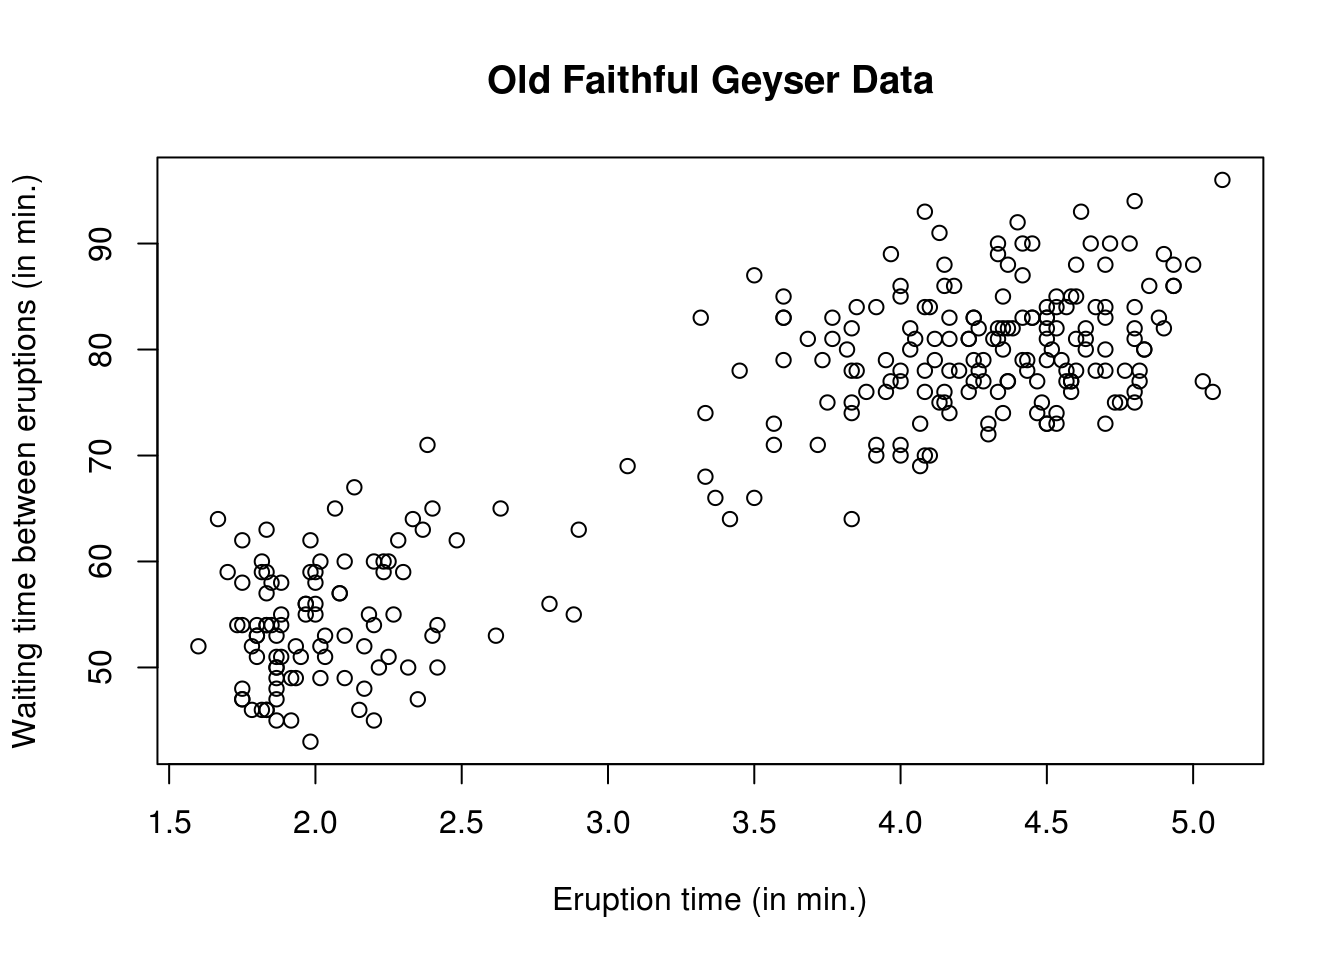
\includegraphics[width=0.7\linewidth]{LineaRModels_files/figure-latex/week1_scatterplot-1} \end{center}

\begin{Shaded}
\begin{Highlighting}[]
\CommentTok{#using the grammar of graphics (more modular)}
\CommentTok{#install.packages("ggplot2") #do this once only}
\KeywordTok{library}\NormalTok{(ggplot2)}
\NormalTok{ggplot2}\OperatorTok{::}\KeywordTok{ggplot}\NormalTok{(}\DataTypeTok{data =}\NormalTok{ faithful, }\KeywordTok{aes}\NormalTok{(}\DataTypeTok{x =}\NormalTok{ eruptions, }\DataTypeTok{y =}\NormalTok{ waiting)) }\OperatorTok{+}\StringTok{ }
\StringTok{  }\KeywordTok{geom_point}\NormalTok{() }\OperatorTok{+}\StringTok{  }
\StringTok{  }\KeywordTok{labs}\NormalTok{(}\DataTypeTok{title =} \StringTok{"Old Faithful Geyser Data"}\NormalTok{, }
       \DataTypeTok{x =} \StringTok{"Eruption time (in min.)"}\NormalTok{, }
       \DataTypeTok{y =} \StringTok{"Waiting time between eruptions (in min.)"}\NormalTok{)}
\end{Highlighting}
\end{Shaded}

\begin{center}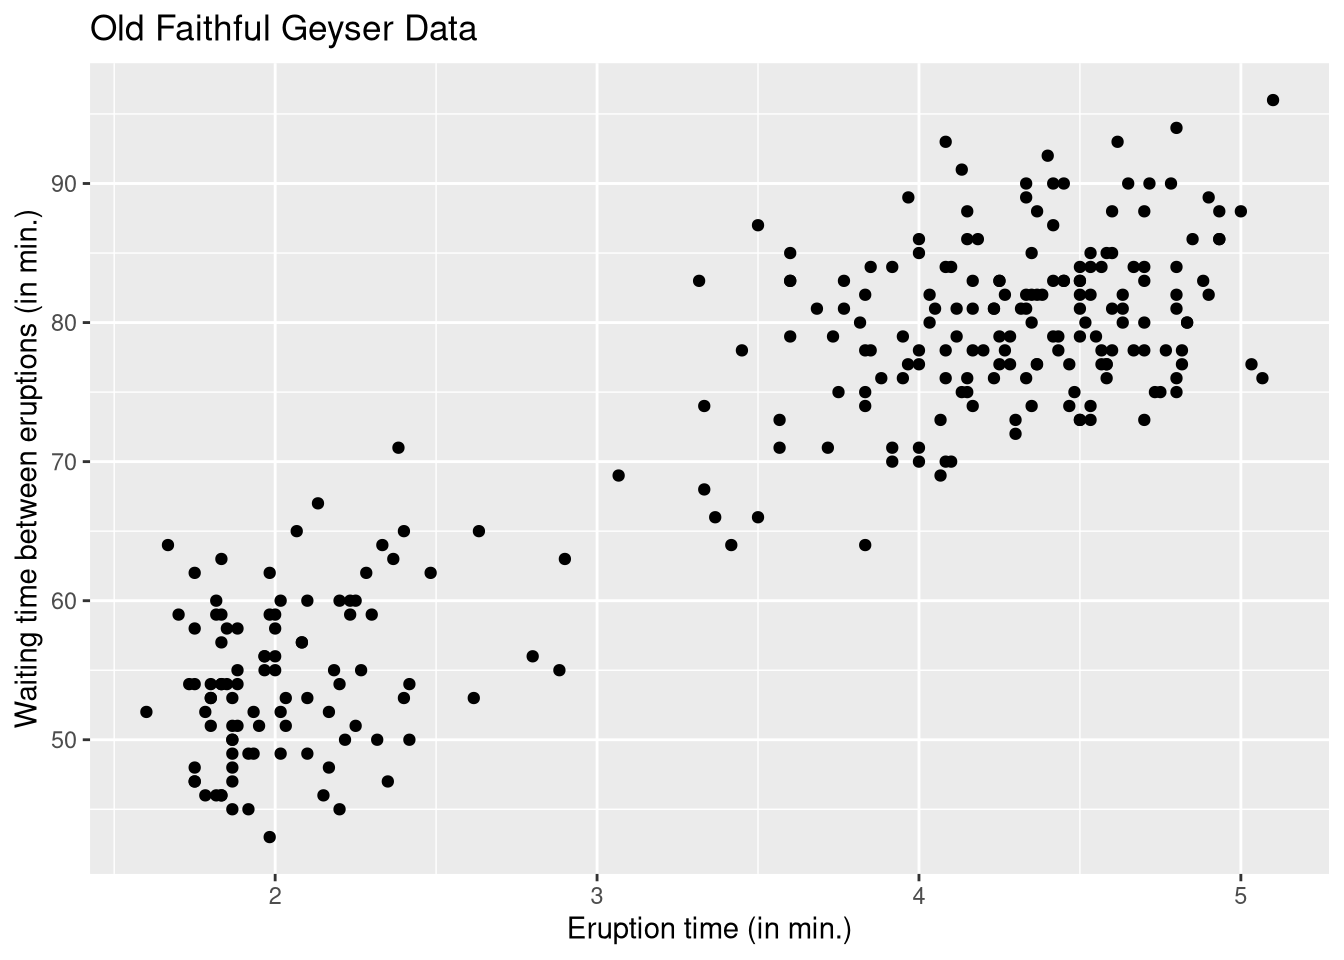
\includegraphics[width=0.7\linewidth]{LineaRModels_files/figure-latex/week1_scatterplot-2} \end{center}

A simple linear model of the form \[y_i = \beta_0 + \beta_1 \mathrm{x}_i + \varepsilon_i,\] where \(\varepsilon_i\) is a noise variable with expectation zero and \(\mathbf{x} = \mathsf{eruptions}\) and \(\boldsymbol{y} = \mathsf{waiting}\). We first create a matrix with a column of \(\mathbf{1}_n\) for the intercept. We bind vectors by column (\texttt{cbind}) into a matrix, recycling arguments if necessary. Use \texttt{\$} to obtain a column of the data frame based on the name of the variable (partial matching is allowed, e.g., \texttt{faithful\$er} is equivalent to \texttt{faithful\$eruptions} in this case).

\begin{Shaded}
\begin{Highlighting}[]
\CommentTok{## Manipulating matrices}
\NormalTok{n <-}\StringTok{ }\KeywordTok{nrow}\NormalTok{(faithful)}
\NormalTok{p <-}\StringTok{ }\KeywordTok{ncol}\NormalTok{(faithful)}
\NormalTok{y <-}\StringTok{ }\NormalTok{faithful}\OperatorTok{$}\NormalTok{waiting}
\NormalTok{X <-}\StringTok{ }\KeywordTok{cbind}\NormalTok{(}\DecValTok{1}\NormalTok{, faithful}\OperatorTok{$}\NormalTok{eruptions)}
\end{Highlighting}
\end{Shaded}

\hypertarget{projection-matrices}{%
\subsection{Projection matrices}\label{projection-matrices}}

Recall that \(\mathbf{H}_{\mathbf{X}} \equiv \mathbf{X}(\mathbf{X}^\top\mathbf{X})^{-1}\mathbf{X}^\top\) is the orthogonal projection matrix onto
\(\mathsf{span}(\mathbf{X})\). The latter has \(p=2\) eigenvalues equal to 1, is an \(n \times n\) matrix of rank \(p\), is symmetric and idempotent.

\BeginKnitrBlock{rmdnote}
\(\mathbf{H}_{\mathbf{X}}\) is a great theoretical tool, but make no mistake: we will never use it in practice other than to verify statements made in class. The underlying reason is that it is an \(n \times n\) matrix, so storage is costly if \(n\) is large. In practice, there are other ways to obtain quantities of interest such as coefficients, residuals and fitted values.
\EndKnitrBlock{rmdnote}

We can verify the properties of \(\mathbf{H}_{\mathbf{X}}\) numerically.

\BeginKnitrBlock{rmdcaution}
Whereas we will frequently use \texttt{==} to check for equality of booleans, the latter should be avoided for comparisons because computer arithmetic is exact only in base 2. For example, \texttt{1/10\ +\ 2/10\ -\ 3/10\ ==\ 0} will return \texttt{FALSE}, whereas \texttt{all.equal(1/10\ +\ 2/10\ -\ 3/10,\ 0)} will return \texttt{TRUE}.
Use \texttt{all.equal} to check for equalities.
\EndKnitrBlock{rmdcaution}

\begin{Shaded}
\begin{Highlighting}[]
\NormalTok{Hx <-}\StringTok{ }\NormalTok{X }\OperatorTok\StringTok{ }\KeywordTok{solve}\NormalTok{(}\KeywordTok{crossprod}\NormalTok{(X)) }\OperatorTok\StringTok{ }\KeywordTok{t}\NormalTok{(X)}
\CommentTok{# Create projection matrix onto complement }
\CommentTok{# `diag(n)` is the n by n identity matrix}
\NormalTok{Mx <-}\StringTok{ }\KeywordTok{diag}\NormalTok{(n) }\OperatorTok{-}\StringTok{ }\NormalTok{Hx}
\CommentTok{#Check that projection leaves X invariant}
\KeywordTok{isTRUE}\NormalTok{(}\KeywordTok{all.equal}\NormalTok{(X, Hx }\OperatorTok\StringTok{ }\NormalTok{X))}
\end{Highlighting}
\end{Shaded}

\begin{verbatim}
## [1] TRUE
\end{verbatim}

\begin{Shaded}
\begin{Highlighting}[]
\CommentTok{#Check that orthogonal projection maps X to zero matrix of dimension (n, p)}
\KeywordTok{isTRUE}\NormalTok{(}\KeywordTok{all.equal}\NormalTok{(}\KeywordTok{matrix}\NormalTok{(}\DecValTok{0}\NormalTok{, }\DataTypeTok{nrow =}\NormalTok{ n, }\DataTypeTok{ncol =}\NormalTok{ p), Mx }\OperatorTok\StringTok{ }\NormalTok{X))}
\end{Highlighting}
\end{Shaded}

\begin{verbatim}
## [1] TRUE
\end{verbatim}

\begin{Shaded}
\begin{Highlighting}[]
\CommentTok{#Check that the matrix Hx is idempotent}
\KeywordTok{isTRUE}\NormalTok{(}\KeywordTok{all.equal}\NormalTok{(Hx }\OperatorTok\StringTok{ }\NormalTok{Hx, Hx))}
\end{Highlighting}
\end{Shaded}

\begin{verbatim}
## [1] TRUE
\end{verbatim}

\begin{Shaded}
\begin{Highlighting}[]
\CommentTok{#Check that the matrix Hx is symmetric}
\KeywordTok{isTRUE}\NormalTok{(}\KeywordTok{all.equal}\NormalTok{(}\KeywordTok{t}\NormalTok{(Hx), Hx))}
\end{Highlighting}
\end{Shaded}

\begin{verbatim}
## [1] TRUE
\end{verbatim}

\begin{Shaded}
\begin{Highlighting}[]
\CommentTok{#Check that only a two eigenvalue are 1 and the rest are zero}
\KeywordTok{isTRUE}\NormalTok{(}\KeywordTok{all.equal}\NormalTok{(}\KeywordTok{eigen}\NormalTok{(Hx, }\DataTypeTok{only.values =} \OtherTok{TRUE}\NormalTok{)}\OperatorTok{$}\NormalTok{values, }\KeywordTok{c}\NormalTok{(}\KeywordTok{rep}\NormalTok{(}\DecValTok{1}\NormalTok{, p), }\KeywordTok{rep}\NormalTok{(}\DecValTok{0}\NormalTok{, n }\OperatorTok{-}\StringTok{ }\NormalTok{p))))}
\end{Highlighting}
\end{Shaded}

\begin{verbatim}
## [1] TRUE
\end{verbatim}

\begin{Shaded}
\begin{Highlighting}[]
\CommentTok{#Check that the matrix has rank p}
\KeywordTok{isTRUE}\NormalTok{(}\KeywordTok{all.equal}\NormalTok{(Matrix}\OperatorTok{::}\KeywordTok{rankMatrix}\NormalTok{(Hx), p, }\DataTypeTok{check.attributes =} \OtherTok{FALSE}\NormalTok{))}
\end{Highlighting}
\end{Shaded}

\begin{verbatim}
## [1] TRUE
\end{verbatim}

\BeginKnitrBlock{rmdcaution}
Be careful: if \texttt{A} is an \(n \times p\) matrix, \texttt{length(A)} returns the number of elements in the matrix, meaning \(np\). Use \texttt{nrow(A)} for the number of observations.
\EndKnitrBlock{rmdcaution}

\hypertarget{exercises}{%
\section{Exercises}\label{exercises}}

\hypertarget{auto-dataset}{%
\subsection{Auto dataset}\label{auto-dataset}}

\begin{itemize}
\tightlist
\item
  Install the \textbf{R} package \texttt{ISLR} and load the dataset \texttt{Auto}. Be careful, as \textbf{R} is case-sensitive.
\item
  Query the help file for information about the dataset.
\item
  Look at the first lines of \texttt{Auto}
\item
  Create an explanatory variable \texttt{x} with horsepower and mileage per gallon as response \texttt{y}.
\item
  Create a scatterplot of \texttt{y} against \texttt{x}. Is there evidence of a linear relationship between the two variables?
\item
  Append a column vector of ones to \texttt{x} and create a projection matrix.
\item
  Check that the resulting projection matrix is symmetric and idempotent.
\end{itemize}

\hypertarget{solutions}{%
\section{Solutions}\label{solutions}}

\hypertarget{exercise-1.4---oblique-projections}{%
\subsection{Exercise 1.4 - Oblique projections}\label{exercise-1.4---oblique-projections}}

Suppose that \(\mathsf{span}(\mathbf{X}) \neq \mathsf{span}(\mathbf{W})\), that both \(\mathbf{X}\) and \(\mathbf{W}\) are full-rank \(n \times p\) matrices such that \(\mathbf{X}^\top\mathbf{W}\) and \(\mathbf{W}^\top\mathbf{X}\) are invertible. An oblique projection matrix is of the form \(\mathbf{P}\equiv\mathbf{X}(\mathbf{W}^\top\mathbf{X})^{-1}\mathbf{W}^\top\) and appears in instrumental variable regression. The oblique projection is such that \(\mathrm{im}(\mathbf{P})=\mathsf{span}(\mathbf{X})\), but \(\mathrm{im}(\mathbf{I}-\mathbf{P})=\mathsf{span}(\mathbf{W}^\perp)\). This fact is illustrated below.

We consider two non-parallel vectors in \(\mathbb{R}^2\), \(\mathbf{X}\) and \(\mathbf{W}\).

\begin{Shaded}
\begin{Highlighting}[]
\CommentTok{#Create two vectors (non-parallel)}
\NormalTok{x <-}\StringTok{ }\KeywordTok{c}\NormalTok{(}\DecValTok{1}\NormalTok{, }\DecValTok{2}\NormalTok{)}
\NormalTok{w <-}\StringTok{ }\KeywordTok{c}\NormalTok{(}\OperatorTok{-}\DecValTok{1}\NormalTok{, }\FloatTok{0.1}\NormalTok{)}
\CommentTok{#Create oblique projection matrix}
\NormalTok{P <-}\StringTok{ }\NormalTok{x }\OperatorTok\StringTok{ }\KeywordTok{solve}\NormalTok{(}\KeywordTok{t}\NormalTok{(w) }\OperatorTok\StringTok{ }\NormalTok{x) }\OperatorTok\StringTok{ }\KeywordTok{t}\NormalTok{(w)}

\KeywordTok{isTRUE}\NormalTok{(}\KeywordTok{all.equal}\NormalTok{((P }\OperatorTok\StringTok{ }\NormalTok{P), P)) }\CommentTok{#P is idempotent}
\end{Highlighting}
\end{Shaded}

\begin{verbatim}
## [1] TRUE
\end{verbatim}

\begin{Shaded}
\begin{Highlighting}[]
\NormalTok{P }\OperatorTok{-}\StringTok{ }\KeywordTok{t}\NormalTok{(P) }\CommentTok{#but not symmetric}
\end{Highlighting}
\end{Shaded}

\begin{verbatim}
##       [,1]   [,2]
## [1,] 0.000 -2.625
## [2,] 2.625  0.000
\end{verbatim}

The figure below shows the projection of a third vector \(\mathbf{v}\) (non-parallel to \(\mathbf{X}\) or \(\mathbf{W}\)) onto the span of {\(\mathbf{P}\) (blue)}, {\(\mathbf{P}^\top\) (red)}, {\(\mathbf{I}_2-\mathbf{P}\) (dashed cyan)} and {\(\mathbf{I}_2-\mathbf{P}^\top\) (dashed orange)}. The circles indicate the vectors {\(\mathbf{W}\) (red)} and {\(\mathbf{X}\) (blue)} on the plane. Notice that \(\mathbf{I}_2-\mathbf{P}^\top \perp \mathbf{P}\), whereas \(\mathbf{I}_2-\mathbf{P} \perp \mathbf{P}^\top\).

\begin{center}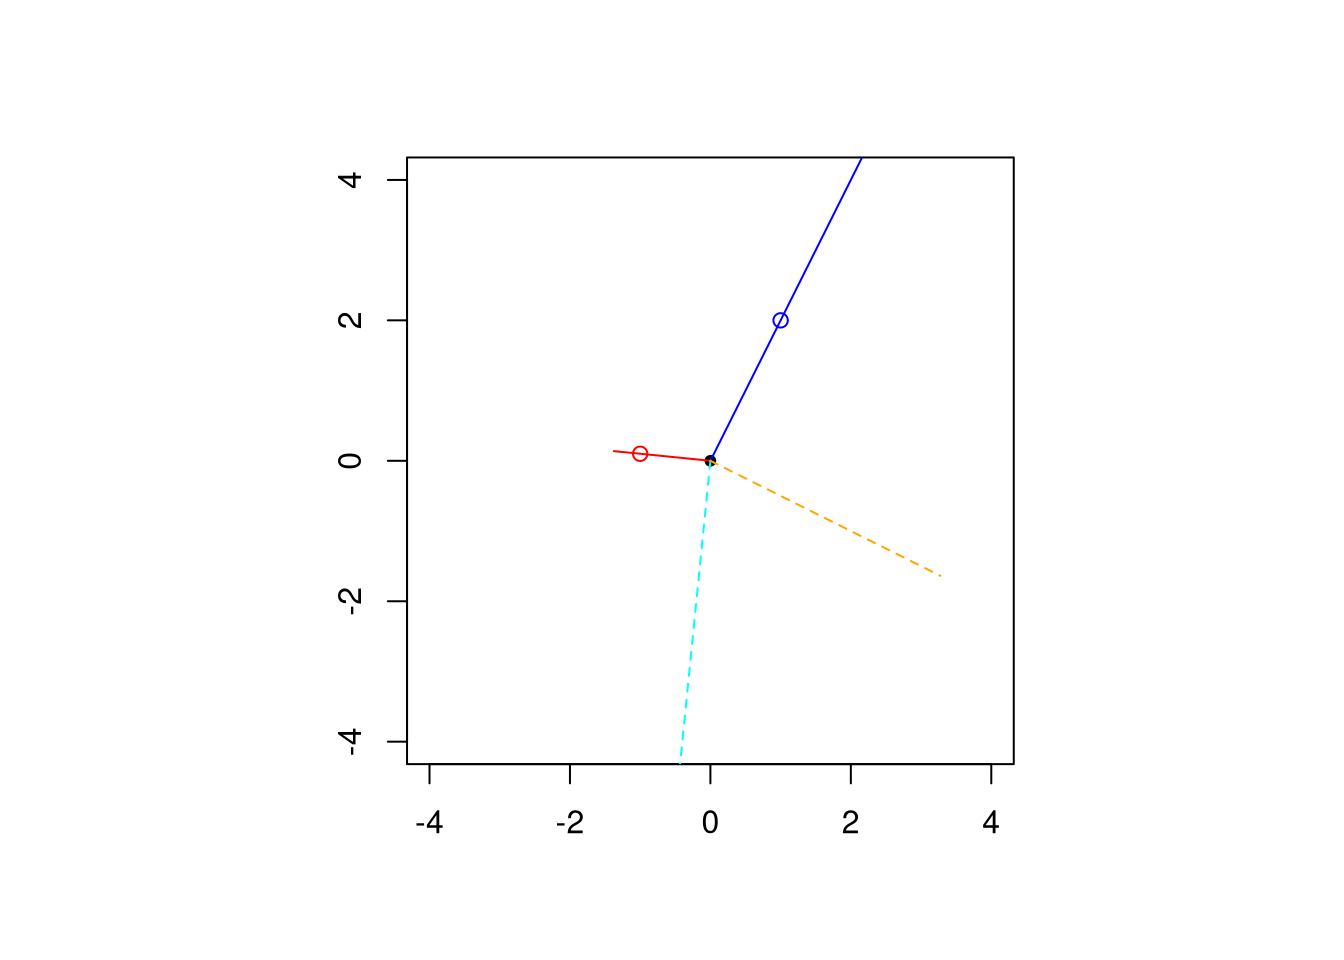
\includegraphics[width=0.7\linewidth]{LineaRModels_files/figure-latex/illustproj-1} \end{center}

\hypertarget{summary-of-week-1}{%
\section{Summary of week 1}\label{summary-of-week-1}}

Let \(\mathbf{X}\) be an \(n \times p\) full-rank matrix (\(p <n\)). An \(n \times n\) orthogonal projection matrix \(\mathbf{H}\)

\begin{itemize}
\tightlist
\item
  projects on to \(\mathcal{V} \subseteq \mathbb{R}^n\), meaning \(\mathbf{Hv} \in \mathcal{V}\) for any \(\mathbf{v} \in \mathbb{R}^n\);
\item
  is idempotent, meaning \(\mathbf{H} = \mathbf{HH}\);
\item
  is symmetric, meaning \(\mathbf{H} = \mathbf{H}^\top\).
\end{itemize}

The projection matrix \(\mathbf{H}\) is unique; if \(\mathcal{V} = \mathscr{S}(\mathbf{X})\), then
\[\mathbf{H}_{\mathbf{X}} = \mathbf{X}(\mathbf{X}^\top\mathbf{X})^{-1}\mathbf{X}^\top.\]
Since \(\mathbf{X}: \mathbb{R}^n \to \mathbb{R}^p\), \(\mathbf{H}_{\mathbf{X}}\) has rank \(p\). The orthogonal complement \(\mathbf{M}_{\mathbf{X}}\equiv \mathbf{I}_n - \mathbf{H}_{\mathbf{X}}\) projects onto \(\mathscr{S}^{\perp}(\mathbf{X})\).

\hypertarget{computational-considerations}{%
\chapter{Computational considerations}\label{computational-considerations}}

In this tutorial, we will explore some basic \textbf{R} commands and illustrate their use on the Auto dataset (\texttt{Auto}) from the \texttt{ISLR} package.

\hypertarget{calculation-of-least-square-estimates}{%
\section{Calculation of least square estimates}\label{calculation-of-least-square-estimates}}

Consider as usual \(\boldsymbol{y}\) and \(n\)-vector of response variables and a full-rank \(n \times p\) design matrix \(\mathbf{X}\). We are interested in finding the ordinary least square coefficient \(\hat{\boldsymbol{\beta}}\), the fitted values \(\hat{\boldsymbol{y}} = \mathbf{X}\hat{\boldsymbol{\beta}}\) and the residuals \(\boldsymbol{e} = \boldsymbol{y} - \mathbf{X}\boldsymbol{\beta}\).

Whereas orthogonal projection matrices are useful for theoretical derivations, they are not used for computations. Building \(\mathbf{H}_{\mathbf{X}}\) involves a matrix inversion and the storage of an \(n \times n\) matrix. In Exercise series 2, we looked at two matrix decompositions: a singular value decomposition (SVD) and a QR decomposition. These are more numerically stable than using the normal equations \((\mathbf{X}^\top\mathbf{X})\boldsymbol{\beta} = \mathbf{X}^\top\boldsymbol{y}\) (the condition number of the matrix \(\mathbf{X}^\top\mathbf{X}\) is the square of that of \(\mathbf{X}\) --- more on this later).
The code related to the SVD and QR decompositions is provided for reference, so you can validate the derivations in the exercise. You won't need it in practice.

\textbf{Optional} material: for more details about the complexity and algorithms underlying the different methods, the reader is referred to these notes of \href{www.math.uchicago.edu/~may/REU2012/REUPapers/Lee.pdf}{Lee}.

We can fit a simple linear model with an intercept and a linear effect for the weight,
\[ \texttt{mpg}_i = \beta_0 + \texttt{hp}_i\beta_1 +\varepsilon_i.\]

We form the design matrix \((\boldsymbol{1}_n^\top, \texttt{hp}^\top)^\top\) and the vector of regressand \(\texttt{mpg}\), then proceed with calculating the OLS coefficients \(\hat{\boldsymbol{\beta}}\), the fitted values \(\hat{\boldsymbol{y}}\) and the residuals \(\boldsymbol{e}\).

We can compute first the ordinary least square estimates using the formula \(\hat{\boldsymbol{\beta}} = (\mathbf{X}^\top\mathbf{X})^{-1}\mathbf{X}^\top\boldsymbol{y}\). The fitted values are \(\hat{\boldsymbol{y}} = \mathbf{X}\hat{\boldsymbol{\beta}}\) and the residuals \(\boldsymbol{e} = \boldsymbol{y} - \hat{\boldsymbol{y}}\).

\begin{Shaded}
\begin{Highlighting}[]
\KeywordTok{data}\NormalTok{(Auto, }\DataTypeTok{package =} \StringTok{"ISLR"}\NormalTok{)}
\NormalTok{y <-}\StringTok{ }\NormalTok{Auto}\OperatorTok{$}\NormalTok{mpg}
\NormalTok{X <-}\StringTok{ }\KeywordTok{cbind}\NormalTok{(}\DecValTok{1}\NormalTok{, Auto}\OperatorTok{$}\NormalTok{horsepower)}
\NormalTok{n <-}\StringTok{ }\KeywordTok{nrow}\NormalTok{(X)}
\NormalTok{p <-}\StringTok{ }\KeywordTok{ncol}\NormalTok{(X)}
\CommentTok{# Estimation of beta_hat:}
\NormalTok{XtX <-}\StringTok{ }\KeywordTok{crossprod}\NormalTok{(X)}
\NormalTok{Xty <-}\StringTok{ }\KeywordTok{crossprod}\NormalTok{(X, y)}
\CommentTok{# Solve normal equations}
\NormalTok{beta_hat <-}\StringTok{ }\KeywordTok{as.vector}\NormalTok{(}\KeywordTok{solve}\NormalTok{(XtX, Xty))}
\CommentTok{#same as beta_hat <- solve(t(X) %*% X) %*% t(X) %*% y}

\CommentTok{##Create residuals and fitted values}
\NormalTok{fitted <-}\StringTok{ }\KeywordTok{as.vector}\NormalTok{(X }\OperatorTok\StringTok{ }\NormalTok{beta_hat)}
\NormalTok{res <-}\StringTok{ }\NormalTok{y }\OperatorTok{-}\StringTok{ }\NormalTok{fitted}
\end{Highlighting}
\end{Shaded}

The residuals \(\boldsymbol{e} = \boldsymbol{y} -\hat{\boldsymbol{y}}\) can be interpreted as the \emph{vertical} distance between the regression slope and the observation. For each observation \(y_i\), a vertical line at distance \(e_i\) is drawn from the prediction \(\hat{y}_i\).

\begin{Shaded}
\begin{Highlighting}[]
\KeywordTok{plot}\NormalTok{(mpg }\OperatorTok{~}\StringTok{ }\NormalTok{horsepower,  }\DataTypeTok{data =}\NormalTok{ Auto, }
     \DataTypeTok{xlab =} \StringTok{"Power of engine (hp)"}\NormalTok{, }
     \DataTypeTok{ylab =} \StringTok{"Fuel economy (miles/US gallon)"}\NormalTok{, }
     \DataTypeTok{main =} \StringTok{"Fuel economy of automobiles"}\NormalTok{,}
     \DataTypeTok{ylim =} \KeywordTok{c}\NormalTok{(}\DecValTok{0}\NormalTok{, }\DecValTok{50}\NormalTok{),}
     \CommentTok{# the subsequent commands for `plot`  tweak the display}
     \CommentTok{# check for yourself the effect of removing them}
     \CommentTok{# bty = "l" gives L shaped graphical windows (not boxed)}
     \CommentTok{# pch = 20 gives full dots rather than empty circles for points}
     \DataTypeTok{bty =} \StringTok{"l"}\NormalTok{, }\DataTypeTok{pch =} \DecValTok{20}\NormalTok{) }
\CommentTok{#Line of best linear fit}
\KeywordTok{abline}\NormalTok{(}\DataTypeTok{a =}\NormalTok{ beta_hat[}\DecValTok{1}\NormalTok{], }\DataTypeTok{b =}\NormalTok{ beta_hat[}\DecValTok{2}\NormalTok{])}

\CommentTok{#Residuals are vertical distance from line to }
\ControlFlowTok{for}\NormalTok{(i }\ControlFlowTok{in} \DecValTok{1}\OperatorTok{:}\KeywordTok{nrow}\NormalTok{(X))\{}
  \KeywordTok{segments}\NormalTok{(}\DataTypeTok{x0 =}\NormalTok{ Auto}\OperatorTok{$}\NormalTok{horsepower[i], }\DataTypeTok{y0 =}\NormalTok{ fitted[i], }\DataTypeTok{y1 =}\NormalTok{ fitted[i] }\OperatorTok{+}\StringTok{ }\NormalTok{res[i], }\DataTypeTok{col =} \DecValTok{2}\NormalTok{)}
\NormalTok{\}}
\end{Highlighting}
\end{Shaded}

\begin{center}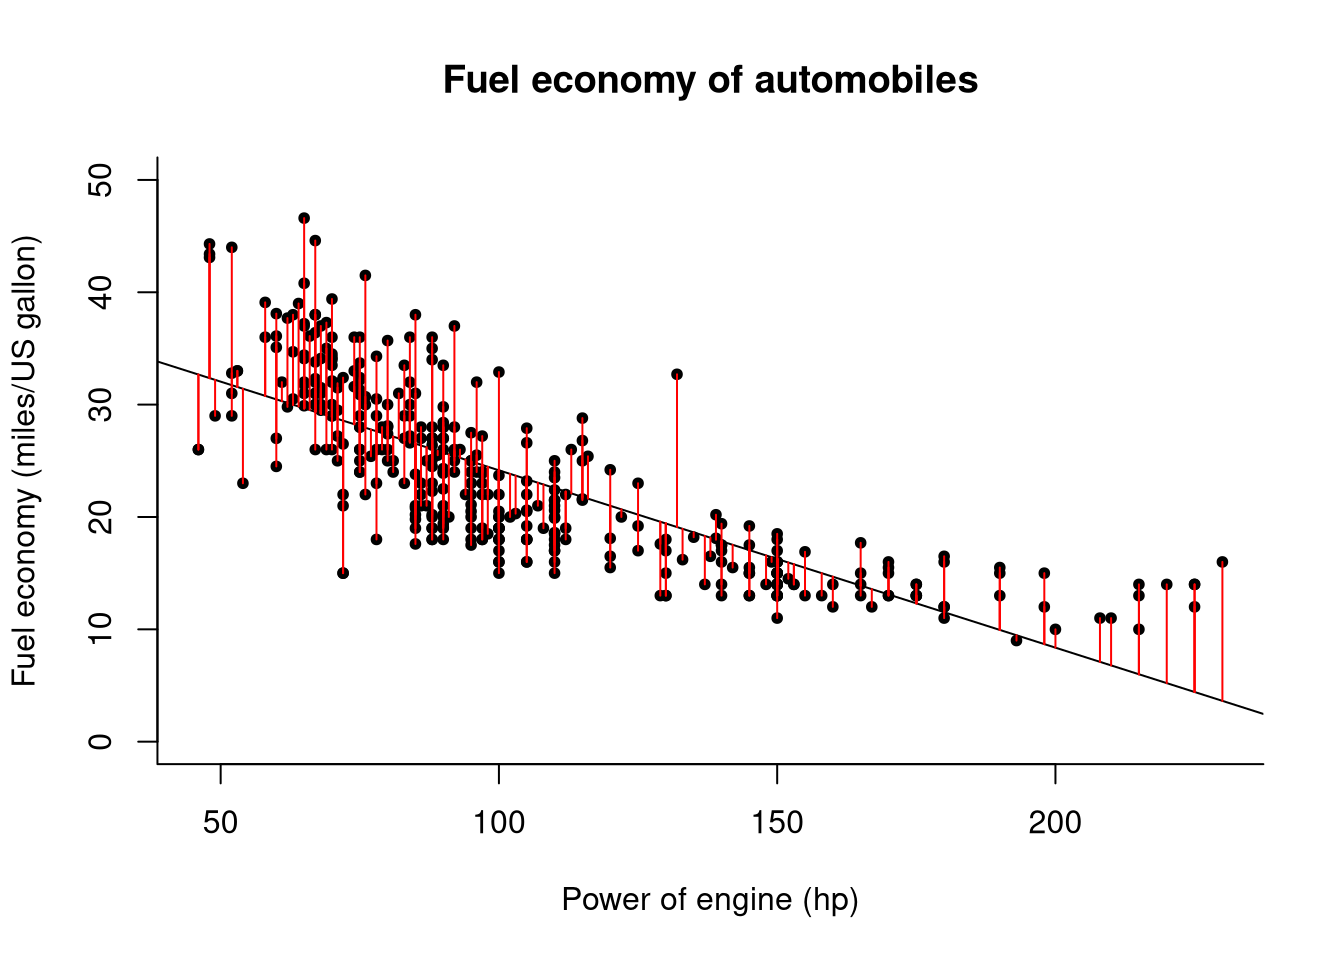
\includegraphics[width=0.7\linewidth]{LineaRModels_files/figure-latex/verticaldist-1} \end{center}

The same scatterplot, this time using \texttt{ggplot2}.

\begin{Shaded}
\begin{Highlighting}[]
\KeywordTok{library}\NormalTok{(ggplot2, }\DataTypeTok{warn.conflicts =} \OtherTok{FALSE}\NormalTok{, }\DataTypeTok{quietly =} \OtherTok{TRUE}\NormalTok{)}
\CommentTok{#Create data frame with segments}
\NormalTok{vlines <-}\StringTok{ }\KeywordTok{data.frame}\NormalTok{(}\DataTypeTok{x1 =}\NormalTok{ Auto}\OperatorTok{$}\NormalTok{horsepower, }\DataTypeTok{y1 =}\NormalTok{ fitted, }\DataTypeTok{y2 =}\NormalTok{ fitted }\OperatorTok{+}\StringTok{ }\NormalTok{res)}
\NormalTok{ggg <-}\StringTok{ }\KeywordTok{ggplot}\NormalTok{(Auto, }\KeywordTok{aes}\NormalTok{(}\DataTypeTok{x =}\NormalTok{ horsepower, }\DataTypeTok{y =}\NormalTok{ mpg)) }\OperatorTok{+}\StringTok{ }
\StringTok{        }\KeywordTok{geom_point}\NormalTok{() }\OperatorTok{+}\StringTok{ }
\StringTok{        }\KeywordTok{labs}\NormalTok{(}\DataTypeTok{x =} \StringTok{"Power of engine (hp)"}\NormalTok{, }
             \DataTypeTok{y =} \StringTok{"Fuel economy (miles/US gallon)"}\NormalTok{, }
             \DataTypeTok{title =} \StringTok{"Fuel economy of automobiles"}\NormalTok{) }\OperatorTok{+}
\StringTok{      }\KeywordTok{geom_segment}\NormalTok{(}\KeywordTok{aes}\NormalTok{(}\DataTypeTok{x =}\NormalTok{ x1, }\DataTypeTok{y =}\NormalTok{ y1, }\DataTypeTok{xend =}\NormalTok{ x1, }\DataTypeTok{yend =}\NormalTok{ y2, }\DataTypeTok{color =} \StringTok{"red"}\NormalTok{), }
                   \DataTypeTok{data =}\NormalTok{ vlines, }\DataTypeTok{show.legend =} \OtherTok{FALSE}\NormalTok{) }\OperatorTok{+}\StringTok{ }
\StringTok{      }\KeywordTok{geom_abline}\NormalTok{(}\DataTypeTok{slope =}\NormalTok{ beta_hat[}\DecValTok{2}\NormalTok{], }\DataTypeTok{intercept =}\NormalTok{ beta_hat[}\DecValTok{1}\NormalTok{])}
\KeywordTok{print}\NormalTok{(ggg)}
\end{Highlighting}
\end{Shaded}

\begin{center}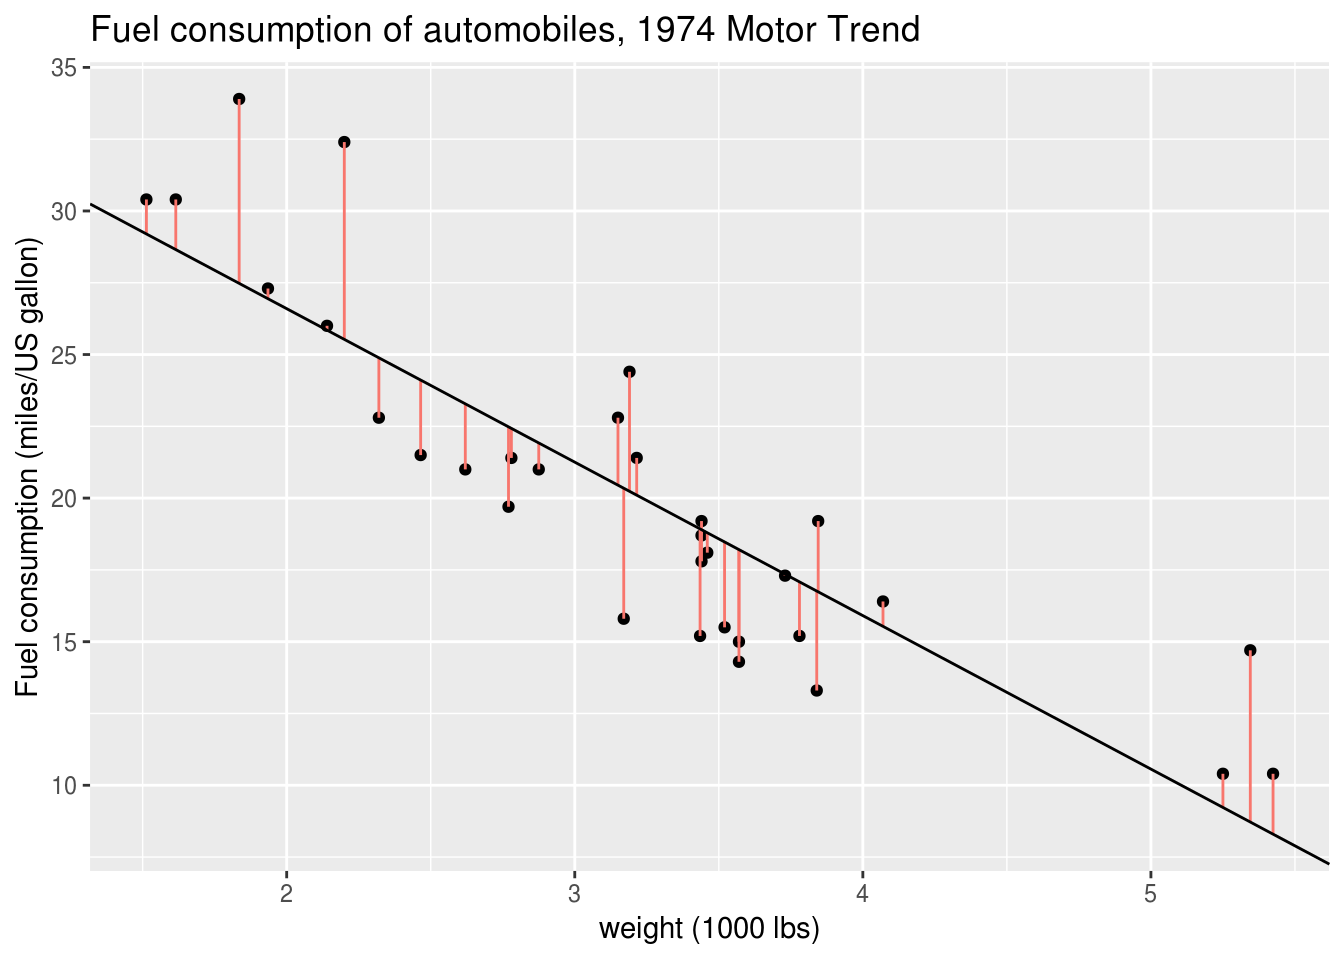
\includegraphics[width=0.7\linewidth]{LineaRModels_files/figure-latex/ggplotmtcars-1} \end{center}

\hypertarget{interpretation-of-the-coefficients}{%
\subsection{Interpretation of the coefficients}\label{interpretation-of-the-coefficients}}

If the regression model is
\[y_i = \beta_0 + \mathrm{x}_{i1}\beta_1 + \mathrm{x}_{i2}\beta_2 + \varepsilon_i,\] the interpretation of \(\beta_1\) in the linear model is as follows: a unit increase in \(x\) leads to \(\beta_1\) units increase in \(y\), everything else (i.e., \(\mathrm{x}_{i2}\)) being held constant.

For the \texttt{Auto} regression above, an increase of the power of the engine by one horsepower leads to an average decrease of 0.16 miles per US gallon in distance covered by the car. We could easily get an equivalent statement in terms of increase of the car fuel consumption for a given distance.

\hypertarget{the-lm-function}{%
\section{\texorpdfstring{The \texttt{lm} function}{The lm function}}\label{the-lm-function}}

The function \texttt{lm} is the workshorse for fitting linear models. It takes as input a formula: suppose you have a data frame containing columns \texttt{x} (a regressor) and \texttt{y} (the regressand); you can then call \texttt{lm(y\ \textasciitilde{}\ x)} to fit the linear model \(y = \beta_0 + \beta_1x + \varepsilon\). The explanatory variable \texttt{y} is on the left hand side,
while the right hand side should contain the predictors, separated by a \texttt{+} sign if there are more than one.
If you provide the data frame name using \texttt{data}, then the shorthand \texttt{y\ \textasciitilde{}\ .} fits all the columns of the data frame (but \texttt{y}) as regressors.

To fit higher order polynomials or transformations, use the \texttt{I} function to tell \textbf{R} to interpret the input ``as is''.
Thus, \texttt{lm(y\textasciitilde{}x+I(x\^{}2))}, would fit a linear model with design matrix \((\boldsymbol{1}_n, \mathbf{x}^\top, \mathbf{x}^2)^\top\). A constant is automatically included in the regression, but can be removed by writing \texttt{-1} or \texttt{+0} on the right hand side of the formula.

\begin{Shaded}
\begin{Highlighting}[]
\CommentTok{# The function lm and its output}
\NormalTok{fit <-}\StringTok{ }\KeywordTok{lm}\NormalTok{(mpg }\OperatorTok{~}\StringTok{ }\NormalTok{horsepower }\OperatorTok{+}\StringTok{ }\KeywordTok{I}\NormalTok{(horsepower}\OperatorTok{^}\DecValTok{2}\NormalTok{), }\DataTypeTok{data =}\NormalTok{ Auto)}
\NormalTok{fit_summary <-}\StringTok{ }\KeywordTok{summary}\NormalTok{(fit)}
\end{Highlighting}
\end{Shaded}

The \texttt{lm} output will display OLS estimates along with standard errors, \(t\) values for the Wald test of the hypothesis \(\mathrm{H}_0: \beta_i=0\) and the associated \(P\)-values. Other statistics and information about the sample size, the degrees of freedom, etc., are given at the bottom of the table.

Many methods allow you to extract specific objects. For example, the functions \texttt{coef}, \texttt{resid}, \texttt{fitted}, \texttt{model.matrix} will return \(\hat{\boldsymbol{\beta}}\), \(\boldsymbol{e}\), \(\hat{\boldsymbol{y}}\) and \(\mathbf{X}\), respectively.

\begin{Shaded}
\begin{Highlighting}[]
\KeywordTok{names}\NormalTok{(fit)}
\end{Highlighting}
\end{Shaded}

\begin{verbatim}
##  [1] "coefficients"  "residuals"     "effects"       "rank"         
##  [5] "fitted.values" "assign"        "qr"            "df.residual"  
##  [9] "xlevels"       "call"          "terms"         "model"
\end{verbatim}

\begin{Shaded}
\begin{Highlighting}[]
\KeywordTok{names}\NormalTok{(fit_summary)}
\end{Highlighting}
\end{Shaded}

\begin{verbatim}
##  [1] "call"          "terms"         "residuals"     "coefficients" 
##  [5] "aliased"       "sigma"         "df"            "r.squared"    
##  [9] "adj.r.squared" "fstatistic"    "cov.unscaled"
\end{verbatim}

The following simply illustrates what has been derived in Exercise series 2. \textbf{R} has devoted functions that are coded more efficiently.

\hypertarget{singular-value-decomposition}{%
\subsection{Singular value decomposition}\label{singular-value-decomposition}}

The SVD decomposition in \textbf{R} returns a list with elements \texttt{u}, \texttt{d} and \texttt{v}. \texttt{u} is the orthonormal \(n \times p\) matrix, \texttt{d} is a vector containing the diagonal elements of \(\mathbf{D}\) and \texttt{v} is the \(p \times p\) orthogonal matrix. Recall that the decomposition is
\[\mathbf{X} = \mathbf{UDV}^\top\]
and that \(\mathbf{VV}^\top= \mathbf{V}^\top\mathbf{V}=\mathbf{U}^\top\mathbf{U}=\mathbf{I}_p\). The matrix \(\mathbf{D}\) contains the singular values of \(\mathbf{X}\), and the diagonal elements \(\mathrm{d}_{ii}^2\) corresponds to the (ordered) eigenvalues of \(\mathbf{X}^\top\mathbf{X}\).

The following shows how to use the SVD decomposition in \textbf{R}. This material is \textbf{optional} and provided for reference only.

\begin{Shaded}
\begin{Highlighting}[]
\NormalTok{svdX <-}\StringTok{ }\KeywordTok{svd}\NormalTok{(X)}
\CommentTok{# Projection matrix}
\NormalTok{Hx <-}\StringTok{ }\KeywordTok{tcrossprod}\NormalTok{(svdX}\OperatorTok{$}\NormalTok{u)}
\CommentTok{# t(U) %*% U gives p by p identity matrix}
\KeywordTok{all.equal}\NormalTok{(}\KeywordTok{crossprod}\NormalTok{(svdX}\OperatorTok{$}\NormalTok{u), }\KeywordTok{diag}\NormalTok{(p))}
\end{Highlighting}
\end{Shaded}

\begin{verbatim}
## [1] TRUE
\end{verbatim}

\begin{Shaded}
\begin{Highlighting}[]
\CommentTok{# V is an orthogonal matrix}
\KeywordTok{all.equal}\NormalTok{(}\KeywordTok{tcrossprod}\NormalTok{(svdX}\OperatorTok{$}\NormalTok{v), }\KeywordTok{diag}\NormalTok{(p))}
\end{Highlighting}
\end{Shaded}

\begin{verbatim}
## [1] TRUE
\end{verbatim}

\begin{Shaded}
\begin{Highlighting}[]
\KeywordTok{all.equal}\NormalTok{(}\KeywordTok{crossprod}\NormalTok{(svdX}\OperatorTok{$}\NormalTok{v), }\KeywordTok{diag}\NormalTok{(p))}
\end{Highlighting}
\end{Shaded}

\begin{verbatim}
## [1] TRUE
\end{verbatim}

\begin{Shaded}
\begin{Highlighting}[]
\CommentTok{# D contains singular values}
\KeywordTok{all.equal}\NormalTok{(svdX}\OperatorTok{$}\NormalTok{d}\OperatorTok{^}\DecValTok{2}\NormalTok{, }\KeywordTok{eigen}\NormalTok{(XtX, }\DataTypeTok{only.values =} \OtherTok{TRUE}\NormalTok{)}\OperatorTok{$}\NormalTok{values)}
\end{Highlighting}
\end{Shaded}

\begin{verbatim}
## [1] TRUE
\end{verbatim}

\begin{Shaded}
\begin{Highlighting}[]
\CommentTok{# OLS coefficient from SVD}
\NormalTok{beta_hat_svd <-}\StringTok{ }\KeywordTok{c}\NormalTok{(svdX}\OperatorTok{$}\NormalTok{v }\OperatorTok\StringTok{  }\KeywordTok{diag}\NormalTok{(}\DecValTok{1}\OperatorTok{/}\NormalTok{svdX}\OperatorTok{$}\NormalTok{d) }\OperatorTok\StringTok{ }\KeywordTok{t}\NormalTok{(svdX}\OperatorTok{$}\NormalTok{u) }\OperatorTok\StringTok{ }\NormalTok{y)}
\KeywordTok{all.equal}\NormalTok{(beta_hat_svd, beta_hat)}
\end{Highlighting}
\end{Shaded}

\begin{verbatim}
## [1] TRUE
\end{verbatim}

\hypertarget{qr-decomposition}{%
\subsection{QR decomposition}\label{qr-decomposition}}

\textbf{R} uses a QR-decomposition to calculate the OLS estimates in the function \texttt{lm}. There are specific functions to return coefficients, fitted values and residuals. One can also obtain the \(n \times p\) matrix \(\mathbf{Q}_1\) and the upper triangular \(p \times p\) matrix \(\mathbf{R}\) from the thinned QR decomposition,
\[\mathbf{X} = \mathbf{Q}_1\mathbf{R}.\]

The following shows how to use the QR decomposition in \textbf{R}. This material is \textbf{optional} and provided for reference only.

\begin{Shaded}
\begin{Highlighting}[]
\NormalTok{Hx <-}\StringTok{ }\NormalTok{X }\OperatorTok\StringTok{ }\KeywordTok{solve}\NormalTok{(}\KeywordTok{crossprod}\NormalTok{(X)) }\OperatorTok\StringTok{ }\KeywordTok{t}\NormalTok{(X)}
\NormalTok{qrX <-}\StringTok{ }\KeywordTok{qr}\NormalTok{(X)}
\NormalTok{Q1 <-}\StringTok{ }\KeywordTok{qr.Q}\NormalTok{(qrX)}
\NormalTok{R <-}\StringTok{ }\KeywordTok{qr.R}\NormalTok{(qrX)}
\CommentTok{# Compute beta_hat from QR}
\NormalTok{beta_hat_qr1 <-}\StringTok{ }\KeywordTok{qr.coef}\NormalTok{(qrX, y) }\CommentTok{#using built-in function}
\NormalTok{beta_hat_qr2 <-}\StringTok{ }\KeywordTok{c}\NormalTok{(}\KeywordTok{backsolve}\NormalTok{(R, }\KeywordTok{t}\NormalTok{(Q1) }\OperatorTok\StringTok{ }\NormalTok{y)) }\CommentTok{#manually}
\KeywordTok{all.equal}\NormalTok{(beta_hat, beta_hat_qr1, }\DataTypeTok{check.attributes =} \OtherTok{FALSE}\NormalTok{)}
\end{Highlighting}
\end{Shaded}

\begin{verbatim}
## [1] TRUE
\end{verbatim}

\begin{Shaded}
\begin{Highlighting}[]
\KeywordTok{all.equal}\NormalTok{(beta_hat, beta_hat_qr2, }\DataTypeTok{check.attributes =} \OtherTok{FALSE}\NormalTok{)}
\end{Highlighting}
\end{Shaded}

\begin{verbatim}
## [1] TRUE
\end{verbatim}

\begin{Shaded}
\begin{Highlighting}[]
\CommentTok{# Compute residuals}
\NormalTok{qre <-}\StringTok{ }\KeywordTok{qr.resid}\NormalTok{(qrX, y)}
\KeywordTok{all.equal}\NormalTok{(qre, }\KeywordTok{c}\NormalTok{(y }\OperatorTok{-}\StringTok{ }\NormalTok{X }\OperatorTok\StringTok{ }\NormalTok{beta_hat), }\DataTypeTok{check.attributes =} \OtherTok{FALSE}\NormalTok{)}
\end{Highlighting}
\end{Shaded}

\begin{verbatim}
## [1] TRUE
\end{verbatim}

\begin{Shaded}
\begin{Highlighting}[]
\CommentTok{# Compute fitted values}
\NormalTok{qryhat <-}\StringTok{ }\KeywordTok{qr.fitted}\NormalTok{(qrX, y)}
\KeywordTok{all.equal}\NormalTok{(qryhat, }\KeywordTok{c}\NormalTok{(X }\OperatorTok\StringTok{ }\NormalTok{beta_hat), }\DataTypeTok{check.attributes =} \OtherTok{FALSE}\NormalTok{)}
\end{Highlighting}
\end{Shaded}

\begin{verbatim}
## [1] TRUE
\end{verbatim}

\begin{Shaded}
\begin{Highlighting}[]
\CommentTok{# Compute orthogonal projection matrix}
\NormalTok{qrHx <-}\StringTok{ }\KeywordTok{tcrossprod}\NormalTok{(Q1)}
\KeywordTok{all.equal}\NormalTok{(qrHx, Hx)}
\end{Highlighting}
\end{Shaded}

\begin{verbatim}
## [1] TRUE
\end{verbatim}

\hypertarget{the-hyperplane-of-fitted-values}{%
\section{The hyperplane of fitted values}\label{the-hyperplane-of-fitted-values}}

In class, we presented a linear model for the \texttt{Auto} dataset of the form
\[\mathsf{mpg}_i = \beta_0 + \beta_1 \mathsf{hp}_i + \beta_2 \mathsf{hp}_i^2 + \varepsilon_i\]
and claimed this was a linear model. This is indeed true because we can form the design matrix \([\mathbf{1}_n, \mathsf{hp}, \mathsf{hp}^2]\) and obtain coefficients \(\hat{\boldsymbol{\beta}}\). The graphical depiction is counterintuitive.

\begin{center}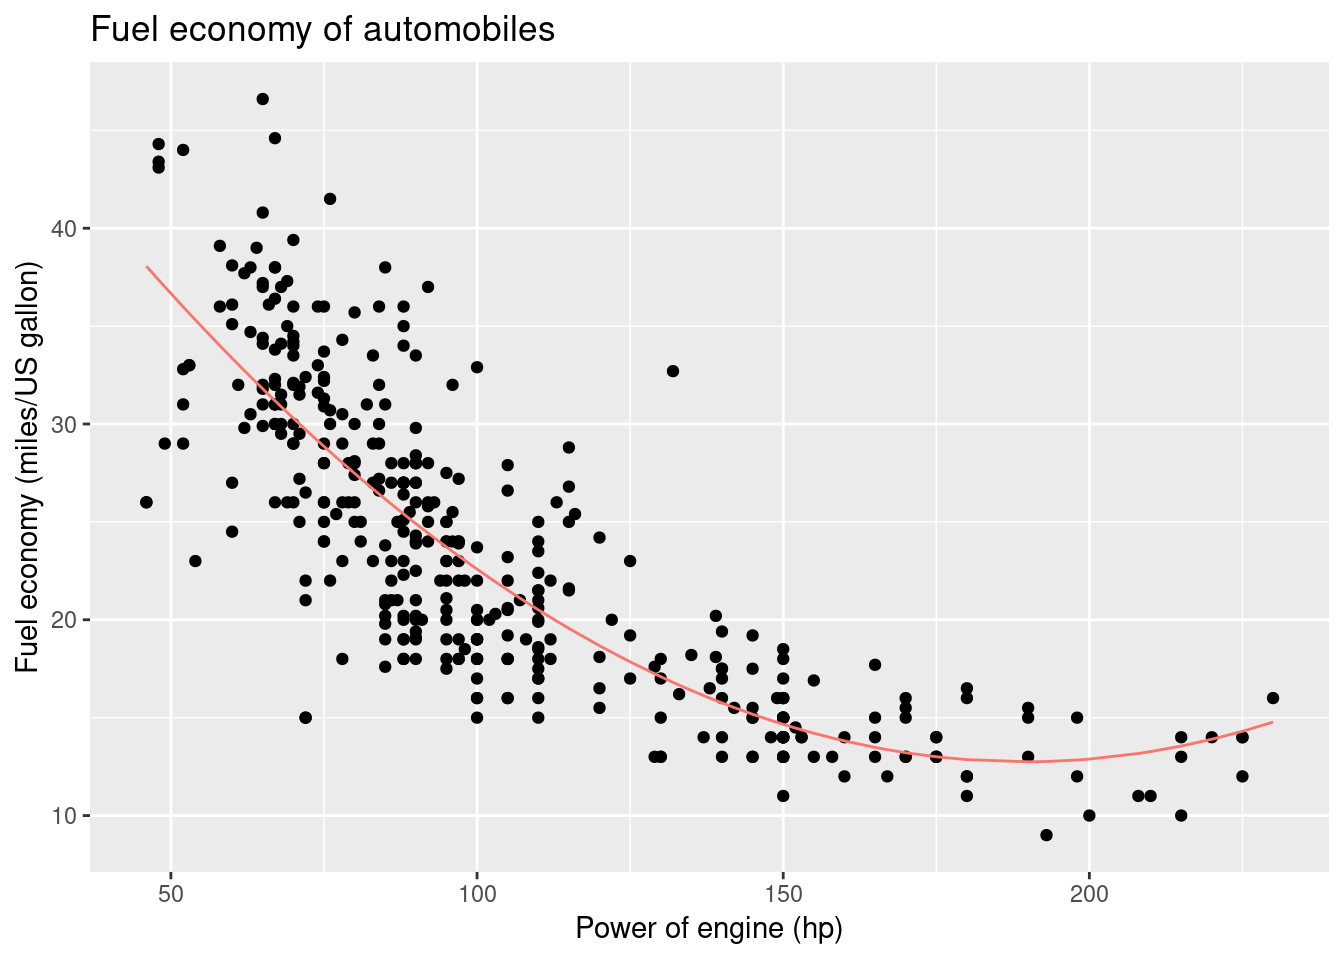
\includegraphics[width=0.7\linewidth]{LineaRModels_files/figure-latex/unnamed-chunk-8-1} \end{center}

This quadratic curve is nothing like an hyperplane! Let \(\boldsymbol{y} \equiv \texttt{mpg}\), \(\mathsf{x} = \texttt{hp}\) and \(\mathsf{z} = \texttt{hp}^2\). But recall that we are working in three dimensions (the intercept gives the height of the hyperplane) and the coordinates of our hyperplane are\\
\[\beta_0 + \beta_1x-y +\beta_2z =0.\]
However, the observations will always be such that \(z = x^2\), so our fitted values will lie on a one-dimensional subspace of this hyperplane.

The following 3D depiction hopefully captures this better and shows the fitted hyperplane along with the line on which all the (\(x_i, z_i\)) observations lie.

\begin{center}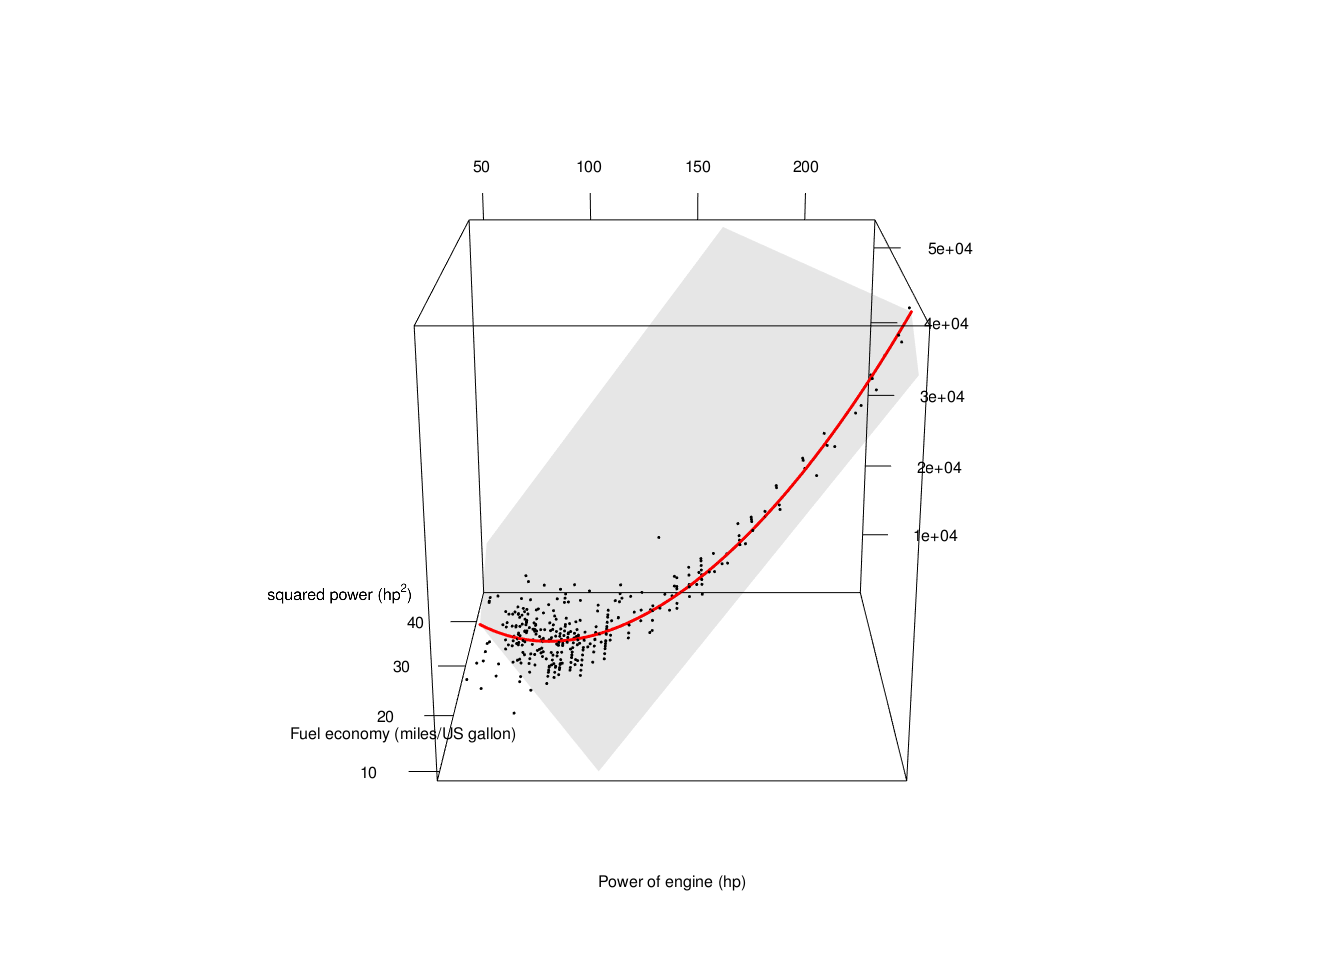
\includegraphics[width=0.7\linewidth]{LineaRModels_files/figure-latex/hyperplane-1} \end{center}

\hypertarget{centered-coefficient-of-determination}{%
\section{(Centered) coefficient of determination}\label{centered-coefficient-of-determination}}

Recall the decomposition of observations into fitted and residual vectors,
\[\boldsymbol{y} = (\boldsymbol{y} - \mathbf{X}\hat{\boldsymbol{\beta}}) + \mathbf{X}\hat{\boldsymbol{\beta}}= \boldsymbol{e} + \hat{\boldsymbol{y}}\]
where \(\boldsymbol{e} \equiv \mathbf{M}_{\mathbf{X}}\boldsymbol{y} \perp \hat{\boldsymbol{y}} \equiv \mathbf{H}_{\mathbf{X}}\boldsymbol{y}\).

The centered coefficient of determination, \(R^2_c\) measures the proportion of variation explained by the centered fitted values relative to the centered observations, i.e.,
\[ R^2_c = \frac{\|\hat{\boldsymbol{y}}-\bar{y}\mathbf{1}_n\|^2}{\|\boldsymbol{y}-\bar{y}\mathbf{1}_n\|^2}=\frac{\|\hat{\boldsymbol{y}}\|^2-\|\bar{y}\mathbf{1}_n\|^2}{\|\boldsymbol{y}\|^2-\|\bar{y}\mathbf{1}_n\|^2}.\]
since the vectors \(\bar{y}\mathbf{1}_n \perp \hat{\boldsymbol{y}}-\bar{y}\mathbf{1}_n\).

Provided that \(\mathbf{1}_n \in \mathscr{S}(\mathbf{X})\), it is obvious that the fitted values \(\hat{\boldsymbol{y}}\) are invariant to linear transformations of the covariates \(\mathbf{X}\) (by which I mean you can transform the design matrix column by column, with \(\mathbf{x}_i \mapsto \alpha_i+\mathbf{x}_i\gamma_i\) for \(i=1, \ldots, p\)). Multiplicative changes in \(\boldsymbol{y}\) lead to an equivalent change in \(\boldsymbol{e}\) and \(\hat{\boldsymbol{y}}\). However, location-changes in \(\boldsymbol{y}\) are only reflected in \(\hat{\boldsymbol{y}}\) (they are absorbed by the intercept). This is why \(R^2\) is not invariant to location-changes in the response, since the ratio \(\|\hat{\boldsymbol{y}}\|^2/\|\boldsymbol{y}\|^2\) increases to 1 if \({\boldsymbol{y}}\mapsto {\boldsymbol{y}}+ a \mathbf{1}_n\).

This invariance is precisely the reason we dismissed \(R^2\). For example, a change of units from Farenheit to Celcius, viz.~\(T_c = 5 (T_F - 32)/9\), leads to different values of \(R^2\):

\begin{Shaded}
\begin{Highlighting}[]
\KeywordTok{data}\NormalTok{(aatemp, }\DataTypeTok{package =} \StringTok{"faraway"}\NormalTok{)}
\KeywordTok{plot}\NormalTok{(temp }\OperatorTok{~}\StringTok{ }\NormalTok{year, }\DataTypeTok{data =}\NormalTok{ aatemp, }\DataTypeTok{ylab =} \StringTok{"Temperature (in F)"}\NormalTok{, }\DataTypeTok{bty =} \StringTok{"l"}\NormalTok{)}
\CommentTok{#Form design matrix and two response vectors}
\NormalTok{yF <-}\StringTok{ }\NormalTok{aatemp}\OperatorTok{$}\NormalTok{temp}
\NormalTok{n <-}\StringTok{ }\KeywordTok{length}\NormalTok{(yF)}
\NormalTok{yC <-}\StringTok{ }\DecValTok{5}\OperatorTok{/}\DecValTok{9}\OperatorTok{*}\NormalTok{(aatemp}\OperatorTok{$}\NormalTok{temp }\OperatorTok{-}\StringTok{ }\DecValTok{32}\NormalTok{)}
\NormalTok{X <-}\StringTok{ }\KeywordTok{cbind}\NormalTok{(}\DecValTok{1}\NormalTok{, aatemp}\OperatorTok{$}\NormalTok{year)}
\CommentTok{# Obtain OLS coefficients and fitted values}
\NormalTok{XtX <-}\StringTok{ }\KeywordTok{solve}\NormalTok{(}\KeywordTok{crossprod}\NormalTok{(X))}
\NormalTok{beta_hat_F <-}\StringTok{ }\NormalTok{XtX }\OperatorTok\StringTok{ }\KeywordTok{crossprod}\NormalTok{(X, yF)}
\KeywordTok{abline}\NormalTok{(}\DataTypeTok{a =}\NormalTok{ beta_hat_F[}\DecValTok{1}\NormalTok{], }\DataTypeTok{b =}\NormalTok{ beta_hat_F[}\DecValTok{2}\NormalTok{])}
\end{Highlighting}
\end{Shaded}

\begin{center}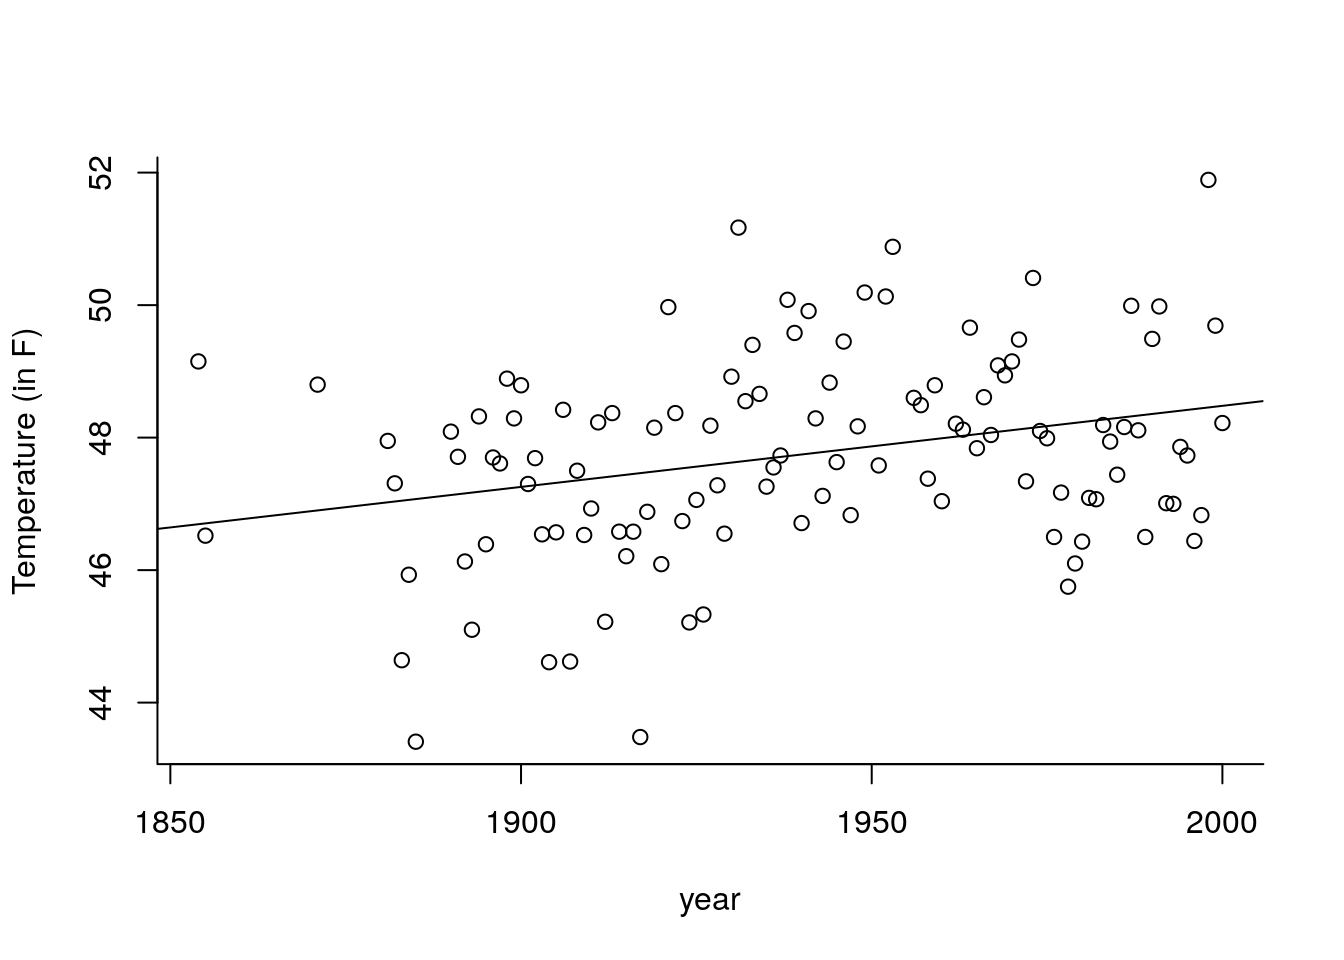
\includegraphics[width=0.7\linewidth]{LineaRModels_files/figure-latex/faraway-1} \end{center}

\begin{Shaded}
\begin{Highlighting}[]
\NormalTok{beta_hat_C <-}\StringTok{ }\NormalTok{XtX }\OperatorTok\StringTok{ }\KeywordTok{crossprod}\NormalTok{(X, yC)}
\NormalTok{fitted_F <-}\StringTok{ }\NormalTok{X }\OperatorTok\StringTok{ }\NormalTok{beta_hat_F}
\NormalTok{fitted_C <-}\StringTok{ }\NormalTok{X }\OperatorTok\StringTok{ }\NormalTok{beta_hat_C}
\CommentTok{# Compute coefficient of determination}
\NormalTok{R2_F <-}\StringTok{ }\KeywordTok{sum}\NormalTok{(fitted_F}\OperatorTok{^}\DecValTok{2}\NormalTok{)}\OperatorTok{/}\KeywordTok{sum}\NormalTok{(yF}\OperatorTok{^}\DecValTok{2}\NormalTok{)}
\NormalTok{R2_C <-}\StringTok{  }\KeywordTok{sum}\NormalTok{(fitted_C}\OperatorTok{^}\DecValTok{2}\NormalTok{)}\OperatorTok{/}\KeywordTok{sum}\NormalTok{(yC}\OperatorTok{^}\DecValTok{2}\NormalTok{)}
\CommentTok{#Centered R^2}
\NormalTok{R2c_F <-}\StringTok{ }\KeywordTok{sum}\NormalTok{((fitted_F}\OperatorTok{-}\KeywordTok{mean}\NormalTok{(yF))}\OperatorTok{^}\DecValTok{2}\NormalTok{)}\OperatorTok{/}\KeywordTok{sum}\NormalTok{((yF}\OperatorTok{-}\KeywordTok{mean}\NormalTok{(yF))}\OperatorTok{^}\DecValTok{2}\NormalTok{)}
\NormalTok{R2c_C <-}\StringTok{  }\KeywordTok{sum}\NormalTok{((fitted_C}\OperatorTok{-}\KeywordTok{mean}\NormalTok{(yC))}\OperatorTok{^}\DecValTok{2}\NormalTok{)}\OperatorTok{/}\KeywordTok{sum}\NormalTok{((yC}\OperatorTok{-}\KeywordTok{mean}\NormalTok{(yC))}\OperatorTok{^}\DecValTok{2}\NormalTok{)}
\KeywordTok{isTRUE}\NormalTok{(}\KeywordTok{all.equal}\NormalTok{(R2c_F, R2c_C))}
\end{Highlighting}
\end{Shaded}

\begin{verbatim}
## [1] TRUE
\end{verbatim}

The difference \(R^2(F)-R^2(C)=\) 0.00752 is small because the \(R^2\) value is very high, but the coefficient itself is also meaningless. In this example, \(R^2(F)=\) 0.9991, which seems to indicate excellent fit but in fact only 8.54\% of the variability is explained by year and we do an equally good job by simply taking \(\hat{y}_i=\bar{y}\).

\(R^2_c\) makes the comparison between the adjusted linear model and the null model with only a constant, which predicts each \(y_i (i=1, \ldots, n)\) by the average \(\bar{y}\).

If \(R^2_c\) gives a very rough overview of how much explanatory power \(\mathbf{X}\) has, it is not a panacea. If we add new covariates in \(\mathbf{X}\), the value of \(R^2_c\) necessarily increases. In the most extreme scenario, we could add a set of \(n-p\) linearly independent vectors to \(\mathbf{X}\) and form a new design matrix \(mX^*\) with those. The fitted values from running a regression with \(\mathbf{X}^*\) will be exactly equal to the observations \(\boldsymbol{y}\) and thus \(R^2_c=1\). However, I hope it is clear that this model will \emph{not} be useful. Overfitting leads to poor predictive performance; if we get a new set of \(\mathbf{x}_*\), we would predict the unobserved \(y_*\) using its conditional average \(\mathbf{x}_i^*\hat{\boldsymbol{\beta}}\) and this estimate will be rubish if we included too many meaningless covariates.

Other versions of \(R^2_c\) exist that include a penalty term for the number of covariates; these are not widely used and can be negative in extreme cases. We will cover better goodness-of-fit diagnostics later in the course.

\BeginKnitrBlock{rmdcaution}
In \textbf{R}, the function \texttt{lm} returns \(R^2_c\) by default (in the \texttt{summary} table, under the label \texttt{Multiple\ R-squared}. However, if you remove the intercept, you will get \(R^2\) without warning!
Contrast
\EndKnitrBlock{rmdcaution}

\begin{Shaded}
\begin{Highlighting}[]
\NormalTok{mod <-}\StringTok{ }\KeywordTok{lm}\NormalTok{(mpg }\OperatorTok{~}\StringTok{ }\NormalTok{horsepower, }\DataTypeTok{data =}\NormalTok{ Auto)}
\NormalTok{rsqc_lm <-}\StringTok{ }\KeywordTok{summary}\NormalTok{(mod)}\OperatorTok{$}\NormalTok{r.squared}
\CommentTok{#same model, now X = [1 horsepower] and y = mpg}
\NormalTok{X <-}\StringTok{ }\KeywordTok{cbind}\NormalTok{(}\DecValTok{1}\NormalTok{, Auto}\OperatorTok{$}\NormalTok{horsepower)}
\NormalTok{y <-}\StringTok{ }\NormalTok{Auto}\OperatorTok{$}\NormalTok{mpg}
\NormalTok{rsq_lm <-}\StringTok{ }\KeywordTok{summary}\NormalTok{(}\KeywordTok{lm}\NormalTok{(y }\OperatorTok{~}\StringTok{ }\NormalTok{X }\OperatorTok{-}\StringTok{ }\DecValTok{1}\NormalTok{))}\OperatorTok{$}\NormalTok{r.squared }

\CommentTok{#Compute quantities manually}
\NormalTok{rsqc_man <-}\StringTok{ }\KeywordTok{c}\NormalTok{(}\KeywordTok{crossprod}\NormalTok{(}\KeywordTok{fitted}\NormalTok{(mod) }\OperatorTok{-}\StringTok{ }\KeywordTok{mean}\NormalTok{(y)) }\OperatorTok{/}\StringTok{ }\KeywordTok{crossprod}\NormalTok{(y }\OperatorTok{-}\StringTok{ }\KeywordTok{mean}\NormalTok{(y)))}
\KeywordTok{isTRUE}\NormalTok{(}\KeywordTok{all.equal}\NormalTok{(rsqc_man, rsqc_lm))}
\end{Highlighting}
\end{Shaded}

\begin{verbatim}
## [1] TRUE
\end{verbatim}

\begin{Shaded}
\begin{Highlighting}[]
\NormalTok{rsq_man <-}\StringTok{ }\KeywordTok{c}\NormalTok{(}\KeywordTok{crossprod}\NormalTok{(}\KeywordTok{fitted}\NormalTok{(mod))}\OperatorTok{/}\KeywordTok{crossprod}\NormalTok{(y))}
\KeywordTok{isTRUE}\NormalTok{(}\KeywordTok{all.equal}\NormalTok{(rsq_man, rsq_lm))}
\end{Highlighting}
\end{Shaded}

\begin{verbatim}
## [1] TRUE
\end{verbatim}

\hypertarget{summary-of-week-2}{%
\section{Summary of week 2}\label{summary-of-week-2}}

If \(\mathbf{X}\) is an \(n \times p\) design matrix containing \emph{covariates} and \(\boldsymbol{Y}\) is our response variable, we can obtain the \emph{ordinary least squares} (OLS) coefficients for the linear model
\[\boldsymbol{y} = \mathbf{X}\boldsymbol{\beta}+ \boldsymbol{\varepsilon}, \qquad \mathrm{E}(\boldsymbol{\varepsilon})=\boldsymbol{0}_n,\]
by projecting \(\boldsymbol{y}\) on to \(\mathbf{X}\); it follows that
\[\mathbf{X}\hat{\boldsymbol{\beta}}=\mathbf{X}(\mathbf{X}^\top\mathbf{X})^{-1}\mathbf{X}^\top{\boldsymbol{y}}\] and
\[\hat{\boldsymbol{\beta}} = (\mathbf{X}^\top\mathbf{X})^{-1}\mathbf{X}^\top{\boldsymbol{y}}.\]

The dual interpretation (which is used for graphical diagnostics), is the row geometry: each row corresponds to an individual and the response is a \(1\) dimensional point.
\(\hat{\boldsymbol{\beta}}\) describes the parameters of the hyperplane that minimizes the sum of squared Euclidean vertical distances between the fitted value \(\hat{y}_i\) and the response \(y_i\).
The problem is best written using vector-matrix notation, so

\[ \mathrm{argmin}_{\boldsymbol{\beta}} \sum_{i=1}^n (y_i- \mathbf{x}_i\boldsymbol{\beta})^2 \equiv \mathrm{argmin}_{\boldsymbol{\beta}} (\boldsymbol{y} - \mathbf{X}\boldsymbol{\beta})^\top(\boldsymbol{y}-\mathbf{X}\boldsymbol{\beta}) \equiv \boldsymbol{e}^\top\boldsymbol{e}.
\]

The solution to the OLS problem has a dual interpretation in the column geometry, in which we treat the vector of stacked observations \((y_1, \ldots, y_n)^\top\) (respectively the vertical distances \((e_1, \ldots, e_n)^\top\)) as elements of \(\mathbb{R}^n\). There, the response \(\boldsymbol{y}\) space can be decomposed into \emph{fitted values} \(\hat{{\boldsymbol{y}}} \equiv \mathbf{H}_{\mathbf{X}} = \mathbf{X}\hat{\boldsymbol{\beta}}\) and \emph{residuals} \(\boldsymbol{e} = \mathbf{M}_{\mathbf{X}} = \boldsymbol{y} - \mathbf{X}\hat{\boldsymbol{\beta}}\). By construction, \(\boldsymbol{e} \perp \hat{{\boldsymbol{y}}}\).

We therefore get \[\boldsymbol{y} = \hat{\boldsymbol{y}} + \boldsymbol{e}\]
and since these form a right-angled triangle, Pythagoras' theorem can be used to show that
\(\|\boldsymbol{y}\|^2 = \|\hat{\boldsymbol{y}}\|^2 + \|\boldsymbol{e}\|^2.\)

\hypertarget{solutions-1}{%
\section{Solutions}\label{solutions-1}}

The following questions refer to the dataset \texttt{prostate} from the package \texttt{ElemStatLearn}.

\begin{enumerate}
\def\labelenumi{\alph{enumi}.}
\tightlist
\item
  Briefly describe the dataset.
\item
  Look at summaries of \texttt{lbph}. What likely value was imputed in places of zeros in `lbph\} (before taking the logarithm)?
\item
  Produce a plot of the pair of variables \texttt{lcavol} and \texttt{lpsa} on the log and on the original scale. Comment on the relationship between \texttt{lcavol} and \texttt{lpsa}.
\item
  Fit a linear model using the log cancer volume as response variable, including a constant and the log prostate specific antigen as covariates. Obtain numerically the OLS estimates \(\hat{\boldsymbol{\beta}}\) of the parameters, the fitted values \(\hat{\boldsymbol{y}}\) and the residuals \(\boldsymbol{e}\) using the formulas given in class.
\item
  Compare the quantities you obtained with the output of the function \texttt{lm}.
\item
  Add the fitted regression line to the scatterplot of \texttt{lcavol} against \texttt{lpsa}.
\item
  Interpret the changes in cancer volume (not the log cancer volume), including any units in your interpretations.
\item
  Obtain the orthogonal projection matrix \(\mathbf{H}_\mathbf{X}\) and the OLS coefficients \(\hat{\boldsymbol{\beta}}\) using a SVD decomposition of \(\mathbf{X}\) (\texttt{svd}).
\item
  Compute the \(R^2_c\) coefficient and compare with the one in \texttt{summary} output of the \texttt{lm} function. What can you say about the explanatory power of the covariate \texttt{lpsa}?
\end{enumerate}

\hypertarget{exercise-3.5---prostate-cancer}{%
\subsection{Exercise 3.5 - Prostate cancer}\label{exercise-3.5---prostate-cancer}}

The following questions refer to the dataset \texttt{prostate} from the package \texttt{ElemStatLearn}.

\begin{enumerate}
\def\labelenumi{\alph{enumi}.}
\tightlist
\item
  Briefly describe the data set.
\end{enumerate}

Running \texttt{?ElemStatLearn::prostate} gives the help file for the data set. Since we will be coming back to this example, detailed informations are provided below.

This data set was extracted from

\begin{quote}
Stamey, T.A., Kabalin, J.N., McNeal, J.E., Johnstone, I.M., Freiha, F., Redwine, E.A. and Yang, N. (1989)
Prostate specific antigen in the diagnosis and treatment of adenocarcinoma of the prostate: II. radical prostatectomy treated
patients, Journal of Urology 141(5), 1076--1083.
\end{quote}

This data set is described in Wakefield (2013), pp.~5-6.

\begin{quote}
The data were collected on \(n=97\) men before radical prostatectomy, a major surgical operation that
removes the entire prostate gland along with some surrounding tissue.
\end{quote}

\begin{quote}
In Stamey et al.~(1989), prostate specific antigen
(PSA) was proposed as a preoperative marker to predict the clinical stage of cancer. As well as modeling the stage of cancer as a
function of PSA, the authors also examined PSA as a function of age and seven other histological and morphometric covariates.
\end{quote}

\begin{quote}
The BPH and capsular penetration variables originally contained zeros, and a small number was substituted before the log transform was taken. It is not clear from the original paper why the log transform was taken though PSA varies over a wide range, and so linearity
of the mean model may be aided by the log transform. It is also not clear why the variable PGS45 was constructed.
\end{quote}

The data set contains the following variables:

\begin{itemize}
\tightlist
\item
  \texttt{lcavol}: log of cancer volume, measured in milliliters (cc). The area of cancer was measured from digitized images and
  multiplied by a thickness to produce a volume.
\item
  \texttt{lweight}: log of the prostate weight, measured in grams.
\item
  \texttt{age}: The age of the patient, in years.
\item
  \texttt{lbph}: log of the amount of benign prostatic hyperplasia (BPH), a noncancerous enlargement of the prostate gland, as
  an area in a digitized image and reported in cm\({}^2\).
\item
  \texttt{svi}: seminal vesicle invasion, a 0/1 indicator of whether prostate cancer cells have invaded the seminal vesicle.
\item
  \texttt{lcp}: log of the capsular penetration, which represents the level of extension of cancer into the capsule (the fibrous
  tissue which acts as an outer lining of the prostate gland), measured as the linear extent of penetration, in cm.
\item
  \texttt{gleason}: Gleason score, a measure of the degree of aggressiveness of the tumor. The Gleason grading system assigns a
  grade (1--5) to each of the two largest areas of cancer in the tissue samples with 1 being the least aggressive and 5 the most
  aggressive; the two grades are then added together to produce the Gleason score.
\item
  \texttt{pgg45}: percentage of Gleason scores that are 4 or 5.
\item
  \texttt{lpsa}: log of prostate specific antigen (PSA), a concentration measured in ng/m
\end{itemize}

To load the data set, use

\begin{Shaded}
\begin{Highlighting}[]
\CommentTok{#Install package if you get an error message}
\CommentTok{#install.packages("ElemStatLearn")}
\KeywordTok{data}\NormalTok{(prostate, }\DataTypeTok{package =} \StringTok{"ElemStatLearn"}\NormalTok{)}
\NormalTok{?ElemStatLearn}\OperatorTok{::}\NormalTok{prostate}
\KeywordTok{attach}\NormalTok{(prostate) }
\end{Highlighting}
\end{Shaded}

The command \texttt{attach} allows you to access column (variables) without using \texttt{\$} by adding the columns of the data frame to your work environment. \textbf{Always} detach the data once you are done with your analysis to avoid overriding or hidding variables.

\begin{enumerate}
\def\labelenumi{\alph{enumi}.}
\setcounter{enumi}{1}
\tightlist
\item
  Look at summaries of \texttt{lbph}. What likely value was imputed in places of zeros in \texttt{lbph} (before taking the logarithm)?
\end{enumerate}

\begin{Shaded}
\begin{Highlighting}[]
\NormalTok{bph <-}\StringTok{ }\KeywordTok{exp}\NormalTok{(lbph) }
\KeywordTok{head}\NormalTok{(bph) }\CommentTok{#look up first elements}
\end{Highlighting}
\end{Shaded}

\begin{verbatim}
## [1] 0.25 0.25 0.25 0.25 0.25 0.25
\end{verbatim}

\begin{Shaded}
\begin{Highlighting}[]
\KeywordTok{min}\NormalTok{(bph) }\CommentTok{#return minimum}
\end{Highlighting}
\end{Shaded}

\begin{verbatim}
## [1] 0.25
\end{verbatim}

\begin{Shaded}
\begin{Highlighting}[]
\KeywordTok{hist}\NormalTok{(bph, }\DataTypeTok{main =} \StringTok{"Histogram"}\NormalTok{, }\DataTypeTok{xlab =} \StringTok{"benign prostatic hyperplasia"}\NormalTok{)}
\KeywordTok{rug}\NormalTok{(bph) }
\end{Highlighting}
\end{Shaded}

\begin{center}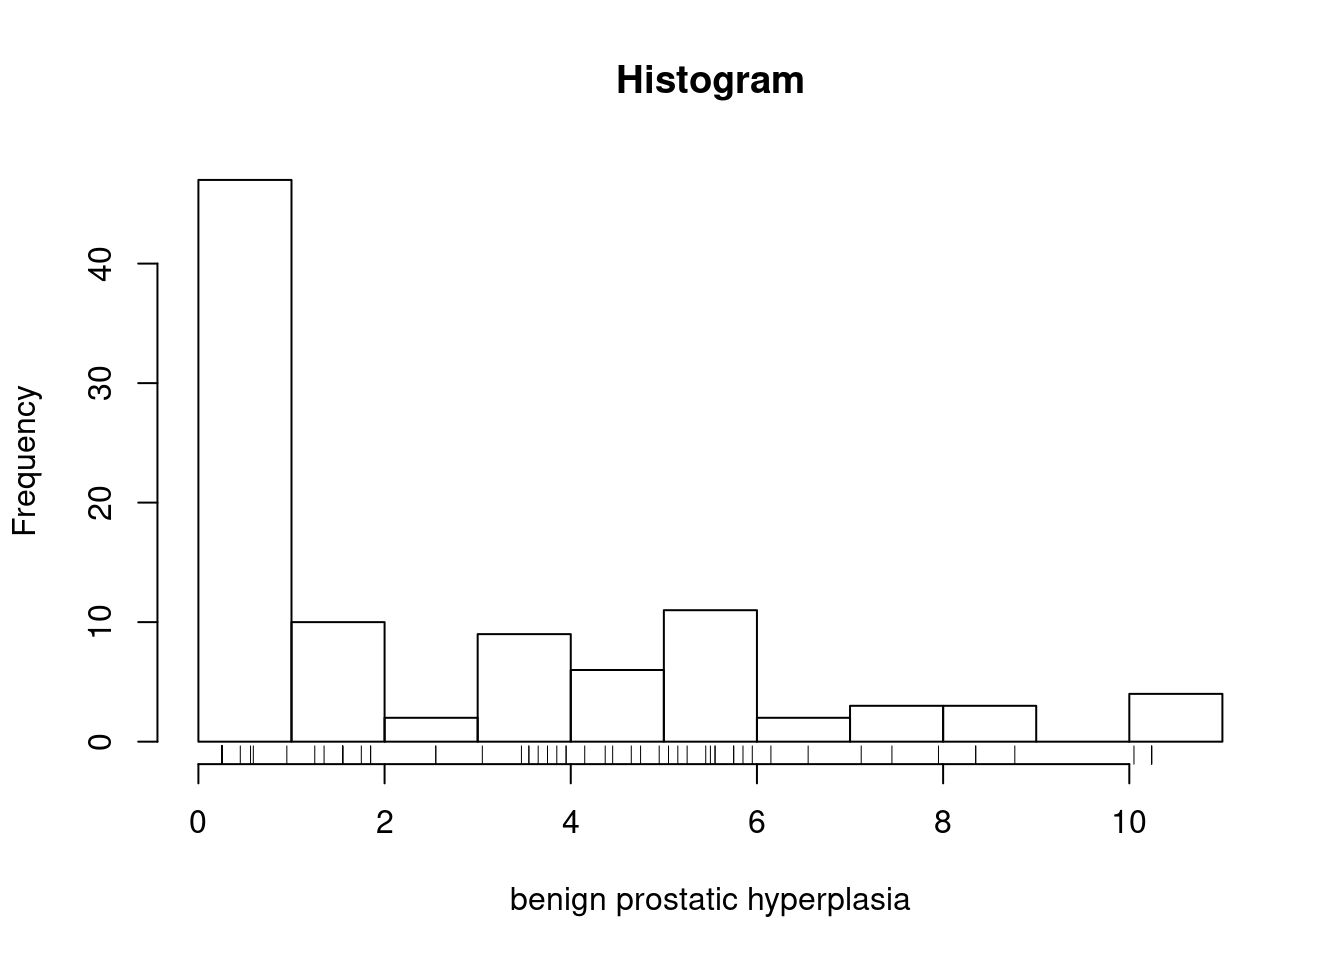
\includegraphics[width=0.7\linewidth]{LineaRModels_files/figure-latex/prostate_question_b2-1} \end{center}

\begin{Shaded}
\begin{Highlighting}[]
\CommentTok{#histogram, with lines below where the observations are}
\end{Highlighting}
\end{Shaded}

It seems likely that in order to take a logarithm, zeros were changed to 0.25. As such, we have to be careful with the interpretation of this coefficient if we include \texttt{bph} in the regression.

\begin{enumerate}
\def\labelenumi{\alph{enumi}.}
\setcounter{enumi}{1}
\tightlist
\item
  Produce a plot of the pair of variables \texttt{lcavol} and \texttt{lpsa} on the log and on the original scale. Comment on the relationship between \texttt{lcavol} and \texttt{lpsa}.
\end{enumerate}

\begin{Shaded}
\begin{Highlighting}[]
\KeywordTok{par}\NormalTok{(}\DataTypeTok{mfrow =} \KeywordTok{c}\NormalTok{(}\DecValTok{1}\NormalTok{, }\DecValTok{2}\NormalTok{)) }\CommentTok{#graphical parameters: two graphs per window}
\CommentTok{#Function plot is plot(x = , y = ) or plot(y ~ x)}
\CommentTok{#this works for vectors! (error message otherwise)}
\KeywordTok{plot}\NormalTok{(}\KeywordTok{exp}\NormalTok{(lpsa) }\OperatorTok{~}\StringTok{ }\KeywordTok{exp}\NormalTok{(lcavol),}
\DataTypeTok{xlab =} \StringTok{"Cancer volume (milliliters per cc)"}\NormalTok{, }\CommentTok{#y-axis label}
\DataTypeTok{ylab =} \StringTok{"prostate specific antigen (ng/ml)"}\NormalTok{, }\CommentTok{#x-axis label}
\DataTypeTok{main =} \StringTok{"Prostate cancer dataset"}\NormalTok{, }\CommentTok{#title}
\DataTypeTok{bty =} \StringTok{"l"}\NormalTok{, }\DataTypeTok{pch =} \DecValTok{20}\NormalTok{) }\CommentTok{#bty: remove box, only x-y axis}
\CommentTok{#pch: type of plotting symbol (small filled circle)}
\KeywordTok{plot}\NormalTok{(}\DataTypeTok{x =}\NormalTok{ lcavol, }\DataTypeTok{y =}\NormalTok{ lpsa,}
\DataTypeTok{xlab =} \StringTok{"cancer volume (milliliters per cc), log scale"}\NormalTok{,}
\DataTypeTok{ylab =} \StringTok{"prostate specific antigen (ng/ml), log scale"}\NormalTok{, }
\DataTypeTok{main =} \StringTok{"Prostate cancer dataset"}\NormalTok{,}
\DataTypeTok{bty =} \StringTok{"l"}\NormalTok{, }\DataTypeTok{pch =} \DecValTok{20}\NormalTok{)}

\KeywordTok{hist}\NormalTok{(}\KeywordTok{exp}\NormalTok{(lcavol), }\DataTypeTok{xlab =} \StringTok{"cancer volume (milliliters per cc)"}\NormalTok{, }\DataTypeTok{main =} \StringTok{"Histogram"}\NormalTok{)}
\KeywordTok{rug}\NormalTok{(}\KeywordTok{exp}\NormalTok{(lcavol))}
\KeywordTok{hist}\NormalTok{(}\KeywordTok{exp}\NormalTok{(lpsa), }\DataTypeTok{xlab =} \StringTok{"prostate specific antigen (ng/ml)"}\NormalTok{, }\DataTypeTok{main =} \StringTok{"Histogram"}\NormalTok{)}
\KeywordTok{rug}\NormalTok{(}\KeywordTok{exp}\NormalTok{(lpsa))}
\end{Highlighting}
\end{Shaded}

With \texttt{ggplot2}, the same graphs

\begin{Shaded}
\begin{Highlighting}[]
\KeywordTok{library}\NormalTok{(ggplot2)}

\KeywordTok{ggplot}\NormalTok{(}\DataTypeTok{data =}\NormalTok{ prostate, }\KeywordTok{aes}\NormalTok{(}\DataTypeTok{x =}\NormalTok{ lcavol, }\DataTypeTok{y =}\NormalTok{ lpsa)) }\OperatorTok{+}\StringTok{ }
\StringTok{  }\KeywordTok{geom_point}\NormalTok{() }\OperatorTok{+}
\StringTok{  }\KeywordTok{labs}\NormalTok{(}\DataTypeTok{y =} \StringTok{"prostate specific antigen (ng/ml), log scale"}\NormalTok{,}
       \DataTypeTok{x =} \StringTok{"cancer volume (milliliters per cc), log scale"}\NormalTok{,}
       \DataTypeTok{title =} \StringTok{"Prostate cancer dataset"}\NormalTok{)}
\end{Highlighting}
\end{Shaded}

\begin{center}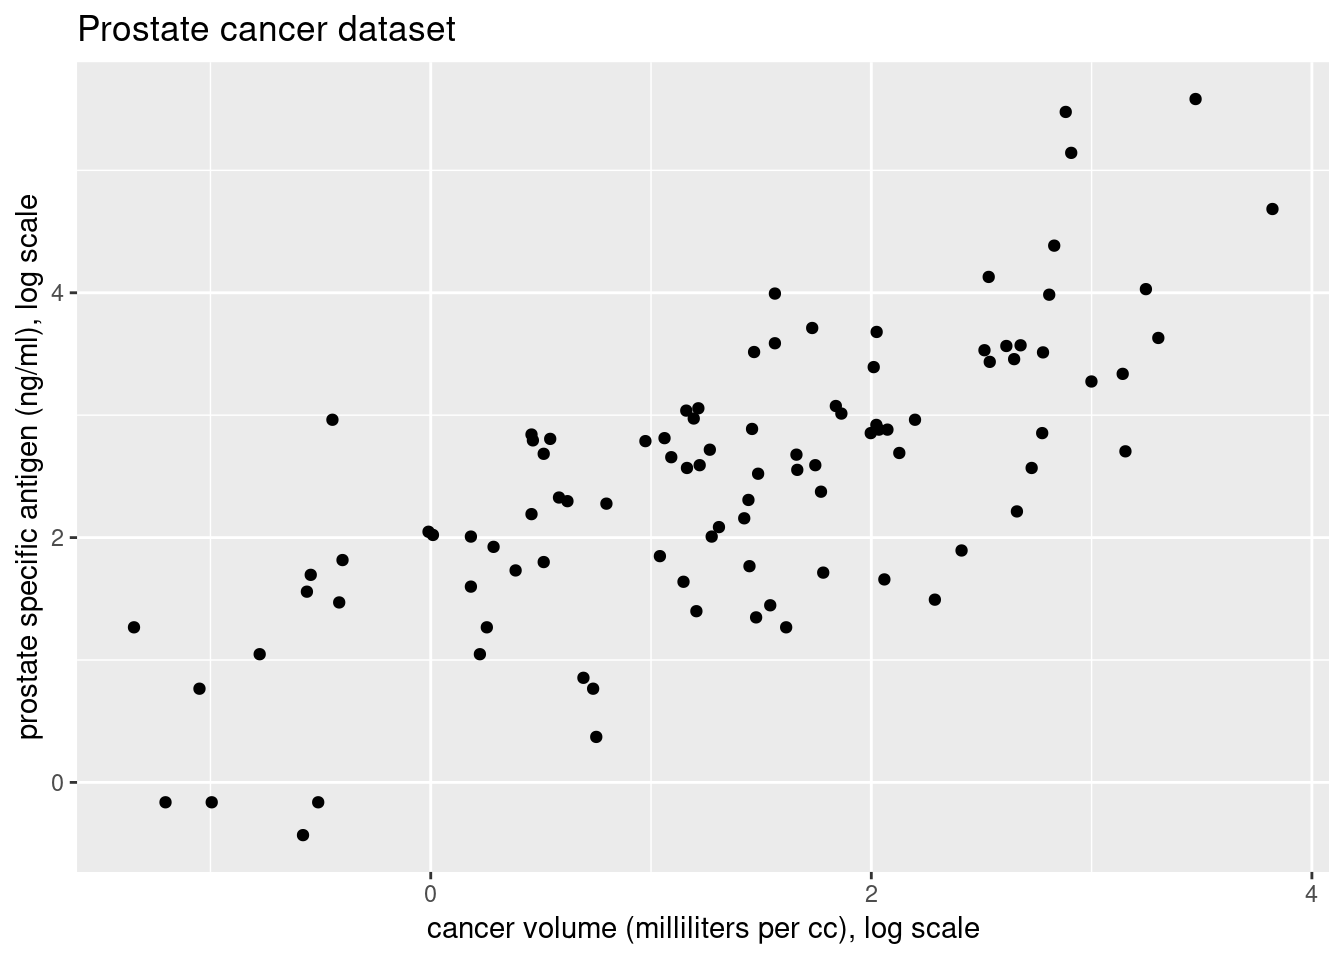
\includegraphics[width=0.7\linewidth]{LineaRModels_files/figure-latex/unnamed-chunk-11-1} \end{center}

\begin{Shaded}
\begin{Highlighting}[]
\KeywordTok{ggplot}\NormalTok{(}\DataTypeTok{data =}\NormalTok{ prostate, }\KeywordTok{aes}\NormalTok{(}\DataTypeTok{x =} \KeywordTok{exp}\NormalTok{(lcavol), }\DataTypeTok{y =} \KeywordTok{exp}\NormalTok{(lpsa))) }\OperatorTok{+}\StringTok{ }
\StringTok{  }\KeywordTok{geom_point}\NormalTok{() }\OperatorTok{+}
\StringTok{  }\KeywordTok{labs}\NormalTok{(}\DataTypeTok{y =} \StringTok{"prostate specific antigen (ng/ml)"}\NormalTok{,}
       \DataTypeTok{x =} \StringTok{"cancer volume (milliliters per cc)"}\NormalTok{,}
       \DataTypeTok{title =} \StringTok{"Prostate cancer dataset"}\NormalTok{)}
\end{Highlighting}
\end{Shaded}

\begin{center}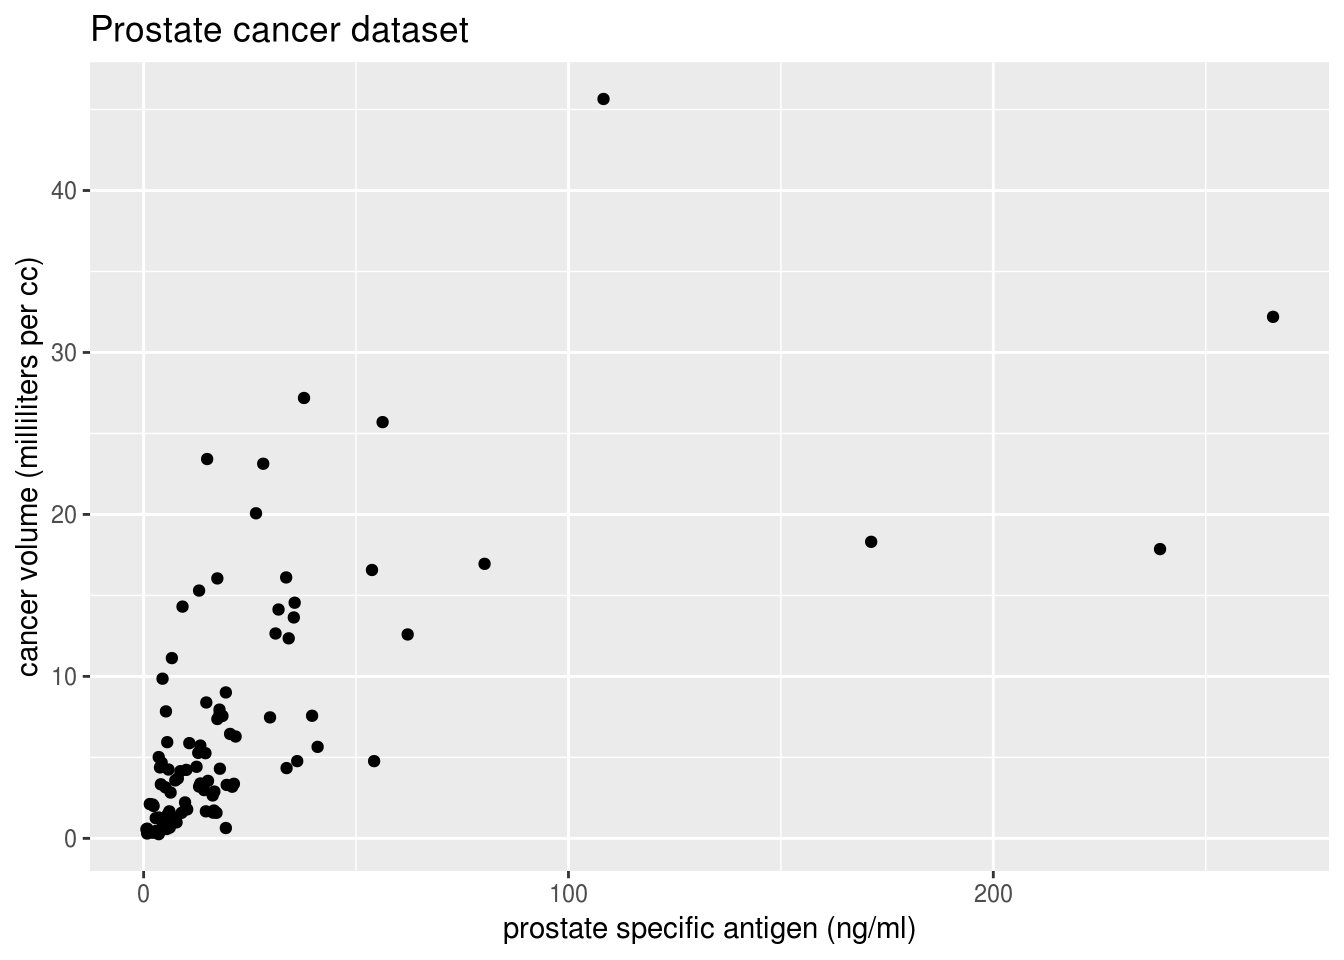
\includegraphics[width=0.7\linewidth]{LineaRModels_files/figure-latex/unnamed-chunk-11-2} \end{center}

\begin{Shaded}
\begin{Highlighting}[]
\KeywordTok{ggplot}\NormalTok{(}\DataTypeTok{data =}\NormalTok{ prostate, }\KeywordTok{aes}\NormalTok{(}\DataTypeTok{x =} \KeywordTok{exp}\NormalTok{(lcavol))) }\OperatorTok{+}\StringTok{ }
\StringTok{  }\KeywordTok{geom_histogram}\NormalTok{(}\DataTypeTok{bins =} \DecValTok{30}\NormalTok{) }\OperatorTok{+}\StringTok{ }\KeywordTok{geom_rug}\NormalTok{() }\OperatorTok{+}\StringTok{ }
\StringTok{  }\KeywordTok{labs}\NormalTok{(}\DataTypeTok{x =} \StringTok{"cancer volume (milliliters per cc)"}\NormalTok{,}
       \DataTypeTok{title =} \StringTok{"Histogram"}\NormalTok{)}
\end{Highlighting}
\end{Shaded}

\begin{center}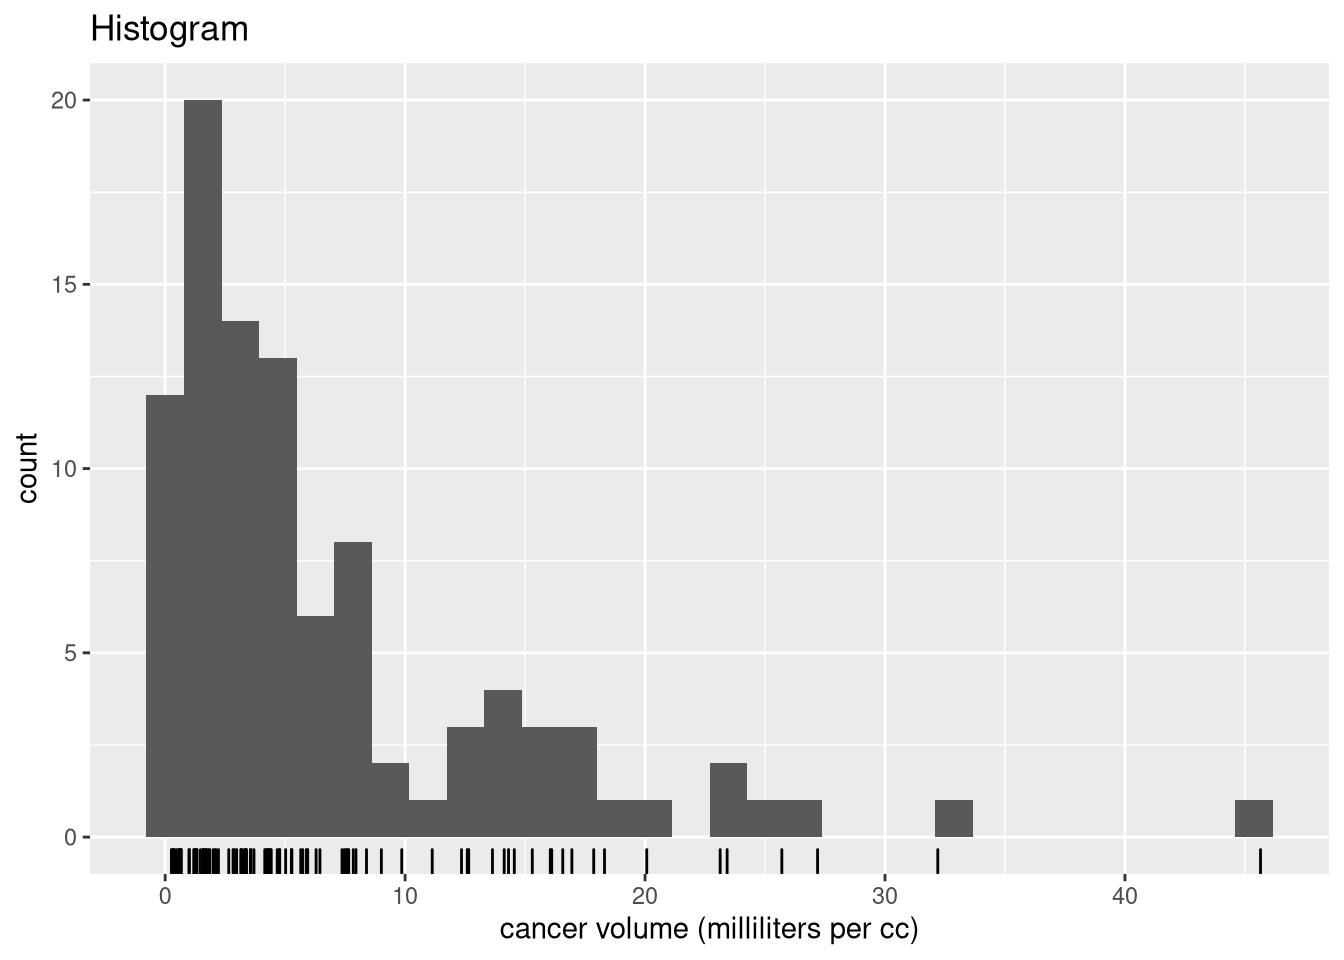
\includegraphics[width=0.7\linewidth]{LineaRModels_files/figure-latex/unnamed-chunk-11-3} \end{center}

We can see that both variables are positive and positively skewed, so a log transform may lead to a more linear relationship, as indicated by the pairs plot. A multiplicative model on the original scale is thus reasonable.

\begin{enumerate}
\def\labelenumi{\alph{enumi}.}
\setcounter{enumi}{3}
\tightlist
\item
  Fit a linear model using the log prostate specific antigen as response variable, including a constant and the log cancer volume as covariates. Obtain numerically the OLS estimates \(\hat{\boldsymbol{\beta}}\) of the parameters, the fitted values \(\hat{\boldsymbol{y}}\) and the residuals \(\boldsymbol{e}\) using the formulae given in class.
\end{enumerate}

\begin{Shaded}
\begin{Highlighting}[]
\NormalTok{fit <-}\StringTok{ }\KeywordTok{lm}\NormalTok{(lpsa }\OperatorTok{~}\StringTok{ }\NormalTok{lcavol, }\DataTypeTok{data =}\NormalTok{ prostate)}
\KeywordTok{summary}\NormalTok{(fit)}
\end{Highlighting}
\end{Shaded}

\begin{verbatim}
## 
## Call:
## lm(formula = lpsa ~ lcavol, data = prostate)
## 
## Residuals:
##      Min       1Q   Median       3Q      Max 
## -1.67624 -0.41648  0.09859  0.50709  1.89672 
## 
## Coefficients:
##             Estimate Std. Error t value Pr(>|t|)
## (Intercept)  1.50730    0.12194   12.36   <2e-16
## lcavol       0.71932    0.06819   10.55   <2e-16
## 
## Residual standard error: 0.7875 on 95 degrees of freedom
## Multiple R-squared:  0.5394, Adjusted R-squared:  0.5346 
## F-statistic: 111.3 on 1 and 95 DF,  p-value: < 2.2e-16
\end{verbatim}

\begin{Shaded}
\begin{Highlighting}[]
\CommentTok{#Create response vector and design matrix}
\NormalTok{y <-}\StringTok{ }\NormalTok{lpsa}
\NormalTok{X <-}\StringTok{ }\KeywordTok{cbind}\NormalTok{(}\DecValTok{1}\NormalTok{, lcavol)}
\CommentTok{#Create function to compute coefs "by hand"}
\NormalTok{coefs_vals <-}\StringTok{ }\ControlFlowTok{function}\NormalTok{(x, y)\{}
  \KeywordTok{c}\NormalTok{(}\KeywordTok{solve}\NormalTok{(}\KeywordTok{crossprod}\NormalTok{(x), }\KeywordTok{crossprod}\NormalTok{(x, y)))}
\NormalTok{\}}
\CommentTok{# Compute coefficients, fitted values and residuals}
\NormalTok{beta_hat <-}\StringTok{ }\KeywordTok{coefs_vals}\NormalTok{(}\DataTypeTok{x =}\NormalTok{ X, }\DataTypeTok{y =}\NormalTok{ lpsa)}
\NormalTok{yhat <-}\StringTok{ }\KeywordTok{c}\NormalTok{(X }\OperatorTok\StringTok{ }\NormalTok{beta_hat)}
\NormalTok{e <-}\StringTok{ }\NormalTok{y }\OperatorTok{-}\StringTok{ }\NormalTok{yhat}
\end{Highlighting}
\end{Shaded}

The function \texttt{lm} fits a linear model by least squares to a dataset. The function \texttt{summary} will return coefficient estimates, standard errors and various other statistics and print them in the console.

The formula for \texttt{lm} must be of the form \texttt{y\ \textasciitilde{}}, and any combination of the variables appearing on the right hand side of the \texttt{\textasciitilde{}} will be added as new columns of the design matrix. By default, the latter includes a column of ones. To remove it, use \texttt{+0} or \texttt{-1}. If you have two covariates \texttt{x1} and \texttt{x2}, the model \texttt{x1+x2} will have for \(i\)th row \((1, x_{i1}, x_{i2})\), while the model \texttt{x1+x2+x1:x2}\(\equiv\)\texttt{x1*x2} will include an \emph{interaction} term \texttt{x1:x2}. The latter just means product, so the \(i\)th row of the design matrix would be \((1, x_{i1}, x_{i2}, x_{i1}x_{i2})\). \textbf{R} will drop any collinear vectors, warn you and report \texttt{NA} in the summary output.

\begin{enumerate}
\def\labelenumi{\alph{enumi}.}
\setcounter{enumi}{4}
\tightlist
\item
  Compare the quantities you obtained in the last question with the output of the function \texttt{lm}.
\end{enumerate}

\begin{verbatim}
## [1] 1.5072975 0.7193204
\end{verbatim}

\begin{verbatim}
## (Intercept)      lcavol 
##   1.5072975   0.7193204
\end{verbatim}

\begin{verbatim}
## [1] TRUE
\end{verbatim}

\begin{verbatim}
## [1] TRUE
\end{verbatim}

\begin{verbatim}
## [1] TRUE
\end{verbatim}

\begin{enumerate}
\def\labelenumi{\alph{enumi}.}
\setcounter{enumi}{5}
\tightlist
\item
  Add the fitted regression line to the scatterplot of lcavol against lpsa .
\end{enumerate}

\begin{Shaded}
\begin{Highlighting}[]
\KeywordTok{par}\NormalTok{(}\DataTypeTok{mfrow =} \KeywordTok{c}\NormalTok{(}\DecValTok{1}\NormalTok{, }\DecValTok{1}\NormalTok{))}
\KeywordTok{plot}\NormalTok{(lpsa }\OperatorTok{~}\StringTok{ }\NormalTok{lcavol, }\DataTypeTok{data =}\NormalTok{ prostate,}
  \DataTypeTok{xlab =} \StringTok{"Cancer volume (milliliters per cc), log scale"}\NormalTok{,}
  \DataTypeTok{ylab =} \StringTok{"prostate specific antigen (ng/ml), log scale"}\NormalTok{, }
  \DataTypeTok{main =} \StringTok{"Prostate cancer dataset"}\NormalTok{,}
  \DataTypeTok{bty =} \StringTok{"l"}\NormalTok{, }\DataTypeTok{pch =} \DecValTok{20}\NormalTok{)}
\KeywordTok{abline}\NormalTok{(fit, }\DataTypeTok{lwd =} \DecValTok{2}\NormalTok{) }\CommentTok{#simply add regression line, lwd is line width}
\end{Highlighting}
\end{Shaded}

\begin{Shaded}
\begin{Highlighting}[]
\KeywordTok{ggplot}\NormalTok{(}\DataTypeTok{data =}\NormalTok{ prostate, }\KeywordTok{aes}\NormalTok{(}\DataTypeTok{x =}\NormalTok{ lcavol, }\DataTypeTok{y =}\NormalTok{ lpsa)) }\OperatorTok{+}\StringTok{ }
\StringTok{  }\KeywordTok{geom_point}\NormalTok{() }\OperatorTok{+}
\StringTok{  }\KeywordTok{labs}\NormalTok{(}\DataTypeTok{y =} \StringTok{"prostate specific antigen (ng/ml), log scale"}\NormalTok{,}
       \DataTypeTok{x =} \StringTok{"cancer volume (milliliters per cc), log scale"}\NormalTok{,}
       \DataTypeTok{title =} \StringTok{"Prostate cancer dataset"}\NormalTok{) }\OperatorTok{+}\StringTok{ }
\StringTok{  }\KeywordTok{geom_smooth}\NormalTok{(}\DataTypeTok{method =} \StringTok{"lm"}\NormalTok{, }\DataTypeTok{se =} \OtherTok{FALSE}\NormalTok{)}
\end{Highlighting}
\end{Shaded}

\begin{center}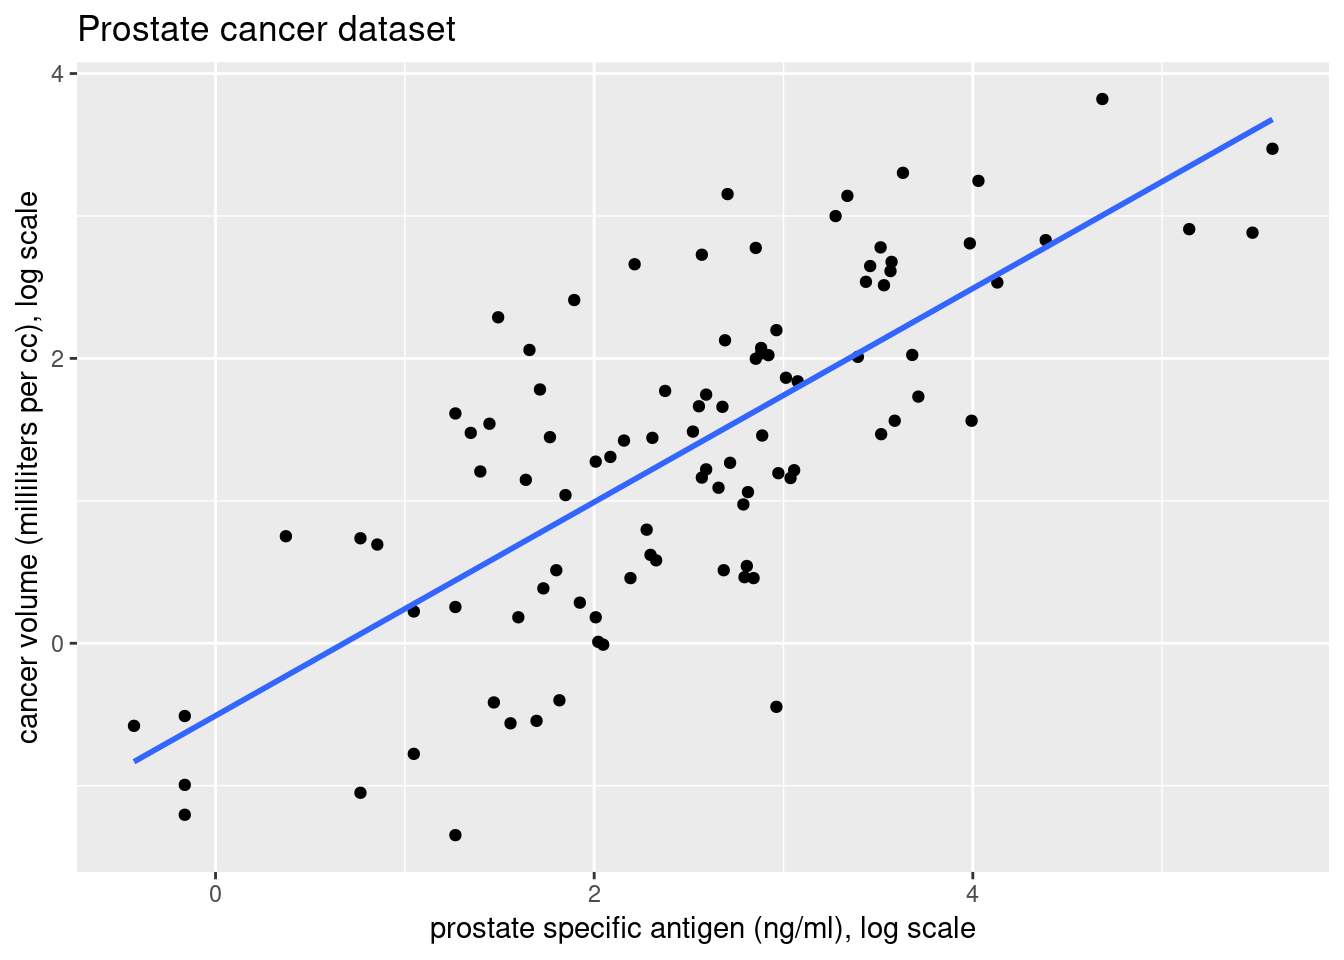
\includegraphics[width=0.7\linewidth]{LineaRModels_files/figure-latex/question_eggplot2-1} \end{center}

\begin{enumerate}
\def\labelenumi{\alph{enumi}.}
\setcounter{enumi}{6}
\tightlist
\item
  Interpret the changes in prostate specific antigen (not the log prostate specific antigen), including any units in your interpretations.
\end{enumerate}

The interpretation is as follows. We fit
\[\log(\texttt{psa}_i) = \beta_0 + \beta_1 \log(\texttt{cavol}_i) + \varepsilon_i.\]

On the original scale, this translates into the multiplicative model \(\texttt{psa}_i= \exp^{\beta_0}\texttt{cavol}_i^{\beta_1}\exp(\varepsilon_i)\).
The effect of an increase of the volume of cancer of prostate cancer by one milliliter per cubic centimeter depends on the size of the latter of \(\texttt{cavol}\), \((\texttt{cavol}_1/\texttt{cavol}_2)^{\beta_1}\) for levels \(\texttt{cavol}_1\) and \(\texttt{cavol}_2\).
For example, an increase of the cancer volume from 2 ml per cc to 3 ml per cc leads to an increase of the concentration of PSA of 1.34 ng/ml.

\begin{enumerate}
\def\labelenumi{\alph{enumi}.}
\setcounter{enumi}{7}
\tightlist
\item
  Using the results of Exercise 4.2, obtain the orthogonal projection matrix \(\mathbf{H}_{\mathbf{X}}\) and \(\hat{\boldsymbol{\beta}}\) using a SVD decomposition (\texttt{svd}). Check your output.
\end{enumerate}

\begin{Shaded}
\begin{Highlighting}[]
\CommentTok{#Hat matrix}
\NormalTok{Hmat <-}\StringTok{ }\NormalTok{X }\OperatorTok\StringTok{ }\KeywordTok{solve}\NormalTok{(}\KeywordTok{crossprod}\NormalTok{(X)) }\OperatorTok\StringTok{ }\KeywordTok{t}\NormalTok{(X)}
\CommentTok{#SVD decomposition of X}
\NormalTok{svdX <-}\StringTok{ }\KeywordTok{svd}\NormalTok{(X)}
\CommentTok{#OLS coefficients}
\NormalTok{beta_hat_svd <-}\StringTok{ }\NormalTok{svdX}\OperatorTok{$}\NormalTok{v }\OperatorTok\StringTok{ }\NormalTok{(}\KeywordTok{t}\NormalTok{(svdX}\OperatorTok{$}\NormalTok{u) }\OperatorTok\StringTok{ }\NormalTok{lpsa }\OperatorTok{/}\StringTok{ }\NormalTok{svdX}\OperatorTok{$}\NormalTok{d)}
\NormalTok{Hmat_svd <-}\StringTok{ }\KeywordTok{tcrossprod}\NormalTok{(svdX}\OperatorTok{$}\NormalTok{u)}
\CommentTok{#Check that both quantities are equal}
\KeywordTok{all.equal}\NormalTok{(Hmat, Hmat_svd, }\DataTypeTok{check.attributes =} \OtherTok{FALSE}\NormalTok{) }
\end{Highlighting}
\end{Shaded}

\begin{verbatim}
## [1] TRUE
\end{verbatim}

\begin{Shaded}
\begin{Highlighting}[]
\CommentTok{#use check.attributes = FALSE }
\CommentTok{#if you want to compare only the values}
\CommentTok{#and not e.g. the column names}
\KeywordTok{all.equal}\NormalTok{(}\KeywordTok{c}\NormalTok{(beta_hat_svd), beta_hat)}
\end{Highlighting}
\end{Shaded}

\begin{verbatim}
## [1] TRUE
\end{verbatim}

\begin{enumerate}
\def\labelenumi{\roman{enumi}.}
\tightlist
\item
  Compute the \(R^2_c\) coefficient and compare with the one in summary output of the \texttt{lm} function. What
  can you say about the explanatory power of the covariate \texttt{lpsa} ?
\end{enumerate}

\begin{Shaded}
\begin{Highlighting}[]
\NormalTok{R2c <-}\StringTok{ }\KeywordTok{sum}\NormalTok{((yhat}\OperatorTok{-}\KeywordTok{mean}\NormalTok{(y))}\OperatorTok{^}\DecValTok{2}\NormalTok{)}\OperatorTok{/}\KeywordTok{sum}\NormalTok{((y}\OperatorTok{-}\KeywordTok{mean}\NormalTok{(y))}\OperatorTok{^}\DecValTok{2}\NormalTok{)}
\NormalTok{R2c_lm <-}\StringTok{ }\KeywordTok{summary}\NormalTok{(fit)}\OperatorTok{$}\NormalTok{r.squared }\CommentTok{#this is centered version}
\KeywordTok{all.equal}\NormalTok{(R2c, R2c_lm)}
\end{Highlighting}
\end{Shaded}

\begin{verbatim}
## [1] TRUE
\end{verbatim}

\begin{Shaded}
\begin{Highlighting}[]
\CommentTok{#Detach prostate from environment}
\KeywordTok{detach}\NormalTok{(prostate)}
\end{Highlighting}
\end{Shaded}

The value of \(R^2_c\) is about 0.54, so about half the variability can be explained by the model. There is reasonable explanatory power. Note that presence of cancer causes the prostate specific antigens to increase (not the other way around!). A linear model could nevertheless be sensible here if we wished to obtain a non-invasive detector for predicting presence/absence of cancer, assuming the antigen is present in blood samples, but that detection of cancer would require otherwise a biopsy.

\begin{enumerate}
\def\labelenumi{\alph{enumi}.}
\setcounter{enumi}{9}
\tightlist
\item
  Perform an explanatory data analysis of the \texttt{prostate} data set. Summarize your findings.
\end{enumerate}

Here are some of the most important features we could detect by looking at the description, plots and summaries of the data set.

\begin{itemize}
\tightlist
\item
  Goal of the study: ``PSA was proposed as a preoperative marker to predict the clinical stage of cancer'';
\item
  Individuals in the data set form a subset of the population of the study; the subset consists of men about to undergo radical prostatectomy. This implies they are in late stages of prostate cancer (see \texttt{gleason});
\item
  No missing values, no obvious outlier;
\item
  Many variables are given on the log scale, potentially to remove the skewness (\texttt{lcavol}, \texttt{lweight}, \texttt{lcp}, \texttt{lbph}). This makes sense for volume (why?), less so for other variables;
\item
  The most relevant explanatory variables are cancer volume (\texttt{lcavol}), weight (\texttt{lweight}) and SVI (\texttt{svi});
\item
  It is not clear why and how \texttt{pgg45} was constructed;
\item
  0.25 was added to benign prostatic hyperplasia and capsular penetration before taking the log-transform (to get \texttt{lbph} and \texttt{lcp}). It would perhaps be more adequate for interpretability to transform the capsular penetration back to the original scale;
\item
  The weight of the tumor (\texttt{lweight}) is correlated with benign prostatic hyperplasia (consider an interaction term);
\item
  Gleason is an ordered categorical, so it makes sense to cast it to a factor, with categories 6, 7 and (8,9). The seminal vesicle invasion (\texttt{svi}) is already binary;
\item
  Obs. 37 is the only one with a Gleason score of 8 --- keeping it leads to perfect fit for this data point and will lead to problems with cross-validation if \texttt{gleason} is included as a factor in the mean model;
\end{itemize}

Note that we cannot say anything about the distribution of the response \texttt{exp(lpsa)}, because the Gaussian linear model assumes the mean is \(\mathbf{X}\boldsymbol{\beta}\) (so the skewness could be removed through the inclusion of covariates). Rather, one could fit both models on \texttt{exp(lpsa)} and \texttt{lpsa} scale and compare the diagnostics for the residuals.

\hypertarget{frischwaughlovell-theorem}{%
\chapter{Frisch--Waugh--Lovell theorem}\label{frischwaughlovell-theorem}}

The FWL theorem has two components: it gives a formula for partitioned OLS estimates and shows that residuals from sequential regressions are identical.

Consider the following linear regression
\[
 {\boldsymbol{y}}= \mathbf{X}_1\boldsymbol{\beta}_1+\mathbf{X}_2\boldsymbol{\beta}_2+ \boldsymbol{u}, \label{eq1}
\]
where the response vector \({\boldsymbol{y}}\) is \(n \times 1\), the vector of errors \(\boldsymbol{u}\) is a realization from a mean zero random
variable. The \(n \times p\) full-rank design matrix \(\mathbf{X}\) can be written as the partitioned
matrix \((\mathbf{X}_1^\top, \mathbf{X}_2^\top)^\top\) with blocks \(\mathbf{X}_1\), an \(n \times p_1\) matrix, and \(\mathbf{X}_2\), an \(n \times p_2\) matrix. Let
\(\hat{\boldsymbol{\beta}}_1\)
and \(\hat{\boldsymbol{\beta}}_2\) be the ordinary
least square (OLS) parameter estimates from running this regression. Define the orthogonal projection matrix \(\mathbf{H}_\mathbf{X}\) as usual and
\(\mathbf{H}_{\mathbf{X}_i} = \mathbf{X}_i(\mathbf{X}_i^\top\mathbf{X}_i)^{-1}\mathbf{X}_i^\top\) for \(i=1, 2\). Similarly,
define the complementary projection matrices \(\mathbf{M}_{\mathbf{X}_1}=\mathbf{I}_n-\mathbf{H}_{\mathbf{X}_1}\) and \(\mathbf{M}_{\mathbf{X}_2}=\mathbf{I}_n-\mathbf{H}_{\mathbf{X}_2}\).

\BeginKnitrBlock{theorem}
\protect\hypertarget{thm:unnamed-chunk-13}{}{\label{thm:unnamed-chunk-13} }The ordinary least square estimates of \(\boldsymbol{\beta}_2\) and the residuals from \eqref{eq1} are identical to those obtained by
running the regression
\[
 \mathbf{M}_{\mathbf{X}_1}{\boldsymbol{y}}= \mathbf{M}_{\mathbf{X}_1}\mathbf{X}_2\boldsymbol{\beta}_2 + \text{residuals}. \label{eq2} \
\]
\EndKnitrBlock{theorem}

\BeginKnitrBlock{rmdcaution}
In general, premultiplying both sides of the regression model by a projection matrix alters the model, so you will get different fitted values and residuals. Similarly, the model
\[\boldsymbol{Y} = \mathbf{X}_1 \boldsymbol{\beta}_1 + \mathbf{X}_2\boldsymbol{\beta}_2 + \boldsymbol{\varepsilon}\]
is \textbf{not} equivalent to
\[
\mathbf{M}_{\mathbf{X}_1}\boldsymbol{y} = \mathbf{M}_{\mathbf{X}_1}\mathbf{X}_2 \boldsymbol{\beta}_2 + \mathbf{M}_{\mathbf{X}_1}\boldsymbol{\varepsilon}
\]
because \(\boldsymbol{\varepsilon}\) is not in \(\mathbf{M}_\mathbf{X}\). This is true for the orthogonal decomposition
\[
\mathbf{M}_{\mathbf{X}_1}\boldsymbol{y} = \mathbf{M}_{\mathbf{X}_1}\mathbf{X}_2 \hat{\boldsymbol{\beta}}_2 + \mathbf{M}_{\mathbf{X}_1}\boldsymbol{e}
\]
\EndKnitrBlock{rmdcaution}

Below is an algebraic proof of the equality of the OLS coefficients. The following material is \textbf{optional}.

\BeginKnitrBlock{proof}
\iffalse{} {Proof. } \fi{}The easiest proof uses projection matrices, but we demonstrate the result for OLS coefficients directly.
Consider an invertible \(d \times d\) matrix \(\mathbf{C}\) and denote its inverse by \(\mathbf{D}\); then
\[
\begin{pmatrix} \mathbf{C}_{11} & \mathbf{C}_{12} \\ \mathbf{C}_{21} &\mathbf{C}_{22}
\end{pmatrix}\begin{pmatrix} \mathbf{D}_{11} & \mathbf{D}_{12} \\ \mathbf{D}_{21} &\mathbf{D}_{22}
\end{pmatrix}
=\mathbf{I}_p
\]
gives the relationships
\begin{align*}
\mathbf{C}_{11}\mathbf{D}_{11}+\mathbf{C}_{12}\mathbf{D}_{21} &= \mathbf{I}_{p_1}\\
\mathbf{C}_{11}\mathbf{D}_{12}+\mathbf{C}_{12}\mathbf{D}_{22} &= \mathbf{O}_{p_1, p_2}\\
\mathbf{C}_{22}\mathbf{D}_{21}+\mathbf{C}_{21}\mathbf{D}_{11} &= \mathbf{O}_{p_2, p_1}\\
\mathbf{C}_{22}\mathbf{D}_{22}+\mathbf{C}_{21}\mathbf{D}_{12} &= \mathbf{I}_{p_2}\\
\end{align*}
from which we deduce that the so-called Schur complement of \(\mathbf{C}_{22}\) is \[\mathbf{C}_{11}+\mathbf{C}_{12}\mathbf{C}^{-1}_{22}\mathbf{C}_{21} = \mathbf{D}_{11}^{-1}\]
and
\[
-\mathbf{C}_{22}\mathbf{C}_{21}(\mathbf{C}_{11}+\mathbf{C}_{12}\mathbf{C}^{-1}_{22}\mathbf{C}_{21})^{-1} = \mathbf{D}_{21}.
\]
Substituting
\[
\begin{pmatrix} \mathbf{C}_{11} & \mathbf{C}_{12} \\ \mathbf{C}_{21} &\mathbf{C}_{22}
\end{pmatrix} \equiv \begin{pmatrix} \mathbf{X}_1^\top\mathbf{X}_1 & \mathbf{X}_1^\top\mathbf{X}_2\\\mathbf{X}_2^\top\mathbf{X}_1  &\mathbf{X}_2^\top\mathbf{X}_2 
\end{pmatrix}
\]
and plug-in this result back in the equation for the least squares yields
\begin{align*}
\hat{\boldsymbol{\beta}}_1 &= (\mathbf{D}_{11}\mathbf{X}_1^\top + \mathbf{D}_{12}\mathbf{X}_2^\top)\boldsymbol{y} 
\\&= \mathbf{D}_{11}( \mathbf{X}_1^\top - \mathbf{C}_{12}\mathbf{C}_{22}^{-1}\mathbf{X}_2)\boldsymbol{y}
\\&= \left(\mathbf{C}_{11}+\mathbf{C}_{12}\mathbf{C}^{-1}_{22}\mathbf{C}_{21}\right)^{-1} \mathbf{X}_1^\top\mathbf{M}_{\mathbf{X}_2}\boldsymbol{y} 
\\&= (\mathbf{X}_1^\top\mathbf{M}_{\mathbf{X}_2}\mathbf{X}_1)^{-1}\mathbf{X}_1^\top\mathbf{M}_{\mathbf{X}_2}\boldsymbol{y}.
\end{align*}

The proof that the residuals are the same is left as an exercise.
\EndKnitrBlock{proof}

The Frisch--Waugh--Lovell theorem dates back to the work of \href{https://www.jstor.org/stable/1907330}{Frisch, R. and F. Waugh (1933)} and of \href{https://doi.org/10.1080/01621459.1963.10480682}{M. Lovell (1963)}.

\hypertarget{revisiting-the-interpretation-of-the-parameters-of-a-linear-model}{%
\section{Revisiting the interpretation of the parameters of a linear model}\label{revisiting-the-interpretation-of-the-parameters-of-a-linear-model}}

Geometrically, the linear model \(\boldsymbol{y} = \mathbf{X} \boldsymbol{\beta} + \text{residuals}\) corresponds to the projection on to the span of \(\mathbf{X}\) and gives the line of best fit in that space.

It is perhaps easiest to visualize the two-dimensional case, when \(\mathbf{X} = (\mathbf{1}_n^\top, \mathbf{x}_1^\top)^\top\) is a \(n \times 2\) design matrix and \(\mathbf{x}_1\) is a continuous covariate. In this case, the coefficient vector \(\boldsymbol{\beta}=(\beta_0, \beta_1)^\top\) represent, respectively, the intercept and the slope.

If \(\mathbf{X} = \mathbf{1}_n\), the model only consists of an intercept, which is interpreted as the mean level. Indeed, the projection matrix corresponding to \(\mathbf{1}_n\), \(\mathbf{H}_{\mathbf{1}_n}\), is a matrix whose entries are all identically \(n^{-1}\). The fitted values of this model thus correspond to the mean of \(\boldsymbol{y}\), \(\bar{y}\) and the residuals are the centred values \(\boldsymbol{y}-\mathbf{1}_n \bar{y}\) whose mean is zero.

More generally, for \(\mathbf{X}\) an \(n \times p\) design matrix, the interpretation is as follows: a unit increase in \(\mathrm{x}_{ij}\) (\(\mathrm{x}_{ij} \mapsto \mathrm{x}_{ij}+1)\) leads to a change of \(\beta_j\) unit for \(y_i\) (\(y_i \mapsto \beta_j+y_i\)), other things being held constant. Beware of models with higher order polynomials and interactions: if for example one is interested in the coefficient for \(\mathbf{x}_j\), but \(\mathbf{x}_j^2\) is also a column of the design matrix, then a change of one unit in \(\mathbf{x}_j\) will not lead to a change of \(\beta_jx_j\) for \(y_j\)!

The FWL theorem says the coefficient \(\boldsymbol{\beta}_2\) in the regression
\[\boldsymbol{y} =\mathbf{X}_1\boldsymbol{\beta}_1 + \mathbf{X}_2\boldsymbol{\beta}_2 + \boldsymbol{\varepsilon}\] is equivalent to that of the regression
\[\mathbf{M}_1\boldsymbol{y} =\mathbf{M}_1 \mathbf{X}_2\boldsymbol{\beta}_2 + \boldsymbol{\varepsilon} \]
This can be useful to distangle the effect of one variable.

The intercept coefficient does not correspond to the mean of \(\boldsymbol{y}\) unless the other variables in the design matrix have been centered (meaning they have mean zero). Otherwise, the coefficient \(\beta_0\) associated to the intercept is nothing but the level of \(y\) when all the other variables are set to zero.
Adding new variables affects the estimates of the coefficient vector \(\boldsymbol{\beta}\), unless the new variables are orthogonal to the existing lot.

\hypertarget{factors}{%
\section{Factors}\label{factors}}

Oftentimes, the regressors that are part of the design matrix will be categorical variables, which can be ordered or unordered. In the design matrix, these will appear as matrix of binary indicators. In \textbf{R}, dummy variables (vectors of class \texttt{factor}) are used to indicate categorical variables, which are often encoded as strings or (perhaps worse) integers. The function \texttt{read.table} has an argument, \texttt{stringsAsFactors}, that will automatically cast strings to factors. Oftentimes, dummy indicators are encoded as integer vectors in data frames. There is a risk that the vector be interpreted as a continuous numeric if the levels are integers (for example, advancement of the state of an illness that is encoded as 1, 2, 3, \ldots).

Useful functions to deal with factors include

\begin{itemize}
\tightlist
\item
  \texttt{as.factor}: casts column vectors to factors;\\
\item
  \texttt{is.factor}: to check whether the vector is a factor;
\item
  \texttt{class}: reports the encoding (\texttt{factor} for factor objects);
\item
  \texttt{summary}: displays counts of the various levels of a factor in place of the usual summary statistics;
\item
  \texttt{levels}: the names of the different levels of a factor; can be used to replace existing category names by more meaningful ones;
\end{itemize}

The function \texttt{lm} knows how to deal with \texttt{factor} objects and will automatically transform it to a matrix of binary indiactors. For identifiability constraints, one level of the factor must be dropped and the convention in \textbf{R} is that the categories whose \texttt{levels} is first in alphabetical order is used as baseline. See \texttt{?factor} for more details.

Suppose your data set contains binary factors with only two levels and such that these are mutually exclusive. You may wish to merge these if they refer to the same variable, for example ethnicity.
The following brute-force solution shows how to merge the factor vectors into a single factor. This will not change the model you get (since the design matrix would span the same space), but can affect the result of ANOVA calls since you will drop all different levels at once rather than subgroup by subgroup.

\begin{Shaded}
\begin{Highlighting}[]
\CommentTok{#Create dummy factors with different names to illustrate}
\NormalTok{a <-}\StringTok{ }\KeywordTok{rbinom}\NormalTok{(}\DecValTok{500}\NormalTok{, }\DataTypeTok{size =} \DecValTok{1}\NormalTok{, }\DataTypeTok{prob =} \FloatTok{0.2}\NormalTok{)}
\NormalTok{b <-}\StringTok{ }\KeywordTok{rep}\NormalTok{(}\DecValTok{0}\NormalTok{, }\DecValTok{500}\NormalTok{)}
\NormalTok{b[a }\OperatorTok{==}\StringTok{ }\DecValTok{0}\NormalTok{] <-}\StringTok{ }\KeywordTok{rbinom}\NormalTok{(}\KeywordTok{sum}\NormalTok{(a }\OperatorTok{==}\StringTok{ }\DecValTok{0}\NormalTok{), }\DataTypeTok{size =} \DecValTok{1}\NormalTok{, }\DataTypeTok{prob =} \FloatTok{0.1}\NormalTok{)}
\CommentTok{#This is the output you get if they are encoded using 0/1}
\CommentTok{#Usually, they are columns of a data frame}
\NormalTok{newfactor <-}\StringTok{ }\KeywordTok{data.frame}\NormalTok{(}\DataTypeTok{a =} \KeywordTok{factor}\NormalTok{(a, }\DataTypeTok{labels =} \KeywordTok{c}\NormalTok{(}\StringTok{"Hispanic"}\NormalTok{,}\StringTok{"Other"}\NormalTok{)), }
                        \DataTypeTok{b =} \KeywordTok{factor}\NormalTok{(b, }\DataTypeTok{labels =} \KeywordTok{c}\NormalTok{(}\StringTok{"Black"}\NormalTok{, }\StringTok{"Not black"}\NormalTok{)))}
\CommentTok{#Make them have different levels (important that the Other class be encoded as zero}
\NormalTok{newlev <-}\StringTok{ }\KeywordTok{cbind}\NormalTok{(}\KeywordTok{as.numeric}\NormalTok{(newfactor}\OperatorTok{$}\NormalTok{a) }\OperatorTok{-}\StringTok{ }\DecValTok{1}\NormalTok{, }\KeywordTok{as.numeric}\NormalTok{(newfactor}\OperatorTok{$}\NormalTok{b) }\OperatorTok{-}\StringTok{ }\DecValTok{1}\NormalTok{) }\OperatorTok\StringTok{ }\KeywordTok{c}\NormalTok{(}\DecValTok{1}\NormalTok{,}\DecValTok{2}\NormalTok{)}
\NormalTok{mergfactor <-}\StringTok{ }\KeywordTok{factor}\NormalTok{(newlev, }\DataTypeTok{levels =} \KeywordTok{c}\NormalTok{(}\StringTok{"1"}\NormalTok{,}\StringTok{"2"}\NormalTok{,}\StringTok{"0"}\NormalTok{), }\DataTypeTok{labels =} \KeywordTok{c}\NormalTok{(}\StringTok{"Hispanic"}\NormalTok{, }\StringTok{"Black"}\NormalTok{, }\StringTok{"Other"}\NormalTok{))}
\end{Highlighting}
\end{Shaded}

Ordered factors do not have the same parametrization as unordered ones, so be careful when interpreting them.

\hypertarget{example-seasonal-effects}{%
\section{Example: seasonal effects}\label{example-seasonal-effects}}

Suppose we are interested in estimating the seasonal model for quarterly data. Since each observation is recorded on one trimester, it could be postulated that the time of the year affect the response. This effect can be built in the design and tested for.

Consider a design matrix whose columns include \((\mathbf{S}_1, \mathbf{S}_2, \mathbf{S}_3, \mathbf{S}_4)\). The entries of the seasonal dummies are 0/1 depending on the season; for example, \(\mathrm{S}_{i1}=1\) if the observation is recorded in the spring and \(\mathrm{S}_{i1}=0\) otherwise, so that, for time ordered response vectors starting in the spring, we can write \(\mathbf{S}_1=(1,0,0,0,1,0,0,\ldots)^\top\) and \(\mathbf{S}_1 + \mathbf{S}_2 + \mathbf{S}_3 + \mathbf{S}_4 = \mathbf{1}_n\). Thus, a regression model cannot include a mean and all four seasonal variables, but since \(\mathscr{S}(\mathbf{S}_1, \mathbf{S}_2, \mathbf{S}_3, \mathbf{S}_4) = \mathscr{S}(\mathbf{S}_1, \mathbf{S}_2, \mathbf{S}_3, \mathbf{1}_n) = \mathscr{S}(\mathbf{S}_2, \mathbf{S}_3, \mathbf{S}_4, \mathbf{1}_n)\), any set of four vectors can be used.

If we drop the constant vector \(\mathbf{1}_n\) from the regression (in \textbf{R}, by writing \texttt{0} or \texttt{-1} on the right hand side of the \texttt{lm} formula), the coefficients \(\alpha_i\), \(i=1, \ldots, 4\) in regression
\[\boldsymbol{y} = \mathbf{S}_1\alpha_1 +\mathbf{S}_2\alpha_2  + \mathbf{S}_3\alpha_3 + \mathbf{S}_4\alpha_4 + \mathbf{X}\boldsymbol{\beta} + \boldsymbol{\varepsilon}\]
correspond to the intercept for season \(i\). If we include instead the dummy \(\mathbf{S}_1\) and fit
\[\boldsymbol{y} = \mathbf{1}_n\gamma_1 +\mathbf{S}_2\gamma_2  + \mathbf{S}_3\gamma_3 + \mathbf{S}_4\gamma_4 + \mathbf{X}\boldsymbol{\beta} + \boldsymbol{\varepsilon},\]
then the constant for season 1 is \(\alpha_1=\gamma_1\), and is \(\alpha_j=\gamma_1+\gamma_j\) for season \(j \in \{2, 3, 4\}\). The reference level is therefore the first season \(\gamma_1\) and the coefficients \(\{\gamma_j\}, j \in \{2, 3, 4\}\) are contrasts (the difference between the baseline and the seasonal level).

As just illustrated above, the interpretation of the coefficients when we have factors differs. Introducing factors lead to different intercepts for the different groups, whereas interactions with the factors lead to different slopes. Since we cannot include all levels of the factor as well as an intercept, the interpretation of the coefficient for the constant is the intercept of the baseline, i.e., the ommitted factor.

For simplicity, consider the simple case with an intercept and a single factor. Why do the coefficients \(\beta_1\) and \(\beta_1'\) associated to the first columns of models
\begin{align*}
 \mathbf{X}\boldsymbol{\beta} = \begin{pmatrix}
       \mathbf{1}_{n_1} & \mathbf{0}_{n_1} \\
       \mathbf{1}_{n_2} & \mathbf{1}_{n_2}  \\
      \end{pmatrix}\begin{pmatrix} \beta_1 & \beta_2\end{pmatrix}^\top, \qquad 
      \mathbf{X}'\boldsymbol{\beta}' =  \begin{pmatrix}
       \mathbf{1}_{n_1} & \mathbf{0}_{n_1} \\
       \mathbf{0}_{n_2} & \mathbf{1}_{n_2}  \\
      \end{pmatrix}\begin{pmatrix} \beta_1' & \beta_2'\end{pmatrix}^\top
\end{align*}
have the same interpretation? For the matrix \(\mathbf{X}\) consisting of orthogonal regressors, this is
clear. For the matrix \(\mathbf{X}'\), recall the FWL theorem: the regression coefficient \(\beta_1'\) is the same as that of the regression
\(\mathbf{M}_{\mathbf{X}_2}\boldsymbol{y} = \mathbf{M}_{\mathbf{X}_2}\mathbf{1}_n + \boldsymbol{u}\) for \(\mathbf{X}_2 = (\mathbf{0}_{n_1}^\top, \mathbf{1}_{n_2}^\top)^\top\). The matrix
\(\mathbf{M}_{\mathbf{X}_2}\) is a block matrix, whose first \(n_1 \times n_1\) block contains entries \(n_1^{-1}\) and the rest of the entries is zero.
\(\mathbf{M}_{\mathbf{X}_2}\boldsymbol{y}\) does not affect the last \(n_2\) entries of \(\boldsymbol{y}\), while \(\mathbf{M}_{\mathbf{X}_2}\mathbf{1}_n = \mathbf{1}_n - \mathbf{X}_2\). This
reasoning generalizes to more complex settings with a slope and other regressors.

The discussion is illustrated on a dataset consisting of quarterly measurements of the gas consumption in the United Kingdom, from 1960 to 1986.

\begin{Shaded}
\begin{Highlighting}[]
\KeywordTok{data}\NormalTok{(UKgas)}
\NormalTok{quarter <-}\StringTok{ }\KeywordTok{rep}\NormalTok{(}\DecValTok{1}\OperatorTok{:}\DecValTok{4}\NormalTok{, }\DataTypeTok{length =} \KeywordTok{length}\NormalTok{(UKgas)) }\CommentTok{#create vector 1, 2, 3, 4, 1, ...}
\KeywordTok{is.factor}\NormalTok{(quarter)}
\end{Highlighting}
\end{Shaded}

\begin{verbatim}
## [1] FALSE
\end{verbatim}

\begin{Shaded}
\begin{Highlighting}[]
\NormalTok{quarter <-}\StringTok{ }\KeywordTok{as.factor}\NormalTok{(quarter) }\CommentTok{#cast the vector to a factor}
\KeywordTok{is.factor}\NormalTok{(quarter)}
\end{Highlighting}
\end{Shaded}

\begin{verbatim}
## [1] TRUE
\end{verbatim}

\begin{Shaded}
\begin{Highlighting}[]
\KeywordTok{class}\NormalTok{(quarter)}
\end{Highlighting}
\end{Shaded}

\begin{verbatim}
## [1] "factor"
\end{verbatim}

\begin{Shaded}
\begin{Highlighting}[]
\CommentTok{#What is name of the dummies}
\KeywordTok{head}\NormalTok{(quarter)}
\end{Highlighting}
\end{Shaded}

\begin{verbatim}
## [1] 1 2 3 4 1 2
## Levels: 1 2 3 4
\end{verbatim}

\begin{Shaded}
\begin{Highlighting}[]
\KeywordTok{levels}\NormalTok{(quarter)}
\end{Highlighting}
\end{Shaded}

\begin{verbatim}
## [1] "1" "2" "3" "4"
\end{verbatim}

\begin{Shaded}
\begin{Highlighting}[]
\KeywordTok{levels}\NormalTok{(quarter) <-}\StringTok{ }\KeywordTok{c}\NormalTok{(}\StringTok{"Q1"}\NormalTok{, }\StringTok{"Q2"}\NormalTok{, }\StringTok{"Q3"}\NormalTok{, }\StringTok{"Q4"}\NormalTok{) }\CommentTok{#change names}
\end{Highlighting}
\end{Shaded}

The first model is of the form
\[ \boldsymbol{y} = \mathbf{Q}_1 \alpha_1 + \mathbf{Q}_2 \alpha_2 + \mathbf{Q}_3 \alpha_3 + \mathbf{Q}_4 \alpha_4 + \boldsymbol{\varepsilon}.
\]

\begin{Shaded}
\begin{Highlighting}[]
\NormalTok{gas_lm1 <-}\StringTok{ }\KeywordTok{lm}\NormalTok{(}\KeywordTok{log}\NormalTok{(UKgas) }\OperatorTok{~}\StringTok{ }\NormalTok{quarter }\OperatorTok{-}\StringTok{ }\DecValTok{1}\NormalTok{)}
\KeywordTok{coef}\NormalTok{(gas_lm1)}
\end{Highlighting}
\end{Shaded}

\begin{verbatim}
## quarterQ1 quarterQ2 quarterQ3 quarterQ4 
##  5.989307  5.586806  5.039595  5.700242
\end{verbatim}

\begin{Shaded}
\begin{Highlighting}[]
\KeywordTok{head}\NormalTok{(}\KeywordTok{model.matrix}\NormalTok{(gas_lm1), }\DecValTok{10}\NormalTok{)}
\end{Highlighting}
\end{Shaded}

\begin{verbatim}
##    quarterQ1 quarterQ2 quarterQ3 quarterQ4
## 1          1         0         0         0
## 2          0         1         0         0
## 3          0         0         1         0
## 4          0         0         0         1
## 5          1         0         0         0
## 6          0         1         0         0
## 7          0         0         1         0
## 8          0         0         0         1
## 9          1         0         0         0
## 10         0         1         0         0
\end{verbatim}

The model with all the quarterly dummies gives the quarterly average value \(\exp(\alpha_j)\) in quarter \(j\), \(j = 1, \ldots, 4\).
If we include an intercept, the first factor is selected as baseline and the coefficients of the quarters \texttt{Q2} to \texttt{Q4} are contrasts.
For this model, say
\[ \boldsymbol{y} = \mathbf{1}_n \gamma_1 + \mathbf{Q}_2 \gamma_2 + \mathbf{Q}_3 \gamma_3 + \mathbf{Q}_4 \gamma_4 + \boldsymbol{\varepsilon},
\]

\begin{Shaded}
\begin{Highlighting}[]
\CommentTok{#New parameterization, with a constant}
\NormalTok{gas_lm2 <-}\StringTok{ }\KeywordTok{lm}\NormalTok{(}\KeywordTok{log}\NormalTok{(UKgas) }\OperatorTok{~}\StringTok{ }\NormalTok{quarter) }\CommentTok{#R drops collinear by default and fits with Q2-Q4}
\KeywordTok{coef}\NormalTok{(gas_lm2)}
\end{Highlighting}
\end{Shaded}

\begin{verbatim}
## (Intercept)   quarterQ2   quarterQ3   quarterQ4 
##   5.9893074  -0.4025014  -0.9497127  -0.2890659
\end{verbatim}

\begin{Shaded}
\begin{Highlighting}[]
\KeywordTok{head}\NormalTok{(}\KeywordTok{model.matrix}\NormalTok{(gas_lm2), }\DecValTok{10}\NormalTok{)}
\end{Highlighting}
\end{Shaded}

\begin{verbatim}
##    (Intercept) quarterQ2 quarterQ3 quarterQ4
## 1            1         0         0         0
## 2            1         1         0         0
## 3            1         0         1         0
## 4            1         0         0         1
## 5            1         0         0         0
## 6            1         1         0         0
## 7            1         0         1         0
## 8            1         0         0         1
## 9            1         0         0         0
## 10           1         1         0         0
\end{verbatim}

The estimated average gas consumption in millions of therms is \(\exp(\widehat{\gamma}_1)=\exp(\widehat{\alpha}_1)\) for the first quarter, \(\exp(\widehat{\alpha}_2)=\exp(\widehat{\gamma}_1+\widehat{\gamma}_2)\) for the second quarter, etc.

We can check that the interpretation is correct.

\begin{Shaded}
\begin{Highlighting}[]
\KeywordTok{isTRUE}\NormalTok{(}\KeywordTok{all.equal}\NormalTok{((}\KeywordTok{coef}\NormalTok{(gas_lm2)[}\DecValTok{1}\NormalTok{] }\OperatorTok{+}\StringTok{ }\KeywordTok{coef}\NormalTok{(gas_lm2)[}\OperatorTok{-}\DecValTok{1}\NormalTok{]), }
                 \KeywordTok{coef}\NormalTok{(gas_lm1)[}\OperatorTok{-}\DecValTok{1}\NormalTok{], }\DataTypeTok{check.attributes =} \OtherTok{FALSE}\NormalTok{))}
\end{Highlighting}
\end{Shaded}

\begin{verbatim}
## [1] TRUE
\end{verbatim}

\hypertarget{solutions-2}{%
\section{Solutions}\label{solutions-2}}

\hypertarget{exercise-4.4}{%
\subsection{Exercise 4.4}\label{exercise-4.4}}

Consider the linear model \[\boldsymbol{y} = \mathbf{X}_1\boldsymbol{\beta}_1 +\mathbf{X}_2\boldsymbol{\beta}_1 + \boldsymbol{\varepsilon}\] and suppose that \(\mathbf{X}_1\) includes a column of ones.

\begin{Shaded}
\begin{Highlighting}[]
\KeywordTok{data}\NormalTok{(Auto, }\DataTypeTok{package =} \StringTok{"ISLR"}\NormalTok{)}
\NormalTok{y <-}\StringTok{ }\NormalTok{Auto}\OperatorTok{$}\NormalTok{mpg}
\NormalTok{X1 <-}\StringTok{ }\KeywordTok{cbind}\NormalTok{(}\DecValTok{1}\NormalTok{, Auto}\OperatorTok{$}\NormalTok{horsepower)}
\NormalTok{X2 <-}\StringTok{ }\NormalTok{Auto}\OperatorTok{$}\NormalTok{weight}
\end{Highlighting}
\end{Shaded}

\begin{enumerate}
\def\labelenumi{\alph{enumi}.}
\tightlist
\item
  Form the projection matrices \(\mathbf{H}_{\mathbf{X}}\), \(\mathbf{H}_{1}\), \(\mathbf{H}_{2}\) and the complementary projection matrices (the functions \texttt{cbind}, \texttt{\%*\%}, \texttt{solve} and \texttt{t} may be useful).
\end{enumerate}

\begin{Shaded}
\begin{Highlighting}[]
\KeywordTok{data}\NormalTok{(Auto, }\DataTypeTok{package =} \StringTok{"ISLR"}\NormalTok{)}
\NormalTok{y <-}\StringTok{ }\NormalTok{Auto}\OperatorTok{$}\NormalTok{mpg}
\NormalTok{X1 <-}\StringTok{ }\KeywordTok{cbind}\NormalTok{(}\DecValTok{1}\NormalTok{, Auto}\OperatorTok{$}\NormalTok{horsepower)}
\NormalTok{X2 <-}\StringTok{ }\NormalTok{Auto}\OperatorTok{$}\NormalTok{weight}
\CommentTok{##Warning: output not displayed }
\CommentTok{#Projection matrices}
\NormalTok{X <-}\StringTok{ }\KeywordTok{cbind}\NormalTok{(X1, X2) }
\CommentTok{#Helper functions}
\CommentTok{#Create a function: function(args)\{ ...\}}
\CommentTok{#last line will be object returned (if not assigned)}
\CommentTok{#otherwise use `return( )`: see below for example}
\NormalTok{proj_mat <-}\StringTok{ }\ControlFlowTok{function}\NormalTok{(x)\{}
\NormalTok{  x }\OperatorTok\StringTok{ }\KeywordTok{solve}\NormalTok{(}\KeywordTok{t}\NormalTok{(x) }\OperatorTok\StringTok{ }\NormalTok{x) }\OperatorTok\StringTok{ }\KeywordTok{t}\NormalTok{(x)}
\NormalTok{\}}
\NormalTok{coefs_vals <-}\StringTok{ }\ControlFlowTok{function}\NormalTok{(x, y)\{}
\NormalTok{  coefs <-}\StringTok{ }\KeywordTok{c}\NormalTok{(}\KeywordTok{solve}\NormalTok{(}\KeywordTok{t}\NormalTok{(x) }\OperatorTok\StringTok{ }\NormalTok{x) }\OperatorTok\StringTok{ }\KeywordTok{t}\NormalTok{(x) }\OperatorTok\StringTok{ }\NormalTok{y) }
  \KeywordTok{return}\NormalTok{(coefs)}
  \CommentTok{#`c` transform output from n x 1 matrix to n-vector}
\NormalTok{\}}
\NormalTok{resid_vals <-}\StringTok{ }\ControlFlowTok{function}\NormalTok{(y, pmat)\{}
  \KeywordTok{c}\NormalTok{((}\KeywordTok{diag}\NormalTok{(}\DecValTok{1}\NormalTok{, }\KeywordTok{length}\NormalTok{(y)) }\OperatorTok{-}\StringTok{ }\NormalTok{pmat)  }\OperatorTok\StringTok{ }\NormalTok{y) }
  \CommentTok{#diag(1, ...) creates identity matrix}
\NormalTok{\}}
\NormalTok{fitted_vals <-}\StringTok{ }\ControlFlowTok{function}\NormalTok{(y, pmat)\{}
  \KeywordTok{c}\NormalTok{(pmat }\OperatorTok\StringTok{ }\NormalTok{y)}
\NormalTok{\}}

\CommentTok{#Create projection matrices}
\NormalTok{H  <-}\StringTok{ }\KeywordTok{proj_mat}\NormalTok{(X)}
\NormalTok{H1 <-}\StringTok{ }\KeywordTok{proj_mat}\NormalTok{(X1)}
\NormalTok{H2 <-}\StringTok{ }\KeywordTok{proj_mat}\NormalTok{(X2)}
\NormalTok{M  <-}\StringTok{ }\KeywordTok{diag}\NormalTok{(}\KeywordTok{nrow}\NormalTok{(X)) }\OperatorTok{-}\StringTok{ }\NormalTok{H}
\NormalTok{M1 <-}\StringTok{ }\KeywordTok{diag}\NormalTok{(}\KeywordTok{nrow}\NormalTok{(X)) }\OperatorTok{-}\StringTok{ }\NormalTok{H1}
\NormalTok{M2 <-}\StringTok{ }\KeywordTok{diag}\NormalTok{(}\KeywordTok{nrow}\NormalTok{(X)) }\OperatorTok{-}\StringTok{ }\NormalTok{H2}
\end{Highlighting}
\end{Shaded}

\begin{enumerate}
\def\labelenumi{\alph{enumi}.}
\setcounter{enumi}{1}
\tightlist
\item
  Obtain the OLS estimates \(\widehat{\boldsymbol{\beta}}_1\), \(\widehat{\boldsymbol{\beta}}_2\)
\item
  Use the projection matrices to obtain the fitted values \(\widehat{\boldsymbol{y}}\) and the estimated residuals \(\widehat{\boldsymbol{\varepsilon}}\).
\end{enumerate}

\begin{Shaded}
\begin{Highlighting}[]
\CommentTok{#OLS coefficients}
\NormalTok{beta_hat <-}\StringTok{ }\KeywordTok{coefs_vals}\NormalTok{(X, y)}
\NormalTok{beta_hat}
\CommentTok{#Fitted values}
\KeywordTok{fitted_vals}\NormalTok{(y, H)}
\CommentTok{#Residuals}
\KeywordTok{resid_vals}\NormalTok{(y, H)}
\end{Highlighting}
\end{Shaded}

\begin{enumerate}
\def\labelenumi{\alph{enumi}.}
\setcounter{enumi}{3}
\tightlist
\item
  What happens to the residuals if your regressors do not include a vector of constants?
\end{enumerate}

If a constant is not included, the residuals are not centered unless the columns of the design matrix and the response were
centered, meaning they had expectation zero. This is why a column vector of ones is always included unless the mean is known
(from theory or otherwise) to be zero.

\begin{Shaded}
\begin{Highlighting}[]
\CommentTok{#Removing the row of constants}
\NormalTok{res_uncentered <-}\StringTok{ }\KeywordTok{resid_vals}\NormalTok{(y, }\KeywordTok{proj_mat}\NormalTok{(X[,}\OperatorTok{-}\DecValTok{1}\NormalTok{])) }\CommentTok{#subset [row, column]}
\CommentTok{#X[,-1] take all rows, all columns but first}
\KeywordTok{mean}\NormalTok{(res_uncentered)}
\end{Highlighting}
\end{Shaded}

\begin{verbatim}
## [1] 3.32711
\end{verbatim}

\begin{Shaded}
\begin{Highlighting}[]
\CommentTok{#Consequence of not centering is that residuals are not mean zero}
\end{Highlighting}
\end{Shaded}

\begin{enumerate}
\def\labelenumi{\alph{enumi}.}
\setcounter{enumi}{4}
\tightlist
\item
  Verify numerically Frisch--Waugh--Lovell's theorem and test the different regression models from Exercice 2.4 to validate your answers.
\end{enumerate}

\begin{Shaded}
\begin{Highlighting}[]
\CommentTok{#The null models regression has}
\NormalTok{coef_}\DecValTok{0}\NormalTok{ <-}\StringTok{ }\KeywordTok{coefs_vals}\NormalTok{(}\DataTypeTok{x =}\NormalTok{ X, }\DataTypeTok{y =}\NormalTok{ y)[}\KeywordTok{ncol}\NormalTok{(X)]}
\NormalTok{res_}\DecValTok{0}\NormalTok{  <-}\StringTok{ }\KeywordTok{resid_vals}\NormalTok{ (}\DataTypeTok{y =}\NormalTok{ y, }\DataTypeTok{pmat =}\NormalTok{ H)}
\CommentTok{#The following function checks equality of the coefficients}
\CommentTok{#beta 2 is the last coef (here 1d)}
\NormalTok{check_FWL <-}\StringTok{ }\ControlFlowTok{function}\NormalTok{(xmat, yvec, }\DataTypeTok{coef0 =}\NormalTok{ coef_}\DecValTok{0}\NormalTok{, }\DataTypeTok{res0 =}\NormalTok{ res_}\DecValTok{0}\NormalTok{)\{}
  \KeywordTok{c}\NormalTok{(}\KeywordTok{isTRUE}\NormalTok{(}\KeywordTok{all.equal}\NormalTok{(}\KeywordTok{coefs_vals}\NormalTok{(}\DataTypeTok{x =}\NormalTok{ xmat, }\DataTypeTok{y =}\NormalTok{ yvec)[}\KeywordTok{ncol}\NormalTok{(xmat)], coef0)),}
    \KeywordTok{isTRUE}\NormalTok{(}\KeywordTok{all.equal}\NormalTok{(}\KeywordTok{resid_vals}\NormalTok{(}\DataTypeTok{y =}\NormalTok{ yvec, }\DataTypeTok{pmat =} \KeywordTok{proj_mat}\NormalTok{(xmat)), res0))}
\NormalTok{  )}
\NormalTok{\}}

\CommentTok{#Check the results of 4.3}
\NormalTok{res_mat <-}\StringTok{ }\KeywordTok{cbind}\NormalTok{(}\KeywordTok{check_FWL}\NormalTok{(}\DataTypeTok{yvec =}\NormalTok{ y, }\DataTypeTok{xmat =}\NormalTok{ X2), }\CommentTok{#1}
\KeywordTok{check_FWL}\NormalTok{(}\DataTypeTok{yvec =}\NormalTok{ H1 }\OperatorTok\StringTok{ }\NormalTok{y, }\DataTypeTok{xmat =}\NormalTok{ X2), }\CommentTok{#2}
\KeywordTok{check_FWL}\NormalTok{(}\DataTypeTok{yvec =}\NormalTok{ H1 }\OperatorTok\StringTok{ }\NormalTok{y, }\DataTypeTok{xmat =}\NormalTok{ H1 }\OperatorTok\StringTok{ }\NormalTok{X2), }\CommentTok{#3}
\KeywordTok{check_FWL}\NormalTok{(}\DataTypeTok{yvec =}\NormalTok{ H }\OperatorTok\StringTok{ }\NormalTok{y, }\DataTypeTok{xmat =}\NormalTok{ X), }\CommentTok{#4}
\KeywordTok{check_FWL}\NormalTok{(}\DataTypeTok{yvec =}\NormalTok{ H }\OperatorTok\StringTok{ }\NormalTok{y, }\DataTypeTok{xmat =}\NormalTok{ X2), }\CommentTok{#5}
\KeywordTok{check_FWL}\NormalTok{(}\DataTypeTok{yvec =}\NormalTok{ M1 }\OperatorTok\StringTok{ }\NormalTok{y, }\DataTypeTok{xmat =}\NormalTok{ X2), }\CommentTok{#6}
\KeywordTok{check_FWL}\NormalTok{(}\DataTypeTok{yvec =}\NormalTok{ M1 }\OperatorTok\StringTok{ }\NormalTok{y, }\DataTypeTok{xmat =}\NormalTok{ M1 }\OperatorTok\StringTok{ }\NormalTok{X2), }\CommentTok{#7 and 9}
\KeywordTok{check_FWL}\NormalTok{(}\DataTypeTok{yvec =}\NormalTok{ M1 }\OperatorTok\StringTok{ }\NormalTok{y, }\DataTypeTok{xmat =} \KeywordTok{cbind}\NormalTok{(X1, M1 }\OperatorTok\StringTok{ }\NormalTok{X2)), }\CommentTok{#8}
\KeywordTok{check_FWL}\NormalTok{(}\DataTypeTok{yvec =}\NormalTok{ H }\OperatorTok\StringTok{ }\NormalTok{y, }\DataTypeTok{xmat =}\NormalTok{ M1 }\OperatorTok\StringTok{ }\NormalTok{X2)) }\CommentTok{#10}
\KeywordTok{colnames}\NormalTok{(res_mat) <-}\StringTok{  }\KeywordTok{c}\NormalTok{(}\StringTok{"(1)"}\NormalTok{, }\StringTok{"(2)"}\NormalTok{, }\StringTok{"(3)"}\NormalTok{, }\StringTok{"(4)"}\NormalTok{, }\StringTok{"(5)"}\NormalTok{, }\StringTok{"(6)"}\NormalTok{, }\StringTok{"(7,9)"}\NormalTok{,}\StringTok{"(8)"}\NormalTok{,}\StringTok{"(10)"}\NormalTok{)}
\KeywordTok{rownames}\NormalTok{(res_mat) <-}\StringTok{ }\KeywordTok{c}\NormalTok{(}\StringTok{"coefficients"}\NormalTok{,}\StringTok{"residuals"}\NormalTok{)}
\KeywordTok{print}\NormalTok{(res_mat)}
\end{Highlighting}
\end{Shaded}

\begin{verbatim}
##                (1)   (2)   (3)   (4)   (5)   (6) (7,9)  (8)  (10)
## coefficients FALSE FALSE FALSE  TRUE FALSE FALSE  TRUE TRUE  TRUE
## residuals    FALSE FALSE FALSE FALSE FALSE FALSE  TRUE TRUE FALSE
\end{verbatim}

\hypertarget{gaussian-linear-model}{%
\chapter{Gaussian linear model}\label{gaussian-linear-model}}

This section covers confidence and prediction intervals, diagnostic plots and quantile-quantile plots.

We present a worked-out example of a linear model fit to the \texttt{mtcars} data set

\begin{quote}
The data was extracted from the 1974 Motor Trend US magazine, and comprises fuel consumption and 10 aspects of automobile design and performance for 32 automobiles (1973--74 models).
\end{quote}

Residual plots are useful to diagnostic

\begin{itemize}
\tightlist
\item
  Misspecification of the response surface (nonlinearity, omitted variables)
\item
  heteroscedasticity
\item
  outliers
\item
  autocorrelation (lack of independence of error terms) if observations are time ordered
\item
  normality assumption.
\end{itemize}

\hypertarget{confidence-and-prediction-intervals}{%
\section{Confidence and prediction intervals}\label{confidence-and-prediction-intervals}}

In the linear model with IID errors \(\boldsymbol{\varepsilon}\sim \mathsf{IID}(0, \sigma^2)\), we have \(\mathsf{Var}(\hat{\boldsymbol{\beta}}) = \sigma^2(\mathbf{X}^\top\mathbf{X})^{-1}\). The standard errors for \(\hat{\boldsymbol{\beta}}\) are then simply the square root of the diagonal entries (which are the variance \(\mathsf{Var}(\hat{\beta}_j)\) for \(j=1, \ldots, p\). Confidence intervals for the coefficients are given by \(\hat{\beta}_i \pm t_{n-p}({0.025})\mathsf{se}(\hat{\beta}_i)\).

We can also draw intervals around the regression line by considering combinations \(\mathbf{x} = (1, \texttt{mpg})\) for different values of \(\texttt{mpg}\) as illustrated below. The reasoning is similar, except that we now obtain the interval for a function of \(\widehat{\boldsymbol{\beta}}\). For each new vector of regressors \(\mathbf{x}^i \equiv \mathbf{c}\), we get new fitted values \(\hat{y}^i= \mathbf{x}^i\widehat{\boldsymbol{\beta}}\) whose variance is, by the delta-method, given by \(\mathsf{Var}(y^i)={\sigma^2}\mathbf{x}^{i\top}(\mathbf{X}^\top\mathbf{X})^{-1}\mathbf{x}^i\). We replace \(\sigma^2\) by the usual estimator \(s^2\) and thus the pointwise confidence interval is given by the usual Student-\(t\) test statistics, with this time
\[\hat{y}^i \pm t_{n-p}({0.025})\mathsf{se}(\hat{y}^i) =  \mathbf{x}^i\widehat{\boldsymbol{\beta}} \pm t_{n-p}({0.025})\sqrt{s^2\mathbf{x}^{i\top}(\mathbf{X}^\top\mathbf{X})^{-1}\mathbf{x}^i}.\]

For the prediction interval, we consider instead
\[ \mathbf{x}^i\widehat{\boldsymbol{\beta}} \pm t_{n-p}({0.025})\sqrt{s^2 \left[ \mathbf{I}_n + \mathbf{x}^{i\top}(\mathbf{X}^\top\mathbf{X})^{-1}\mathbf{x}^i\right]}.\]
Provided the model is correct, new observations \(y_{\mathrm{new}}\) should fall 19 times out of 20 within the reported prediction interval.

As we move away from the bulk of the data (average value of \(\mathbf{x}\)), the hyperbolic shape of the intervals becomes visible. Note here how the prediction interval is necessarily wider than the confidence interval (iterated variance formula).

\begin{Shaded}
\begin{Highlighting}[]
\CommentTok{# The function lm and its output}
\NormalTok{ols <-}\StringTok{ }\KeywordTok{lm}\NormalTok{(mpg }\OperatorTok{~}\StringTok{ }\NormalTok{wt, }\DataTypeTok{data =}\NormalTok{ mtcars)}
\NormalTok{res <-}\StringTok{ }\KeywordTok{resid}\NormalTok{(ols)}
\NormalTok{X <-}\StringTok{ }\KeywordTok{cbind}\NormalTok{(}\DecValTok{1}\NormalTok{,  mtcars}\OperatorTok{$}\NormalTok{wt)}
\NormalTok{n <-}\StringTok{ }\KeywordTok{nrow}\NormalTok{(X)}
\NormalTok{s2 <-}\StringTok{ }\KeywordTok{sum}\NormalTok{(res}\OperatorTok{^}\DecValTok{2}\NormalTok{) }\OperatorTok{/}\StringTok{ }\NormalTok{(}\KeywordTok{length}\NormalTok{(res) }\OperatorTok{-}\StringTok{ }\KeywordTok{ncol}\NormalTok{(X))}
\NormalTok{std_err <-}\StringTok{ }\KeywordTok{sqrt}\NormalTok{(}\KeywordTok{diag}\NormalTok{(s2 }\OperatorTok{*}\StringTok{ }\KeywordTok{solve}\NormalTok{(}\KeywordTok{crossprod}\NormalTok{(X))))}
\NormalTok{beta_hat <-}\StringTok{ }\KeywordTok{coef}\NormalTok{(ols)}
\CommentTok{#Covariance matrix of (beta0, beta1)}
\NormalTok{Sigma <-}\StringTok{ }\KeywordTok{vcov}\NormalTok{(}\KeywordTok{summary}\NormalTok{(ols))}
\CommentTok{#check the calculation}
\KeywordTok{isTRUE}\NormalTok{(}\KeywordTok{all.equal}\NormalTok{(Sigma, s2 }\OperatorTok{*}\StringTok{ }\KeywordTok{solve}\NormalTok{(}\KeywordTok{crossprod}\NormalTok{(X)), }\DataTypeTok{check.attributes =} \OtherTok{FALSE}\NormalTok{))}
\end{Highlighting}
\end{Shaded}

\begin{verbatim}
## [1] TRUE
\end{verbatim}

\begin{Shaded}
\begin{Highlighting}[]
\CommentTok{#Standard error of estimates}
\NormalTok{std_err <-}\StringTok{ }\KeywordTok{sqrt}\NormalTok{(}\KeywordTok{diag}\NormalTok{(Sigma))}
\CommentTok{#Extract leverage values h_ii}
\NormalTok{leverage <-}\StringTok{ }\KeywordTok{as.vector}\NormalTok{(}\KeywordTok{hatvalues}\NormalTok{(ols))}
\CommentTok{# Compare with manual calculation from diagonal matrix}
\NormalTok{leverage_man <-}\StringTok{ }\KeywordTok{rep}\NormalTok{(}\DecValTok{0}\NormalTok{, n)}
\NormalTok{XtXinv <-}\StringTok{ }\KeywordTok{solve}\NormalTok{(}\KeywordTok{crossprod}\NormalTok{(X))}
\ControlFlowTok{for}\NormalTok{(i }\ControlFlowTok{in} \DecValTok{1}\OperatorTok{:}\NormalTok{n)\{}
\NormalTok{  leverage_man[i] <-}\StringTok{ }\NormalTok{X[i,] }\OperatorTok\StringTok{ }\NormalTok{XtXinv }\OperatorTok\StringTok{ }\NormalTok{X[i,]}
\NormalTok{\}}
\KeywordTok{isTRUE}\NormalTok{(}\KeywordTok{all.equal}\NormalTok{(leverage, leverage_man))}
\end{Highlighting}
\end{Shaded}

\begin{verbatim}
## [1] TRUE
\end{verbatim}

\begin{Shaded}
\begin{Highlighting}[]
\CommentTok{# Plot data set}
\KeywordTok{plot}\NormalTok{(mpg }\OperatorTok{~}\StringTok{ }\NormalTok{wt, }\DataTypeTok{data =}\NormalTok{ mtcars, }
     \DataTypeTok{xlab =} \StringTok{"weight (1000 lbs)"}\NormalTok{, }
     \DataTypeTok{ylab =} \StringTok{"Fuel consumption (in miles/US gallon)"}\NormalTok{, }
     \DataTypeTok{main =} \StringTok{"Fuel consumption of automobiles, 1974 Motor Trend"}\NormalTok{, }
     \DataTypeTok{bty =} \StringTok{"l"}\NormalTok{, }\DataTypeTok{pch =} \DecValTok{20}\NormalTok{, }\DataTypeTok{ylim =} \KeywordTok{c}\NormalTok{(}\DecValTok{0}\NormalTok{, }\DecValTok{35}\NormalTok{), }\DataTypeTok{xlim =} \KeywordTok{c}\NormalTok{(}\DecValTok{0}\NormalTok{, }\DecValTok{6}\NormalTok{))}
\KeywordTok{abline}\NormalTok{(beta_hat, }\DataTypeTok{col =} \StringTok{'red'}\NormalTok{, }\DataTypeTok{lwd =} \DecValTok{2}\NormalTok{)}

\CommentTok{#Confidence intervals}
\NormalTok{tqu =}\StringTok{ }\KeywordTok{qt}\NormalTok{(}\FloatTok{0.975}\NormalTok{, }\DataTypeTok{df =} \KeywordTok{nrow}\NormalTok{(X)}\OperatorTok{-}\StringTok{ }\KeywordTok{ncol}\NormalTok{(X))}
\NormalTok{conf_inter <-}\StringTok{ }\KeywordTok{cbind}\NormalTok{(beta_hat }\OperatorTok{-}\StringTok{ }\NormalTok{tqu }\OperatorTok{*}\StringTok{ }\NormalTok{std_err, beta_hat }\OperatorTok{+}\StringTok{ }\NormalTok{tqu }\OperatorTok{*}\StringTok{ }\NormalTok{std_err)}
\CommentTok{#Compare with lm output}
\KeywordTok{confint}\NormalTok{(ols)}
\end{Highlighting}
\end{Shaded}

\begin{verbatim}
##                 2.5 %    97.5 %
## (Intercept) 33.450500 41.119753
## wt          -6.486308 -4.202635
\end{verbatim}

\begin{Shaded}
\begin{Highlighting}[]
\NormalTok{xstar <-}\StringTok{ }\KeywordTok{seq}\NormalTok{(}\DecValTok{0}\NormalTok{, }\DecValTok{6}\NormalTok{, }\DataTypeTok{by =} \FloatTok{0.1}\NormalTok{)}

\CommentTok{#Confidence interval for prediction using lm output}
\NormalTok{ystar_confint <-}\StringTok{ }\KeywordTok{predict}\NormalTok{(ols, }\DataTypeTok{newdata =} \KeywordTok{data.frame}\NormalTok{(}\DataTypeTok{wt =}\NormalTok{ xstar), }\DataTypeTok{interval =} \StringTok{'confidence'}\NormalTok{)}
\KeywordTok{lines}\NormalTok{(xstar, ystar_confint[ ,}\DecValTok{2}\NormalTok{], }\DataTypeTok{lty =} \DecValTok{2}\NormalTok{, }\DataTypeTok{col =} \StringTok{'green'}\NormalTok{)}
\KeywordTok{lines}\NormalTok{(xstar, ystar_confint[ ,}\DecValTok{3}\NormalTok{], }\DataTypeTok{lty =} \DecValTok{2}\NormalTok{, }\DataTypeTok{col =} \StringTok{'green'}\NormalTok{)}
\CommentTok{#Prediction interval using lm output}
\NormalTok{ystar_predint <-}\StringTok{ }\KeywordTok{predict}\NormalTok{(ols, }\DataTypeTok{newdata =} \KeywordTok{data.frame}\NormalTok{(}\DataTypeTok{wt =}\NormalTok{ xstar), }\DataTypeTok{interval =} \StringTok{'prediction'}\NormalTok{)}
\KeywordTok{lines}\NormalTok{(xstar, ystar_predint[ ,}\DecValTok{2}\NormalTok{], }\DataTypeTok{lty =} \DecValTok{2}\NormalTok{, }\DataTypeTok{col =} \StringTok{'blue'}\NormalTok{)}
\KeywordTok{lines}\NormalTok{(xstar, ystar_predint[ ,}\DecValTok{3}\NormalTok{], }\DataTypeTok{lty =} \DecValTok{2}\NormalTok{, }\DataTypeTok{col =} \StringTok{'blue'}\NormalTok{)}
\KeywordTok{legend}\NormalTok{(}\DataTypeTok{x =} \StringTok{"topright"}\NormalTok{, }\DataTypeTok{col =} \KeywordTok{c}\NormalTok{(}\StringTok{"red"}\NormalTok{, }\StringTok{"green"}\NormalTok{,}\StringTok{"blue"}\NormalTok{), }
       \DataTypeTok{lty =} \KeywordTok{c}\NormalTok{(}\DecValTok{1}\NormalTok{, }\DecValTok{2}\NormalTok{, }\DecValTok{2}\NormalTok{), }\DataTypeTok{bty =} \StringTok{"n"}\NormalTok{,}
       \DataTypeTok{legend =} \KeywordTok{c}\NormalTok{(}\StringTok{"Prediction"}\NormalTok{,}\StringTok{"Conf. inter."}\NormalTok{,}\StringTok{"Pred. inter."}\NormalTok{))}
\end{Highlighting}
\end{Shaded}

\begin{center}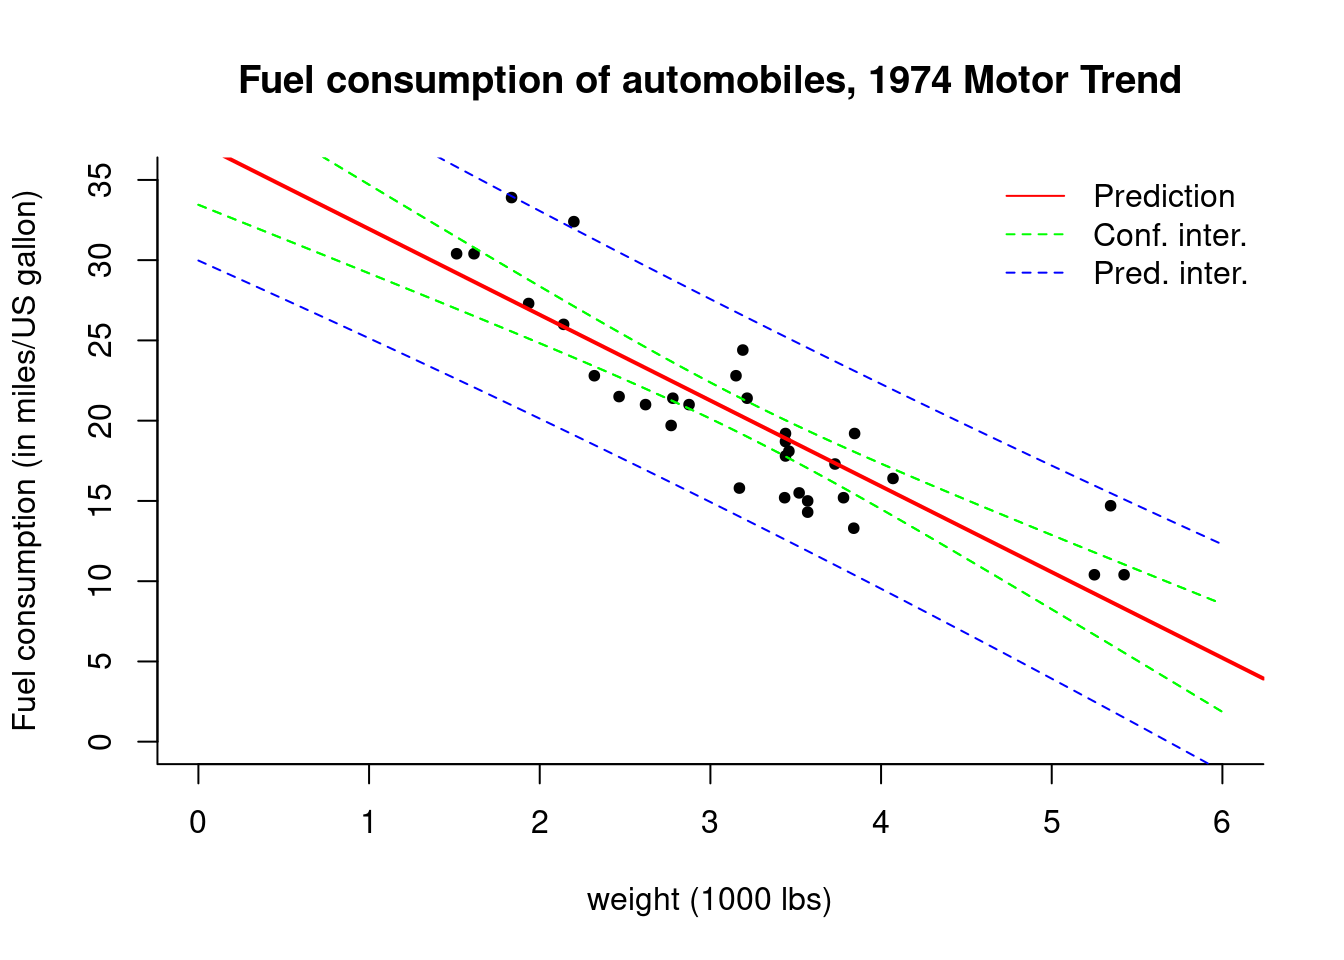
\includegraphics[width=0.7\linewidth]{LineaRModels_files/figure-latex/mtcars_confint-1} \end{center}

The function \texttt{predict} takes as imput a \texttt{data.frame} object containing the same column names as those of the fitted \texttt{lm} object. The names can be obtained from \texttt{names(ols\$model){[}-1{]}}.

As usual, we can verify we get the same result if we computed the intervals manually.

\begin{Shaded}
\begin{Highlighting}[]
\CommentTok{#Manually (see class notes)}
\NormalTok{confint_xstar <-}\StringTok{ }\NormalTok{tqu }\OperatorTok{*}\StringTok{ }\KeywordTok{sqrt}\NormalTok{(s2 }\OperatorTok{*}\StringTok{ }\KeywordTok{apply}\NormalTok{(}\KeywordTok{cbind}\NormalTok{(}\DecValTok{1}\NormalTok{, xstar), }\DecValTok{1}\NormalTok{, }\ControlFlowTok{function}\NormalTok{(cvec)\{}\KeywordTok{t}\NormalTok{(cvec) }\OperatorTok\StringTok{ }\KeywordTok{solve}\NormalTok{(}\KeywordTok{crossprod}\NormalTok{(X)) }\OperatorTok\StringTok{ }\NormalTok{cvec\}))}
\NormalTok{fitted_xstar <-}\StringTok{ }\KeywordTok{cbind}\NormalTok{(}\DecValTok{1}\NormalTok{, xstar) }\OperatorTok\StringTok{ }\KeywordTok{cbind}\NormalTok{(beta_hat)}
\KeywordTok{lines}\NormalTok{(xstar,  fitted_xstar }\OperatorTok{-}\StringTok{ }\NormalTok{confint_xstar, }\DataTypeTok{lty =} \DecValTok{2}\NormalTok{, }\DataTypeTok{col =} \StringTok{'green'}\NormalTok{)}
\KeywordTok{lines}\NormalTok{(xstar,  fitted_xstar }\OperatorTok{+}\StringTok{ }\NormalTok{confint_xstar, }\DataTypeTok{lty =} \DecValTok{2}\NormalTok{, }\DataTypeTok{col =} \StringTok{'green'}\NormalTok{)}
\end{Highlighting}
\end{Shaded}

\hypertarget{residuals}{%
\section{Residuals}\label{residuals}}

There are many types of residuals. The model residuals are simply \(\boldsymbol{e}=\mathbf{M}_{\mathbf{X}}\boldsymbol{y}\), which can be obtained through \texttt{resid} for \texttt{lm} objects.
We can verify numerically that \(\hat{{\boldsymbol{y}}} \perp \boldsymbol{e}\) and verify that \(\mathbf{X}^\top\boldsymbol{e}=\boldsymbol{0}_p\).

\begin{Shaded}
\begin{Highlighting}[]
\CommentTok{#Fitted values    }
\NormalTok{yhat <-}\StringTok{ }\KeywordTok{fitted}\NormalTok{(ols)}
\CommentTok{#Residuals}
\NormalTok{e <-}\StringTok{ }\KeywordTok{resid}\NormalTok{(ols)}

\CommentTok{#Orthogonality (by construction)}
\KeywordTok{isTRUE}\NormalTok{(}\KeywordTok{all.equal}\NormalTok{(}\KeywordTok{c}\NormalTok{(e }\OperatorTok\StringTok{ }\NormalTok{yhat), }\DecValTok{0}\NormalTok{))}
\end{Highlighting}
\end{Shaded}

\begin{verbatim}
## [1] TRUE
\end{verbatim}

\begin{Shaded}
\begin{Highlighting}[]
\KeywordTok{isTRUE}\NormalTok{(}\KeywordTok{all.equal}\NormalTok{(}\KeywordTok{c}\NormalTok{(e }\OperatorTok\StringTok{ }\NormalTok{X), }\KeywordTok{rep}\NormalTok{(}\DecValTok{0}\NormalTok{, }\DecValTok{2}\NormalTok{)))}
\end{Highlighting}
\end{Shaded}

\begin{verbatim}
## [1] TRUE
\end{verbatim}

In the sequel, we will look at calculation of various variants of the residuals. The first are the standardized residuals, also internally studentized residuals. These are defined as \(r_i = e_i/\{s(1-h_{ii})^{1/2}\}\), i.e.~each residual \(e_i\) is scaled by its individual variance to create homoscedastic residuals \(r_i\).

\begin{Shaded}
\begin{Highlighting}[]
\CommentTok{#we divide so they have the same variance - but not independent}
\NormalTok{r <-}\StringTok{ }\NormalTok{e}\OperatorTok{/}\KeywordTok{sqrt}\NormalTok{(s2}\OperatorTok{*}\NormalTok{(}\DecValTok{1}\OperatorTok{-}\NormalTok{leverage)) }
\CommentTok{#also obtainable via rstandard(ols)}
\KeywordTok{isTRUE}\NormalTok{(}\KeywordTok{all.equal}\NormalTok{(}\KeywordTok{rstandard}\NormalTok{(ols), r))}
\end{Highlighting}
\end{Shaded}

\begin{verbatim}
## [1] TRUE
\end{verbatim}

Because the \(i\)th residual is used in both the numerator and in the denominator (in the calculation of \(s^2\)), the standardized (internally studentized) residual follows marginally an approximate scaled Student distribution. However, because of the use of \(s^2\) in the denominator, the entries of \(\boldsymbol{r}\) are bounded by \(\pm n-p\). They are also not independent, even if this fact is often omitted in practice. While they will be approximately centered (with mean zero and variance one), they can (and should) be recentered before undertaking visual diagnostics.

The externally studentized residuals \(t_i\) are obtained by excluding the \(i\)th observation from the calculation of the variance. The advantage of doing this is that \(\{t_i\}_{i=1}^n\) are marginally Student distributed with \(n-p-1\) degrees of freedom (but they are again not independent). These are typically the residuals that are displayed in Q-Q plots. The externally studentized residuals can be obtained with the function \texttt{rstudent}.

We will derive formulas for \(\hat{\boldsymbol{\beta}}_{-i}\), \(s^2_{-i}\), Cook distance and \(t_i\) later in the exercises. Two of these are used below, namely
\[t_i =  \frac{e_i}{[s^2_{-i}(1-h_{ii})]^{1/2}}, \qquad s^2_{-i} = \frac{(n-p)s^2 -e_i^2/(1-h_{ii})}{n-p-1}. \]

\begin{Shaded}
\begin{Highlighting}[]
\CommentTok{#Externally studentized residuals}
\NormalTok{smi <-}\StringTok{ }\KeywordTok{influence}\NormalTok{(ols)}\OperatorTok{$}\NormalTok{sigma}
\NormalTok{s2mi <-((n}\DecValTok{-2}\NormalTok{)}\OperatorTok{*}\NormalTok{s2}\OperatorTok{-}\NormalTok{e}\OperatorTok{^}\DecValTok{2}\OperatorTok{/}\NormalTok{(}\DecValTok{1}\OperatorTok{-}\NormalTok{leverage))}\OperatorTok{/}\NormalTok{(n}\DecValTok{-3}\NormalTok{)}
\KeywordTok{isTRUE}\NormalTok{(}\KeywordTok{all.equal}\NormalTok{(smi}\OperatorTok{^}\DecValTok{2}\NormalTok{, s2mi))}
\end{Highlighting}
\end{Shaded}

\begin{verbatim}
## [1] TRUE
\end{verbatim}

\begin{Shaded}
\begin{Highlighting}[]
\NormalTok{esr <-}\StringTok{ }\NormalTok{e}\OperatorTok{/}\KeywordTok{sqrt}\NormalTok{(s2mi}\OperatorTok{*}\NormalTok{(}\DecValTok{1}\OperatorTok{-}\NormalTok{leverage))}
\KeywordTok{isTRUE}\NormalTok{(}\KeywordTok{all.equal}\NormalTok{(}\KeywordTok{rstudent}\NormalTok{(ols), esr))}
\end{Highlighting}
\end{Shaded}

\begin{verbatim}
## [1] TRUE
\end{verbatim}

The last type of residual is the leave-one-out cross validation residual. These are the residuals obtained by fitting the linear model to all observations, but the \(i\)th, i.e.,
\(\boldsymbol{y}_{-i}= \mathbf{X}_{-i}\boldsymbol{\beta}+ \boldsymbol{\varepsilon}\). Let \(\hat{\boldsymbol{\beta}}_{-i}\) denote the OLS coefficients from this regression and \(\hat{y}_{i,-i}=\mathbf{x}_i\hat{\boldsymbol{\beta}}_{-i}\) the predicted value for the left-out \(\mathbf{x}_i\) regressor. The \(i\)th leave-one-out cross validation residual is \(e_{i,-i}=y_i - \hat{y}_{i,-i}=e_i/(1-h_{ii})\). We can use these to calculate the PRESS statistic, \(\mathsf{PRESS}=\sum_{i=1}^n e_{i, -i}^2\)

\begin{Shaded}
\begin{Highlighting}[]
\CommentTok{# LOOCV residuals e/(1-leverage)}
\NormalTok{loocv <-}\StringTok{ }\NormalTok{e}\OperatorTok{/}\NormalTok{(}\DecValTok{1}\OperatorTok{-}\NormalTok{leverage)}
\NormalTok{loocv_err <-}\StringTok{ }\KeywordTok{rstandard}\NormalTok{(ols, }\DataTypeTok{type =} \StringTok{"pred"}\NormalTok{)}
\NormalTok{PRESS <-}\StringTok{ }\KeywordTok{crossprod}\NormalTok{(loocv_err)}
\end{Highlighting}
\end{Shaded}

\hypertarget{diagnostic-plots}{%
\section{Diagnostic plots}\label{diagnostic-plots}}

If the underlying model is truly linear, a plot of \(\boldsymbol{e}\) against \(\hat{\boldsymbol{y}}\), should be flat because the two are by construction orthogonal. In practice, we rescale \(\boldsymbol{e}\) by \(s\) to ensure that the variance is closer to unity. If there are omitted higher-order interactions, these will show up in such a plot.

In practice, there is often little difference between the rescaled residuals \(\boldsymbol{e}/s\) and the internally studentized residuals \(\boldsymbol{r}\). The former are orthogonal to \(\hat{\boldsymbol{y}}\), while the latter have equal variance.

\begin{Shaded}
\begin{Highlighting}[]
\KeywordTok{par}\NormalTok{(}\DataTypeTok{mfrow =} \KeywordTok{c}\NormalTok{(}\DecValTok{1}\NormalTok{, }\DecValTok{2}\NormalTok{)) }\CommentTok{#split the graphic window (1 row, 2 columns)}
\CommentTok{#Fitted values vs raw residuals/s2}
\KeywordTok{plot}\NormalTok{(}\DataTypeTok{y =}\NormalTok{ e}\OperatorTok{/}\KeywordTok{sqrt}\NormalTok{(s2), }\DataTypeTok{x =}\NormalTok{ yhat, }
     \DataTypeTok{xlab =} \StringTok{"fitted values"}\NormalTok{, }\DataTypeTok{ylab =} \StringTok{"rescaled residuals"}\NormalTok{); }\KeywordTok{abline}\NormalTok{(}\DataTypeTok{h =} \DecValTok{0}\NormalTok{, }\DataTypeTok{lty =} \DecValTok{2}\NormalTok{)}
\CommentTok{#Fitted values vs internally studentized residuals}
\KeywordTok{points}\NormalTok{(}\DataTypeTok{y =}\NormalTok{ r, }\DataTypeTok{x =}\NormalTok{ yhat, }\DataTypeTok{pch =} \DecValTok{20}\NormalTok{, }\DataTypeTok{col =} \DecValTok{2}\NormalTok{)}
\CommentTok{#Regressor weight vs residuals}
\KeywordTok{plot}\NormalTok{(}\DataTypeTok{y =}\NormalTok{ e}\OperatorTok{/}\KeywordTok{sqrt}\NormalTok{(s2), }\DataTypeTok{x =}\NormalTok{ X[,}\DecValTok{2}\NormalTok{], }\DataTypeTok{xlab =} \StringTok{"weight"}\NormalTok{, }
     \DataTypeTok{ylab =} \StringTok{"rescaled residuals"}\NormalTok{); }\KeywordTok{abline}\NormalTok{(}\DataTypeTok{h =} \DecValTok{0}\NormalTok{, }\DataTypeTok{lty =} \DecValTok{2}\NormalTok{)}
\KeywordTok{points}\NormalTok{(}\DataTypeTok{y =}\NormalTok{ r, }\DataTypeTok{x =}\NormalTok{ mtcars}\OperatorTok{$}\NormalTok{wt, }\DataTypeTok{pch =} \DecValTok{20}\NormalTok{, }\DataTypeTok{col =} \DecValTok{2}\NormalTok{)}
\end{Highlighting}
\end{Shaded}

\begin{center}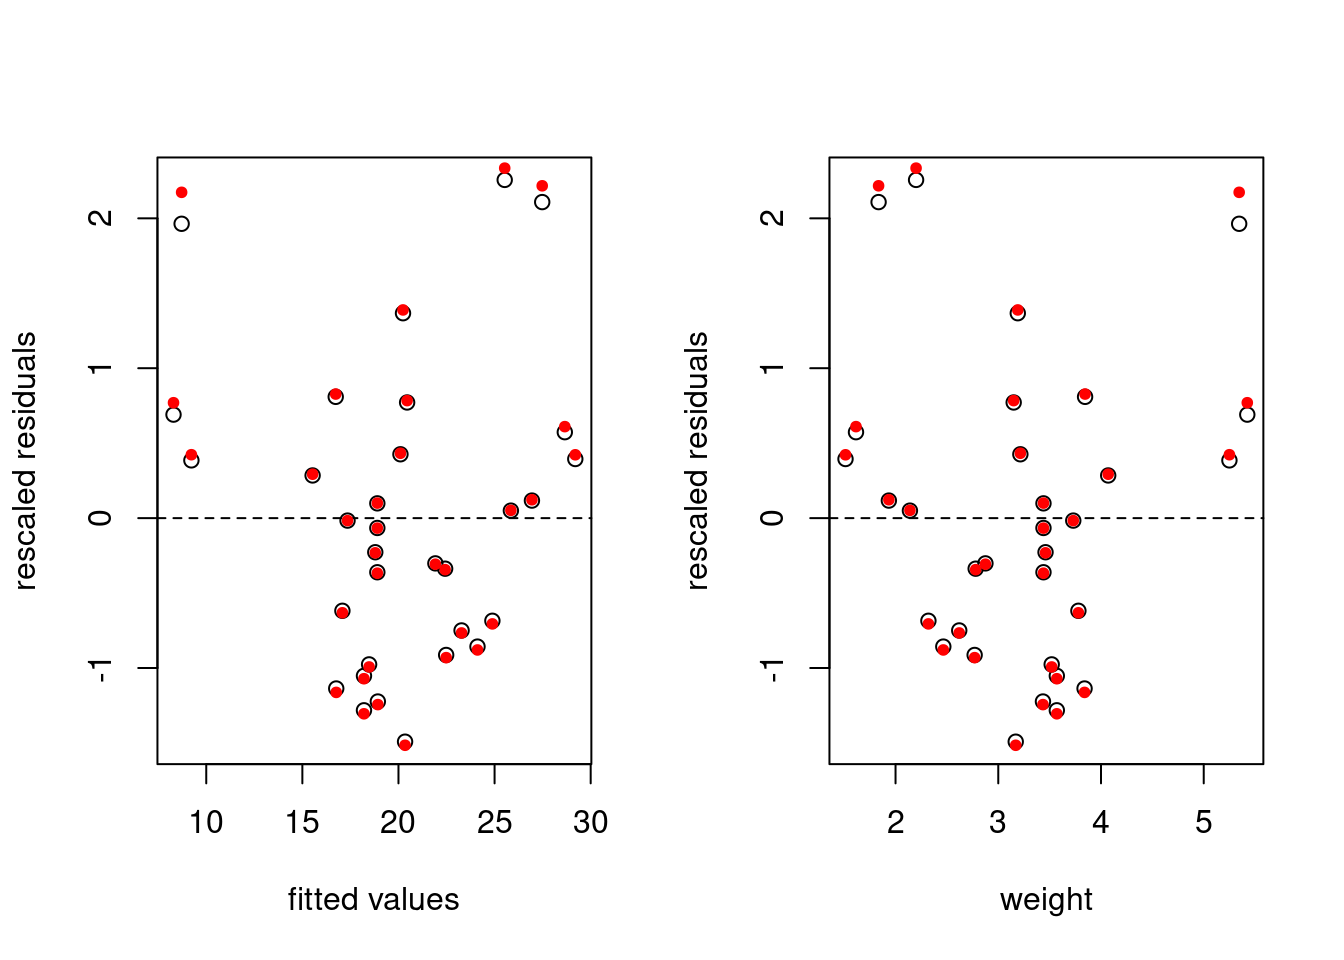
\includegraphics[width=0.7\linewidth]{LineaRModels_files/figure-latex/diagnostics-1} \end{center}

\begin{Shaded}
\begin{Highlighting}[]
\CommentTok{#graphics.off()}
\KeywordTok{par}\NormalTok{(}\DataTypeTok{mfrow =} \KeywordTok{c}\NormalTok{(}\DecValTok{1}\NormalTok{, }\DecValTok{1}\NormalTok{))}
\end{Highlighting}
\end{Shaded}

An alternative is \texttt{residualPlot(lm(mpg\ \textasciitilde{}\ hp\ +\ wt,\ data\ =\ mtcars))}, which adds the line for a quadratic regression of \(\hat{\boldsymbol{y}}\) against standardized residuals.

\hypertarget{added-variable-plots}{%
\subsection{Added-variable plots}\label{added-variable-plots}}

We can assess graphically whether a regressor should be included or not in the model. If the omitted regressor \(\mathbf{X}_2\) is redundant, its coefficient should be zero and we can project onto the orthogonal complement of the remaining regressors \(\mathbf{M}_{\mathbf{X}_1}\) and the response to get the regression FWL for \(\boldsymbol{\beta}_2\). The relationship between the two should have zero slope.
The package \texttt{car} has a function \texttt{avPlot}.

In the regression of fuel consumption as a function of weight, we have not included the potentially important regressor \texttt{hp}, which measures the power of the engine. The added variable plot shows that it is an important explanatory variable. In contrast, the displacement \texttt{disp} is either uncorrelated with \texttt{mpg} or its effect is already explained by \texttt{wt} and \texttt{hp}.

\begin{Shaded}
\begin{Highlighting}[]
\CommentTok{#install.packages("car")}
\KeywordTok{library}\NormalTok{(car)}
\NormalTok{car}\OperatorTok{::}\KeywordTok{avPlots}\NormalTok{(}\DataTypeTok{model =} \KeywordTok{lm}\NormalTok{(mpg }\OperatorTok{~}\StringTok{ }\NormalTok{hp }\OperatorTok{+}\StringTok{ }\NormalTok{wt }\OperatorTok{+}\StringTok{ }\NormalTok{disp, }\DataTypeTok{data =}\NormalTok{ mtcars))}
\end{Highlighting}
\end{Shaded}

\begin{center}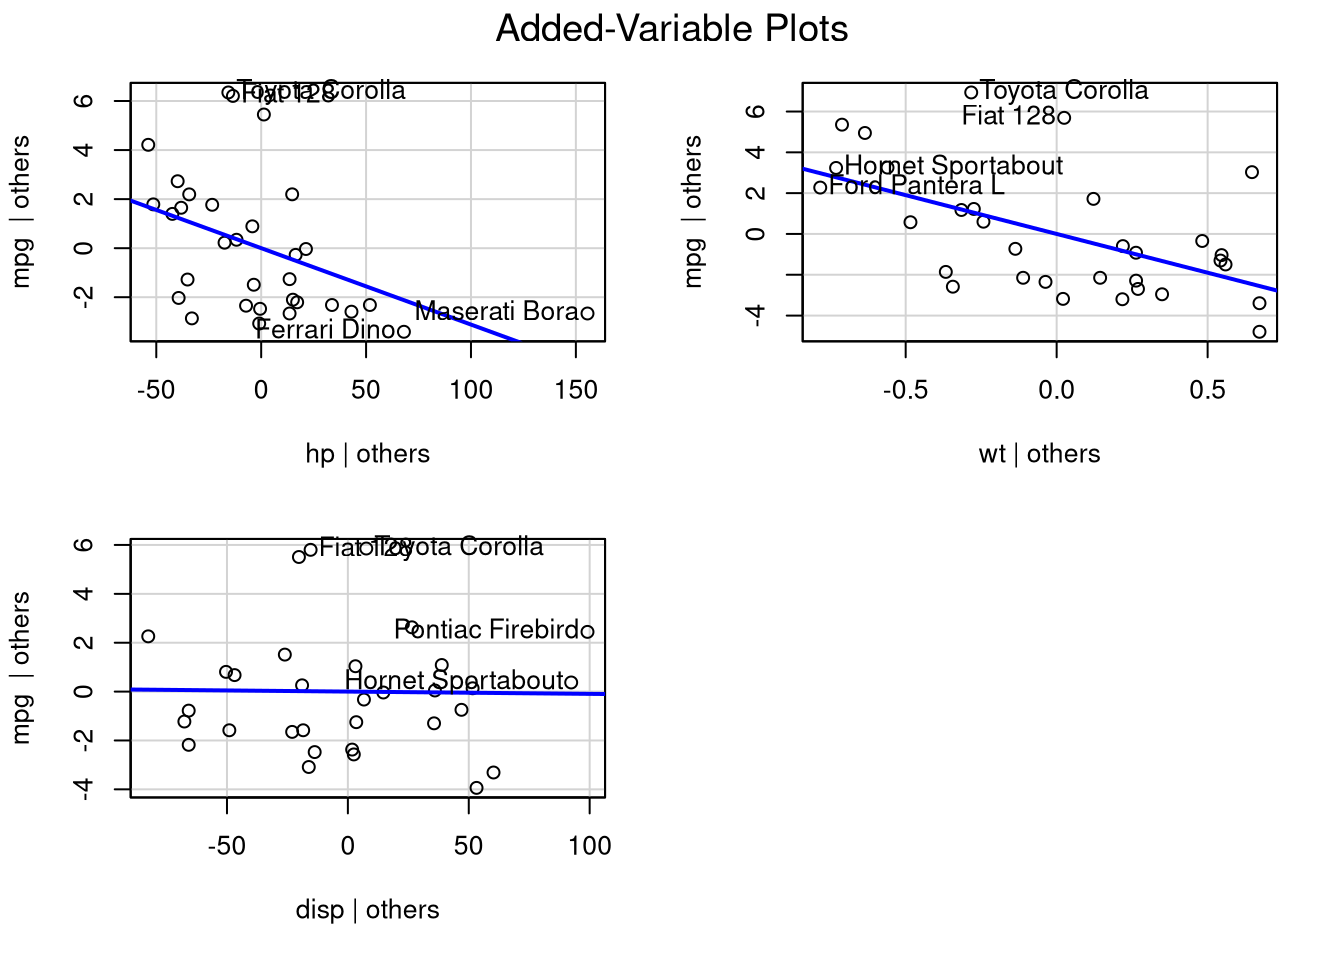
\includegraphics[width=0.7\linewidth]{LineaRModels_files/figure-latex/unnamed-chunk-23-1} \end{center}

\hypertarget{diagnostic-of-heteroscedasticity}{%
\subsection{Diagnostic of heteroscedasticity}\label{diagnostic-of-heteroscedasticity}}

Unequal variance will often show up in time series. For example, many economic models postulate exponential growth, but this effect can appear linear at a small scale. However, the variance will not be constant and typically increase with the level of the observations.
If there are factors, these may have different variances. A simple boxplot of the fitted values against the factor can flag heteroscedasticity.

\hypertarget{outliers}{%
\subsection{Outliers}\label{outliers}}

If an outlier is present and it has high leverage, it will draw the regression line towards itself. One way of assessing this (assuming there is a single such point) is to compute \(\hat{\boldsymbol{\beta}}\) by fitting the model to all but the observation \(y_i\). The difference between this estimate \(\hat{\boldsymbol{\beta}}_{-i}\) and \(\hat{\boldsymbol{\beta}}\) is called difference of betas, or \texttt{dfbeta}. We can compute the effect of the deletion efficiently (details later on this) and similarly rescale the estimates to get a standardized difference.

We can also look at the Cook's distance, the leverage values and the externally studentized residuals. These are often combined in a bubble pplot in which the radius of the circle is proportional to Cook's distance, with the leverage on the \(x\)-axis and the value of the externally studentized residuals \(\boldsymbol{t}\) on the \(y\)-axis.

\begin{Shaded}
\begin{Highlighting}[]
\KeywordTok{dfbetaPlots}\NormalTok{(}\DataTypeTok{model =} \KeywordTok{lm}\NormalTok{(mpg }\OperatorTok{~}\StringTok{ }\NormalTok{hp }\OperatorTok{+}\StringTok{ }\NormalTok{wt, }\DataTypeTok{data =}\NormalTok{ mtcars))}
\end{Highlighting}
\end{Shaded}

\begin{center}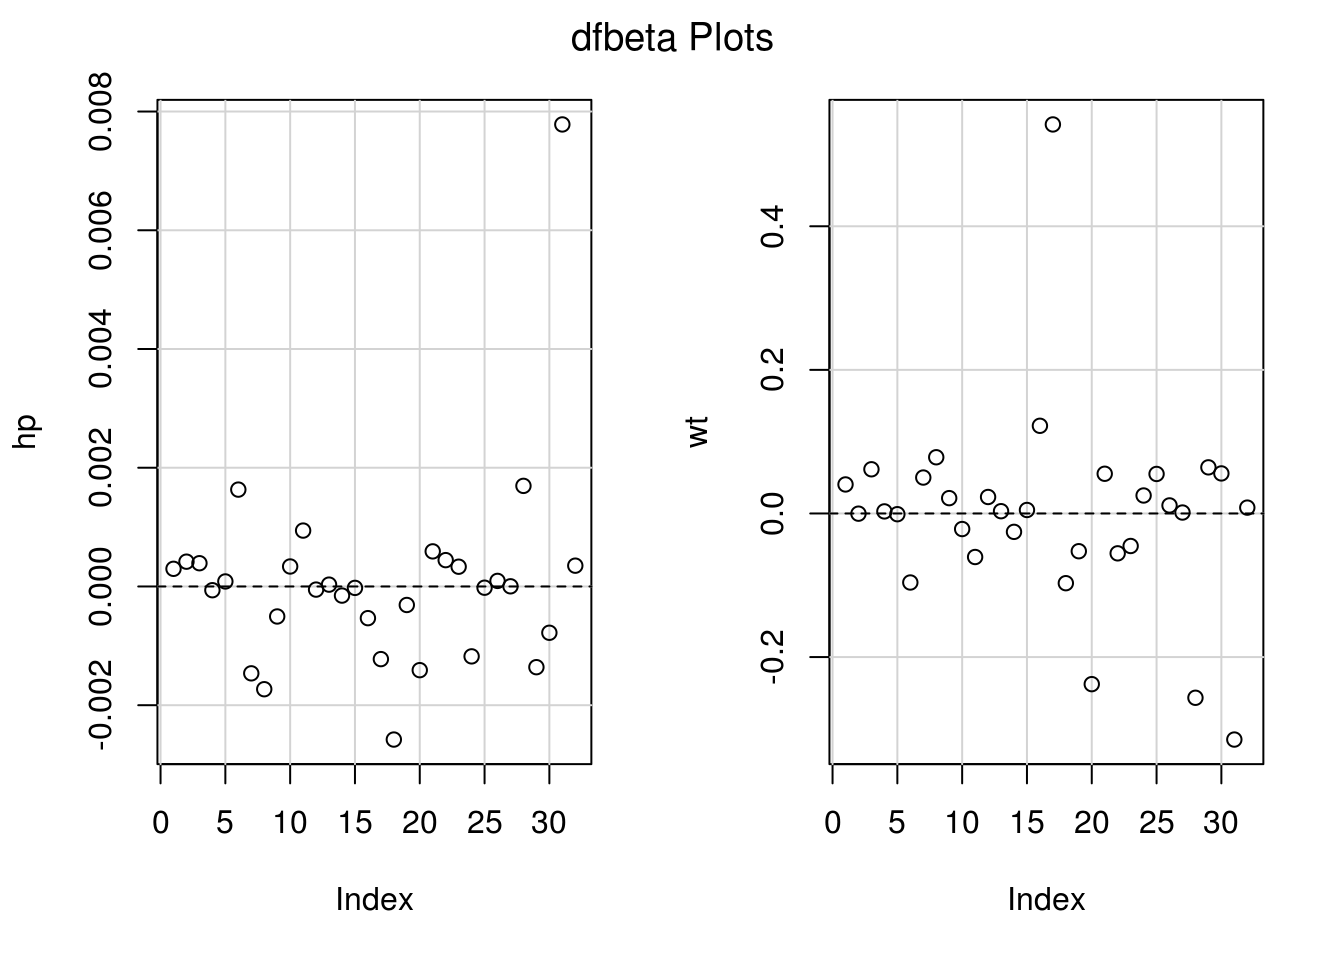
\includegraphics[width=0.7\linewidth]{LineaRModels_files/figure-latex/dfbeta-1} \end{center}

\begin{Shaded}
\begin{Highlighting}[]
\KeywordTok{influencePlot}\NormalTok{(}\DataTypeTok{model =} \KeywordTok{lm}\NormalTok{(mpg }\OperatorTok{~}\StringTok{ }\NormalTok{hp }\OperatorTok{+}\StringTok{ }\NormalTok{wt, }\DataTypeTok{data =}\NormalTok{ mtcars))}
\end{Highlighting}
\end{Shaded}

\begin{center}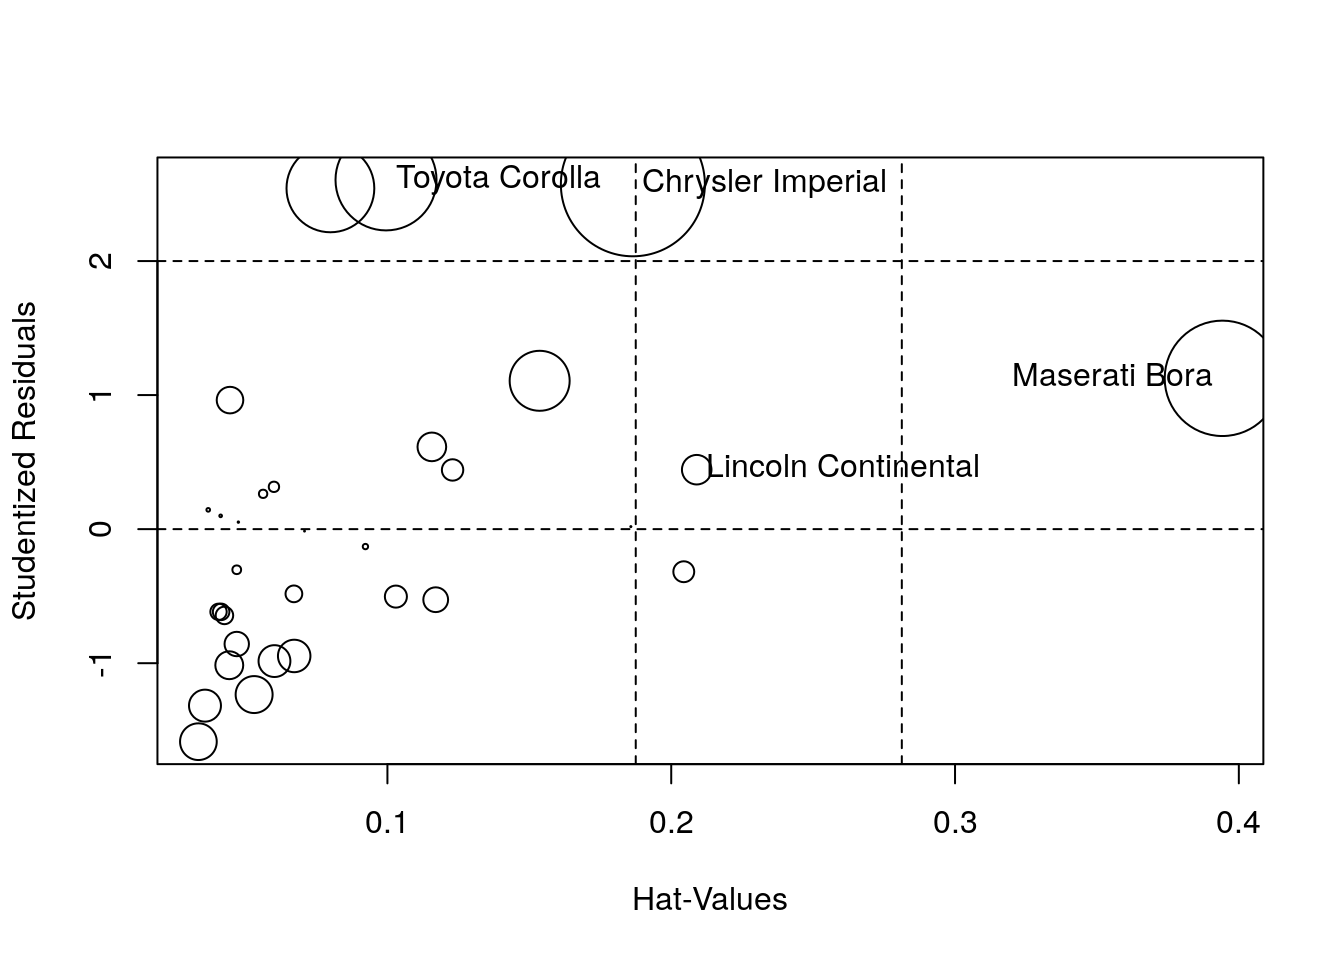
\includegraphics[width=0.7\linewidth]{LineaRModels_files/figure-latex/dfbeta-2} \end{center}

\begin{verbatim}
##                       StudRes        Hat     CookD
## Lincoln Continental 0.4434296 0.20897838 0.0178091
## Chrysler Imperial   2.5724776 0.18648721 0.4236109
## Toyota Corolla      2.6051516 0.09950335 0.2083933
## Maserati Bora       1.1250084 0.39420816 0.2720397
\end{verbatim}

\hypertarget{qqplot}{%
\section{Quantile-quantile plots}\label{qqplot}}

The distributional assumption is mostly assessed using quantile-quantile plots. However, the latter are hardly useful unless we superimpose some confidence intervals to the graph.
We will cover two methods for producing Q-Q plots for linear models: one using an orthogonal transformation that makes the estimated residuals IID. The second uses the externally studentized residuals.

\hypertarget{quantile-quantile-plot-of-externally-studentized-errors}{%
\subsection{Quantile-quantile plot of externally studentized errors}\label{quantile-quantile-plot-of-externally-studentized-errors}}

Recall that the quantile-quantile plot has

\begin{itemize}
\tightlist
\item
  on the \(x\)-axis, the theoretical quantiles, \(F^{-1}(\mathrm{rank}(X_i)/(n+1))\)
\item
  on the \(y\)-axis, the empirical quantiles, \(X_i\)
\end{itemize}

For a Gaussian Q-Q plot, we will need to estimate both the mean and the variance. The usual estimators will do, replacing \(\sigma^2\) with \(s^2\) in the calculations, but all results will be approximate. One can obtain standard residuals by subtracting the mean and scaling by the standard deviation (using e.g.~the function \texttt{scale}). The function \texttt{qqnorm} plots a Normal Q-Q plot without rescaling and the function \texttt{qqline} adds a line passing through the first and third quartile. Since these are robust estimates, this is a sensible option but implies that the scales of the Q-Q plot are not the same on the \(x\)-axis than on the \(y\)-axis. It is preferable to use these estimates to rescale the data, so as to facilitate the inclusion of approximate confidence intervals.

We now compute pointwise confidence intervals using the
result on the distribution of the order statistic, which will be covered in Exercise 9.2 (in 2018).

Suppose \(\{X_i\}_{i=1}^n\) are independent random variables with absolutely continuous distribution function \(F\) and density \(f\).
Let \(X_{(k)}\) denote the \(k\)th order statistic: \(X_{(1)} \leq \cdots \leq X_{(n)}\); then \(F(X_{(k)})\) follows a Beta distribution with parameters \(k\) and \(n + 1 - k\). Let \(\mathfrak{b}_{\eta}\) denote the \(\eta\)-quantile of the \(\mathsf{Beta}(k, n+1-k)\) distribution. Then,
\[\Pr\left\{\mathfrak{b}_{\alpha/2} \leq  F(X_{(k)}) \leq \mathfrak{b}_{1-\alpha/2}\right\} = 1-\alpha\]

so an approximate confidence interval for \(X_{(k)}\) is \([F^{-1}(\mathfrak{b}_{\alpha/2}), F^{-1}(\mathfrak{b}_{1-\alpha/2})]\).

\begin{Shaded}
\begin{Highlighting}[]
\CommentTok{#Student plotting position F^(-1)(E[U_\{(i)\}])}
\NormalTok{emp_quant <-}\StringTok{ }\KeywordTok{qt}\NormalTok{(}\KeywordTok{rank}\NormalTok{(esr)}\OperatorTok{/}\NormalTok{(n }\OperatorTok{+}\StringTok{ }\DecValTok{1}\NormalTok{),  }\DataTypeTok{df =}\NormalTok{ n }\OperatorTok{-}\StringTok{ }\DecValTok{3}\NormalTok{)  }
\CommentTok{#Function to compute the pointwise confidence intervals}
\CommentTok{#You can simply copy-paste this for your own plots}
\NormalTok{confint.qqplot.ptw <-}\StringTok{ }\ControlFlowTok{function}\NormalTok{(n, }\DataTypeTok{dist =} \StringTok{"norm"}\NormalTok{, ...)\{}
  \KeywordTok{t}\NormalTok{(}\KeywordTok{sapply}\NormalTok{(}\DecValTok{1}\OperatorTok{:}\NormalTok{n, }\ControlFlowTok{function}\NormalTok{(i)\{}
  \CommentTok{#Beta order statistic quantiles, mapped to Student scale}
    \KeywordTok{do.call}\NormalTok{(}\KeywordTok{paste0}\NormalTok{(}\StringTok{'q'}\NormalTok{, dist), }\KeywordTok{list}\NormalTok{(}\KeywordTok{qbeta}\NormalTok{(}\KeywordTok{c}\NormalTok{(}\FloatTok{0.025}\NormalTok{, }\FloatTok{0.975}\NormalTok{), i, n }\OperatorTok{-}\StringTok{ }\NormalTok{i }\OperatorTok{+}\StringTok{ }\DecValTok{1}\NormalTok{), ...))}
\NormalTok{  \}))}
\NormalTok{\}}

\CommentTok{#Call the function}
\NormalTok{confint_lim <-}\StringTok{ }\KeywordTok{confint.qqplot.ptw}\NormalTok{(}\DataTypeTok{n =}\NormalTok{ n, }\DataTypeTok{dist =} \StringTok{"t"}\NormalTok{, }\DataTypeTok{df =}\NormalTok{ n }\OperatorTok{-}\StringTok{ }\DecValTok{3}\NormalTok{)}
\CommentTok{#Plot these confidence bands alongside with the empirical quantile plotting position}
\KeywordTok{matplot}\NormalTok{(}\KeywordTok{sort}\NormalTok{(emp_quant), confint_lim, }\DataTypeTok{type =} \StringTok{"l"}\NormalTok{, }\DataTypeTok{lty =} \DecValTok{2}\NormalTok{, }\DataTypeTok{col=}\StringTok{"grey"}\NormalTok{,}
        \DataTypeTok{main =} \StringTok{"Normal Q-Q plot"}\NormalTok{, }\DataTypeTok{xlim =} \KeywordTok{c}\NormalTok{(}\OperatorTok{-}\DecValTok{2}\NormalTok{, }\DecValTok{2}\NormalTok{), }\DataTypeTok{ylim =} \KeywordTok{c}\NormalTok{(}\OperatorTok{-}\DecValTok{2}\NormalTok{, }\DecValTok{2}\NormalTok{),}
        \DataTypeTok{xlab =} \StringTok{"Theoretical quantiles"}\NormalTok{, }\DataTypeTok{ylab =} \StringTok{"Empirical quantiles"}\NormalTok{)  }
\CommentTok{#Theoretical line of fit}
\KeywordTok{abline}\NormalTok{(}\DataTypeTok{a =} \DecValTok{0}\NormalTok{, }\DataTypeTok{b =} \DecValTok{1}\NormalTok{)}
\CommentTok{#Add observations}
\KeywordTok{points}\NormalTok{(esr, emp_quant, }\DataTypeTok{pch =} \DecValTok{20}\NormalTok{)}
\end{Highlighting}
\end{Shaded}

\begin{center}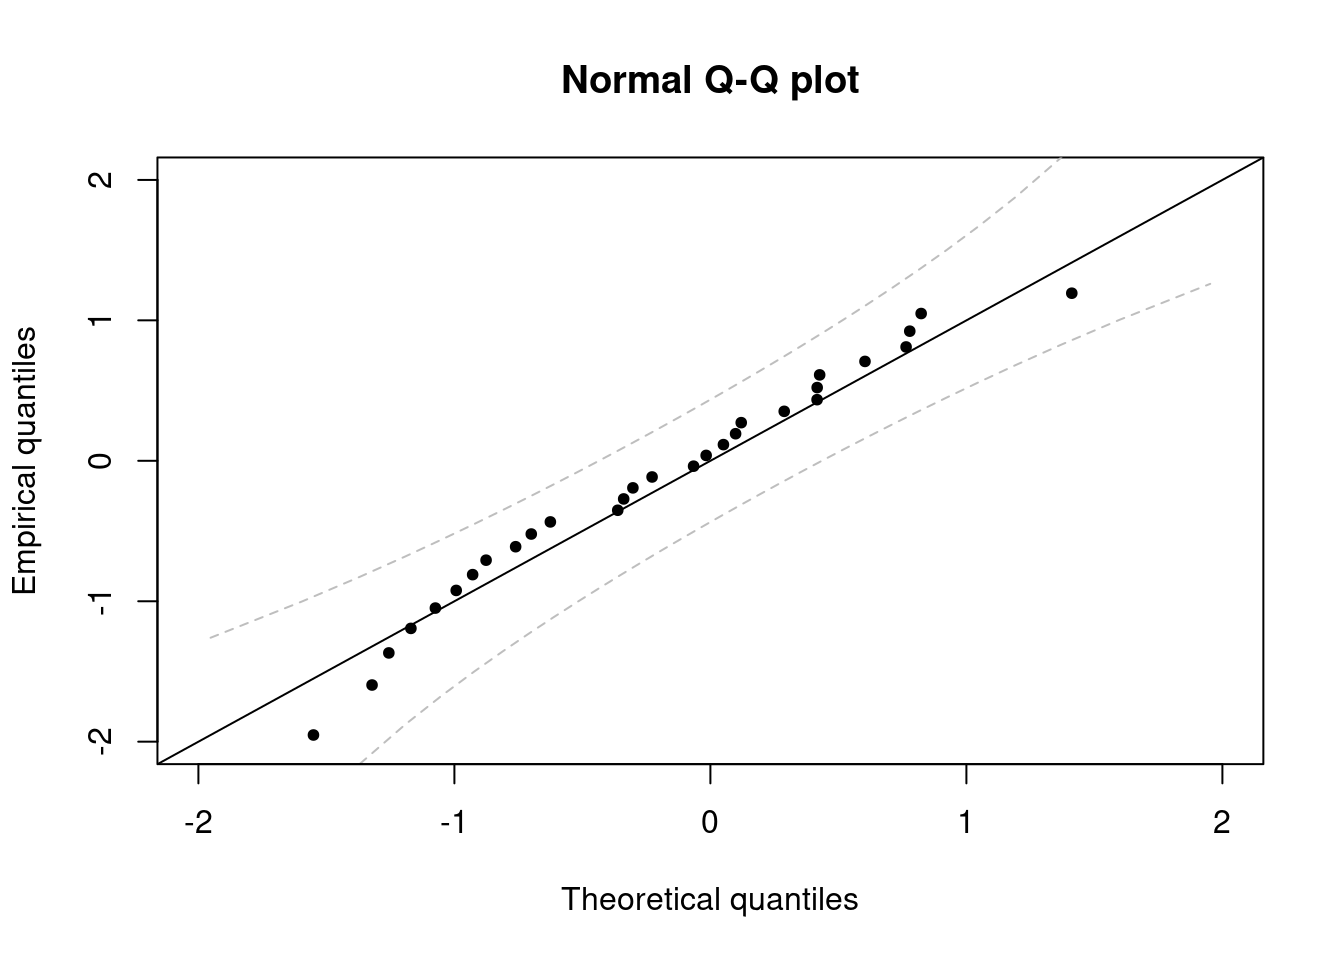
\includegraphics[width=0.7\linewidth]{LineaRModels_files/figure-latex/unnamed-chunk-24-1} \end{center}

\hypertarget{quantile-quantile-plot-using-the-qr-decomposition}{%
\subsection{Quantile-quantile plot using the QR decomposition}\label{quantile-quantile-plot-using-the-qr-decomposition}}

The problem with the residuals is that, while \(\boldsymbol{e}\) are normally distributed with variance \(\sigma^2\mathbf{M}_{\mathbf{X}}\), they are linearly dependent (think of the constraint \(\mathbf{X}^\top\boldsymbol{e}=\boldsymbol{0}_p\)).

Therefore, \(\mathbf{M}_{\mathbf{X}}\) is not invertible (it is an \(n \times n\) matrix of rank \(n - p\)) --- \texttt{solve(diag(n)\ -\ Hmat)} typically returns an error message although some matrix decomposition such as the SVD handle the rank deficient case. One can use an orthogonal transformation to obtain a set of \(n-p\) independent residuals, but it is then difficult to relate these to the regressors.

One such orthogonal transformation is provided by the QR decomposition, \(\mathbf{X}=\mathbf{Q}\mathbf{R}\) where \(\mathbf{Q}\) is an orthogonal matrix. Consider the linear model \[\mathbf{Q}^\top\boldsymbol{Y} = \mathbf{Q}^\top\mathbf{X}\boldsymbol{\beta}+ \boldsymbol{u};\] the last \(n-p\) estimated residuals of the vector \(\tilde{\boldsymbol{e}} =\mathbf{Q}^\top\boldsymbol{e}\) will be IID Normal and the first \(p\) identically zero. In \texttt{R}, use the function \texttt{t(qr.Q(qr(X),\ complete\ =\ TRUE))} to obtain the matrix \(\mathbf{Q}^\top\) associated to the design matrix \texttt{X}.

Note that it is difficult to detect violation of the normality assumption because observations that arise from distributions that are not heavy-tailed still behave roughly like they are normally distributed when we scale them. This phenomenon, \emph{supernormality}, is a consequence of the central limit theorem.

\hypertarget{monte-carlo-methods-for-confidence-intervals}{%
\subsection{Monte Carlo methods for confidence intervals}\label{monte-carlo-methods-for-confidence-intervals}}

This section contains \textbf{optional} material. It contains advanced material that can be skipped upon first reading.

An alternative to asymptotic theory (which may be unreliable in small samples) is to rely on simulations. The idea is to obtain a statistic whose distribution is (at least asymptotically) pivotal, i.e.~fully specified under the null hypothesis. One can simulate samples from the null distribution \(B\) times and compare the resulting data points with the test statistic calculated from the observed sample. This method, which is termed bootstrap test, is particularly powerful when we want to obtain critical values for test statistics, like e.g.~\(\max(|t_i|)\), whose distribution is untractable.

Under the null hypothesis of the Gaussian linear model, \(\{y_i\}_{i=1}^n\) is a simple random sample from a Gaussian distribution \(\boldsymbol{Y} \sim \mathcal{N}_n(\mathbf{X}\boldsymbol{\beta}, \sigma^2 \mathbf{I}_n)\). One can resort to simulations to obtain approximate confidence intervals at asymptotic level \(\alpha\). Specifically, the postulated data generating mechanism is \[\boldsymbol{Y} = \mathbf{X}\boldsymbol{\beta} + \boldsymbol{\varepsilon}.\]
We will replace the unknown parameters (here \(\boldsymbol{\beta}\) and \(\sigma^2\)) by their best linear unbiased estimate. For \(b=1, \ldots, B\) where \(B/\alpha \in \mathbb{N}\), repeat the following steps:

\begin{enumerate}
\item sample $\boldsymbol{\varepsilon}_{b} \sim \mathcal{N}_n(\boldsymbol{0}_n, s^2\mathbf{I}_n)$ and form $\boldsymbol{y}_b = \mathbf{X} \hat{\boldsymbol{\beta}} + \boldsymbol{\varepsilon}_{b}$. 
\item run least squares with the design matrix $\mathbf{X}$ and extract the residuals $\boldsymbol{e}_b$. Compute 
the centered externally Studentized version.
\item sort the samples and the $\alpha/2$ and $1-\alpha/2$ empirical quantiles of each vector of order statistics
\end{enumerate}

This provides a pointwise confidence interval for each order statistic. We can assess the overall coverage of the intervals by checking whether or not one of the points falls outside the confidence envelope. Since we have \(B\) datasets, we can check each in turn (using the others as reference for the interval) and check the fraction that have at least one observations outside the simulated pointwise bands. This gives a measure of the overall error rate. We can adjust \(k\) until we get the correct overall empirical coverage.

The calculation is rather simple.

\begin{itemize}
\tightlist
\item
  calculate the rank of each observation (column by column) in the \(B \times n\) matrix of simulated points.
\item
  an exceedance occurs if and only if the rank of an observation in a line is below or equal to \(k\), or at least \(B+1-k\).
\item
  to check this, it suffices to retain the minimum and maximum rank of each row.
\end{itemize}

These methods are implemented in the package \texttt{boot} and returned by the function \texttt{boot::envelope}; you must supply a matrix of replicates test statistics. In our setting, these are the ordered samples from the externally studentized residuals \[\left\{\big\{t^{b}_{(i)}\big\}_{i=1}^n\right\}_{b=1}^B.\]

You should choose \(B\) so that \(B+1\) is divisible by \(\alpha\) and rather large. \(B = 9999\) should work well and not be too computationally costly for small datasets.

\begin{Shaded}
\begin{Highlighting}[]
\CommentTok{#Dimensions of the design matrix}
\NormalTok{n <-}\StringTok{ }\KeywordTok{nrow}\NormalTok{(}\KeywordTok{model.matrix}\NormalTok{(ols))}
\NormalTok{p <-}\StringTok{ }\KeywordTok{ncol}\NormalTok{(}\KeywordTok{model.matrix}\NormalTok{(ols))}
\CommentTok{#Bootstrap setting}
\NormalTok{B <-}\StringTok{ }\DecValTok{9999}
\NormalTok{X <-}\StringTok{ }\KeywordTok{model.matrix}\NormalTok{(ols)}
\NormalTok{betahat <-}\StringTok{ }\KeywordTok{coef}\NormalTok{(ols)}
\NormalTok{boot_samp <-}\StringTok{ }\KeywordTok{matrix}\NormalTok{(}\OtherTok{NA}\NormalTok{, }\DataTypeTok{nrow =}\NormalTok{ B, }\DataTypeTok{ncol =}\NormalTok{ n)}
\ControlFlowTok{for}\NormalTok{(b }\ControlFlowTok{in} \DecValTok{1}\OperatorTok{:}\NormalTok{B)\{}
  \CommentTok{#Generate new errors}
\NormalTok{  eps_samp <-}\StringTok{ }\KeywordTok{rnorm}\NormalTok{(n, }\DataTypeTok{sd =} \KeywordTok{sqrt}\NormalTok{(s2))}
\NormalTok{  Xbeta <-}\StringTok{ }\NormalTok{X }\OperatorTok\StringTok{ }\NormalTok{betahat}
  \CommentTok{#Create new replicate dataset}
\NormalTok{  yb <-}\StringTok{ }\NormalTok{Xbeta }\OperatorTok{+}\StringTok{ }\NormalTok{eps_samp}
  \CommentTok{#Obtain externally studentized residuals}
  \CommentTok{#Sort them in increasing order}
\NormalTok{  boot_samp[b, ] <-}\StringTok{ }\KeywordTok{sort}\NormalTok{(}\KeywordTok{rstudent}\NormalTok{(}\KeywordTok{lm}\NormalTok{(yb }\OperatorTok{~}\StringTok{ }\DecValTok{-1} \OperatorTok{+}\StringTok{ }\NormalTok{X)))}
\NormalTok{\}}

\CommentTok{#Add the dataset to the replicates}
\NormalTok{res_samp <-}\StringTok{ }\KeywordTok{rbind}\NormalTok{((esr <-}\StringTok{ }\KeywordTok{rstudent}\NormalTok{(ols)), boot_samp)}
\CommentTok{#Compute the quantiles of this experiment => per column means for each order statistic}
\NormalTok{confint_pw <-}\StringTok{ }\KeywordTok{t}\NormalTok{(}\KeywordTok{apply}\NormalTok{(res_samp, }\DecValTok{2}\NormalTok{, quantile, }\DataTypeTok{probs =} \KeywordTok{c}\NormalTok{(}\FloatTok{0.025}\NormalTok{, }\FloatTok{0.975}\NormalTok{)))}
\CommentTok{#Alternatively, could sort each column and pick the k and B-k-1 entries}

\CommentTok{#Computed automatically by package bootstrap}
\NormalTok{env <-}\StringTok{ }\NormalTok{boot}\OperatorTok{::}\KeywordTok{envelope}\NormalTok{(}\DataTypeTok{mat =}\NormalTok{ boot_samp)}

\CommentTok{#Plot the confidence interval}
\KeywordTok{matplot}\NormalTok{(}\DataTypeTok{y =} \KeywordTok{cbind}\NormalTok{(}\KeywordTok{sort}\NormalTok{(esr), confint_pw), }\DataTypeTok{x =} \KeywordTok{qt}\NormalTok{((}\DecValTok{1}\OperatorTok{:}\NormalTok{n) }\OperatorTok{/}\StringTok{ }\NormalTok{(n }\OperatorTok{+}\StringTok{ }\DecValTok{1}\NormalTok{), }\DataTypeTok{df =}\NormalTok{ n }\OperatorTok{-}\StringTok{ }\NormalTok{p }\OperatorTok{-}\StringTok{ }\DecValTok{1}\NormalTok{), }
       \DataTypeTok{lty =} \KeywordTok{c}\NormalTok{(}\DecValTok{1}\NormalTok{, }\DecValTok{2}\NormalTok{, }\DecValTok{2}\NormalTok{), }\DataTypeTok{col =} \KeywordTok{c}\NormalTok{(}\DecValTok{1}\NormalTok{, }\StringTok{"grey"}\NormalTok{, }\StringTok{"grey"}\NormalTok{), }\DataTypeTok{type =} \KeywordTok{c}\NormalTok{(}\StringTok{"p"}\NormalTok{,}\StringTok{"l"}\NormalTok{,}\StringTok{"l"}\NormalTok{), }
       \DataTypeTok{pch =} \DecValTok{20}\NormalTok{, }\DataTypeTok{xlab =} \StringTok{"Theoretical quantiles"}\NormalTok{, }\DataTypeTok{ylab =} \StringTok{"Empirical quantiles"}\NormalTok{, }\DataTypeTok{bty =} \StringTok{'l'}\NormalTok{)}
\KeywordTok{abline}\NormalTok{(}\DataTypeTok{a =} \DecValTok{0}\NormalTok{, }\DataTypeTok{b =} \DecValTok{1}\NormalTok{)}

\CommentTok{#Simultaneous confidence interval}
\CommentTok{#In how many of the replicates datasets do we have }
\CommentTok{#observations outside of the pointwise confidence bands?}
\NormalTok{R <-}\StringTok{ }\KeywordTok{nrow}\NormalTok{(boot_samp)}
\NormalTok{alpha <-}\StringTok{ }\FloatTok{0.05}
\NormalTok{k <-}\StringTok{ }\NormalTok{alpha }\OperatorTok{*}\StringTok{ }\NormalTok{(R }\OperatorTok{+}\StringTok{ }\DecValTok{1}\NormalTok{)}\OperatorTok{/}\DecValTok{2}
\CommentTok{#Simply check this as follows:}
\CommentTok{#For each column, return the rank of the simulation}
\NormalTok{rank_boot <-}\StringTok{ }\KeywordTok{apply}\NormalTok{(boot_samp, }\DecValTok{2}\NormalTok{, rank)}
\CommentTok{#For each row, keep minimum and maximum rank}
\NormalTok{minmax_rk <-}\StringTok{ }\KeywordTok{t}\NormalTok{(}\KeywordTok{apply}\NormalTok{(rank_boot, }\DecValTok{1}\NormalTok{, }\ControlFlowTok{function}\NormalTok{(x)\{}\KeywordTok{c}\NormalTok{(}\KeywordTok{min}\NormalTok{(x), }\KeywordTok{max}\NormalTok{(x))\}))}
\CommentTok{#Go outside of the pointwise confidence interval if }
\CommentTok{#min(rank) < k or max(rank) > R + 1 - k }
\NormalTok{emp_boot_cov <-}\StringTok{ }\ControlFlowTok{function}\NormalTok{(k)\{}
 \DecValTok{1}\OperatorTok{-}\KeywordTok{mean}\NormalTok{((}\KeywordTok{I}\NormalTok{(minmax_rk[,}\DecValTok{1}\NormalTok{] }\OperatorTok{>}\StringTok{ }\NormalTok{k))}\OperatorTok{*}\KeywordTok{I}\NormalTok{(minmax_rk[,}\DecValTok{2}\NormalTok{] }\OperatorTok{<}\StringTok{ }\NormalTok{(R}\OperatorTok{+}\DecValTok{1}\OperatorTok{-}\NormalTok{k)))}
\NormalTok{\}}
\CommentTok{#In how many of the replicates datasets do }
\CommentTok{#we have observations outside of the bounds?}
\KeywordTok{emp_boot_cov}\NormalTok{(k)}
\end{Highlighting}
\end{Shaded}

\begin{verbatim}
## [1] 0.5774577
\end{verbatim}

\begin{Shaded}
\begin{Highlighting}[]
\CommentTok{#Ouch! decrease k until we hit alpha percentage of exceedances (0.05)}
\NormalTok{boot_cov_k <-}\StringTok{ }\KeywordTok{sapply}\NormalTok{(}\DecValTok{1}\OperatorTok{:}\NormalTok{k, emp_boot_cov)}
\NormalTok{klev <-}\StringTok{ }\KeywordTok{match}\NormalTok{(}\OtherTok{TRUE}\NormalTok{, boot_cov_k }\OperatorTok{>}\StringTok{ }\NormalTok{alpha) }\OperatorTok{-}\StringTok{ }\DecValTok{1}
\ControlFlowTok{if}\NormalTok{(klev }\OperatorTok{==}\StringTok{ }\DecValTok{0}\NormalTok{)\{}
\NormalTok{ klev <-}\StringTok{ }\DecValTok{1}
\NormalTok{\}}
\NormalTok{env_jt <-}\StringTok{ }\KeywordTok{apply}\NormalTok{(boot_samp, }\DecValTok{2}\NormalTok{, sort)[}\KeywordTok{c}\NormalTok{(R}\OperatorTok{+}\DecValTok{1}\OperatorTok{-}\NormalTok{klev, klev),]}

\CommentTok{#This is what is returned by function envelope}
\KeywordTok{isTRUE}\NormalTok{(}\KeywordTok{all.equal}\NormalTok{(env_jt, env}\OperatorTok{$}\NormalTok{overall))}
\end{Highlighting}
\end{Shaded}

\begin{verbatim}
## [1] TRUE
\end{verbatim}

\begin{Shaded}
\begin{Highlighting}[]
\KeywordTok{matplot}\NormalTok{(}\DataTypeTok{x =} \KeywordTok{qt}\NormalTok{((}\DecValTok{1}\OperatorTok{:}\NormalTok{n)}\OperatorTok{/}\NormalTok{(n}\OperatorTok{+}\DecValTok{1}\NormalTok{), }\DataTypeTok{df =}\NormalTok{ n }\OperatorTok{-}\StringTok{ }\NormalTok{p }\DecValTok{-1}\NormalTok{), }\DataTypeTok{y =} \KeywordTok{t}\NormalTok{(env}\OperatorTok{$}\NormalTok{overall), }
       \DataTypeTok{col =} \StringTok{"darkgrey"}\NormalTok{, }\DataTypeTok{add =} \OtherTok{TRUE}\NormalTok{, }\DataTypeTok{type =} \StringTok{"l"}\NormalTok{, }\DataTypeTok{lty =} \DecValTok{1}\NormalTok{)}
\end{Highlighting}
\end{Shaded}

\begin{center}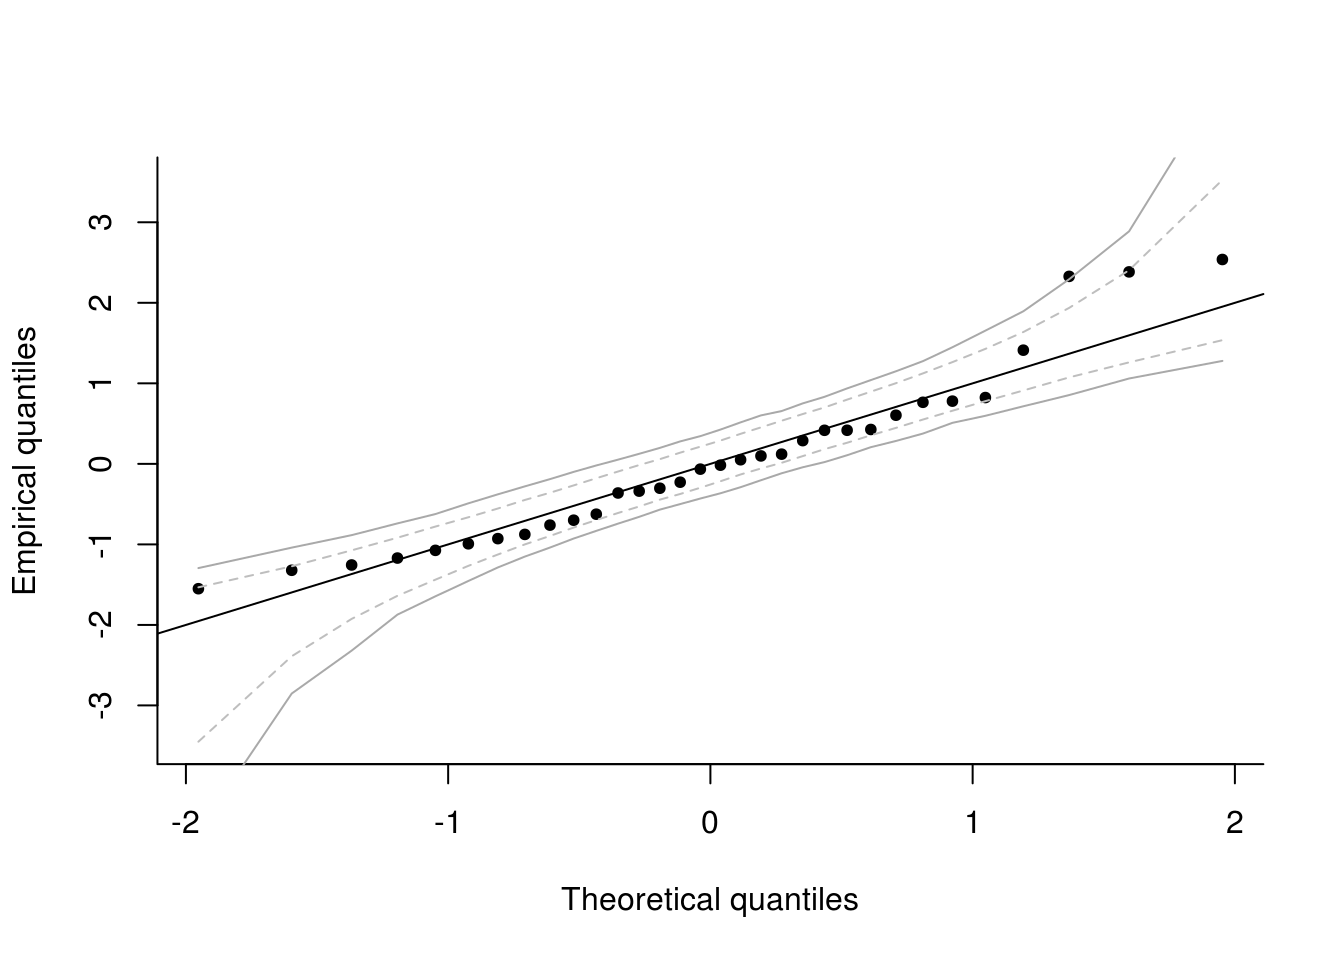
\includegraphics[width=0.7\linewidth]{LineaRModels_files/figure-latex/unnamed-chunk-25-1} \end{center}

\hypertarget{parametric-bootstrap-confidence-intervals-using-the-qr-decomposition}{%
\subsection{Parametric bootstrap confidence intervals using the QR decomposition}\label{parametric-bootstrap-confidence-intervals-using-the-qr-decomposition}}

This section contains \textbf{optional} material.

There is an alternative way to obtain pointwise (and even simultaneous) confidence intervals for the QR decomposition.
Under the null hypothesis: \(\boldsymbol{\varepsilon} \sim \mathcal{N}_{n}(\mathbf{0}_n, \sigma^2\mathbf{I}_n)\), we get \(\tilde{\boldsymbol{\varepsilon}} \sim \mathcal{N}_{n-p}(\mathbf{0}_n, \sigma^2\mathbf{I}_n)\) and therefore \((\tilde{\boldsymbol{\varepsilon}}- \overline{\boldsymbol{\tilde{\varepsilon}}})/\mathrm{sd}(\boldsymbol{\tilde{\varepsilon}}) \stackrel{\cdot}{\sim} \mathcal{N}_{n-p}(\mathbf{0}_n, \mathbf{I}_n)\) is asymptotically pivotal. A pivotal quantity has a fully specified distribution.

We have only observed one sample, so comparisons are difficult because the measurements are limited.
Under the null hypothesis, it is however easy to generate new datasets: simply generate new observations
\(\tilde{\boldsymbol{\epsilon}}_b \sim \mathcal{N}_{n-p}(\mathbf{0}_n, \mathbf{I}_n)\) and standardize them, mimicking what we have done to obtain our sample quantiles.
This gives us a potentially unlimited number of samples to compare our observations to.
By ordering each new set of errors of the \(B\) replicates, we get a matrix of observations whose rows are order statistics from a run and whose columns corresponds to the empirical distribution of each order statistic. A symmetric 95\% confidence interval is obtained by taking the empirical (0.025, 0.975) percentiles of each order statistic.

\hypertarget{solutions-3}{%
\section{Solutions}\label{solutions-3}}

\hypertarget{exercise-7.1---study-of-growth-hormones}{%
\subsection{Exercise 7.1 - Study of growth hormones}\label{exercise-7.1---study-of-growth-hormones}}

We will use \texttt{factor} objects in the sequel. A \texttt{factor} encodes a matrix of binary variables,
potentially identied using strings, so that the output is readable. \textbf{R} know how to handle the vector if it is passed to e.g.~the function \texttt{lm}. By default, if the matrix spans \(\mathbf{1}_n\), the first level (in alphabetical order) is dropped and the intercept becomes the mean of this level.

\begin{Shaded}
\begin{Highlighting}[]
\NormalTok{url1 <-}\StringTok{ "https://lbelzile.bitbucket.io/math341/growth.dat"}
\NormalTok{growth <-}\StringTok{ }\KeywordTok{read.table}\NormalTok{(url1, }\DataTypeTok{header =} \OtherTok{TRUE}\NormalTok{)}
\KeywordTok{summary}\NormalTok{(growth)}
\end{Highlighting}
\end{Shaded}

\begin{verbatim}
##        y               x             group          
##  Min.   :107.0   Min.   : 78.00   Length:20         
##  1st Qu.:122.0   1st Qu.: 93.75   Class :character  
##  Median :140.0   Median :100.50   Mode  :character  
##  Mean   :142.4   Mean   :100.90                     
##  3rd Qu.:156.5   3rd Qu.:109.25                     
##  Max.   :185.0   Max.   :123.00
\end{verbatim}

\begin{Shaded}
\begin{Highlighting}[]
\CommentTok{##Check what the factor encodes: transpose of design matrix}
\KeywordTok{t}\NormalTok{(}\KeywordTok{model.matrix}\NormalTok{(y }\OperatorTok{~}\StringTok{ }\NormalTok{group }\OperatorTok{-}\StringTok{ }\DecValTok{1}\NormalTok{, }\DataTypeTok{data=}\NormalTok{ growth))}
\end{Highlighting}
\end{Shaded}

\begin{verbatim}
##                 1 2 3 4 5 6 7 8 9 10 11 12 13 14 15 16 17 18 19 20
## groupcontrol    1 1 1 1 1 1 1 1 1  1  0  0  0  0  0  0  0  0  0  0
## groupthiouracil 0 0 0 0 0 0 0 0 0  0  1  1  1  1  1  1  1  1  1  1
## attr(,"assign")
## [1] 1 1
## attr(,"contrasts")
## attr(,"contrasts")$group
## [1] "contr.treatment"
\end{verbatim}

\begin{Shaded}
\begin{Highlighting}[]
\CommentTok{#Fit linear model with interaction}
\NormalTok{rats_lm <-}\StringTok{ }\KeywordTok{lm}\NormalTok{(y }\OperatorTok{~}\StringTok{ }\NormalTok{x }\OperatorTok{*}\StringTok{ }\NormalTok{group, }\DataTypeTok{data =}\NormalTok{ growth)}
\CommentTok{## recall x*group is equivalent to x + group + x:group}
\CommentTok{## x:group is the interaction term,}

\CommentTok{## The design matrix can be extracted using the command}
\KeywordTok{model.matrix}\NormalTok{(rats_lm)}
\end{Highlighting}
\end{Shaded}

\begin{verbatim}
##    (Intercept)   x groupthiouracil x:groupthiouracil
## 1            1 114               0                 0
## 2            1 123               0                 0
## 3            1 111               0                 0
## 4            1 100               0                 0
## 5            1 104               0                 0
## 6            1 102               0                 0
## 7            1  94               0                 0
## 8            1 112               0                 0
## 9            1  90               0                 0
## 10           1 110               0                 0
## 11           1 109               1               109
## 12           1 101               1               101
## 13           1 100               1               100
## 14           1 100               1               100
## 15           1 101               1               101
## 16           1  92               1                92
## 17           1  95               1                95
## 18           1  93               1                93
## 19           1  78               1                78
## 20           1  89               1                89
## attr(,"assign")
## [1] 0 1 2 3
## attr(,"contrasts")
## attr(,"contrasts")$group
## [1] "contr.treatment"
\end{verbatim}

\begin{Shaded}
\begin{Highlighting}[]
\CommentTok{## 95% confidence interval}
\KeywordTok{confint}\NormalTok{(rats_lm, }\DataTypeTok{level =} \FloatTok{0.95}\NormalTok{)[}\DecValTok{3}\OperatorTok{:}\DecValTok{4}\NormalTok{,]}
\end{Highlighting}
\end{Shaded}

\begin{verbatim}
##                        2.5 %      97.5 %
## groupthiouracil   -87.550757 134.1308431
## x:groupthiouracil  -1.594919   0.6083507
\end{verbatim}

\begin{Shaded}
\begin{Highlighting}[]
\CommentTok{## Generalized linear hypothesis test for mu=gamma=0}
\CommentTok{## covered later in the course }
\CommentTok{#car::linearHypothesis(rats_lm, rbind(c(0,0,1,0), c(0,0,0,1)), c(0,0))}
\end{Highlighting}
\end{Shaded}

\hypertarget{exercise-7.2---electric-production-of-windmills}{%
\subsection{Exercise 7.2 - Electric production of windmills}\label{exercise-7.2---electric-production-of-windmills}}

The dataset \texttt{windmill} contains measurements of electricity output of wind turbine over 25 separate
fifteen minute periods. We are interested in the relation between direct output and the average wind speed (measured in miles per hour) during
the recording.
a. Fit a linear model with wind speed as covariate and plot the standardized residuals against the fitted values. Do you notice any residual structure missed by the model mean specification? Try fitting a model using the reciprocal of wind speed as covariate. Comment on the adequacy of the models.
b. Predict, using both models in term, the output of electricity given that the average wind speed in a given period is 5 miles per hour. Provide prediction interval for your estimates.
c.~Produce a standard Gaussian quantile-quantile plot of the standardized residuals. Superimpose approximate pointwise confidence intervals.

\begin{Shaded}
\begin{Highlighting}[]
\CommentTok{#Extract dataset}
\NormalTok{url2 <-}\StringTok{ "https://lbelzile.bitbucket.io/math341/windmill.dat"}
\NormalTok{windmill <-}\StringTok{ }\KeywordTok{read.table}\NormalTok{(}\DataTypeTok{file =}\NormalTok{ url2, }\DataTypeTok{header =} \OtherTok{TRUE}\NormalTok{)}
\CommentTok{#Copy variables}
\NormalTok{output <-}\StringTok{ }\NormalTok{windmill}\OperatorTok{$}\NormalTok{output}
\NormalTok{velocity <-}\StringTok{ }\NormalTok{windmill}\OperatorTok{$}\NormalTok{velocity}
\NormalTok{recip_velo <-}\StringTok{ }\DecValTok{1}\OperatorTok{/}\NormalTok{velocity}
\CommentTok{#Fit linear model}
\NormalTok{lm_wind1 <-}\StringTok{ }\KeywordTok{lm}\NormalTok{(output }\OperatorTok{~}\StringTok{ }\NormalTok{velocity)}
\CommentTok{#Summary of fit}
\NormalTok{summ1 <-}\StringTok{ }\KeywordTok{summary}\NormalTok{(lm_wind1)}
\CommentTok{#Graphical parameters }
\CommentTok{#mfrow: 1 line 2 column plotting window, }
\CommentTok{#pch: small dots plotting symbol, }
\CommentTok{#bty: L console shape)}
\KeywordTok{par}\NormalTok{(}\DataTypeTok{mfrow =} \KeywordTok{c}\NormalTok{(}\DecValTok{1}\NormalTok{, }\DecValTok{2}\NormalTok{), }\DataTypeTok{pch =} \DecValTok{20}\NormalTok{, }\DataTypeTok{bty =} \StringTok{"l"}\NormalTok{)}
\CommentTok{#Plot and add line of best fit}
\KeywordTok{plot}\NormalTok{(}\DataTypeTok{y =}\NormalTok{ output, }\DataTypeTok{x =}\NormalTok{ velocity, }\DataTypeTok{xlab =} \StringTok{"wind velocity (in mph)"}\NormalTok{)}
\KeywordTok{abline}\NormalTok{(lm_wind1)}
\CommentTok{#Repeat with second dataset}
\NormalTok{summ2 <-}\StringTok{ }\KeywordTok{summary}\NormalTok{(lm_wind2 <-}\StringTok{ }\KeywordTok{lm}\NormalTok{(output }\OperatorTok{~}\StringTok{ }\NormalTok{recip_velo))}
\CommentTok{#alternatively summary(lm_wind2 <- lm(output ~ I(1/velocity)))}
\CommentTok{#Note above how we can assign variables inside call to other functions}
\KeywordTok{plot}\NormalTok{(output }\OperatorTok{~}\StringTok{ }\NormalTok{recip_velo, }\DataTypeTok{xlab =} \StringTok{"reciprocal wind velocity (in mph)"}\NormalTok{)}
\KeywordTok{abline}\NormalTok{(lm_wind2)}
\end{Highlighting}
\end{Shaded}

\begin{center}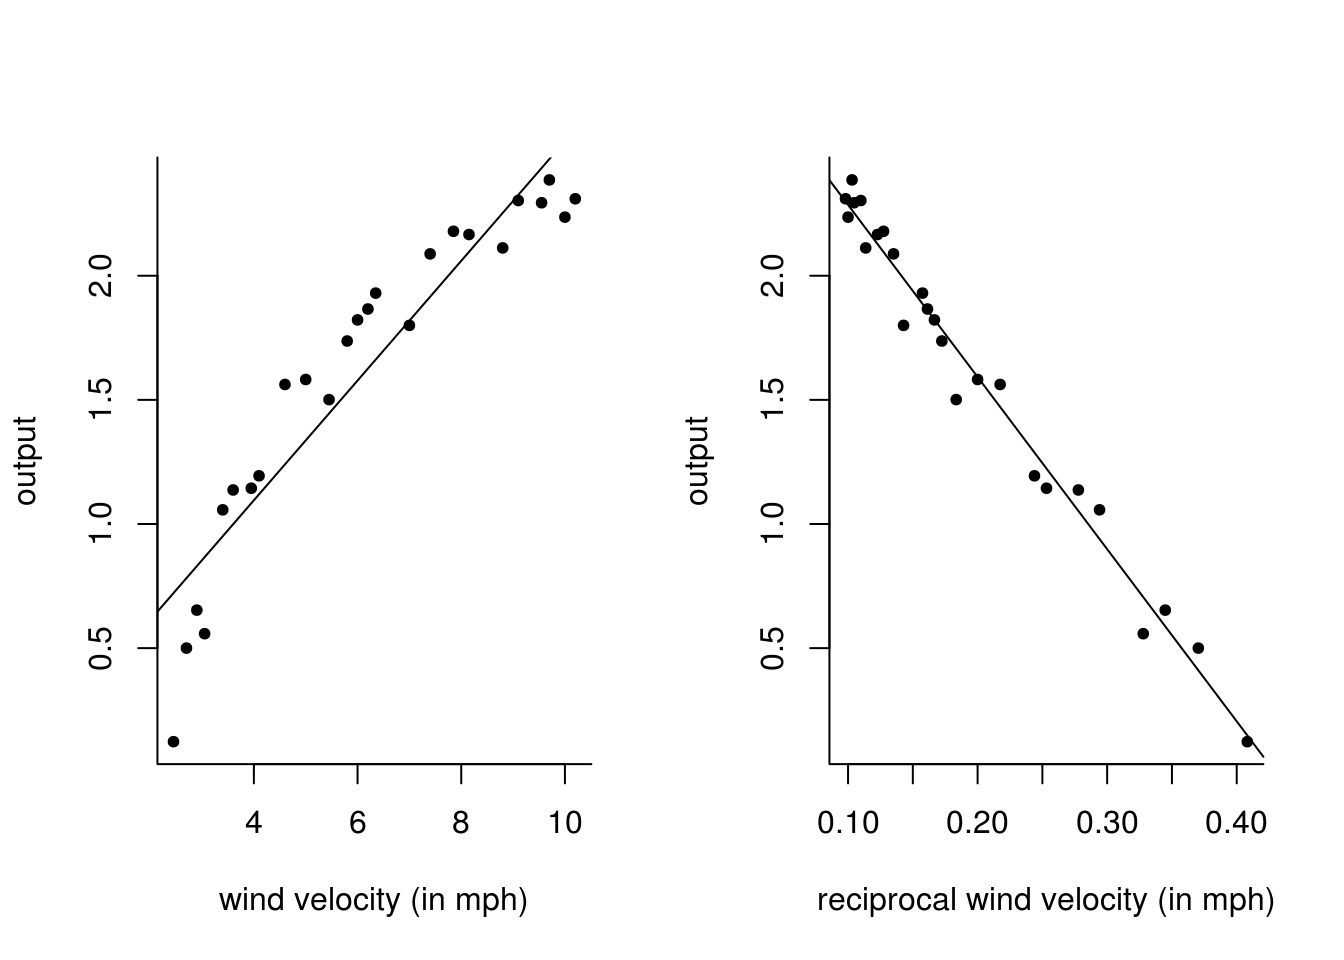
\includegraphics[width=0.7\linewidth]{LineaRModels_files/figure-latex/unnamed-chunk-26-1} \end{center}

\begin{Shaded}
\begin{Highlighting}[]
\CommentTok{#Standardized residuals r - manual calculation}
\CommentTok{#Standard deviation of errors}
\NormalTok{s <-}\StringTok{ }\KeywordTok{sqrt}\NormalTok{(}\KeywordTok{sum}\NormalTok{(}\KeywordTok{resid}\NormalTok{(lm_wind1)}\OperatorTok{^}\DecValTok{2}\NormalTok{)}\OperatorTok{/}\NormalTok{lm_wind1}\OperatorTok{$}\NormalTok{df.residual)}
\CommentTok{#Design matrix i.e. cbind(1, velocity)}
\NormalTok{Xmat1 <-}\StringTok{ }\KeywordTok{model.matrix}\NormalTok{(lm_wind1)}
\CommentTok{#Dimensions}
\NormalTok{n <-}\StringTok{ }\KeywordTok{nrow}\NormalTok{(Xmat1)}
\NormalTok{p <-}\StringTok{ }\KeywordTok{ncol}\NormalTok{(Xmat1)}
\CommentTok{#Projection matrix onto Xmat1}
\NormalTok{Hmat1 <-}\StringTok{ }\NormalTok{Xmat1 }\OperatorTok\StringTok{ }\KeywordTok{solve}\NormalTok{(}\KeywordTok{crossprod}\NormalTok{(Xmat1)) }\OperatorTok\StringTok{ }\KeywordTok{t}\NormalTok{(Xmat1)}
\CommentTok{#Diagonal of H}
\NormalTok{leverage <-}\StringTok{ }\KeywordTok{diag}\NormalTok{(Hmat1)}
\CommentTok{#Standardized residuals}
\NormalTok{r_wind1 <-}\StringTok{ }\KeywordTok{resid}\NormalTok{(lm_wind1)}\OperatorTok{/}\NormalTok{(s}\OperatorTok{*}\KeywordTok{sqrt}\NormalTok{(}\DecValTok{1}\OperatorTok{-}\NormalTok{leverage))}
\CommentTok{#The function rstandard returns those for us}
\NormalTok{r_wind2 <-}\StringTok{ }\KeywordTok{rstandard}\NormalTok{(lm_wind2)}

\CommentTok{#Plot of standardized residuals vs fitted values}
\KeywordTok{plot}\NormalTok{(}\DataTypeTok{y =}\NormalTok{ r_wind1 }\OperatorTok{-}\StringTok{ }\KeywordTok{mean}\NormalTok{(r_wind1), }\DataTypeTok{x =} \KeywordTok{fitted}\NormalTok{(lm_wind1), }
     \DataTypeTok{ylab =} \StringTok{"Standardized residuals"}\NormalTok{, }\DataTypeTok{xlab =} \StringTok{"Fitted values"}\NormalTok{, }
     \DataTypeTok{main =} \StringTok{"Residuals vs}\CharTok{\textbackslash{}n}\StringTok{fitted values"}\NormalTok{, }\DataTypeTok{sub =}\StringTok{"output ~ velocity"}\NormalTok{)}
\KeywordTok{abline}\NormalTok{(}\DataTypeTok{h =} \DecValTok{0}\NormalTok{, }\DataTypeTok{lty =} \DecValTok{2}\NormalTok{)}
\KeywordTok{plot}\NormalTok{(}\DataTypeTok{y =}\NormalTok{ r_wind2 }\OperatorTok{-}\StringTok{ }\KeywordTok{mean}\NormalTok{(r_wind2), }\DataTypeTok{x =} \KeywordTok{fitted}\NormalTok{(lm_wind2), }
     \DataTypeTok{ylab =} \StringTok{"Standardized residuals"}\NormalTok{, }\DataTypeTok{xlab =} \StringTok{"Fitted values"}\NormalTok{, }
     \DataTypeTok{main =} \StringTok{"Residuals vs}\CharTok{\textbackslash{}n}\StringTok{fitted values"}\NormalTok{, }\DataTypeTok{sub =}\StringTok{"output ~ 1/velocity"}\NormalTok{)}
\KeywordTok{abline}\NormalTok{(}\DataTypeTok{h =} \DecValTok{0}\NormalTok{, }\DataTypeTok{lty =} \DecValTok{2}\NormalTok{)}
\end{Highlighting}
\end{Shaded}

\begin{center}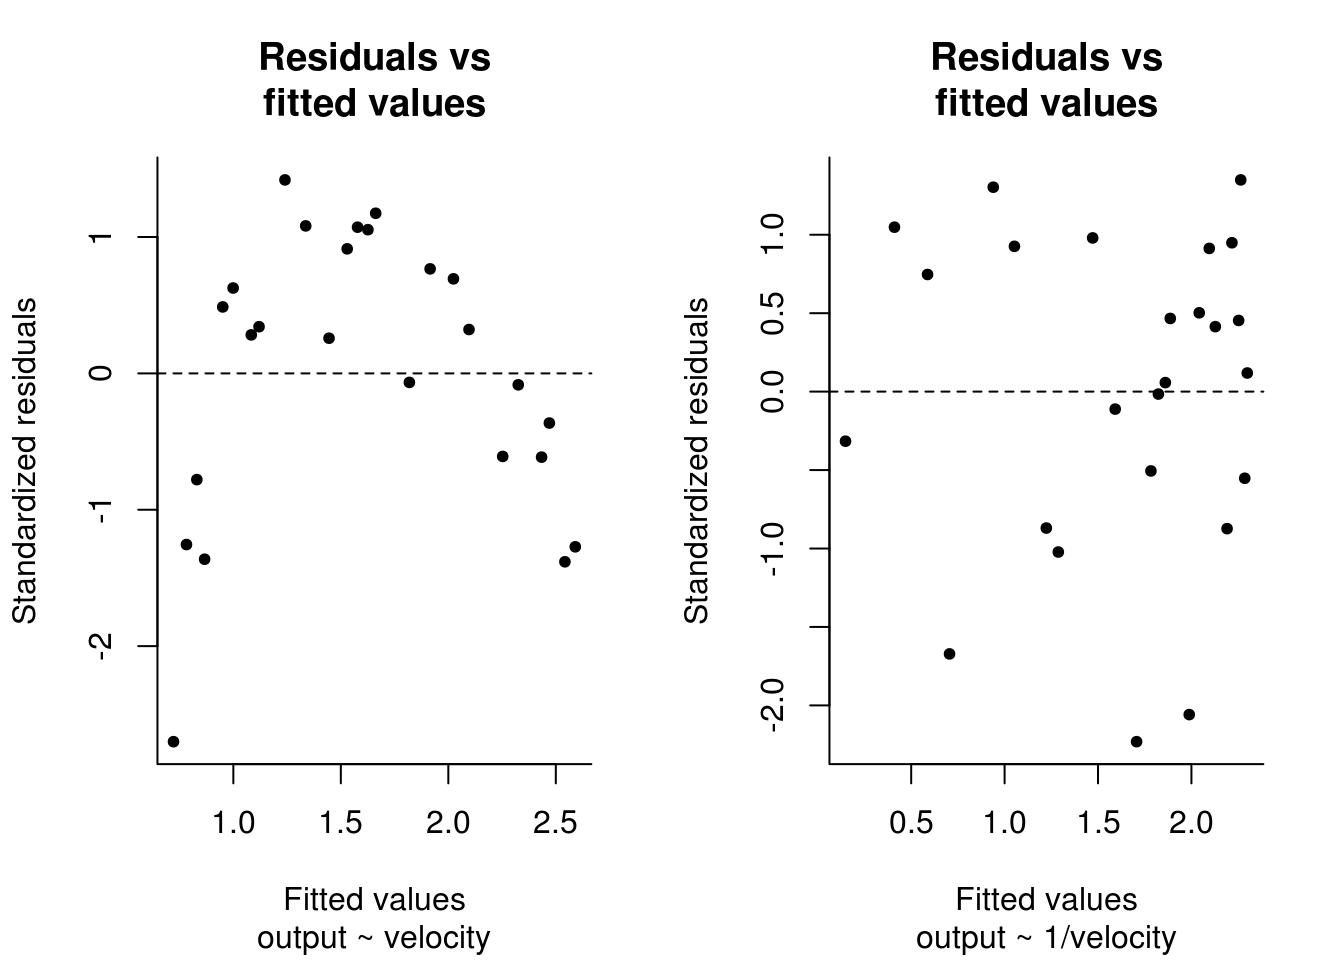
\includegraphics[width=0.7\linewidth]{LineaRModels_files/figure-latex/unnamed-chunk-26-2} \end{center}

There is some structure left in the model \texttt{output\ \textasciitilde{}\ velocity}, since the smallest values occur at the endpoint of the output. There is less visible structure in the model with the reciprocal.
The second model appears to fit better, since its \(\mathrm{R}^2\) value is 0.98 compared to 0.87 for the first model.
Note that, in the second model, the intercept corresponds to infinite strenght wind gusts.

\begin{Shaded}
\begin{Highlighting}[]
\CommentTok{#Predict new observation}
\NormalTok{pred1int <-}\StringTok{ }\KeywordTok{predict}\NormalTok{(lm_wind1, }\DataTypeTok{newdata =} \KeywordTok{data.frame}\NormalTok{(}\DataTypeTok{velocity =} \DecValTok{5}\NormalTok{), }
                    \DataTypeTok{interval =} \StringTok{"prediction"}\NormalTok{)}
\NormalTok{pred2int <-}\StringTok{ }\KeywordTok{predict}\NormalTok{(lm_wind2, }\DataTypeTok{newdata =} \KeywordTok{data.frame}\NormalTok{(}\DataTypeTok{recip_velo =} \DecValTok{1}\OperatorTok{/}\DecValTok{5}\NormalTok{), }
                    \DataTypeTok{interval =} \StringTok{"prediction"}\NormalTok{)}
\CommentTok{#Manually, see slide 68}
\NormalTok{xplus <-}\StringTok{ }\KeywordTok{c}\NormalTok{(}\DecValTok{1}\NormalTok{, }\DecValTok{5}\NormalTok{)}
\NormalTok{pred1 <-}\StringTok{ }\NormalTok{xplus }\OperatorTok\StringTok{ }\KeywordTok{coef}\NormalTok{(lm_wind1)}
\NormalTok{interv_length <-}\StringTok{ }\KeywordTok{qt}\NormalTok{(}\FloatTok{0.975}\NormalTok{, lm_wind1}\OperatorTok{$}\NormalTok{df.residual) }\OperatorTok{*}\StringTok{ }\NormalTok{summ1}\OperatorTok{$}\NormalTok{sigma }\OperatorTok{*}\StringTok{ }
\StringTok{            }\KeywordTok{sqrt}\NormalTok{((}\DecValTok{1} \OperatorTok{+}\StringTok{ }\KeywordTok{t}\NormalTok{(xplus) }\OperatorTok\StringTok{ }\KeywordTok{solve}\NormalTok{(}\KeywordTok{crossprod}\NormalTok{(Xmat1)) }\OperatorTok\StringTok{ }\NormalTok{xplus))}
\CommentTok{#Check that the calculation is correct}
\KeywordTok{isTRUE}\NormalTok{(}\KeywordTok{all.equal}\NormalTok{(}\KeywordTok{c}\NormalTok{(pred1, pred1 }\OperatorTok{-}\StringTok{ }\NormalTok{interv_length, pred1 }\OperatorTok{+}\StringTok{ }\NormalTok{interv_length), }
                 \KeywordTok{c}\NormalTok{(pred1int), }\DataTypeTok{check.attributes =} \OtherTok{FALSE}\NormalTok{))}
\end{Highlighting}
\end{Shaded}

\begin{verbatim}
## [1] TRUE
\end{verbatim}

The predicted output is 1.34 units of electrity for the first model, while the point forecast is 1.59 for the model with the reciprocal velocity. Both intervals overlap, but the second one {[}1.39, 1.79{]} is considerable narrower than the first one, given by {[}0.84, 1.84{]}.

\begin{Shaded}
\begin{Highlighting}[]
\KeywordTok{summary}\NormalTok{(}\KeywordTok{update}\NormalTok{(lm_wind1, . }\OperatorTok{~}\StringTok{ }\NormalTok{.}\OperatorTok{-}\DecValTok{1}\NormalTok{))}
\end{Highlighting}
\end{Shaded}

\begin{verbatim}
## 
## Call:
## lm(formula = output ~ velocity - 1)
## 
## Residuals:
##      Min       1Q   Median       3Q      Max 
## -0.51276 -0.17156  0.08675  0.20282  0.36832 
## 
## Coefficients:
##          Estimate Std. Error t value Pr(>|t|)
## velocity  0.25949    0.00715   36.29   <2e-16
## 
## Residual standard error: 0.2364 on 24 degrees of freedom
## Multiple R-squared:  0.9821, Adjusted R-squared:  0.9814 
## F-statistic:  1317 on 1 and 24 DF,  p-value: < 2.2e-16
\end{verbatim}

The function \texttt{update} changes the arguments of the linear model. Here, the \texttt{.} means keep all variables on lhs or rhs. You can also use it with a dataset to fit all the remaining variables after specifying the response variable, like for example \texttt{lm(output\ \textasciitilde{}\ .,\ \ data\ =\ windmill)} would have \texttt{velocity} as covariate.

We notice first that the confidence interval for \(\beta_0\), the intercept, includes zero, we cannot reject the null hypothesis that \(\beta_0=0\) at level \(0.95\).

The coefficient \(\beta_1\) corresponding to the effect of velocity has a smaller standard error than the first model. Does this make sense? If a model is correctly specified, addition of new variables that are unrelated does not introduce bias, but ncessarily inflates the standard errors by Gauss--Markov theorem. However, if the intercept should truly be there (this can be made necessary because of measurement errors) and \(\beta_0 \neq 0\), then the tests and confidence intervals will be invalid in the simplified model.

The multiple \(\mathrm{R}^2_c\) goes up the roof, but makes no sense here because it compares two models that are not nested (the model with a single mean versus which has no constant). A consequence of the removal of the intercept is that the average of the residuals is not zero anymore and that R returns different values for the \texttt{Multiple\ R-squared}.

\BeginKnitrBlock{rmdnote}
If you remove the intercept in a \texttt{lm} object using \texttt{-1}, the value returned by \texttt{summary} for the coefficient \texttt{Multiple\ R-squared} is the \(R^2\), not \(R^2_c\)!
\EndKnitrBlock{rmdnote}

We now produce the quantile-quantile plots using the results described in Section \ref{qqplot}.

\begin{Shaded}
\begin{Highlighting}[]
\NormalTok{Q <-}\StringTok{ }\KeywordTok{t}\NormalTok{(}\KeywordTok{qr.Q}\NormalTok{(}\KeywordTok{qr}\NormalTok{(Xmat1), }\DataTypeTok{complete =} \OtherTok{TRUE}\NormalTok{))}
\NormalTok{resQ1 <-}\StringTok{ }\NormalTok{(}\KeywordTok{t}\NormalTok{(Q) }\OperatorTok\StringTok{ }\KeywordTok{resid}\NormalTok{(lm_wind1))[}\OperatorTok{-}\NormalTok{(}\DecValTok{1}\OperatorTok{:}\DecValTok{2}\NormalTok{)]}
\CommentTok{#Function to add confidence intervals using order statitics}
\NormalTok{confint.qqplot.ptw <-}\StringTok{ }\ControlFlowTok{function}\NormalTok{(n, }\DataTypeTok{dist =} \StringTok{"norm"}\NormalTok{, ...)\{}
  \KeywordTok{t}\NormalTok{(}\KeywordTok{sapply}\NormalTok{(}\DecValTok{1}\OperatorTok{:}\NormalTok{n, }\ControlFlowTok{function}\NormalTok{(i)\{}
  \CommentTok{#Beta order statistic quantiles, mapped to scale dist}
    \KeywordTok{do.call}\NormalTok{(}\KeywordTok{paste0}\NormalTok{(}\StringTok{'q'}\NormalTok{, dist), }\KeywordTok{list}\NormalTok{(}\KeywordTok{qbeta}\NormalTok{(}\KeywordTok{c}\NormalTok{(}\FloatTok{0.025}\NormalTok{, }\FloatTok{0.975}\NormalTok{), i, n }\OperatorTok{-}\StringTok{ }\NormalTok{i }\OperatorTok{+}\StringTok{ }\DecValTok{1}\NormalTok{), ...))}
\NormalTok{  \}))}
\NormalTok{\}}

\CommentTok{# Adjust the number of observations}
\NormalTok{N <-}\StringTok{ }\NormalTok{n }\OperatorTok{-}\StringTok{ }\NormalTok{p}
\CommentTok{#Plotting positions on X axis}
\NormalTok{rankit <-}\StringTok{ }\KeywordTok{qnorm}\NormalTok{((}\DecValTok{1}\OperatorTok{:}\NormalTok{N) }\OperatorTok{/}\StringTok{ }\NormalTok{(N}\OperatorTok{+}\DecValTok{1}\NormalTok{))}
\KeywordTok{plot}\NormalTok{(rankit, }\KeywordTok{sort}\NormalTok{(}\KeywordTok{scale}\NormalTok{(resQ1)), }\DataTypeTok{xlab =} \StringTok{"Theoretical quantiles"}\NormalTok{, }
    \DataTypeTok{ylab =} \StringTok{"Sample quantiles"}\NormalTok{, }\DataTypeTok{main =} \StringTok{"Normal Q-Q plot"}\NormalTok{)}
\KeywordTok{abline}\NormalTok{(}\DataTypeTok{a =} \DecValTok{0}\NormalTok{, }\DataTypeTok{b =} \DecValTok{1}\NormalTok{)}
\NormalTok{confint_ptwise <-}\StringTok{ }\KeywordTok{confint.qqplot.ptw}\NormalTok{(N)}
\KeywordTok{lines}\NormalTok{(rankit, confint_ptwise[,}\DecValTok{1}\NormalTok{], }\DataTypeTok{col =} \StringTok{"gray"}\NormalTok{, }\DataTypeTok{lty =} \DecValTok{2}\NormalTok{)}
\KeywordTok{lines}\NormalTok{(rankit, confint_ptwise[,}\DecValTok{2}\NormalTok{], }\DataTypeTok{col =} \StringTok{"gray"}\NormalTok{, }\DataTypeTok{lty =} \DecValTok{2}\NormalTok{)}
\end{Highlighting}
\end{Shaded}

\begin{center}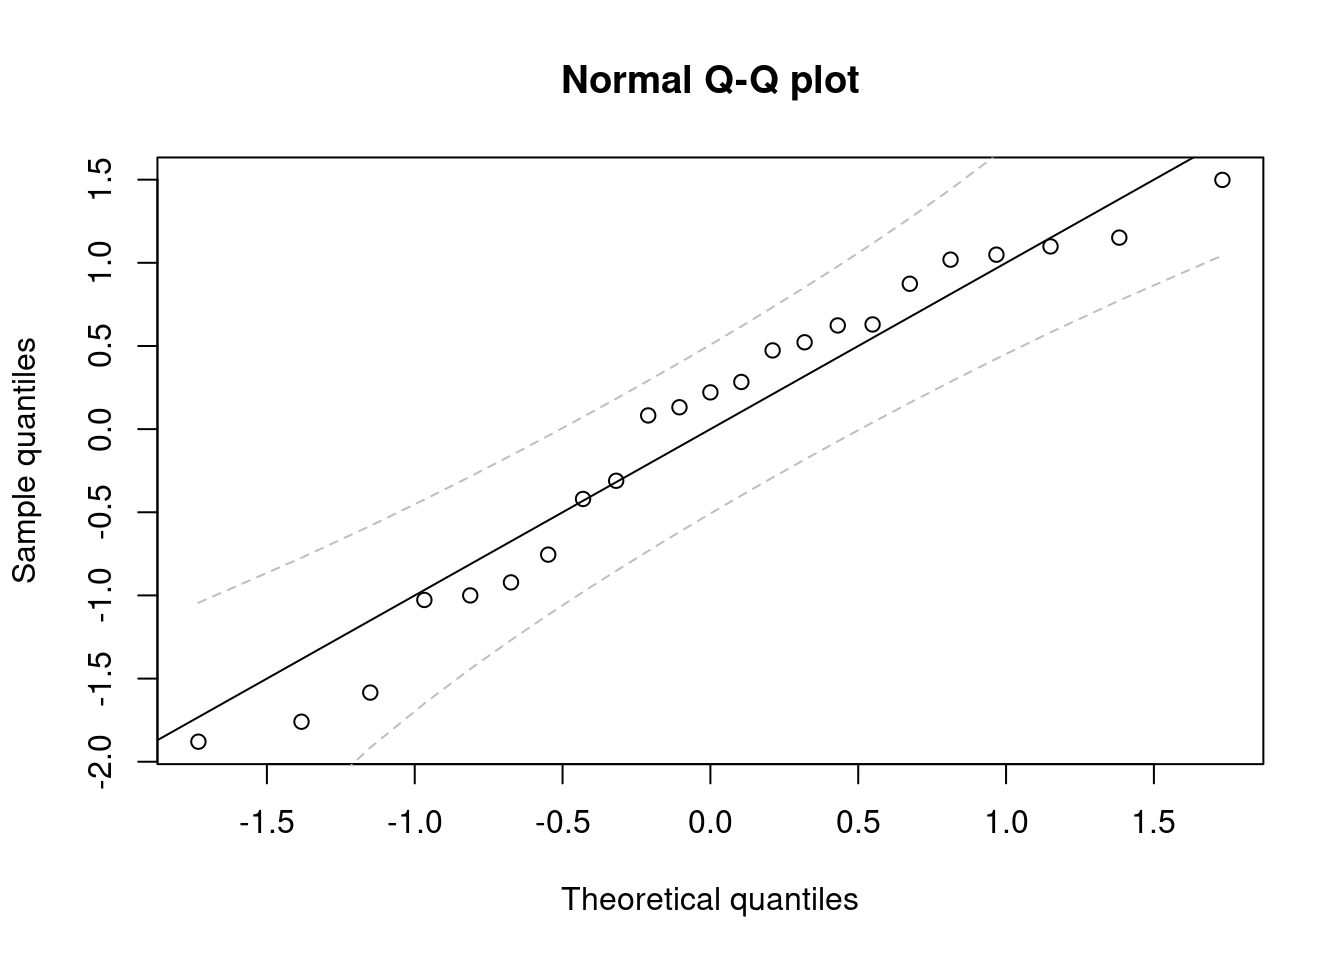
\includegraphics[width=0.7\linewidth]{LineaRModels_files/figure-latex/confints-1} \end{center}

\begin{Shaded}
\begin{Highlighting}[]
\NormalTok{boot_samps <-}\StringTok{ }\KeywordTok{replicate}\NormalTok{(}\KeywordTok{sort}\NormalTok{(}\KeywordTok{scale}\NormalTok{(}\KeywordTok{rnorm}\NormalTok{(N))), }\DataTypeTok{n =}\NormalTok{ (B <-}\StringTok{ }\DecValTok{9999}\NormalTok{))}
\NormalTok{alpha <-}\StringTok{ }\FloatTok{0.05}
\NormalTok{k <-}\StringTok{ }\NormalTok{alpha}\OperatorTok{/}\DecValTok{2}\OperatorTok{*}\NormalTok{(B }\OperatorTok{+}\StringTok{ }\DecValTok{1}\NormalTok{)}
\NormalTok{confint_boot <-}\StringTok{ }\KeywordTok{apply}\NormalTok{(boot_samps, }\DecValTok{1}\NormalTok{, sort)[}\KeywordTok{c}\NormalTok{(k, B}\OperatorTok{+}\DecValTok{1}\OperatorTok{-}\NormalTok{k),]}

\CommentTok{#Example with second model}
\NormalTok{Xmat2 <-}\StringTok{ }\KeywordTok{cbind}\NormalTok{(}\DecValTok{1}\NormalTok{, }\DecValTok{1}\OperatorTok{/}\NormalTok{velocity)}
\NormalTok{Q <-}\StringTok{ }\KeywordTok{t}\NormalTok{(}\KeywordTok{qr.Q}\NormalTok{(}\KeywordTok{qr}\NormalTok{(Xmat2), }\DataTypeTok{complete =} \OtherTok{TRUE}\NormalTok{))}
\NormalTok{resQ2 <-}\StringTok{ }\NormalTok{(}\KeywordTok{t}\NormalTok{(Q) }\OperatorTok\StringTok{ }\KeywordTok{resid}\NormalTok{(lm_wind2))[}\OperatorTok{-}\NormalTok{(}\DecValTok{1}\OperatorTok{:}\DecValTok{2}\NormalTok{)]}

\KeywordTok{plot}\NormalTok{(rankit, }\KeywordTok{sort}\NormalTok{(}\KeywordTok{scale}\NormalTok{(resQ2)), }\DataTypeTok{xlab =} \StringTok{"Theoretical quantiles"}\NormalTok{, }
    \DataTypeTok{ylab =} \StringTok{"Sample quantiles"}\NormalTok{, }\DataTypeTok{main =} \StringTok{"Normal Q-Q plot"}\NormalTok{)}
\KeywordTok{abline}\NormalTok{(}\DataTypeTok{a =} \DecValTok{0}\NormalTok{, }\DataTypeTok{b =} \DecValTok{1}\NormalTok{)}
\NormalTok{confint_ptwise <-}\StringTok{ }\KeywordTok{confint.qqplot.ptw}\NormalTok{(N)}
\CommentTok{#Simulated pointwise bands}
\KeywordTok{lines}\NormalTok{(rankit, confint_boot[}\DecValTok{1}\NormalTok{,], }\DataTypeTok{col =} \StringTok{"red"}\NormalTok{, }\DataTypeTok{lty =} \DecValTok{3}\NormalTok{)}
\KeywordTok{lines}\NormalTok{(rankit, confint_boot[}\DecValTok{2}\NormalTok{,], }\DataTypeTok{col =} \StringTok{"red"}\NormalTok{, }\DataTypeTok{lty =} \DecValTok{3}\NormalTok{)}
\CommentTok{#Theoretical bands based on order statistics distribution}
\KeywordTok{lines}\NormalTok{(rankit, confint_ptwise[,}\DecValTok{1}\NormalTok{], }\DataTypeTok{col =} \StringTok{"gray"}\NormalTok{, }\DataTypeTok{lty =} \DecValTok{2}\NormalTok{)}
\KeywordTok{lines}\NormalTok{(rankit, confint_ptwise[,}\DecValTok{2}\NormalTok{], }\DataTypeTok{col =} \StringTok{"gray"}\NormalTok{, }\DataTypeTok{lty =} \DecValTok{2}\NormalTok{)}
\end{Highlighting}
\end{Shaded}

\begin{center}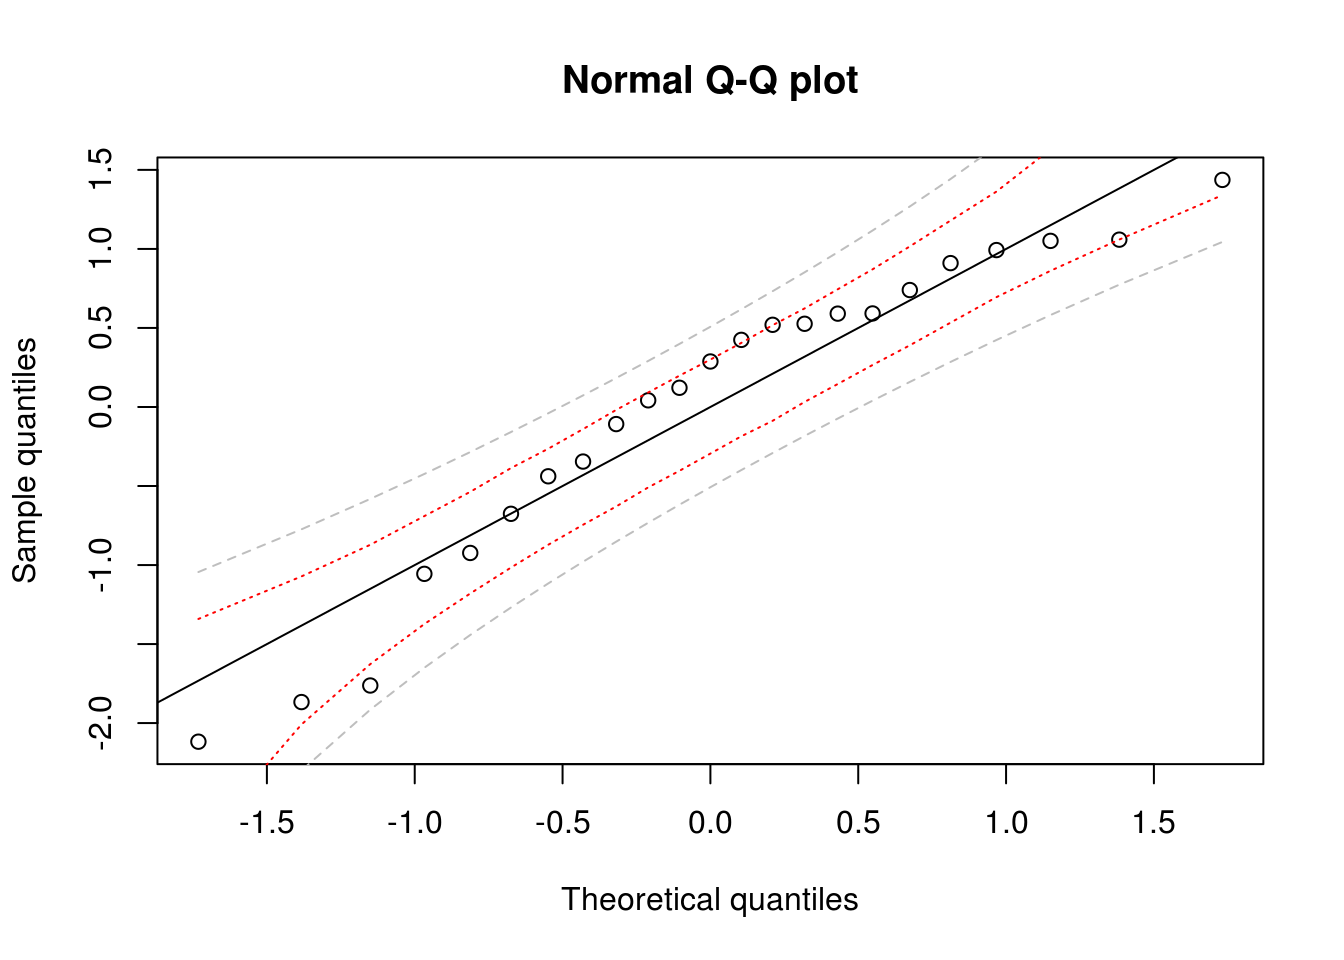
\includegraphics[width=0.7\linewidth]{LineaRModels_files/figure-latex/unnamed-chunk-28-1} \end{center}

The simulated pointwise confidence interval are shorter and account for the scaling.

\hypertarget{exercise-7.3---air-traffic}{%
\subsection{Exercise 7.3 - Air traffic}\label{exercise-7.3---air-traffic}}

First load the data set and plot the observations

\begin{Shaded}
\begin{Highlighting}[]
\KeywordTok{rm}\NormalTok{(}\DataTypeTok{list =} \KeywordTok{ls}\NormalTok{()) }\CommentTok{#clear environment }
\KeywordTok{par}\NormalTok{(}\DataTypeTok{bty =} \StringTok{"l"}\NormalTok{, }\DataTypeTok{pch =} \DecValTok{20}\NormalTok{)}
\NormalTok{url3 <-}\StringTok{ "https://lbelzile.bitbucket.io/math341/airpassengers.dat"}
\NormalTok{airpass <-}\StringTok{ }\KeywordTok{read.table}\NormalTok{(}\DataTypeTok{file =}\NormalTok{ url3, }\DataTypeTok{header =} \OtherTok{TRUE}\NormalTok{)}
\CommentTok{# Cast monthly binary to factor}
\NormalTok{airpass}\OperatorTok{$}\NormalTok{time <-}\StringTok{ }\NormalTok{airpass}\OperatorTok{$}\NormalTok{year }\OperatorTok{+}\StringTok{ }\NormalTok{(airpass}\OperatorTok{$}\NormalTok{month}\DecValTok{-1}\NormalTok{)}\OperatorTok{/}\DecValTok{12}
\NormalTok{airpass}\OperatorTok{$}\NormalTok{month <-}\StringTok{ }\KeywordTok{as.factor}\NormalTok{(airpass}\OperatorTok{$}\NormalTok{month)}
\KeywordTok{attach}\NormalTok{(airpass)}
\CommentTok{#Proceed as usual}
\KeywordTok{plot}\NormalTok{(}\DataTypeTok{y =}\NormalTok{ passengers, }\DataTypeTok{x =}\NormalTok{ time, }\DataTypeTok{type =} \StringTok{"l"}\NormalTok{,}
     \DataTypeTok{ylab =} \StringTok{"Monthly totals of international airline passengers (in thousands)"}\NormalTok{)}
\CommentTok{#Fit simple linear model with time as covariate}
\NormalTok{sum_ap <-}\StringTok{ }\KeywordTok{summary}\NormalTok{(fit_ap <-}\StringTok{ }\KeywordTok{lm}\NormalTok{(passengers }\OperatorTok{~}\StringTok{ }\NormalTok{time))}
\KeywordTok{lines}\NormalTok{(time, }\KeywordTok{fitted}\NormalTok{(fit_ap), }\DataTypeTok{col =} \DecValTok{2}\NormalTok{)}
\CommentTok{#Create monthly dummies}
\CommentTok{#create factor using `as.factor}
\NormalTok{month <-}\StringTok{ }\KeywordTok{as.factor}\NormalTok{(}\KeywordTok{rep}\NormalTok{(}\DecValTok{1}\OperatorTok{:}\DecValTok{12}\NormalTok{, }\DataTypeTok{length =} \KeywordTok{length}\NormalTok{(time)))}
\KeywordTok{levels}\NormalTok{(month) <-}\StringTok{ }\NormalTok{month.abb }\CommentTok{#abbreviation of months}
\CommentTok{#A fancier way would convert the fraction to units, }
\CommentTok{#month <- as.factor(1 + as.integer(c(time*12) %% 12)) # %% is modulo operator}
\CommentTok{#quarter <- as.factor(rep(1:4, each = 3, length = length(time)))}
\NormalTok{sum_ad <-}\StringTok{ }\KeywordTok{summary}\NormalTok{(fit_ad <-}\StringTok{ }\KeywordTok{lm}\NormalTok{(passengers }\OperatorTok{~}\StringTok{ }\NormalTok{time }\OperatorTok{+}\StringTok{ }\NormalTok{month))}
\KeywordTok{lines}\NormalTok{(time, }\KeywordTok{fitted}\NormalTok{(fit_ad), }\DataTypeTok{lty =} \DecValTok{2}\NormalTok{, }\DataTypeTok{col =} \DecValTok{4}\NormalTok{) }\CommentTok{#dashed blue line}
\end{Highlighting}
\end{Shaded}

\begin{center}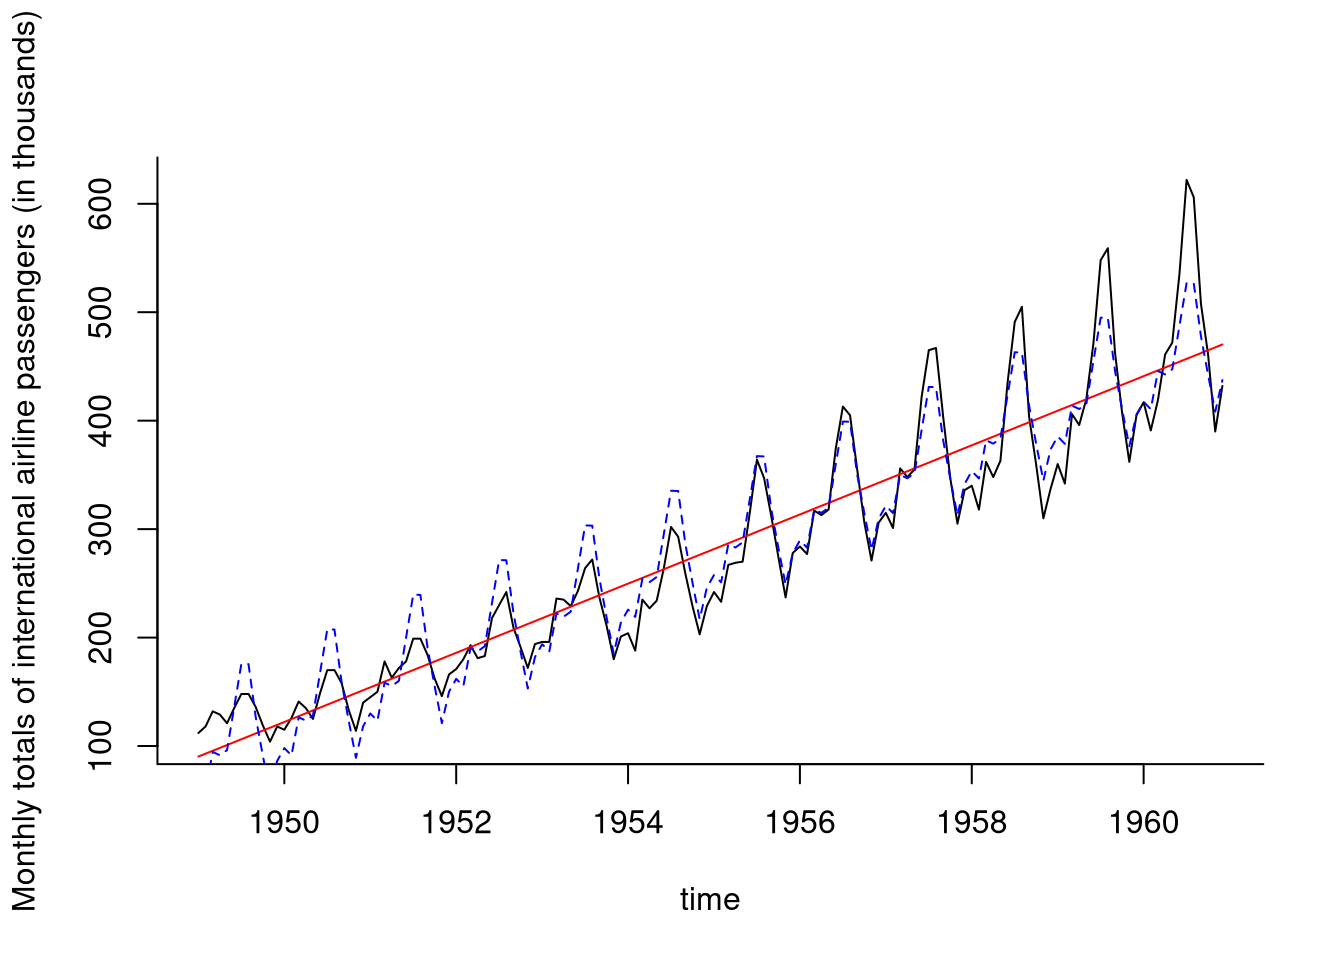
\includegraphics[width=0.7\linewidth]{LineaRModels_files/figure-latex/unnamed-chunk-29-1} \end{center}

\begin{Shaded}
\begin{Highlighting}[]
\CommentTok{#Prediction }
\KeywordTok{predict}\NormalTok{(fit_ad, }\DataTypeTok{newdata =} \KeywordTok{data.frame}\NormalTok{(}\DataTypeTok{time =} \DecValTok{1962}\OperatorTok{+}\DecValTok{11}\OperatorTok{/}\DecValTok{12}\NormalTok{, }\DataTypeTok{month =}\NormalTok{ month[}\DecValTok{12}\NormalTok{]))}
\end{Highlighting}
\end{Shaded}

\begin{verbatim}
##       1 
## 501.263
\end{verbatim}

\begin{Shaded}
\begin{Highlighting}[]
\KeywordTok{coef}\NormalTok{(fit_ad) }\OperatorTok\StringTok{ }\KeywordTok{c}\NormalTok{(}\DecValTok{1}\NormalTok{, }\DecValTok{1962} \OperatorTok{+}\StringTok{ }\DecValTok{11}\OperatorTok{/}\DecValTok{12}\NormalTok{, }\KeywordTok{rep}\NormalTok{(}\DecValTok{0}\NormalTok{, }\DecValTok{10}\NormalTok{), }\DecValTok{1}\NormalTok{) }\CommentTok{#baseline is January if global mean included}
\end{Highlighting}
\end{Shaded}

\begin{verbatim}
##         [,1]
## [1,] 501.263
\end{verbatim}

We notice that the model does an overall good job at getting the big features, but misses many things. The first point is that the relationship is not quite linear: a residual plot shows a somewhat quadratic relation between the fitted values and the residuals. The second obvious feature not captured is the change in the variation (the amplitude of the wave pattern changes over time). Since the variance is increasing, a log-transformation may help stabilize it.
The residuals are not apparently close to normal (the last values are systematically too large) and there is some skewness. The last few points have large leverage and drive the curve up.

\begin{Shaded}
\begin{Highlighting}[]
\NormalTok{n <-}\StringTok{ }\KeywordTok{length}\NormalTok{(passengers)}
\NormalTok{p <-}\StringTok{ }\KeywordTok{length}\NormalTok{(}\KeywordTok{coef}\NormalTok{(fit_ad)) }
\KeywordTok{par}\NormalTok{(}\DataTypeTok{mfrow =} \KeywordTok{c}\NormalTok{(}\DecValTok{2}\NormalTok{, }\DecValTok{2}\NormalTok{))}
\KeywordTok{plot}\NormalTok{(fit_ad, }\DataTypeTok{which =} \DecValTok{1}\NormalTok{) }\CommentTok{#residuals vs fitted values}
\KeywordTok{plot}\NormalTok{(fit_ad, }\DataTypeTok{which =} \DecValTok{2}\NormalTok{) }\CommentTok{#Normal Q-Q plot}
\KeywordTok{plot}\NormalTok{(fit_ad, }\DataTypeTok{which =} \DecValTok{3}\NormalTok{) }\CommentTok{#standardized residuals vs fitted values}
\KeywordTok{plot}\NormalTok{(fit_ad, }\DataTypeTok{which =} \DecValTok{4}\NormalTok{, }\DataTypeTok{sub.caption =} \StringTok{""}\NormalTok{) }\CommentTok{#Cook distance plot}
\KeywordTok{abline}\NormalTok{(}\DataTypeTok{h =} \DecValTok{8}\OperatorTok{/}\NormalTok{(n }\OperatorTok{-}\StringTok{ }\DecValTok{2}\OperatorTok{*}\NormalTok{p), }\DataTypeTok{col =} \DecValTok{2}\NormalTok{)}
\end{Highlighting}
\end{Shaded}

\begin{center}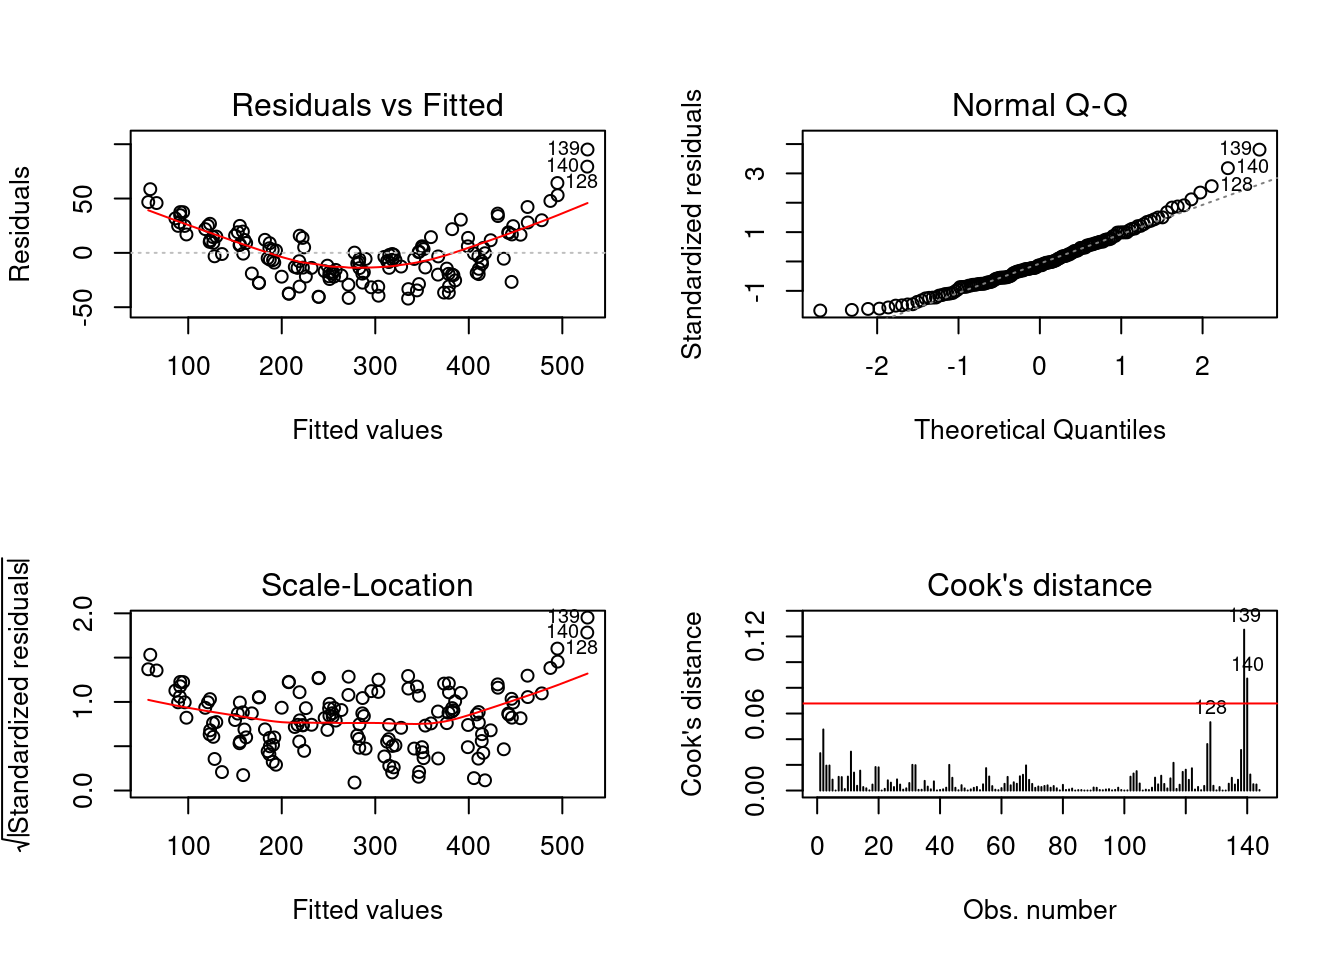
\includegraphics[width=0.7\linewidth]{LineaRModels_files/figure-latex/unnamed-chunk-30-1} \end{center}

\begin{Shaded}
\begin{Highlighting}[]
\KeywordTok{par}\NormalTok{(}\DataTypeTok{mfrow =} \KeywordTok{c}\NormalTok{(}\DecValTok{1}\NormalTok{, }\DecValTok{1}\NormalTok{)) }\CommentTok{#return to one plot per window}
\CommentTok{#Compute Cook statistic and other influence statistics}
\NormalTok{infl_ad <-}\StringTok{ }\KeywordTok{influence.measures}\NormalTok{(fit_ad)}
\NormalTok{cookval_ad <-}\StringTok{ }\NormalTok{infl_ad}\OperatorTok{$}\NormalTok{infmat[,}\StringTok{"cook.d"}\NormalTok{] }\CommentTok{#cooks.distance}
\CommentTok{#Diagonal values of the "hat" projection matrix}
\NormalTok{h_ad <-}\StringTok{ }\NormalTok{infl_ad}\OperatorTok{$}\NormalTok{infmat[, }\StringTok{"hat"}\NormalTok{] }\CommentTok{#hatvalues}
\KeywordTok{plot}\NormalTok{(time, }\KeywordTok{rstudent}\NormalTok{(fit_ad), }
     \DataTypeTok{ylab =} \StringTok{"Externally studentized residuals"}\NormalTok{, }
     \DataTypeTok{xlab =} \StringTok{"Time (in years)"}\NormalTok{)}
\end{Highlighting}
\end{Shaded}

\begin{center}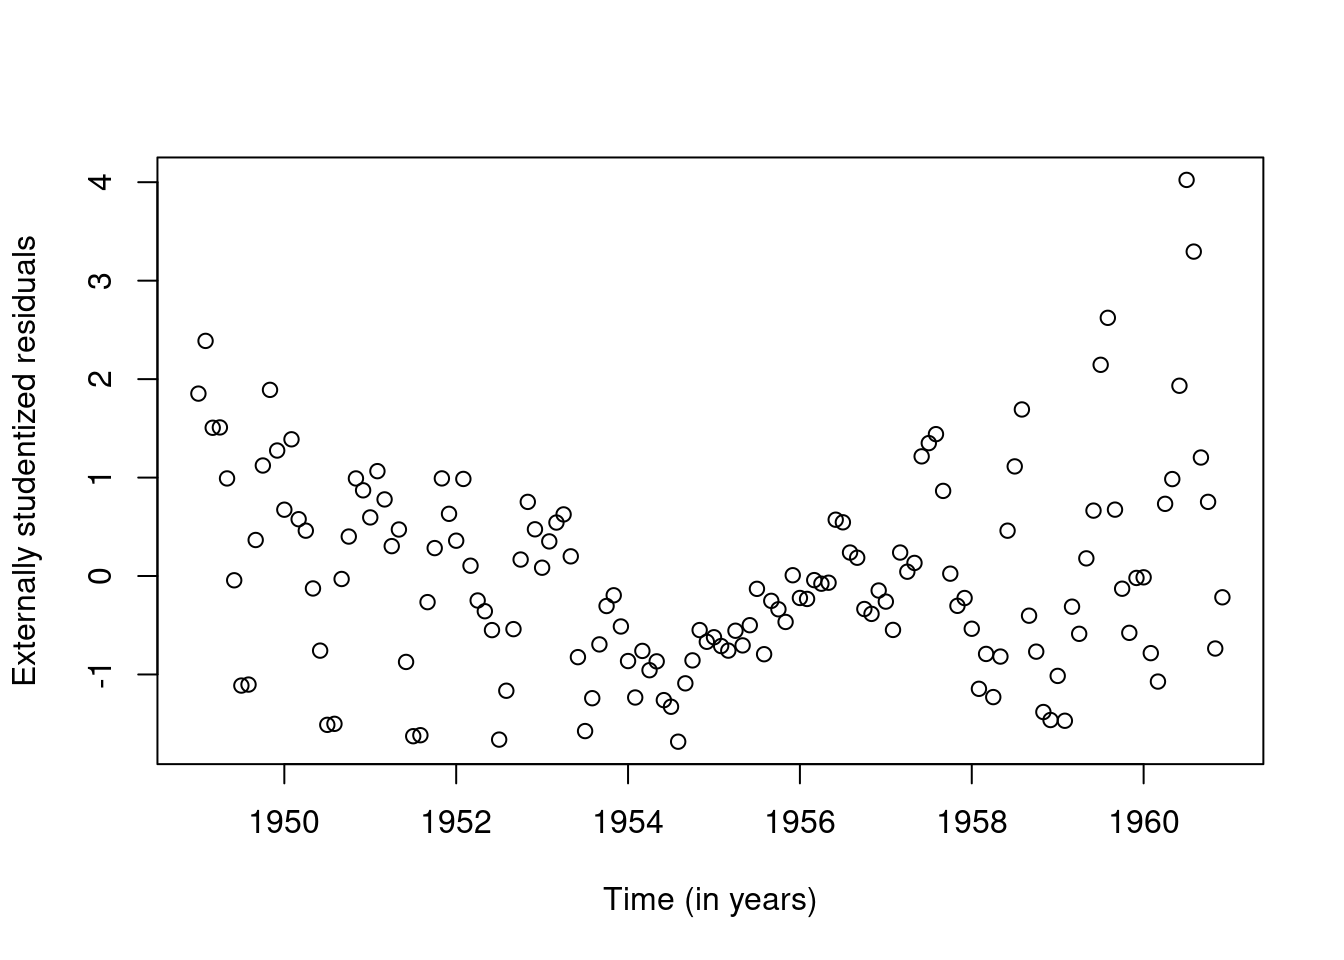
\includegraphics[width=0.7\linewidth]{LineaRModels_files/figure-latex/unnamed-chunk-30-2} \end{center}

Let us consider the log counts. The fit is much better and the quadratic relationship with the residuals vs fitted values is attenuated. While some points still have high leverage value, they are not considered outliers.

\begin{Shaded}
\begin{Highlighting}[]
\NormalTok{fit_l <-}\StringTok{ }\KeywordTok{lm}\NormalTok{(}\KeywordTok{log}\NormalTok{(passengers) }\OperatorTok{~}\StringTok{ }\NormalTok{time }\OperatorTok{+}\StringTok{ }\NormalTok{month)}
\KeywordTok{plot}\NormalTok{(}\KeywordTok{log}\NormalTok{(passengers) }\OperatorTok{~}\StringTok{ }\NormalTok{time, }\DataTypeTok{main =} \StringTok{"International airline passengers"}\NormalTok{,}
\DataTypeTok{ylab =} \StringTok{"log of monthly total count (in thousands)"}\NormalTok{, }\DataTypeTok{type =} \StringTok{"l"}\NormalTok{)}
\KeywordTok{lines}\NormalTok{(time, }\KeywordTok{fitted}\NormalTok{(fit_l), }\DataTypeTok{lty =} \DecValTok{2}\NormalTok{, }\DataTypeTok{col =} \DecValTok{4}\NormalTok{)}
\end{Highlighting}
\end{Shaded}

\begin{center}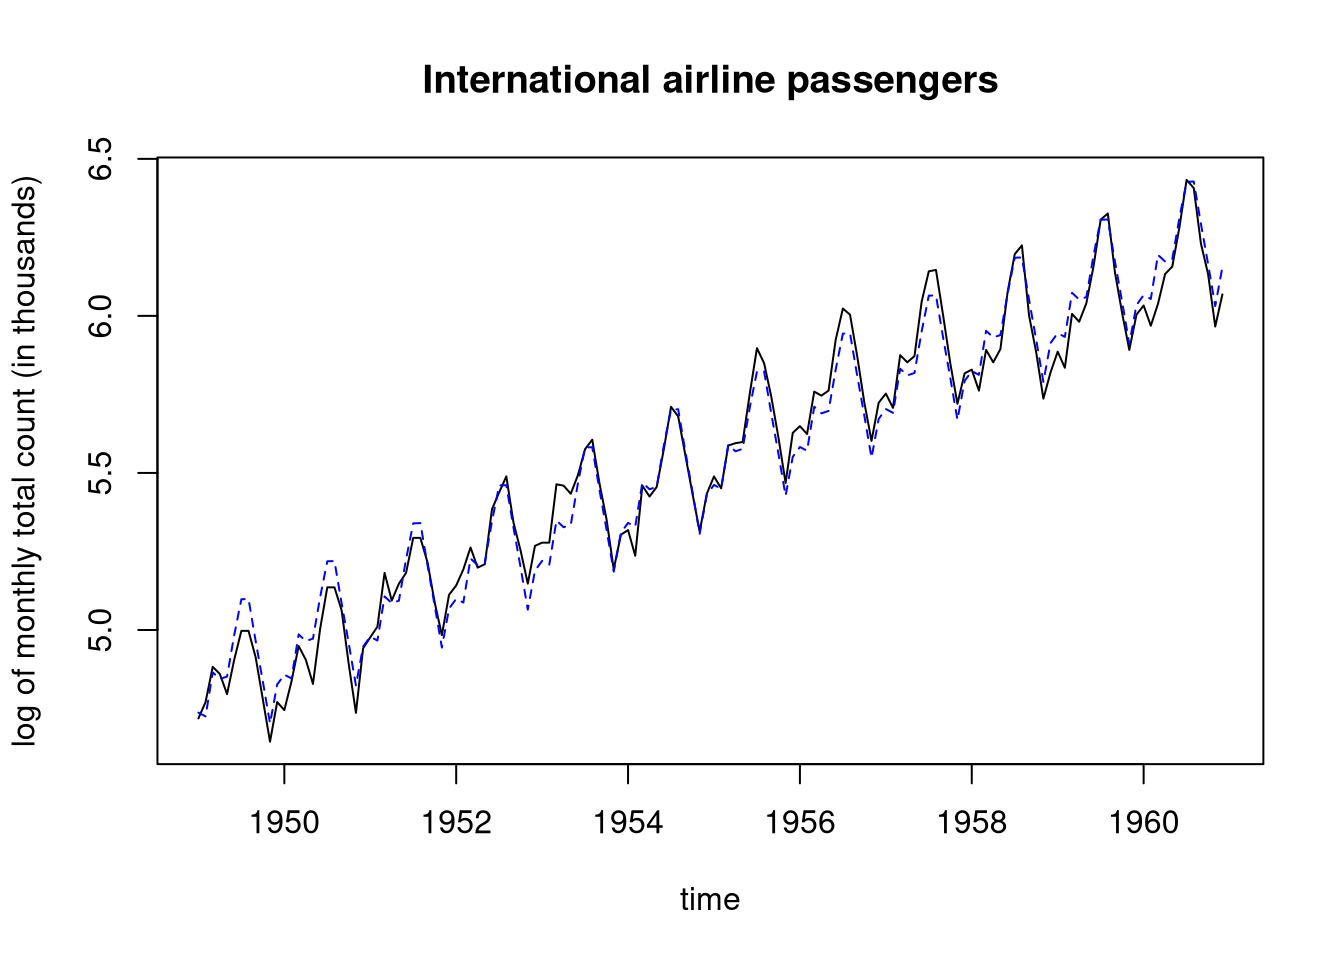
\includegraphics[width=0.7\linewidth]{LineaRModels_files/figure-latex/unnamed-chunk-31-1} \end{center}

\begin{Shaded}
\begin{Highlighting}[]
\KeywordTok{par}\NormalTok{(}\DataTypeTok{mfrow =} \KeywordTok{c}\NormalTok{(}\DecValTok{2}\NormalTok{, }\DecValTok{2}\NormalTok{), }\DataTypeTok{pch =} \DecValTok{20}\NormalTok{)}
\CommentTok{# Q-Q plot}
\KeywordTok{plot}\NormalTok{(}\DataTypeTok{x =} \KeywordTok{qt}\NormalTok{((}\DecValTok{1}\OperatorTok{:}\NormalTok{n)}\OperatorTok{/}\NormalTok{(n}\OperatorTok{+}\DecValTok{1}\NormalTok{), }\DataTypeTok{df =}\NormalTok{ n }\OperatorTok{-}\StringTok{ }\NormalTok{p }\OperatorTok{+}\StringTok{ }\DecValTok{1}\NormalTok{), }\DataTypeTok{y =} \KeywordTok{sort}\NormalTok{(}\KeywordTok{scale}\NormalTok{(}\KeywordTok{rstudent}\NormalTok{(fit_l))),}
     \DataTypeTok{xlab =} \StringTok{"Theoretical quantiles"}\NormalTok{, }\DataTypeTok{ylab =} \StringTok{"Empirical quantiles"}\NormalTok{,}
     \DataTypeTok{main =} \StringTok{"Quantile-quantile plot of}\CharTok{\textbackslash{}n}\StringTok{externally studentized residuals"}\NormalTok{)}
\KeywordTok{abline}\NormalTok{(}\DataTypeTok{a =} \DecValTok{0}\NormalTok{, }\DataTypeTok{b =} \DecValTok{1}\NormalTok{)}
\KeywordTok{plot}\NormalTok{(fit_l, }\DataTypeTok{which =} \DecValTok{1}\NormalTok{, }\DataTypeTok{sub.caption =} \StringTok{""}\NormalTok{)}
\KeywordTok{plot}\NormalTok{(fit_l, }\DataTypeTok{which =} \DecValTok{4}\NormalTok{, }\DataTypeTok{sub.caption =} \StringTok{""}\NormalTok{)}
\KeywordTok{abline}\NormalTok{(}\DataTypeTok{h =} \DecValTok{8}\OperatorTok{/}\NormalTok{(n }\OperatorTok{-}\StringTok{ }\DecValTok{2}\OperatorTok{*}\NormalTok{p), }\DataTypeTok{col =} \DecValTok{2}\NormalTok{)}
\end{Highlighting}
\end{Shaded}

\begin{center}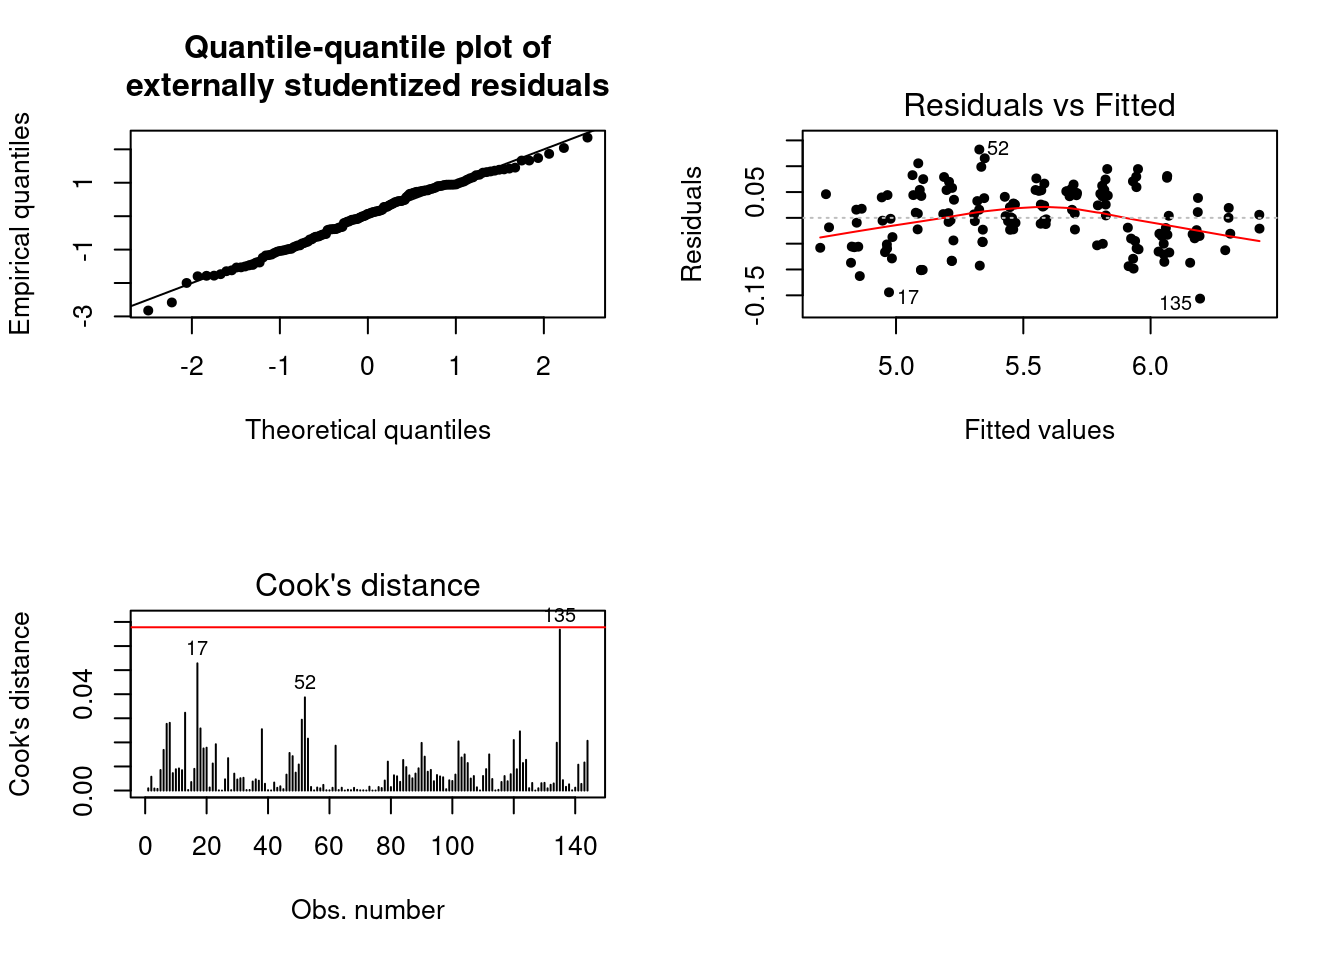
\includegraphics[width=0.7\linewidth]{LineaRModels_files/figure-latex/unnamed-chunk-31-2} \end{center}

One hypothesis of the linear model that is clearly violated here is the independence of the errors. Even if the variance \(\mathsf{Var}(\boldsymbol{e})=\sigma^2\mathbf{M}_{\mathbf{X}}\) need not have independent errors, there is positive dependence from residual to residual. This is confirmed by looking at the autocorrelation, which indicates geometric decay. This will be covered in MATH 342 (Time Series), but you should just think here of shocks carrying through until the next period before the model reverts to the mean.

Ignoring the serial dependence in the error has consequences: the standard errors are too small (since errors are correlated, there is less units of information so we are overconfident in our uncertainty quantification).

\begin{Shaded}
\begin{Highlighting}[]
\CommentTok{#Laggedresidual plots}
\KeywordTok{par}\NormalTok{(}\DataTypeTok{mfrow =} \KeywordTok{c}\NormalTok{(}\DecValTok{1}\NormalTok{, }\DecValTok{1}\NormalTok{))}
\KeywordTok{plot}\NormalTok{(}\DataTypeTok{x =} \KeywordTok{resid}\NormalTok{(fit_l)[}\OperatorTok{-}\DecValTok{1}\NormalTok{], }\DataTypeTok{y =} \KeywordTok{resid}\NormalTok{(fit_l)[}\OperatorTok{-}\NormalTok{n], }
  \DataTypeTok{ylab =} \KeywordTok{expression}\NormalTok{(}\KeywordTok{bold}\NormalTok{(e)[}\OperatorTok{-}\NormalTok{n]), }\DataTypeTok{xlab =} \KeywordTok{expression}\NormalTok{(}\KeywordTok{bold}\NormalTok{(e)[}\OperatorTok{-}\DecValTok{1}\NormalTok{]), }
  \DataTypeTok{main =} \StringTok{"Lagged residual plot"}\NormalTok{)}
\end{Highlighting}
\end{Shaded}

\begin{center}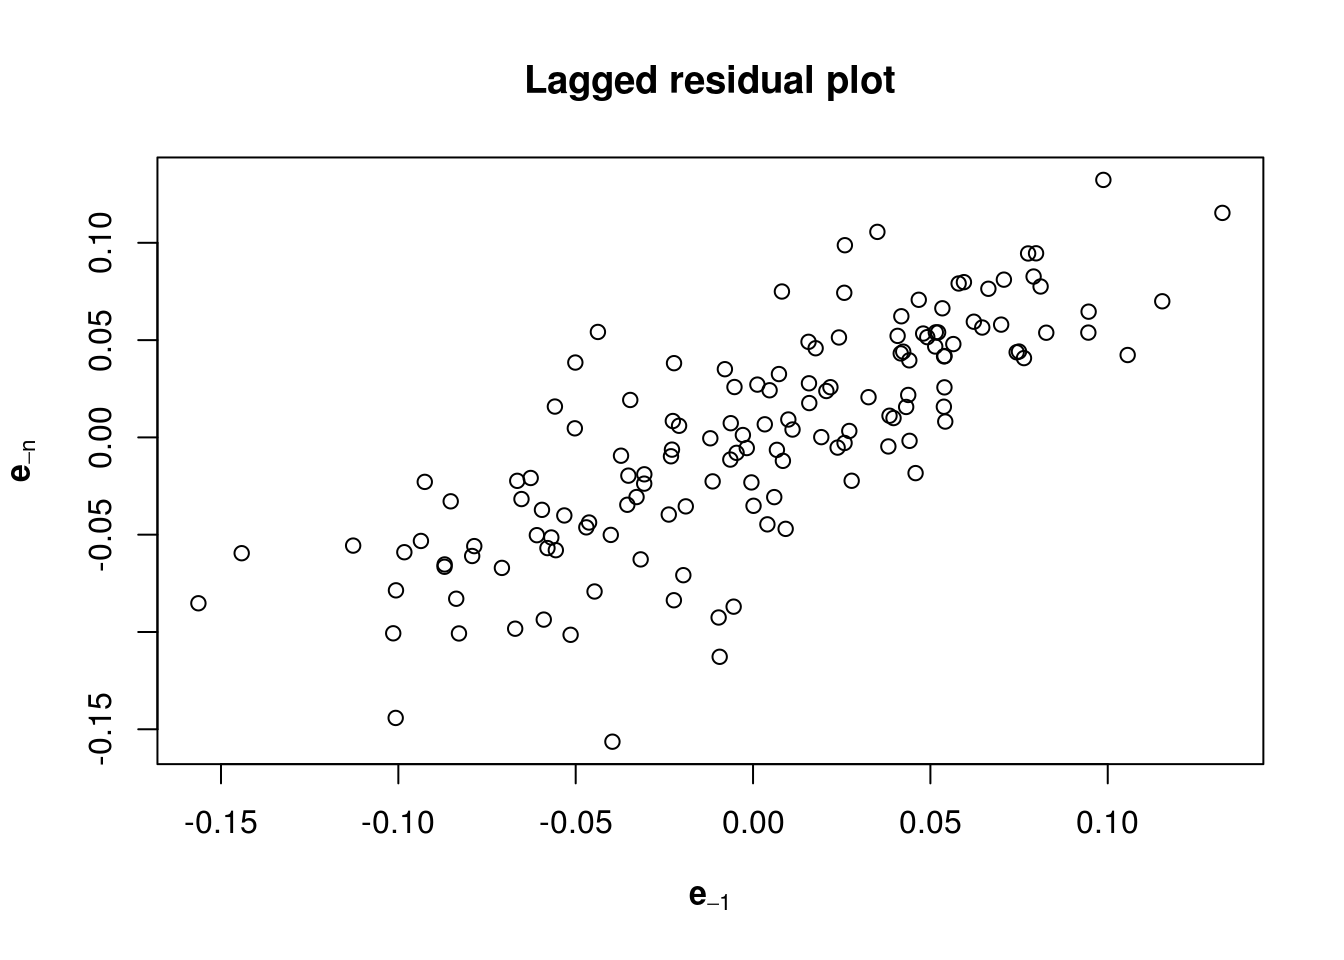
\includegraphics[width=0.7\linewidth]{LineaRModels_files/figure-latex/unnamed-chunk-32-1} \end{center}

\begin{Shaded}
\begin{Highlighting}[]
\CommentTok{#(partial) correlogram: if residuals have no structure}
\CommentTok{#there should not be anything outside the bands 19 times out of 20}
\CommentTok{#Covered in detail in MATH-342 (Time series)}
\KeywordTok{par}\NormalTok{(}\DataTypeTok{mfrow =} \KeywordTok{c}\NormalTok{(}\DecValTok{1}\NormalTok{, }\DecValTok{2}\NormalTok{))}
\KeywordTok{acf}\NormalTok{(}\KeywordTok{resid}\NormalTok{(fit_l), }\DataTypeTok{main =} \StringTok{"Autocorrelation of residuals"}\NormalTok{, }\DataTypeTok{xlim =} \KeywordTok{c}\NormalTok{(}\DecValTok{1}\NormalTok{,}\DecValTok{20}\NormalTok{))}
\KeywordTok{pacf}\NormalTok{(}\KeywordTok{resid}\NormalTok{(fit_l), }\DataTypeTok{main =} \StringTok{"Partial autocorrelation of residuals"}\NormalTok{)}
\end{Highlighting}
\end{Shaded}

\begin{center}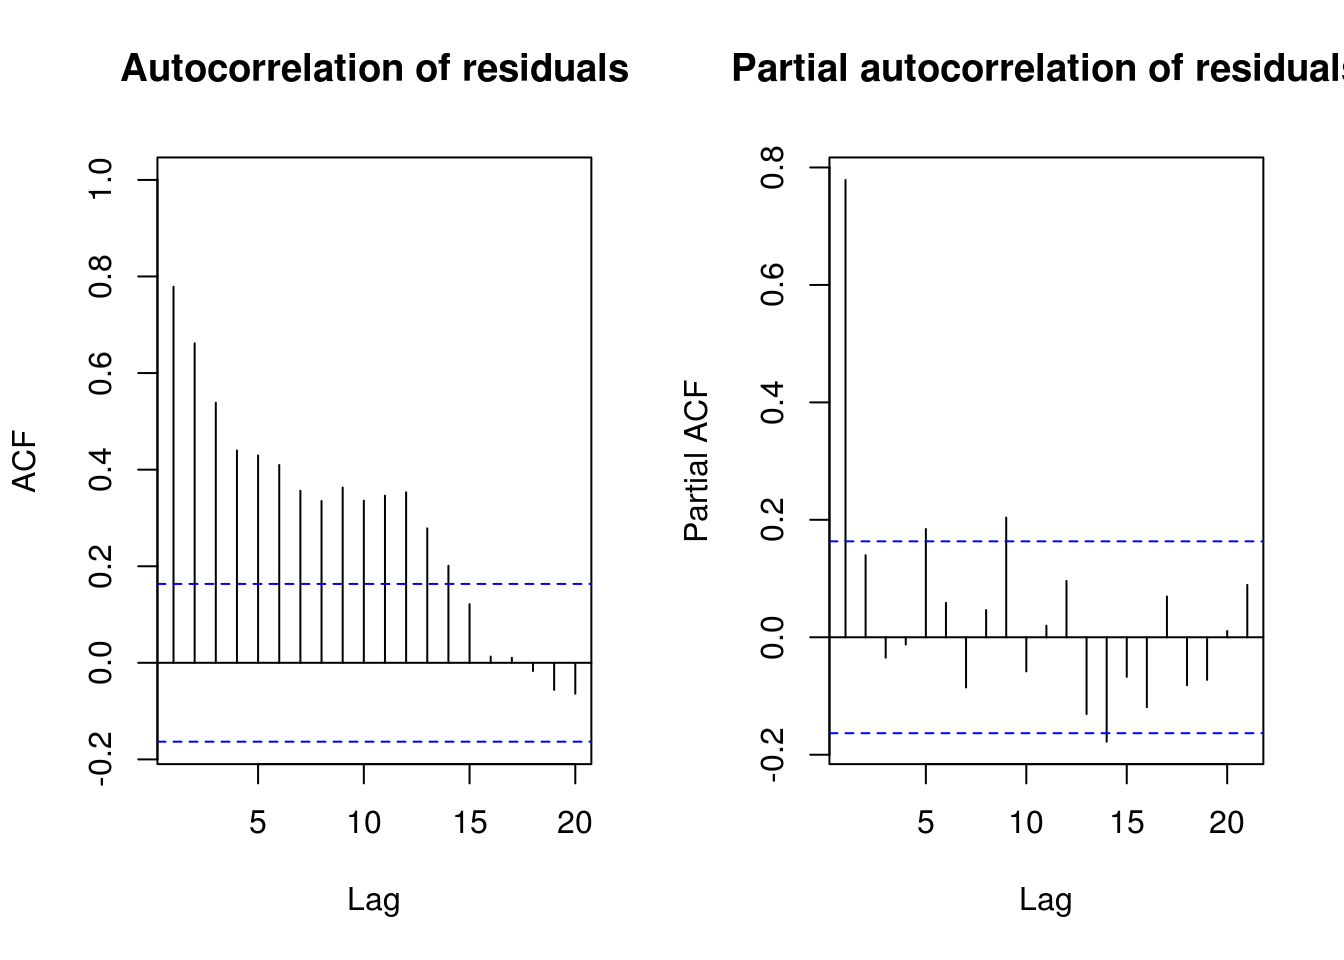
\includegraphics[width=0.7\linewidth]{LineaRModels_files/figure-latex/unnamed-chunk-32-2} \end{center}

\begin{Shaded}
\begin{Highlighting}[]
\CommentTok{#detach dataset}
\KeywordTok{detach}\NormalTok{(airpass)}
\end{Highlighting}
\end{Shaded}

\hypertarget{exercise-7.4---determinants-of-earnings}{%
\subsection{Exercise 7.4 - Determinants of earnings}\label{exercise-7.4---determinants-of-earnings}}

\begin{Shaded}
\begin{Highlighting}[]
\NormalTok{url4 <-}\StringTok{ "https://lbelzile.bitbucket.io/math341/labour.dat"}
\NormalTok{labour <-}\StringTok{ }\KeywordTok{read.table}\NormalTok{(url4, }\DataTypeTok{header =} \OtherTok{TRUE}\NormalTok{, }\DataTypeTok{stringsAsFactors =} \OtherTok{TRUE}\NormalTok{)}
\KeywordTok{attach}\NormalTok{(labour)}
\CommentTok{## Create dummy for extract columns}
\CommentTok{## additional years of schooling after high school}
\NormalTok{labour}\OperatorTok{$}\NormalTok{pseduc  <-}\StringTok{ }\KeywordTok{I}\NormalTok{(education }\OperatorTok{>=}\StringTok{ }\DecValTok{13}\NormalTok{) }\OperatorTok{*}\StringTok{ }\NormalTok{(education }\OperatorTok{-}\StringTok{ }\DecValTok{13}\NormalTok{)}
\NormalTok{educ_lm <-}\StringTok{ }\KeywordTok{lm}\NormalTok{(lhwages }\OperatorTok{~}\StringTok{ }\NormalTok{education }\OperatorTok{+}\StringTok{ }\NormalTok{pseduc, }\DataTypeTok{data =}\NormalTok{ labour)}
\KeywordTok{confint}\NormalTok{(educ_lm)}
\end{Highlighting}
\end{Shaded}

\begin{verbatim}
##                  2.5 %     97.5 %
## (Intercept) 2.29267414 2.51468758
## education   0.01030330 0.02940631
## pseduc      0.03325994 0.06318974
\end{verbatim}

\begin{Shaded}
\begin{Highlighting}[]
\CommentTok{## Plot with meaningful title + axis label}
\CommentTok{## red for Male, black for Female}
\KeywordTok{plot}\NormalTok{(lhwages }\OperatorTok{~}\StringTok{ }\NormalTok{education, }\DataTypeTok{pch =} \DecValTok{20}\NormalTok{, }\DataTypeTok{col =} \KeywordTok{as.integer}\NormalTok{(gender),}
     \DataTypeTok{bty =} \StringTok{"l"}\NormalTok{, }\DataTypeTok{ylab =} \StringTok{"Log hourly wage (in CAD)"}\NormalTok{, }
     \DataTypeTok{xlab =} \StringTok{"Education achievement (in years)"}\NormalTok{, }
      \DataTypeTok{main =} \StringTok{"Canadian Survey of Labour}\CharTok{\textbackslash{}n}\StringTok{and Income Dynamics (1994)"}\NormalTok{)}
\CommentTok{## Create observations on a grid, reproducing the design}
\NormalTok{predic <-}\StringTok{ }\KeywordTok{cbind}\NormalTok{(}\DecValTok{1}\NormalTok{, }\DecValTok{0}\OperatorTok{:}\DecValTok{20}\NormalTok{, }\KeywordTok{c}\NormalTok{(}\KeywordTok{rep}\NormalTok{(}\DecValTok{0}\NormalTok{,}\DecValTok{12}\NormalTok{), }\DecValTok{1}\OperatorTok{:}\DecValTok{9}\NormalTok{)) }\OperatorTok\StringTok{ }\KeywordTok{coef}\NormalTok{(educ_lm)}
\KeywordTok{lines}\NormalTok{(}\DecValTok{0}\OperatorTok{:}\DecValTok{20}\NormalTok{, predic, }\DataTypeTok{lwd =} \DecValTok{2}\NormalTok{)}
\CommentTok{## Legend}
\KeywordTok{legend}\NormalTok{(}\DataTypeTok{x =} \StringTok{"topleft"}\NormalTok{, }\DataTypeTok{legend =} \KeywordTok{c}\NormalTok{(}\StringTok{"Man"}\NormalTok{,}\StringTok{"Woman"}\NormalTok{), }
       \DataTypeTok{col =} \KeywordTok{c}\NormalTok{(}\DecValTok{2}\NormalTok{, }\DecValTok{1}\NormalTok{), }\DataTypeTok{pch =} \DecValTok{20}\NormalTok{, }\DataTypeTok{bty =} \StringTok{"n"}\NormalTok{)}
\end{Highlighting}
\end{Shaded}

\begin{center}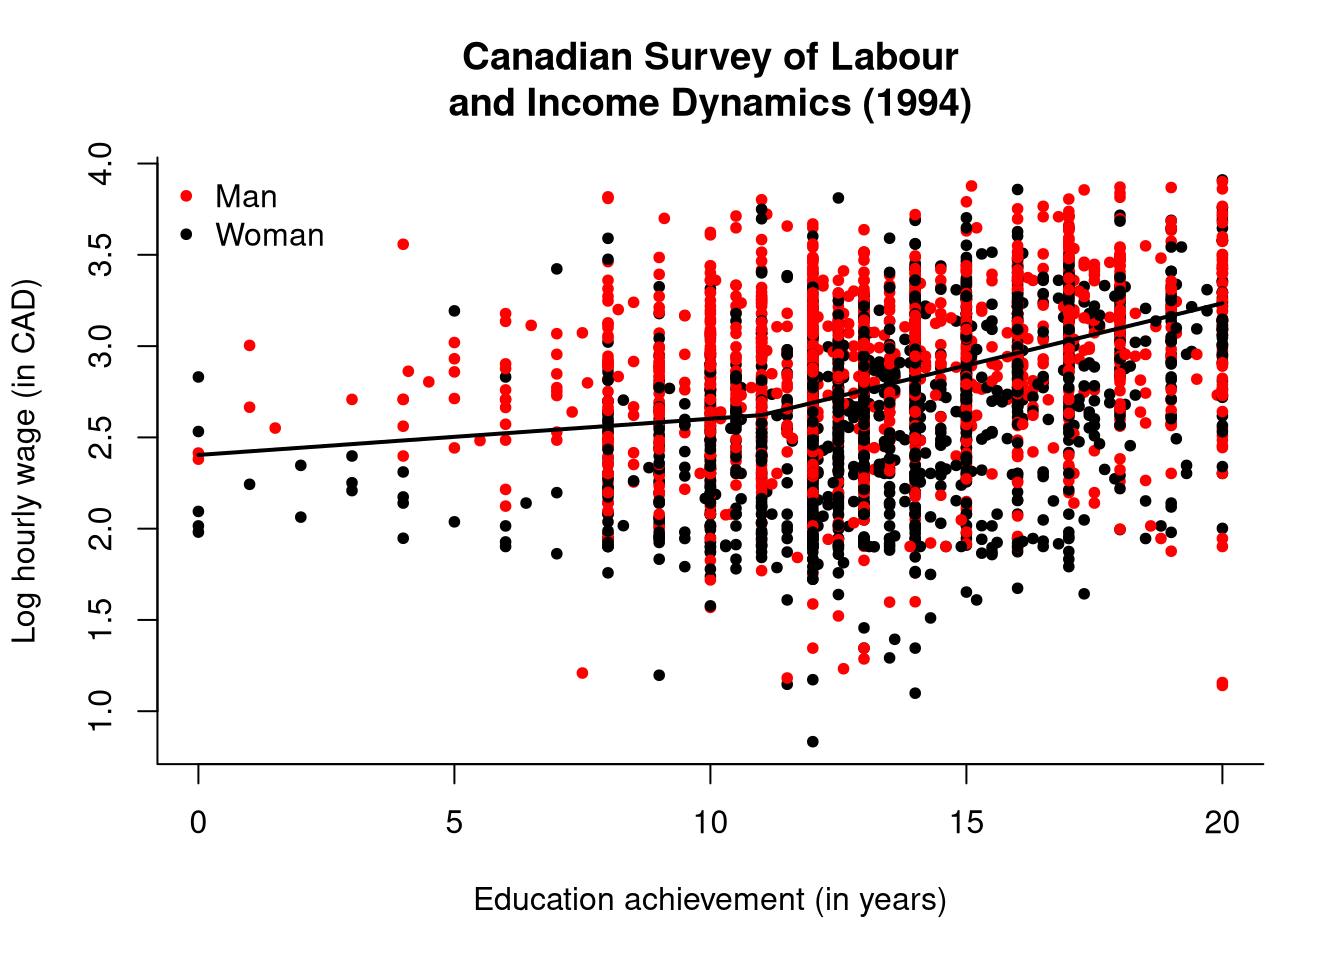
\includegraphics[width=0.7\linewidth]{LineaRModels_files/figure-latex/ex5.3-1} \end{center}

\begin{Shaded}
\begin{Highlighting}[]
\CommentTok{## Clear pattern: women are paid less for equivalent qualification}

\CommentTok{## Add gender as covariate}
\NormalTok{educ_lm <-}\StringTok{ }\KeywordTok{lm}\NormalTok{(lhwages }\OperatorTok{~}\StringTok{ }\NormalTok{., }\DataTypeTok{data=}\NormalTok{ labour) }
\CommentTok{# fit lm with all columns but lhwages}
\CommentTok{## or equivalently}
\CommentTok{#update(educ_lm, . ~ . + gender)}
\KeywordTok{summary}\NormalTok{(educ_lm)}
\end{Highlighting}
\end{Shaded}

\begin{verbatim}
## 
## Call:
## lm(formula = lhwages ~ ., data = labour)
## 
## Residuals:
##      Min       1Q   Median       3Q      Max 
## -2.10953 -0.25249  0.02989  0.28176  1.27908 
## 
## Coefficients:
##             Estimate Std. Error t value     Pr(>|t|)
## (Intercept) 2.200103   0.055375  39.731      < 2e-16
## education   0.026589   0.004673   5.690 0.0000000138
## genderMale  0.256471   0.014771  17.363      < 2e-16
## pseduc      0.037459   0.007322   5.116 0.0000003308
## 
## Residual standard error: 0.4154 on 3183 degrees of freedom
## Multiple R-squared:  0.1897, Adjusted R-squared:  0.1889 
## F-statistic: 248.3 on 3 and 3183 DF,  p-value: < 2.2e-16
\end{verbatim}

\begin{Shaded}
\begin{Highlighting}[]
\KeywordTok{confint}\NormalTok{(educ_lm)}
\end{Highlighting}
\end{Shaded}

\begin{verbatim}
##                  2.5 %     97.5 %
## (Intercept) 2.09152815 2.30867726
## education   0.01742684 0.03575089
## genderMale  0.22750913 0.28543379
## pseduc      0.02310256 0.05181598
\end{verbatim}

\begin{Shaded}
\begin{Highlighting}[]
\KeywordTok{detach}\NormalTok{(labour)}
\end{Highlighting}
\end{Shaded}

The coefficient for gender is still statistically significative at level \(\alpha=5\%\) after adjusting for the education level.

\hypertarget{analysis-of-variance}{%
\chapter{Analysis of variance}\label{analysis-of-variance}}

Consider the linear model \(\boldsymbol{Y} = \mathbf{1}_n\alpha + \mathbf{Z}\boldsymbol{\beta} + \boldsymbol{\varepsilon}\)
where \(\mathbf{X}=(\mathbf{1}_n^\top, \mathbf{Z}^\top)^\top\) is a full rank \(n \times p\) design matrix.
Let as usual \(\mathrm{TSS} = \boldsymbol{y}^\top\mathbf{M}_{\mathbf{1}_n}\boldsymbol{y}\), the total sum of square, and \(\mathrm{RSS}= \boldsymbol{y}^\top\mathbf{M}_{\mathbf{X}}\boldsymbol{y}\), the sum of squared residuals.
Under the assumptions of the Gaussian linear model (or asymptotically), the \(F\)-test statistic for testing the null hypothesis \(\mathrm{H}_0: \boldsymbol{\beta}=\mathbf{0}_{p-1}\) against the alternative \(\mathrm{H}_a: \boldsymbol{\beta} \in \mathbb{R}^{p-1}\) assuming the larger model is correctly specified is
\[F = \frac{(\mathrm{TSS}-\mathrm{RSS})/(p-1)}{\mathrm{RSS}/(n-p)}.\]
Under the null hypothesis, \(F \sim \mathcal{F}(p-1, n-p)\).

An ANOVA table (\texttt{anova}) arranges the information about the sum of squares decomposition, the degree of freedom and the value of the \(F\) test statistic in the following manner.

\begin{tabular}{lllll}
\toprule
Sum of squares & degrees of freedom & scaled sum of squares & test statistic & $P$-value\\
\midrule
ESS & $p-1$ & $\mathrm{ESS}/(p-1)$ & $F$ & $1-\texttt{pf}(F, p-1, n-p)$\\
RSS & $n-p$ & $\mathrm{RSS}/(n-p)$ &  & \\
\bottomrule
\end{tabular}

\hypertarget{sum-of-squares-decomposition}{%
\section{Sum of squares decomposition}\label{sum-of-squares-decomposition}}

Consider the orthogonal decomposition \[\boldsymbol{y}^\top\boldsymbol{y} = \boldsymbol{y}^\top\mathbf{M}_{\mathbf{X}}\boldsymbol{y} + \boldsymbol{y}^\top\mathbf{H}_{\mathbf{X}}\boldsymbol{y},\] along with the model \[\boldsymbol{y}  = \beta_0\mathbf{1}_n + \mathbf{X}_1\boldsymbol{\beta}_1 + \mathbf{X}_2\boldsymbol{\beta}_2 + \boldsymbol{\varepsilon}.\]

We consider four concurrent models, for \(\mathbf{X}_1\) an \(n \times p_1\) matrix and \(\mathbf{X}_2\) and \(n \times p_2\) matrix and \(\mathbf{X}_a = (\mathbf{1}_n^\top, \mathbf{X}_1^\top, \mathbf{X}_2^\top)^\top\) and \(n \times p = n \times (1+p_1+p_2)\) full rank matrix.

\begin{enumerate}
\def\labelenumi{(\alph{enumi})}
\tightlist
\item
  the full model with both predictors, \(\mathrm{M}_a: \boldsymbol{y} = \beta_0\mathbf{1}_n + \mathbf{X}_1\boldsymbol{\beta}_1 + \mathbf{X}_2\boldsymbol{\beta}_2 + \boldsymbol{\varepsilon}.\),
\item
  the restricted model with \(\mathrm{M}_b: \boldsymbol{\beta}_2=0\) and only the first predictor, of the form \(\boldsymbol{y} = \beta_0\mathbf{1}_n + \mathbf{X}_1\boldsymbol{\beta}_1 + \boldsymbol{\varepsilon}.\),
\item
  the restricted model with \(\mathrm{M}_c: \boldsymbol{\beta}_1=0\) and only the second predictor, of the form \(\boldsymbol{y} = \beta_0\mathbf{1}_n + \mathbf{X}_2\boldsymbol{\beta}_2 + \boldsymbol{\varepsilon}.\)
\item
  the intercept-only model \(\mathrm{M}_d: \boldsymbol{y} = \beta_0\mathbf{1}_n + \boldsymbol{\varepsilon}\).
\end{enumerate}

Let \(\mathbf{X}_a\), \(\mathbf{X}_b\), \(\mathbf{X}_c\), and \(\mathbf{X}_d\) be the corresponding design matrices.

\textbf{R} uses an orthogonal decomposition of the projection matrix on to \(\mathbf{X}_a\), \(\mathbf{H}_{\mathbf{X}_a}\) into two parts: \(\mathbf{H}_{\mathbf{X}_a}= \mathbf{H}_{\mathbf{X}_b} + \mathbf{H}_{\mathbf{M}_{\mathbf{X}_b}\mathbf{X}_2}.\) The last term is the contribution of \(\mathbf{X}_2\) to the model fit when \(\mathbf{1}_n, \mathbf{X}_1\) are already part of the model. We can form the sum of squares of the regression using this decomposition. We use the notation \(\mathrm{SSR}(\mathbf{H}) = \boldsymbol{y}^\top\mathbf{H}\boldsymbol{y}\) to denote the sum of squares obtained by projecting \(\boldsymbol{y}\) onto the span of \(\mathbf{H}\).

We have
\[\mathrm{SSR}(\mathbf{H}_{\mathbf{M}_{\mathbf{X}_b}\mathbf{X}_2}) = \mathrm{SSR}(\mathbf{H}_{\mathbf{X}_a}) - \mathrm{SSR}(\mathbf{H}_{\mathbf{X}_b}).\]
that is, the difference in sum of squared from the regression with model \(\mathrm{M}_a\) versus that from regression \(\mathrm{M}_b.\) This is the sum of squares from the regression that are due to the addition of \(\mathbf{X}_2\) to a model that already contains \((\mathbf{1}_n, \mathbf{X}_1)\) as regressors.

The usual \(F\)-test statistic for the null hypothesis \(\mathscr{H}_0: \boldsymbol{\beta}_2=0\) can be written as
\[F = \frac{\mathrm{SSR}(\mathbf{H}_{\mathbf{M}_{\mathbf{X}_b}\mathbf{X}_2})/p_2}{\mathrm{RSS}_a/(n-p)} = \frac{(\mathrm{RSS}_b-\mathrm{RSS}_a)/p_2}{\mathrm{RSS}_a/(n-p)} \sim \mathcal{F}(p_2, n-p).\]
The last equality follows by noting that \(\mathrm{SSR}(\mathbf{H}_{\mathbf{X}_b})+ \mathrm{RSS}_b=\mathrm{SSR}(\mathbf{H}_{\mathbf{X}_a})+ \mathrm{RSS}_a\).

\hypertarget{the-decomposition-of-squares-in-r}{%
\subsection{\texorpdfstring{The decomposition of squares in \textbf{R}}{The decomposition of squares in R}}\label{the-decomposition-of-squares-in-r}}

Let us illustrate how to obtain the various quantities presented above using the \textbf{R} outputs.

First, we look at some data. The dataset \texttt{Chirot} from the package \texttt{carData} contains information about the 1907 Romanian peasant rebellion. We model the intensity of the rebellion as a function of commercialization of agriculture and a measure of traditionalism. We start by fitting the four models \(\mathrm{M}_a, \mathrm{M}_b, \mathrm{M}_c, \mathrm{M}_d\) detailed above with the regressors \(\mathbf{X}_1 \equiv\)\texttt{commerce}, \(\mathbf{X}_2 \equiv\)\texttt{tradition} and an intercept.

\begin{Shaded}
\begin{Highlighting}[]
\CommentTok{#install.packages("carData")}
\KeywordTok{data}\NormalTok{(Chirot, }\DataTypeTok{package =} \StringTok{"carData"}\NormalTok{)}
\CommentTok{## Fit linear model with commerce and tradition as explanatory variables}
\NormalTok{mod.a <-}\StringTok{ }\KeywordTok{lm}\NormalTok{(intensity }\OperatorTok{~}\StringTok{ }\NormalTok{commerce }\OperatorTok{+}\StringTok{ }\NormalTok{tradition, }\DataTypeTok{data =}\NormalTok{ Chirot)}
\NormalTok{mod.b <-}\StringTok{ }\KeywordTok{update}\NormalTok{(mod.a, .}\OperatorTok{~}\NormalTok{. }\OperatorTok{-}\StringTok{ }\NormalTok{tradition)  }\CommentTok{#remove tradition}
\CommentTok{## mod.b is equivalent to }
\CommentTok{# mod.b <- lm(intensity ~ commerce, data = Chirot)}
\NormalTok{mod.c <-}\StringTok{ }\KeywordTok{update}\NormalTok{(mod.a, .}\OperatorTok{~}\NormalTok{. }\OperatorTok{-}\StringTok{ }\NormalTok{commerce)  }\CommentTok{#remove tradition}
\NormalTok{mod.d <-}\StringTok{ }\KeywordTok{lm}\NormalTok{(intensity }\OperatorTok{~}\StringTok{ }\DecValTok{1}\NormalTok{, }\DataTypeTok{data =}\NormalTok{ Chirot)}
\end{Highlighting}
\end{Shaded}

First, the RSS from model \(\mathrm{M}_a\) can be extracted from the table returned by \texttt{summary} under the label \texttt{Residual\ standard\ error:}. This gives \(\widehat{\sigma}\), and \(\mathrm{RSS}_d = (n-p)\widehat{\sigma}\), where \(n-p=29\) in the present setting.

\begin{Shaded}
\begin{Highlighting}[]
\NormalTok{RSS.a <-}\StringTok{ }\KeywordTok{crossprod}\NormalTok{(}\KeywordTok{resid}\NormalTok{(mod.a))}
\NormalTok{RSS.a[}\DecValTok{1}\NormalTok{,}\DecValTok{1}\NormalTok{]}
\end{Highlighting}
\end{Shaded}

\begin{verbatim}
## [1] 41.43137
\end{verbatim}

\begin{Shaded}
\begin{Highlighting}[]
\KeywordTok{all.equal}\NormalTok{(}\KeywordTok{c}\NormalTok{(RSS.a), }\KeywordTok{summary}\NormalTok{(mod.a)}\OperatorTok{$}\NormalTok{df[}\DecValTok{2}\NormalTok{] }\OperatorTok{*}\StringTok{ }\KeywordTok{summary}\NormalTok{(mod.a)}\OperatorTok{$}\NormalTok{sigma}\OperatorTok{^}\DecValTok{2}\NormalTok{)}
\end{Highlighting}
\end{Shaded}

\begin{verbatim}
## [1] TRUE
\end{verbatim}

The function \texttt{anova} outputs the following:

\begin{Shaded}
\begin{Highlighting}[]
\KeywordTok{anova}\NormalTok{(mod.a)}
\end{Highlighting}
\end{Shaded}

\begin{verbatim}
## Analysis of Variance Table
## 
## Response: intensity
##           Df Sum Sq Mean Sq F value      Pr(>F)
## commerce   1 50.066  50.066 35.0438 0.000001985
## tradition  1  6.074   6.074  4.2514     0.04828
## Residuals 29 41.431   1.429
\end{verbatim}

The function \texttt{anova} considers the \emph{sequential} decomposition
\(\mathbf{H}_{\mathbf{X}_a}=\mathbf{H}_{\mathbf{1}_n} + \mathbf{H}_{\mathbf{M}_{\mathbf{1}_n}\mathbf{X}_1} + \mathbf{H}_{\mathbf{M}_{\mathbf{X}_b}\mathbf{X}_2}\).
The column \texttt{Sum\ Sq} gives

\begin{itemize}
\tightlist
\item
  1st line: the contribution for \texttt{commerce}, \(\boldsymbol{y}^\top\mathbf{H}_{\mathbf{M}_{\mathbf{1}_n}\mathbf{X}_1}\boldsymbol{y}\),
\item
  2nd line: \(\boldsymbol{y}^\top\mathbf{H}_{\mathbf{M}_{\mathbf{X}_b}\mathbf{X}_2}\boldsymbol{y}\) and
\item
  3rd line: the residuals sum of squares \(\mathrm{RSS}_a\).
\end{itemize}

These are the conditional sum of squares from the regression for the additional variable.
The test statistics corresponding to the \(F\) and \(P\)-values in the table are
\[F_1 = \frac{\mathrm{SSR}(\mathbf{H}_{\mathbf{M}_{\mathbf{1}_n}\mathbf{X}_1})/p_1}{\mathrm{RSS}/(n-p)}\]
and
\[F_2 = \frac{\mathrm{SSR}(\mathbf{H}_{\mathbf{M}_{\mathbf{X}_b}\mathbf{X}_2})/p_2}{\mathrm{RSS}/(n-p)}.\]
Note that the residual sum of squares from the denominator is that of the full model in both cases. It is orthogonal to the numerator, but not equal to the residuals from the model \(\mathrm{M}_b\) for \(F_1\).

Recall that the order in which the variables enter the model matters when performing model selection unless your regressors are orthogonal. We thus obtain a different output if we specify instead

\begin{Shaded}
\begin{Highlighting}[]
\KeywordTok{anova}\NormalTok{(}\KeywordTok{lm}\NormalTok{(intensity }\OperatorTok{~}\StringTok{ }\NormalTok{tradition }\OperatorTok{+}\StringTok{ }\NormalTok{commerce, }\DataTypeTok{data =}\NormalTok{ Chirot))}
\end{Highlighting}
\end{Shaded}

\begin{verbatim}
## Analysis of Variance Table
## 
## Response: intensity
##           Df Sum Sq Mean Sq F value     Pr(>F)
## tradition  1 19.673  19.673  13.770   0.000872
## commerce   1 36.467  36.467  25.525 0.00002194
## Residuals 29 41.431   1.429
\end{verbatim}

The \texttt{F} and \texttt{Pr(\textgreater{}F)} columns now correspond to
\[F_1' = \frac{\mathrm{SSR}(\mathbf{H}_{\mathbf{M}_{\mathbf{1}_n}\mathbf{X}_2})/p_2}{\mathrm{RSS}/(n-p)}\]
and
\[F_2' = \frac{\mathrm{SSR}(\mathbf{H}_{\mathbf{M}_{\mathbf{X}_c}\mathbf{X}_1})/p_1}{\mathrm{RSS}/(n-p)}.\]

\hypertarget{dropping-or-adding-variables}{%
\subsection{Dropping or adding variables}\label{dropping-or-adding-variables}}

The function \texttt{drop1} allows you to test for model simplification, the hypothesis that either model (\(b\)) or model (\(c\)) is an adequate simplification of the full model (\(a\)). The output includes the RSS value in addition to the sum of squared decomposition from the previous tables. In both cases here, the null hypothesis that the simpler model with \(\beta_2=0\) or \(\beta_1=0\) (against the alternative that the model with \(\boldsymbol{\beta} \in \mathbb{R}^2\) is correct) is rejected at significance level \(\alpha = 5\%\).

\begin{Shaded}
\begin{Highlighting}[]
\KeywordTok{drop1}\NormalTok{(mod.a, }\DataTypeTok{test =} \StringTok{'F'}\NormalTok{)}
\end{Highlighting}
\end{Shaded}

\begin{verbatim}
## Single term deletions
## 
## Model:
## intensity ~ commerce + tradition
##           Df Sum of Sq    RSS    AIC F value     Pr(>F)
## <none>                 41.431 14.266                   
## commerce   1    36.467 77.898 32.469 25.5252 0.00002194
## tradition  1     6.074 47.505 16.643  4.2514    0.04828
\end{verbatim}

These \(F\) values are the same as those obtained with the call on \texttt{anova} for the full model and the output is probably less confusing.

There is a similar command to add variables, called \texttt{add1}. You can try running \texttt{add1(mod.c,\ scope\ =\ .\textasciitilde{}.\ +\ tradition,\ test\ =\ \textquotesingle{}F\textquotesingle{})} to obtain similar output to the \texttt{anova} call.

To test for a simplified model in which many of the variables are removed, we can use the general linear hypothesis framework. The function \texttt{glht} in the package \texttt{multcomp} handles this, as does the function \texttt{linearHypothesis} in \texttt{car}.

Note that in general, multiple testing leads to inflated Type-I error for the set of tests, meaning that the probability of rejecting at least one null hypothesis for \(m\) tests provided that they are all true is greater than the significance level \(\alpha\) of the individual tests. A Bonferroni correction (take \(\alpha/m\) as level if you perform \(m\) tests) could be made to alleviate this, but the power to detect will be lower.

\begin{Shaded}
\begin{Highlighting}[]
\CommentTok{#install packages `multcomp` and `car` if necessary}
\CommentTok{#Test both hypothesis separately with Bonferroni correction}
\NormalTok{jt_test <-}\StringTok{ }\NormalTok{multcomp}\OperatorTok{::}\KeywordTok{glht}\NormalTok{(mod.a, }\DataTypeTok{linfct =} \KeywordTok{rbind}\NormalTok{(}\KeywordTok{c}\NormalTok{(}\DecValTok{0}\NormalTok{, }\DecValTok{1}\NormalTok{, }\DecValTok{0}\NormalTok{), }\KeywordTok{c}\NormalTok{(}\DecValTok{0}\NormalTok{, }\DecValTok{0}\NormalTok{, }\DecValTok{1}\NormalTok{)), }
                          \DataTypeTok{test =} \KeywordTok{adjusted}\NormalTok{(}\StringTok{"bonf"}\NormalTok{))}
\KeywordTok{summary}\NormalTok{(jt_test)}
\end{Highlighting}
\end{Shaded}

\begin{verbatim}
## 
##   Simultaneous Tests for General Linear Hypotheses
## 
## Fit: lm(formula = intensity ~ commerce + tradition, data = Chirot)
## 
## Linear Hypotheses:
##        Estimate Std. Error t value  Pr(>|t|)
## 1 == 0  0.09522    0.01885   5.052 0.0000437
## 2 == 0  0.11992    0.05816   2.062    0.0911
## (Adjusted p values reported -- single-step method)
\end{verbatim}

\begin{Shaded}
\begin{Highlighting}[]
\KeywordTok{summary}\NormalTok{(jt_test, multcomp}\OperatorTok{::}\KeywordTok{Ftest}\NormalTok{())}
\end{Highlighting}
\end{Shaded}

\begin{verbatim}
## 
##   General Linear Hypotheses
## 
## Linear Hypotheses:
##        Estimate
## 1 == 0  0.09522
## 2 == 0  0.11992
## 
## Global Test:
##       F DF1 DF2      Pr(>F)
## 1 19.65   2  29 0.000004038
\end{verbatim}

\begin{Shaded}
\begin{Highlighting}[]
\CommentTok{#Test hypothesis jointly using GLHT}
\NormalTok{car}\OperatorTok{::}\KeywordTok{linearHypothesis}\NormalTok{(mod.a, }\DataTypeTok{hypothesis.matrix =} \KeywordTok{rbind}\NormalTok{(}\KeywordTok{c}\NormalTok{(}\DecValTok{0}\NormalTok{, }\DecValTok{1}\NormalTok{, }\DecValTok{0}\NormalTok{), }\KeywordTok{c}\NormalTok{(}\DecValTok{0}\NormalTok{, }\DecValTok{0}\NormalTok{, }\DecValTok{1}\NormalTok{)), }\DataTypeTok{test =} \StringTok{"F"}\NormalTok{)}
\end{Highlighting}
\end{Shaded}

\begin{verbatim}
## Linear hypothesis test
## 
## Hypothesis:
## commerce = 0
## tradition = 0
## 
## Model 1: restricted model
## Model 2: intensity ~ commerce + tradition
## 
##   Res.Df    RSS Df Sum of Sq      F      Pr(>F)
## 1     31 97.571                                
## 2     29 41.431  2     56.14 19.648 0.000004038
\end{verbatim}

You can also use the function ANOVA to test with nested model. The syntax is slightly different, but the output is exactly the same.

\begin{Shaded}
\begin{Highlighting}[]
\CommentTok{#Simpler to more complex nested models}
\KeywordTok{anova}\NormalTok{(mod.d, mod.a)}
\end{Highlighting}
\end{Shaded}

\begin{verbatim}
## Analysis of Variance Table
## 
## Model 1: intensity ~ 1
## Model 2: intensity ~ commerce + tradition
##   Res.Df    RSS Df Sum of Sq      F      Pr(>F)
## 1     31 97.571                                
## 2     29 41.431  2     56.14 19.648 0.000004038
\end{verbatim}

At this point, it is important to note that we will get different test statistics (due to different denominator) if we consider the residuals sum of squares (RSS) from the full model or the simplified model in the \(F\)-test. The test is sensitive to model misspecification and we must make sure the residual sum of squares in the denominator is at least consistent.

\hypertarget{biased-rss}{%
\subsection{Biased estimators of the residual sum of square}\label{biased-rss}}

There are two possible scenarios:

\begin{enumerate}
\def\labelenumi{\arabic{enumi}.}
\tightlist
\item
  Underfitting: you omit a variable that should be present in the model (misspecified model).
\end{enumerate}

Omitting relevant variables undully inflates the residual sum of squares. Indeed, if the true model is \(\mathrm{M}_a\) with \(\beta_2 \neq 0\), but that we fit model \(\mathrm{M}_b\) of the form \(\boldsymbol{y} = \beta_0\mathbf{1}_n + \mathbf{X}_1\boldsymbol{\beta}_1 + \boldsymbol{\varepsilon}\), then the residuals sum of squares we obtain will be \(\mathrm{RSS}_{a} + \mathrm{SSR}( \mathbf{H}_{\mathbf{M}_{\mathbf{X}_b}\mathbf{X}_2})\). This reduces the statistical significance of the other variables in turn because the \(F\)-statistic is pulled toward zero. Since our null hypothesis is that the simpler model is adequate, our power to reject the null is smaller and we will go for much simpler models than should be used.

\begin{enumerate}
\def\labelenumi{\arabic{enumi}.}
\setcounter{enumi}{1}
\tightlist
\item
  Overfitting: suppose on the contrary that we use a bigger model \(\mathrm{M}_a\) with spurious variables (overfit) and that the true model is \(\mathrm{M}_b\). The parameter estimate \(\hat{\beta}_2\) should have expectation zero and, as a result, the additional decrease in the sum of squared residuals should be also zero for the redundant variable conditional on the rest. The estimator is still unbiased; the only difference is that we use up additional degrees of freedom in the test.
\end{enumerate}

This is best illustrated using a little simulation:

\begin{Shaded}
\begin{Highlighting}[]
\KeywordTok{set.seed}\NormalTok{(}\DecValTok{1234}\NormalTok{) }\CommentTok{#RNG sequence - makes output reproducible}
\NormalTok{x1 <-}\StringTok{ }\KeywordTok{rnorm}\NormalTok{(}\DecValTok{100}\NormalTok{)}
\NormalTok{x2 <-}\StringTok{ }\KeywordTok{rexp}\NormalTok{(}\DecValTok{100}\NormalTok{)}
\NormalTok{x3 <-}\StringTok{ }\KeywordTok{rbinom}\NormalTok{(}\DataTypeTok{n =} \DecValTok{100}\NormalTok{, }\DataTypeTok{size =} \DecValTok{100}\NormalTok{, }\DataTypeTok{p =} \FloatTok{0.2}\NormalTok{)}
\NormalTok{x4 <-}\StringTok{ }\KeywordTok{runif}\NormalTok{(}\DecValTok{100}\NormalTok{)}
\NormalTok{y <-}\StringTok{ }\NormalTok{x1 }\OperatorTok{+}\StringTok{ }\NormalTok{x2 }\OperatorTok{+}\StringTok{ }\NormalTok{x3 }\OperatorTok{+}\StringTok{ }\KeywordTok{rnorm}\NormalTok{(}\DecValTok{100}\NormalTok{, }\DataTypeTok{sd =} \DecValTok{4}\NormalTok{)}
\CommentTok{#RSS/(n-p)}
\NormalTok{a_u <-}\StringTok{ }\KeywordTok{anova}\NormalTok{(}\KeywordTok{lm}\NormalTok{(y }\OperatorTok{~}\StringTok{ }\NormalTok{x1 }\OperatorTok{+}\StringTok{ }\NormalTok{x2)) }\CommentTok{#underfit}
\NormalTok{a_c  <-}\StringTok{ }\KeywordTok{anova}\NormalTok{(}\KeywordTok{lm}\NormalTok{(y }\OperatorTok{~}\StringTok{ }\NormalTok{x1 }\OperatorTok{+}\StringTok{ }\NormalTok{x2 }\OperatorTok{+}\StringTok{ }\NormalTok{x3)) }\CommentTok{#correct}
\NormalTok{a_o <-}\StringTok{ }\KeywordTok{anova}\NormalTok{(}\KeywordTok{lm}\NormalTok{(y }\OperatorTok{~}\StringTok{ }\NormalTok{x1 }\OperatorTok{+}\StringTok{ }\NormalTok{x2 }\OperatorTok{+}\StringTok{ }\NormalTok{x3 }\OperatorTok{+}\StringTok{ }\NormalTok{x4 )) }\CommentTok{#overfit}

\KeywordTok{print}\NormalTok{(}\KeywordTok{c}\NormalTok{(}\StringTok{"Underfit"}\NormalTok{ =}\StringTok{ }\NormalTok{a_u[}\StringTok{'Residuals'}\NormalTok{,}\StringTok{'Mean Sq'}\NormalTok{], }
         \StringTok{"Correct"}\NormalTok{ =}\StringTok{ }\NormalTok{a_c[}\StringTok{'Residuals'}\NormalTok{,}\StringTok{'Mean Sq'}\NormalTok{], }
        \StringTok{"Overfit"}\NormalTok{ =}\StringTok{ }\NormalTok{a_o[}\StringTok{'Residuals'}\NormalTok{,}\StringTok{'Mean Sq'}\NormalTok{]}
\NormalTok{))}
\end{Highlighting}
\end{Shaded}

\begin{verbatim}
## Underfit  Correct  Overfit 
## 34.39788 19.77853 19.96968
\end{verbatim}

\begin{Shaded}
\begin{Highlighting}[]
\CommentTok{#What is Underfit sum of square?}
\NormalTok{(a_c[}\StringTok{'Residuals'}\NormalTok{,}\StringTok{'Sum Sq'}\NormalTok{] }\OperatorTok{+}\StringTok{ }\NormalTok{a_c[}\StringTok{'x3'}\NormalTok{,}\StringTok{'Sum Sq'}\NormalTok{])}\OperatorTok{/}\NormalTok{(a_c[}\StringTok{'Residuals'}\NormalTok{,}\StringTok{'Df'}\NormalTok{] }\OperatorTok{+}\StringTok{ }\DecValTok{1}\NormalTok{)}
\end{Highlighting}
\end{Shaded}

\begin{verbatim}
## [1] 34.39788
\end{verbatim}

If there are no interactions and you wish to compare main effects conditional on all the others main effects present in the model for each of the explanatory variables, you can use the function \texttt{Anova} from the package \texttt{car}. This is the so-called Type II Anova decomposition. You could retrieve the output directly from repeated calls to \texttt{anova}.

\hypertarget{one-way-anova}{%
\section{One-way ANOVA}\label{one-way-anova}}

A one-way ANOVA is a test for equality of means in different subpopulations. Under the assumption that the observations have a common variance and that they are normally distributed, this corresponds to a Gaussian linear model with binary indicators (factors) as explanatories.
Suppose there are \(L\) possible levels and \(n_j\) is the number of observations for group \(j=1,\ldots, L\).

The one-way ANOVA model can be written as
\[y_{i_j,j} = \alpha_j + \varepsilon_{i_j,j}, \quad  \varepsilon_{i_j,j} \stackrel{\mathrm{iid}}{\sim} \mathcal{N}(0, \sigma^2)\qquad (j = 1, \ldots, L, i_j= 1, \ldots, n_j). \]
Let \(\boldsymbol{y}_j = (y_{1,j}, \ldots, y_{n_j, j})^\top\) denote the vector of observations for the first group and similarly for \(\boldsymbol{\varepsilon_j}\); we can stack observations into a single regression with a matrix \(\mathbf{X}\) of indicators variables, viz.
\[\begin{pmatrix}\boldsymbol{y}_1 \\\boldsymbol{y}_2 \\ \vdots \\ \boldsymbol{y}_L\end{pmatrix} = \begin{pmatrix} \mathbf{1}_{n_1} & \mathbf{0}_{n_1}&\cdots & \mathbf{0}_{n_1} \\
\mathbf{0}_{n_2} & \mathbf{1}_{n_2}&\ddots & \mathbf{0}_{n_2} \\
\vdots & \ddots & \ddots & \vdots\\
\mathbf{0}_{n_L} & \mathbf{0}_{n_L}&\cdots & \mathbf{1}_{n_L} 
\end{pmatrix}\begin{pmatrix} \alpha_1 \\ \alpha_2 \\\vdots \\ \alpha_L\end{pmatrix} + \begin{pmatrix}\boldsymbol{\varepsilon}_1 \\\boldsymbol{\varepsilon}_2 \\ \vdots \\ \boldsymbol{\varepsilon}_L\end{pmatrix}. \]

In a \textbf{balanced design}, the number of observations \(m\) is the same for each of the \(L\) levels of the factor. We can then write \(\mathbf{X}^\top\mathbf{X}= m\mathbf{I}_L\) and the standard errors are the same.

To test \(\mathrm{H}_0: \alpha_1 = \cdots = \alpha_L\), we can use the usual sum of squares decomposition.
The \(F\)-statistic for this test is
\[F = \frac{(\boldsymbol{y}^\top\mathbf{M}_{\mathbf{1}_n}\boldsymbol{y} - \boldsymbol{y}^\top\mathbf{M}_{\mathbf{X}}\boldsymbol{y})/(L-1)}{
\boldsymbol{y}^\top\mathbf{M}_{\mathbf{X}}\boldsymbol{y}/(n-L)} \sim \mathcal{F}(L-1, n-L).\]
and we reject the null hypothesis \(\mu_1 = \cdots = \mu_L\) against the alternative that at least one group mean is different. One crucial assumption is that all groups have the same variance.

\hypertarget{two-way-anova-and-irrelevant-hypotheses}{%
\section{Two-way ANOVA and irrelevant hypotheses}\label{two-way-anova-and-irrelevant-hypotheses}}

A two-way analysis extends the one-way ANOVA by considering two factors \(\mathbf{D}_1\) and \(\mathbf{D}_2\) respectively taking \(L_1\) and \(L_2\) levels.
The full model with interactions is usually specified using the design matrix
\(\mathbf{X} = [\mathbf{1}_n, \mathbf{D}_{1}, \mathbf{D}_2, (\mathbf{D}_1\circ \mathbf{D}_2) ]\), so the mean model is
\begin{align*}
  \mathrm{E}(Y_{i})= \omega + \sum_{j=1}^{L_1-1} \beta_j{\mathbf 1}_{D_{i1}=j+1} + \sum_{k=1}^{L_2-1}
  \gamma_k{\mathbf 1}_{D_{i2}=k+1} + \sum_{j=1}^{L_1-1}\sum_{k=1}^{L_2-1} \nu_{jk}{\mathbf 1}_{D_{i1}=j+1}{\mathbf 1}_{D_{i2}=k+1}.
 \end{align*}
Different submodels can be specified:

\begin{enumerate}
\def\labelenumi{\roman{enumi}.}
\tightlist
\item
  the intercept-only model, \(M_1\), has 1 parameter (\(\nu_{jk}=\beta_j=\gamma_k=0, j=1, \ldots, L_1-1, k = 1, \ldots, L_2-1\))
\item
  the model \(M_2\) with only the second factor (\(\nu_{jk}=\beta_j=0, j=1, \ldots, L_1-1, k = 1, \ldots, L_2-1\)) has \(L_2\) parameters
\item
  the model \(M_3\) with only the first factor (\(\nu_{jk}=\gamma_k=0, j=1, \ldots, L_1-1, k = 1, \ldots, L_2-1\)) has \(L_1\) parameters
\item
  the additive model \(M_4\) (\(\nu_{jk}=0, j=1, \ldots, L_1-1, k = 1, \ldots, L_2-1\)), has \(L_1+L_2-1\) parameters;
\item
  the additive model \(M_5\) with the interaction term has \(L_1L_2\) parameters;
\end{enumerate}

Note that we consider interaction terms only if the corresponding main effects are included. Removing main effects or lower-order
interactions while keeping higher order terms implies that the levels of the factor are not arbitrarily labelled and
rearrangement of the factors (changing the baseline) leads to potentially different conclusion.

To see this, consider the model with design matrix
\([\mathbf{1}_n, \mathbf{D}_{1}, (\mathbf{D}_1\circ \mathbf{D}_2)]\), so
\(\gamma_k=0\) \((k = 1, \ldots, L_2-1)\).

The mean level for observations in the different groups are
\begin{align*}
\mathrm{E}(Y_i \mid D_{i1}=1, D_{i2}=k) &= \omega \\
\mathrm{E}(Y_i \mid D_{i1}=j, D_{i2}=1; j > 1) &= \omega + \beta_j \\
\mathrm{E}(Y_i \mid D_{i1}=j, D_{i2}=k; j, k > 1) &= \omega + \beta_j + \nu_{jk} \\
\end{align*}
The effect of moving from level \(D_{2}=1\) to \(D_{2}=k>1\) is zero if \(D_{1}=1\), whereas it is \(\nu_{jk}\) if \(D_{1}>1\). We therefore are treating the levels as being different and the models fitted (and the inference) will differ if we change the baseline category for the factors. This means that the latter is no longer arbitrary!
In \textbf{R} this baseline is the first factor in alphabetical order, so is essentially arbitrary. In the same way we will not consider interactions without main effects, one would not consider polynomials of degree \(k\) without including the coefficients of the lower order. For a degree two polynomial of the form \(\sum_{i=0}^k \beta_ix^i\), testing the hypothesis \(\beta_i=0\) for \(i < k\) means restricting attention to polynomials whose \(k\)th order term is zero, which is usually nonsensical. Thus, any Wald test (the \(t\) values output by \texttt{summary}) corresponding to such an hypothesis should be disregarded.

\hypertarget{solutions-4}{%
\section{Solutions}\label{solutions-4}}

\hypertarget{exercise-9.3---one-way-analysis-of-variance}{%
\subsection{Exercise 9.3 - One-way analysis of variance}\label{exercise-9.3---one-way-analysis-of-variance}}

In this example, the three groups have very different variances! We carry out the testing procedure simply to show you how it is done (this does not imply we should use it in practice).

\begin{Shaded}
\begin{Highlighting}[]
\KeywordTok{options}\NormalTok{(}\DataTypeTok{show.signif.stars =} \OtherTok{FALSE}\NormalTok{)}
\CommentTok{#http://www.stat.ufl.edu/~winner/data/meniscus.txt}
\NormalTok{meniscus <-}\StringTok{ }\KeywordTok{read.table}\NormalTok{(}\StringTok{"https://lbelzile.bitbucket.io/math341/meniscus.dat"}\NormalTok{, }\DataTypeTok{header =} \OtherTok{TRUE}\NormalTok{)}
\KeywordTok{boxplot}\NormalTok{(displacement }\OperatorTok{~}\StringTok{ }\NormalTok{method, }\DataTypeTok{data =}\NormalTok{ meniscus, }\DataTypeTok{ylab =} \StringTok{"Displacement (in mm)"}\NormalTok{)}
\end{Highlighting}
\end{Shaded}

\begin{center}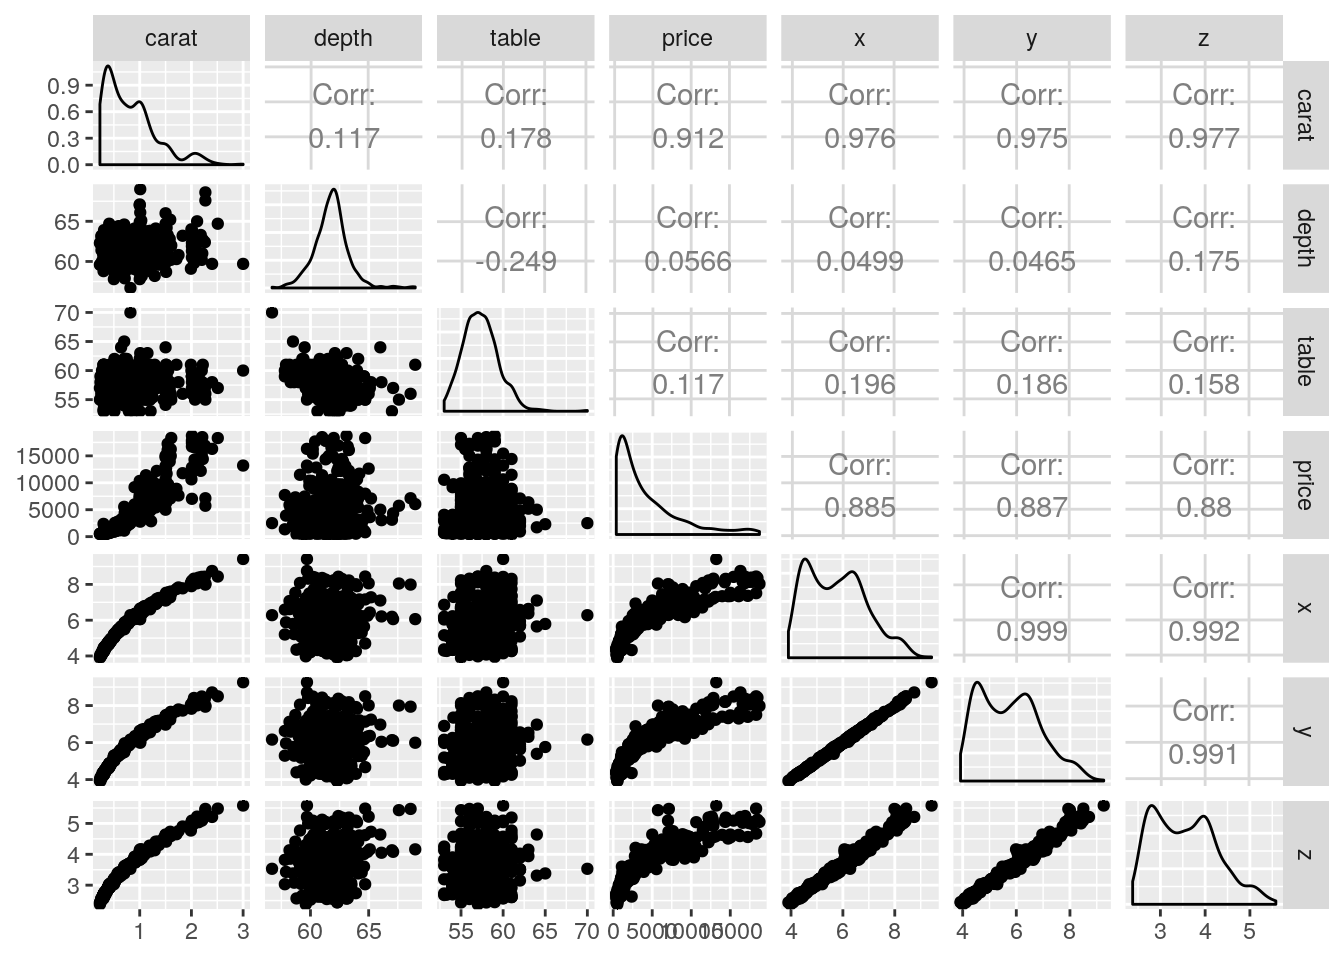
\includegraphics[width=0.7\linewidth]{LineaRModels_files/figure-latex/unnamed-chunk-42-1} \end{center}

\begin{Shaded}
\begin{Highlighting}[]
\NormalTok{lmod_men <-}\StringTok{ }\KeywordTok{lm}\NormalTok{(displacement }\OperatorTok{~}\StringTok{ }\NormalTok{method, }\DataTypeTok{data =}\NormalTok{ meniscus)}
\NormalTok{summ_men <-}\StringTok{ }\KeywordTok{summary}\NormalTok{(lmod_men)}
\CommentTok{#ANOVA table}
\NormalTok{anov_men <-}\StringTok{ }\KeywordTok{anova}\NormalTok{(lmod_men)}
\CommentTok{#F statistic with dof}
\NormalTok{summ_men}\OperatorTok{$}\NormalTok{fstatistic}
\end{Highlighting}
\end{Shaded}

\begin{verbatim}
##     value     numdf     dendf 
##  5.783689  2.000000 15.000000
\end{verbatim}

\begin{Shaded}
\begin{Highlighting}[]
\CommentTok{#P-value}
\NormalTok{anov_men[}\DecValTok{1}\NormalTok{,}\StringTok{"Pr(>F)"}\NormalTok{]}
\end{Highlighting}
\end{Shaded}

\begin{verbatim}
## [1] 0.01374261
\end{verbatim}

The \(F\) statistic for the null hypothesis \(\mu_1=\mu_2=\mu_3\) is 5.78 against the alternative that at least one group mean differ. Under the assumption of the Gaussian linear model, \(F\) follows a Fisher distribution with 2 and 15 degrees of freedom. The \(P\)-value is thus 0.01 and we therefore reject the null hypothesis that the treatment is equal at level \(\alpha = 0.05\).

The \texttt{meniscus} dat set is a balanced design, which implies that the number of observations is the same for each level of the factor. Since the entries of \(\mathbf{X}^\top\mathbf{X}\) depend on the counts for each level, they will be the same here. This implies that the standard errors are also identical for each level (except for the baseline, symbolized by the intercept). Removing the latter changes the parametrization from baseline and constrast to individual group mean.

\begin{Shaded}
\begin{Highlighting}[]
\KeywordTok{summary}\NormalTok{(lmod_men2 <-}\StringTok{ }\KeywordTok{lm}\NormalTok{(displacement }\OperatorTok{~}\StringTok{ }\DecValTok{0} \OperatorTok{+}\StringTok{ }\NormalTok{method, }\DataTypeTok{data =}\NormalTok{ meniscus))}
\end{Highlighting}
\end{Shaded}

\begin{verbatim}
## 
## Call:
## lm(formula = displacement ~ 0 + method, data = meniscus)
## 
## Residuals:
##     Min      1Q  Median      3Q     Max 
## -8.2667 -1.8500  0.2833  1.7708  5.3333 
## 
## Coefficients:
##                       Estimate Std. Error t value      Pr(>|t|)
## methodFasT-Fix          17.467      1.403  12.454 0.00000000260
## methodMeniscus Arrow    11.383      1.403   8.116 0.00000072052
## methodVertical Suture   16.950      1.403  12.085 0.00000000392
## 
## Residual standard error: 3.435 on 15 degrees of freedom
## Multiple R-squared:  0.9607, Adjusted R-squared:  0.9529 
## F-statistic: 122.3 on 3 and 15 DF,  p-value: 0.00000000009081
\end{verbatim}

\begin{Shaded}
\begin{Highlighting}[]
\KeywordTok{crossprod}\NormalTok{(}\KeywordTok{model.matrix}\NormalTok{(lmod_men2))}
\end{Highlighting}
\end{Shaded}

\begin{verbatim}
##                       methodFasT-Fix methodMeniscus Arrow
## methodFasT-Fix                     6                    0
## methodMeniscus Arrow               0                    6
## methodVertical Suture              0                    0
##                       methodVertical Suture
## methodFasT-Fix                            0
## methodMeniscus Arrow                      0
## methodVertical Suture                     6
\end{verbatim}

Note that the value of the multiple R-squared value is not the same, nor is the \(F\)-statistic. The residuals sum of square does not change because the adjustment is the same. However, without an intercept, \textbf{R} computes the decomposition
\(\boldsymbol{y}^\top\boldsymbol{y} = \mathrm{RSS} + \boldsymbol{y}^\top\mathbf{H}_{\mathbf{X}}\boldsymbol{y}\) rather than \(\mathrm{TSS} = \boldsymbol{y}^\top\mathbf{M}_{\mathbf{1}_n}\boldsymbol{y}= \mathrm{ESS}+\mathrm{RSS}\).
We have \(\mathrm{TSS} = \boldsymbol{y}^\top\boldsymbol{y}-n\bar{y}^2\).

We can compute the mean using the information on the total number of cases, since \(\bar{y} = (\hat{\mu}_1+\hat{\mu}_2 + \hat{\mu}_3)/3\).

\hypertarget{exercise-9.4---two-way-analysis-of-variance}{%
\subsection{Exercise 9.4 - Two-way analysis of variance}\label{exercise-9.4---two-way-analysis-of-variance}}

\begin{Shaded}
\begin{Highlighting}[]
\NormalTok{diet <-}\StringTok{ }\KeywordTok{read.table}\NormalTok{(}\StringTok{"https://lbelzile.bitbucket.io/math341/diet.dat"}\NormalTok{, }\DataTypeTok{header =} \OtherTok{TRUE}\NormalTok{)}
\CommentTok{#Cast strings to factors}
\NormalTok{diet}\OperatorTok{$}\NormalTok{diet.type <-}\StringTok{ }\KeywordTok{as.factor}\NormalTok{(diet}\OperatorTok{$}\NormalTok{diet.type)}
\NormalTok{diet}\OperatorTok{$}\NormalTok{gender <-}\StringTok{ }\KeywordTok{as.factor}\NormalTok{(diet}\OperatorTok{$}\NormalTok{gender)}

\CommentTok{#Check mean and variance by combination of factor}
\CommentTok{#Warning: small sample sizes}
\NormalTok{facs <-}\StringTok{ }\KeywordTok{list}\NormalTok{(diet}\OperatorTok{$}\NormalTok{diet.type, diet}\OperatorTok{$}\NormalTok{gender)}
\KeywordTok{tapply}\NormalTok{(diet}\OperatorTok{$}\NormalTok{weight.loss, facs, mean)}
\end{Highlighting}
\end{Shaded}

\begin{verbatim}
##      Female      Male
## A -3.050000 -3.650000
## B -2.607143 -4.109091
## C -5.880000 -4.233333
\end{verbatim}

\begin{Shaded}
\begin{Highlighting}[]
\KeywordTok{tapply}\NormalTok{(diet}\OperatorTok{$}\NormalTok{weight.loss, facs, var)}
\end{Highlighting}
\end{Shaded}

\begin{verbatim}
##     Female     Male
## A 4.264231 6.431667
## B 5.239176 6.376909
## C 3.570286 7.376970
\end{verbatim}

\begin{Shaded}
\begin{Highlighting}[]
\CommentTok{#Variance may not be homogeneous for men/women }
\CommentTok{#Fit model with interaction}
\NormalTok{M5 <-}\StringTok{ }\KeywordTok{lm}\NormalTok{(weight.loss }\OperatorTok{~}\StringTok{ }\NormalTok{gender }\OperatorTok{*}\StringTok{ }\NormalTok{diet.type, }\DataTypeTok{data =}\NormalTok{ diet)}
\NormalTok{M4 <-}\StringTok{ }\KeywordTok{lm}\NormalTok{(weight.loss }\OperatorTok{~}\StringTok{ }\NormalTok{gender }\OperatorTok{+}\StringTok{ }\NormalTok{diet.type, }\DataTypeTok{data =}\NormalTok{ diet)}
\NormalTok{M3 <-}\StringTok{ }\KeywordTok{lm}\NormalTok{(weight.loss }\OperatorTok{~}\StringTok{ }\NormalTok{diet.type, }\DataTypeTok{data =}\NormalTok{ diet)}
\NormalTok{M2 <-}\StringTok{ }\KeywordTok{lm}\NormalTok{(weight.loss }\OperatorTok{~}\StringTok{ }\NormalTok{gender, }\DataTypeTok{data =}\NormalTok{ diet)}
\NormalTok{M1 <-}\StringTok{ }\KeywordTok{lm}\NormalTok{(weight.loss }\OperatorTok{~}\StringTok{ }\DecValTok{1}\NormalTok{, }\DataTypeTok{data =}\NormalTok{ diet)}
\CommentTok{#ANOVA Tables (recall sequential decomposition) - prefered option}
\KeywordTok{anova}\NormalTok{(M5)}
\end{Highlighting}
\end{Shaded}

\begin{verbatim}
## Analysis of Variance Table
## 
## Response: weight.loss
##                  Df Sum Sq Mean Sq F value   Pr(>F)
## gender            1   0.28  0.2785  0.0518 0.820623
## diet.type         2  60.42 30.2086  5.6190 0.005456
## gender:diet.type  2  33.90 16.9520  3.1532 0.048842
## Residuals        70 376.33  5.3761
\end{verbatim}

\begin{Shaded}
\begin{Highlighting}[]
\CommentTok{#anova(M5) uses RSS from M5 in denominator, read table from bottom to top}
\CommentTok{#RSS values}
\NormalTok{RSS <-}\StringTok{ }\KeywordTok{anova}\NormalTok{(M1, M2, M3, M4, M5)[,}\StringTok{"RSS"}\NormalTok{]}
\CommentTok{#Backward model selection (more complex to simpler)}
\KeywordTok{drop1}\NormalTok{(M5, }\DataTypeTok{test =} \StringTok{"F"}\NormalTok{)}
\end{Highlighting}
\end{Shaded}

\begin{verbatim}
## Single term deletions
## 
## Model:
## weight.loss ~ gender * diet.type
##                  Df Sum of Sq    RSS    AIC F value  Pr(>F)
## <none>                        376.33 133.58                
## gender:diet.type  2    33.904 410.23 136.13  3.1532 0.04884
\end{verbatim}

\begin{Shaded}
\begin{Highlighting}[]
\CommentTok{#Manual calculation}
\NormalTok{F45 <-}\StringTok{ }\NormalTok{((RSS[}\DecValTok{4}\NormalTok{]}\OperatorTok{-}\NormalTok{RSS[}\DecValTok{5}\NormalTok{])}\OperatorTok{/}\DecValTok{2}\NormalTok{)}\OperatorTok{/}\NormalTok{(RSS[}\DecValTok{5}\NormalTok{]}\OperatorTok{/}\NormalTok{M5}\OperatorTok{$}\NormalTok{df.residual)}
\end{Highlighting}
\end{Shaded}

For forward model selection, we select the covariate that is the most correlated with the response first. The residual sum of square of the denominator must be correct, so we could use that of the most complex model here.

\begin{Shaded}
\begin{Highlighting}[]
\KeywordTok{anova}\NormalTok{(}\KeywordTok{lm}\NormalTok{(weight.loss }\OperatorTok{~}\StringTok{ }\NormalTok{gender }\OperatorTok{*}\StringTok{ }\NormalTok{diet.type, }\DataTypeTok{data =}\NormalTok{ diet))[}\StringTok{"gender"}\NormalTok{, }\KeywordTok{c}\NormalTok{(}\StringTok{"F value"}\NormalTok{,}\StringTok{"Pr(>F)"}\NormalTok{)] }
\end{Highlighting}
\end{Shaded}

\begin{verbatim}
##        F value Pr(>F)
## gender  0.0518 0.8206
\end{verbatim}

\begin{Shaded}
\begin{Highlighting}[]
\CommentTok{#gender is not significant}
\KeywordTok{anova}\NormalTok{(}\KeywordTok{lm}\NormalTok{(weight.loss }\OperatorTok{~}\StringTok{ }\NormalTok{diet.type }\OperatorTok{*}\StringTok{ }\NormalTok{gender, }\DataTypeTok{data =}\NormalTok{ diet))[}\StringTok{"diet.type"}\NormalTok{, }\KeywordTok{c}\NormalTok{(}\StringTok{"F value"}\NormalTok{,}\StringTok{"Pr(>F)"}\NormalTok{)] }
\end{Highlighting}
\end{Shaded}

\begin{verbatim}
##           F value   Pr(>F)
## diet.type  5.6292 0.005408
\end{verbatim}

\begin{Shaded}
\begin{Highlighting}[]
\CommentTok{#diet type is significant}

\CommentTok{#Alternatively - assume that the model is CORRECT}
\CommentTok{## Clearly not the case}
\KeywordTok{add1}\NormalTok{(M1, }\DataTypeTok{scope =} \KeywordTok{c}\NormalTok{(}\StringTok{"diet.type"}\NormalTok{,}\StringTok{"gender"}\NormalTok{), }\DataTypeTok{test =} \StringTok{"F"}\NormalTok{)}
\end{Highlighting}
\end{Shaded}

\begin{verbatim}
## Single term additions
## 
## Model:
## weight.loss ~ 1
##           Df Sum of Sq    RSS    AIC F value   Pr(>F)
## <none>                 470.93 140.62                 
## diet.type  2    60.527 410.40 134.17  5.3831 0.006596
## gender     1     0.278 470.65 142.58  0.0438 0.834827
\end{verbatim}

\begin{Shaded}
\begin{Highlighting}[]
\CommentTok{#manually computing F-test between diet.type + intercept and intercept only}
\KeywordTok{isTRUE}\NormalTok{(}\KeywordTok{all.equal}\NormalTok{( }
\NormalTok{  ((RSS[}\DecValTok{1}\NormalTok{]}\OperatorTok{-}\NormalTok{RSS[}\DecValTok{3}\NormalTok{])}\OperatorTok{/}\DecValTok{2}\NormalTok{)}\OperatorTok{/}\NormalTok{(RSS[}\DecValTok{3}\NormalTok{]}\OperatorTok{/}\NormalTok{(}\DecValTok{73}\NormalTok{)), }
  \KeywordTok{add1}\NormalTok{(M1, }\DataTypeTok{scope =} \KeywordTok{c}\NormalTok{(}\StringTok{"diet.type"}\NormalTok{,}\StringTok{"gender"}\NormalTok{), }\DataTypeTok{test =} \StringTok{"F"}\NormalTok{)[}\StringTok{"diet.type"}\NormalTok{, }\StringTok{"F value"}\NormalTok{]))}
\end{Highlighting}
\end{Shaded}

\begin{verbatim}
## [1] TRUE
\end{verbatim}

\begin{Shaded}
\begin{Highlighting}[]
\CommentTok{#Note that in the above, the RSS is that of the more complex model, but not the full model}
\KeywordTok{add1}\NormalTok{(M3, }\DataTypeTok{scope =} \StringTok{"gender"}\NormalTok{, }\DataTypeTok{test =} \StringTok{"F"}\NormalTok{)}
\end{Highlighting}
\end{Shaded}

\begin{verbatim}
## Single term additions
## 
## Model:
## weight.loss ~ diet.type
##        Df Sum of Sq    RSS    AIC F value Pr(>F)
## <none>              410.40 134.17               
## gender  1    0.1687 410.23 136.13  0.0296 0.8639
\end{verbatim}

\begin{Shaded}
\begin{Highlighting}[]
\CommentTok{#No evidence against the simpler null model with only diet}
\CommentTok{#We do not test for the interaction model without main effects included!}
\end{Highlighting}
\end{Shaded}

We can use information criterion to estimate the goodness-of-fit of the model.
The Akaike's information criterion (AIC) and Schwartz' information criterion (BIC) can be obtained by use of the functions \texttt{AIC} and \texttt{BIC}, respectively.

An alternative is Mallow's \(C_p\), which requires an estimate of \(s^2\). It is customary to select \(s^2\) as the mean residual sum of squares from the most complex model, to make the comparisons fair avoid bias to due model misspecification.
The most complex model will by construction give \(C_p=p\) (so we cannot assess the goodness-of-fit of this model using this technique). Good models are those for which the value of \(C_p\) is close to \(p\).

\begin{Shaded}
\begin{Highlighting}[]
\NormalTok{p <-}\StringTok{ }\KeywordTok{unlist}\NormalTok{(}\KeywordTok{lapply}\NormalTok{(}\KeywordTok{list}\NormalTok{(M1, M2, M3, M4, M5), }
                   \DataTypeTok{FUN =} \ControlFlowTok{function}\NormalTok{(mod)\{}\KeywordTok{length}\NormalTok{(}\KeywordTok{coef}\NormalTok{(mod))\}))}
\NormalTok{Mallow_Cp <-}\StringTok{ }\NormalTok{RSS}\OperatorTok{/}\NormalTok{RSS[}\DecValTok{5}\NormalTok{]}\OperatorTok{*}\NormalTok{(}\KeywordTok{nrow}\NormalTok{(diet)}\OperatorTok{-}\NormalTok{p[}\DecValTok{5}\NormalTok{]) }\OperatorTok{-}\StringTok{ }\KeywordTok{nrow}\NormalTok{(diet) }\OperatorTok{+}\StringTok{ }\DecValTok{2} \OperatorTok{*}\StringTok{ }\NormalTok{p}
\NormalTok{Mallow_Cp}
\end{Highlighting}
\end{Shaded}

\begin{verbatim}
## [1] 13.596261 15.544461  6.337787  8.306409  6.000000
\end{verbatim}

\begin{Shaded}
\begin{Highlighting}[]
\CommentTok{#Step function for model selection using AIC/BIC}
\CommentTok{#step(M5, direction = 'backward',trace = FALSE, k = log(76))}

\CommentTok{#Alternatively, compute each AIC/BIC value}
\NormalTok{aic_val <-}\StringTok{ }\KeywordTok{AIC}\NormalTok{(M1, M2, M3, M4, M5)}
\NormalTok{bic_val <-}\StringTok{ }\KeywordTok{BIC}\NormalTok{(M1, M2, M3, M4, M5)}
\KeywordTok{which.min}\NormalTok{(aic_val}\OperatorTok{$}\NormalTok{AIC)}
\end{Highlighting}
\end{Shaded}

\begin{verbatim}
## [1] 5
\end{verbatim}

\begin{Shaded}
\begin{Highlighting}[]
\KeywordTok{which.min}\NormalTok{(bic_val}\OperatorTok{$}\NormalTok{BIC)}
\end{Highlighting}
\end{Shaded}

\begin{verbatim}
## [1] 3
\end{verbatim}

\begin{Shaded}
\begin{Highlighting}[]
\CommentTok{#Store values in table}
\NormalTok{ICvals <-}\StringTok{ }\KeywordTok{rbind}\NormalTok{(aic_val}\OperatorTok{$}\NormalTok{AIC, bic_val}\OperatorTok{$}\NormalTok{BIC)}
\KeywordTok{colnames}\NormalTok{(ICvals) <-}\StringTok{ }\KeywordTok{paste0}\NormalTok{(}\StringTok{"M"}\NormalTok{, }\KeywordTok{seq}\NormalTok{(}\DecValTok{1}\OperatorTok{:}\DecValTok{5}\NormalTok{))}
\KeywordTok{rownames}\NormalTok{(ICvals) <-}\StringTok{ }\KeywordTok{c}\NormalTok{(}\StringTok{"AIC"}\NormalTok{, }\StringTok{"BIC"}\NormalTok{)}
\CommentTok{#Create table for Markdown}
\NormalTok{knitr}\OperatorTok{::}\KeywordTok{kable}\NormalTok{(}\KeywordTok{round}\NormalTok{(ICvals,}\DecValTok{2}\NormalTok{))}
\end{Highlighting}
\end{Shaded}

\begin{tabular}{l|r|r|r|r|r}
\hline
  & M1 & M2 & M3 & M4 & M5\\
\hline
AIC & 358.30 & 360.26 & 351.85 & 353.81 & 351.26\\
\hline
BIC & 362.96 & 367.25 & 361.17 & 365.47 & 367.57\\
\hline
\end{tabular}

\begin{Shaded}
\begin{Highlighting}[]
\CommentTok{#Create table to export in LaTeX}
\NormalTok{tab <-}\StringTok{ }\NormalTok{xtable}\OperatorTok{::}\KeywordTok{xtable}\NormalTok{(}\KeywordTok{round}\NormalTok{(ICvals,}\DecValTok{1}\NormalTok{), }\DataTypeTok{caption =} \StringTok{"Two-way ANOVA, diet data"}\NormalTok{)}
\CommentTok{#print(tab, booktabs = TRUE)}
\end{Highlighting}
\end{Shaded}

\hypertarget{hypothesis-testing}{%
\chapter{Hypothesis testing}\label{hypothesis-testing}}

This is a refresher on the notions related to hypothesis testing.

\textbf{Trial analogy}: suppose you are a member of the jury for a trial where the potential culprit stands accused of murder. If you declare him guilty, the sentence will likely be death penalty. The null hypothesis is innocence: the accusee is innocent until proven guilty. You will deliver a verdict of culpability only if the evidences are overwhelming against the accusee (you do not want to send an innocent to the death row and make a wrongful conviction).

In this setting, the verdict at the end of the trial will reflect ``this innocent until proven guilty'' mindset: you can usually only conclude that there are not enough proofs to sentence the accusee of murder, not that the person is innocent. This is why we ``fail to reject the null hypothesis'', since you gave the accusee the benefit of the doubt in the first place and examined the evidence in this optic.

Test statistics are realizations of random variables, so the \textbf{size} of a test is the probability of falsely rejecting the null hypothesis,
\[\alpha = \Pr(\text{reject }\mathrm{H}_0 \mid \mathrm{H}_0 \text{ is true}).\]This is fixed beforehand: if we take \(\alpha = 0.05\), there will be 95\% of the cases we will correctly release an innocent and 5\% of the cases where we will convict him undully (due to circumstancial factors, for example).

We illustrate various concepts with the simple model \[Y_i = \beta_0 + \varepsilon_i, \qquad\varepsilon_i \stackrel{\mathrm{iid}}{\sim} \mathcal{N}(0, \sigma^2) \qquad (i=1, \ldots, n)\]

The Wald test statistic for the null hypothesis \(\mathrm{H}_0: \beta_0=0\) against the alternative \(\mathrm{H}_a: \beta_0 \neq 0\) is \(t = \hat{\beta}_0/\mathrm{se}(\hat{\beta}_0) \sim \mathcal{T}(n-p)\).
We can compare the Student distribution with the empirical distribution of \(t\)-test obtained by simulating a large number of test statistics from the model; these should match.

\begin{Shaded}
\begin{Highlighting}[]
\NormalTok{test <-}\StringTok{ }\KeywordTok{rep}\NormalTok{(}\DecValTok{0}\NormalTok{, 10000L)}
\NormalTok{n <-}\StringTok{ }\NormalTok{10L}
\CommentTok{#Simulate Normal samples, compute t-test stat}
\ControlFlowTok{for}\NormalTok{(i }\ControlFlowTok{in} \DecValTok{1}\OperatorTok{:}\KeywordTok{length}\NormalTok{(test))\{}
\NormalTok{  y <-}\StringTok{ }\KeywordTok{rnorm}\NormalTok{(n)}
\NormalTok{  test[i] <-}\StringTok{ }\KeywordTok{mean}\NormalTok{(y) }\OperatorTok{/}\StringTok{ }\NormalTok{(}\KeywordTok{sd}\NormalTok{(y)}\OperatorTok{/}\KeywordTok{sqrt}\NormalTok{(n))}
\NormalTok{\}}
\CommentTok{#Create histogram, superimpose density of T(n-1)}
\KeywordTok{hist}\NormalTok{(test, }\DataTypeTok{breaks =} \DecValTok{50}\NormalTok{, }\DataTypeTok{probability =} \OtherTok{TRUE}\NormalTok{, }
     \DataTypeTok{main =} \StringTok{"Distribution of Wald test"}\NormalTok{, }\DataTypeTok{xlab =} \StringTok{"T"}\NormalTok{,}
     \DataTypeTok{xlim =} \KeywordTok{c}\NormalTok{(}\OperatorTok{-}\DecValTok{5}\NormalTok{, }\DecValTok{5}\NormalTok{))}
\KeywordTok{curve}\NormalTok{(}\KeywordTok{dt}\NormalTok{(x, }\DataTypeTok{df =}\NormalTok{ n }\OperatorTok{-}\StringTok{ }\DecValTok{1}\NormalTok{), }\DataTypeTok{col =} \DecValTok{2}\NormalTok{, }\DataTypeTok{add =} \OtherTok{TRUE}\NormalTok{, }
      \DataTypeTok{from =} \DecValTok{-5}\NormalTok{, }\DataTypeTok{to =} \DecValTok{5}\NormalTok{)}
\end{Highlighting}
\end{Shaded}

\begin{center}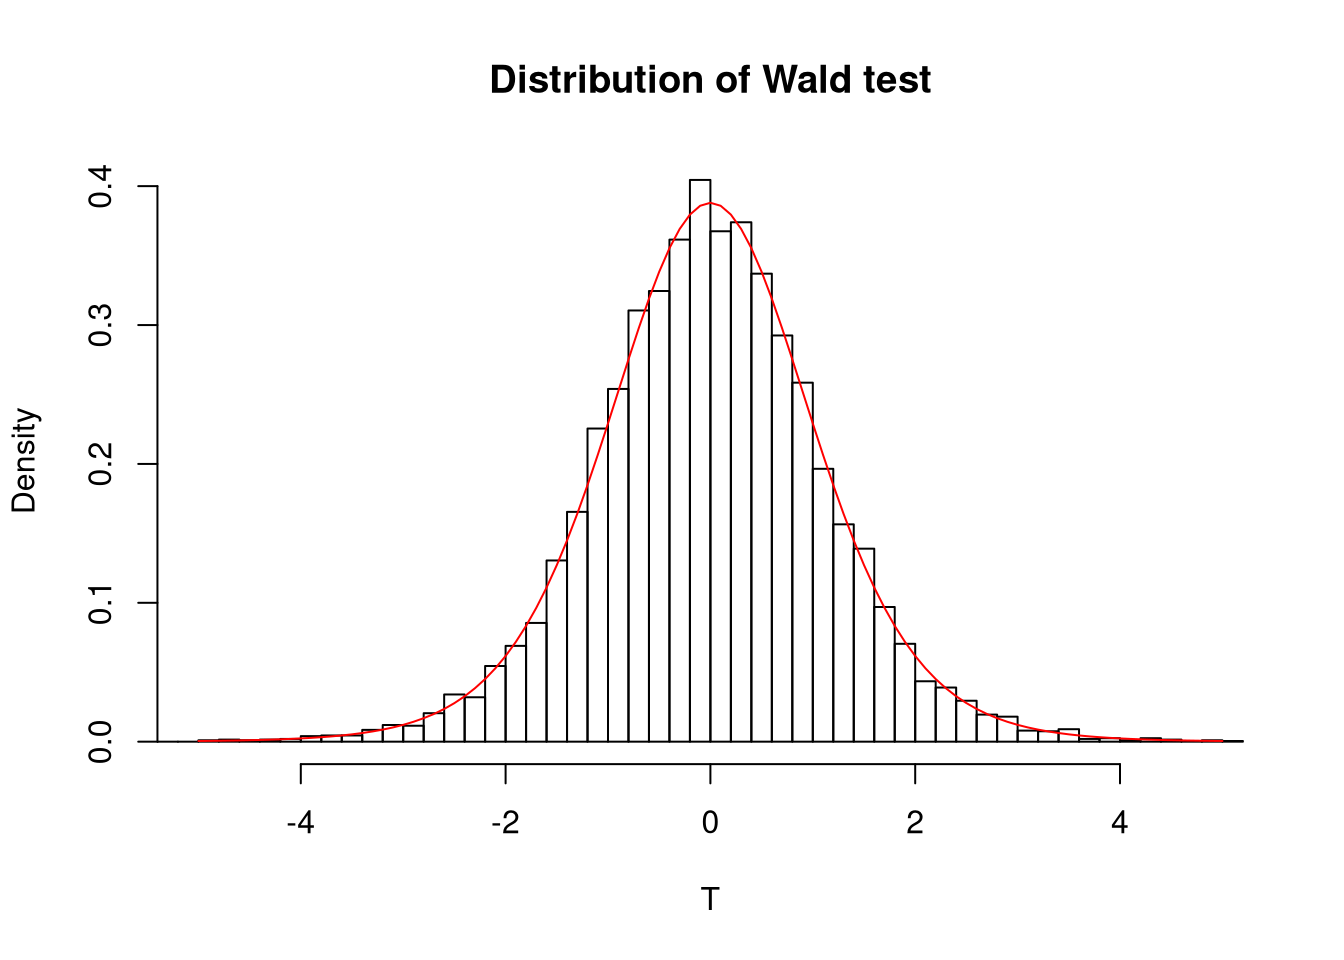
\includegraphics[width=0.7\linewidth]{LineaRModels_files/figure-latex/distrtest-1} \end{center}

If the value \(|t|\) is very large, then there are evidences that \(\beta_0 \neq 0\). In this case, the probability of observing something larger than \(|t|\) under \(T \sim \mathcal{T}(n-p)\) is \(P = 1-\Pr(-t < T < t) = 1-2 \Pr(|T| < t)\), by virtue of the symmetry of the Student distribution. This probability \(P\) is called \textbf{\(P\)-value}, the probability of observing something as extreme under the null distribution.

The \textbf{power} of a test is
\[\mathrm{power} = \Pr(\text{reject } \mathrm{H}_0 \mid \mathrm{H}_a \text{ is true}).\]
Consider the alternative \(\mathrm{H}_a: \beta = \mu \neq 0\).
For the \(t\)-test, the power is a function of \(\mu, \sigma^2\) and \(n\). Intuitively, the further \(\mu\) is from zero, the larger the chance of correctly detecting that \(\mu \neq 0\). Similarly, the more precise our mean estimate is (when \(\sigma^2\) is small), the more we have. Lastly, evidence accumulates with the sample size - here through the degrees of freedom parameter.

Even if we don't know the distribution of the test statistic under the alternative, we can simulate the power curve as a function of \(\mu, \sigma\) and \(n\).

\begin{Shaded}
\begin{Highlighting}[]
\NormalTok{n <-}\StringTok{ }\NormalTok{10L}
\NormalTok{nrep <-}\StringTok{ }\NormalTok{10000L}
\NormalTok{mu <-}\StringTok{ }\KeywordTok{seq}\NormalTok{(}\DecValTok{0}\NormalTok{, }\DecValTok{2}\NormalTok{, }\DataTypeTok{length =} \DecValTok{101}\NormalTok{)}
\NormalTok{store <-}\StringTok{ }\KeywordTok{matrix}\NormalTok{(}\DecValTok{0}\NormalTok{, }\DataTypeTok{nrow =} \KeywordTok{length}\NormalTok{(mu), }\DataTypeTok{ncol =}\NormalTok{ nrep)}
\ControlFlowTok{for}\NormalTok{(i }\ControlFlowTok{in} \DecValTok{1}\OperatorTok{:}\KeywordTok{length}\NormalTok{(mu))\{}
  \ControlFlowTok{for}\NormalTok{(j }\ControlFlowTok{in} \DecValTok{1}\OperatorTok{:}\NormalTok{nrep)\{}
    \CommentTok{# Simulate y = mu + eps, eps ~ N(0,1)}
\NormalTok{    y <-}\StringTok{ }\KeywordTok{rnorm}\NormalTok{(n, }\DataTypeTok{mean =}\NormalTok{ mu[i])}
\NormalTok{    tstat <-}\StringTok{ }\KeywordTok{mean}\NormalTok{(y) }\OperatorTok{/}\StringTok{ }\NormalTok{(}\KeywordTok{sd}\NormalTok{(y)}\OperatorTok{/}\KeywordTok{sqrt}\NormalTok{(n))}
    \CommentTok{# Compute P-value, i.e., probability Pr(|T| > t)}
\NormalTok{    pval <-}\StringTok{ }\DecValTok{2}\OperatorTok{*}\NormalTok{(}\DecValTok{1} \OperatorTok{-}\StringTok{ }\KeywordTok{pt}\NormalTok{(}\KeywordTok{abs}\NormalTok{(tstat), }\DataTypeTok{df =}\NormalTok{ n }\OperatorTok{-}\StringTok{ }\DecValTok{1}\NormalTok{))}
\NormalTok{    store[i, j] <-}\StringTok{ }\NormalTok{pval}
\NormalTok{  \}}
\NormalTok{\}}
\CommentTok{# Compute the proportion of time where p-value is below zero.}
\KeywordTok{plot}\NormalTok{(mu, }\KeywordTok{rowSums}\NormalTok{(store }\OperatorTok{<}\StringTok{ }\FloatTok{0.05}\NormalTok{)}\OperatorTok{/}\NormalTok{nrep,}
     \DataTypeTok{type =} \StringTok{"l"}\NormalTok{, }\DataTypeTok{xlab =} \KeywordTok{expression}\NormalTok{(mu), }
     \DataTypeTok{ylab =} \StringTok{"Empirical power"}\NormalTok{, }\DataTypeTok{bty =} \StringTok{"l"}\NormalTok{,}
     \DataTypeTok{main =} \KeywordTok{expression}\NormalTok{(}\KeywordTok{paste}\NormalTok{(}\StringTok{"Power curve, "}\NormalTok{, alpha, }\StringTok{"=0.05"}\NormalTok{)))}
\CommentTok{#size of test}
\KeywordTok{abline}\NormalTok{(}\DataTypeTok{h =} \FloatTok{0.05}\NormalTok{, }\DataTypeTok{lty =} \DecValTok{2}\NormalTok{)}
\CommentTok{#theoretical power - derivation follows }
\NormalTok{tquant <-}\StringTok{ }\KeywordTok{qt}\NormalTok{(}\FloatTok{0.975}\NormalTok{, }\DataTypeTok{df =}\NormalTok{ n }\OperatorTok{-}\StringTok{ }\DecValTok{1}\NormalTok{)}
\NormalTok{pow <-}\StringTok{ }\DecValTok{1} \OperatorTok{-}\StringTok{ }\NormalTok{(}\KeywordTok{pt}\NormalTok{(tquant }\OperatorTok{+}\StringTok{ }\NormalTok{mu}\OperatorTok{*}\KeywordTok{sqrt}\NormalTok{(n), }\DataTypeTok{df =}\NormalTok{ n }\OperatorTok{-}\StringTok{ }\DecValTok{1}\NormalTok{) }\OperatorTok{-}\StringTok{ }
\StringTok{                 }\KeywordTok{pt}\NormalTok{(}\OperatorTok{-}\NormalTok{tquant }\OperatorTok{+}\StringTok{ }\NormalTok{mu}\OperatorTok{*}\KeywordTok{sqrt}\NormalTok{(n), }\DataTypeTok{df =}\NormalTok{ n }\OperatorTok{-}\StringTok{ }\DecValTok{1}\NormalTok{))}
\KeywordTok{lines}\NormalTok{(mu, pow, }\DataTypeTok{col =} \DecValTok{2}\NormalTok{)}
\end{Highlighting}
\end{Shaded}

\begin{center}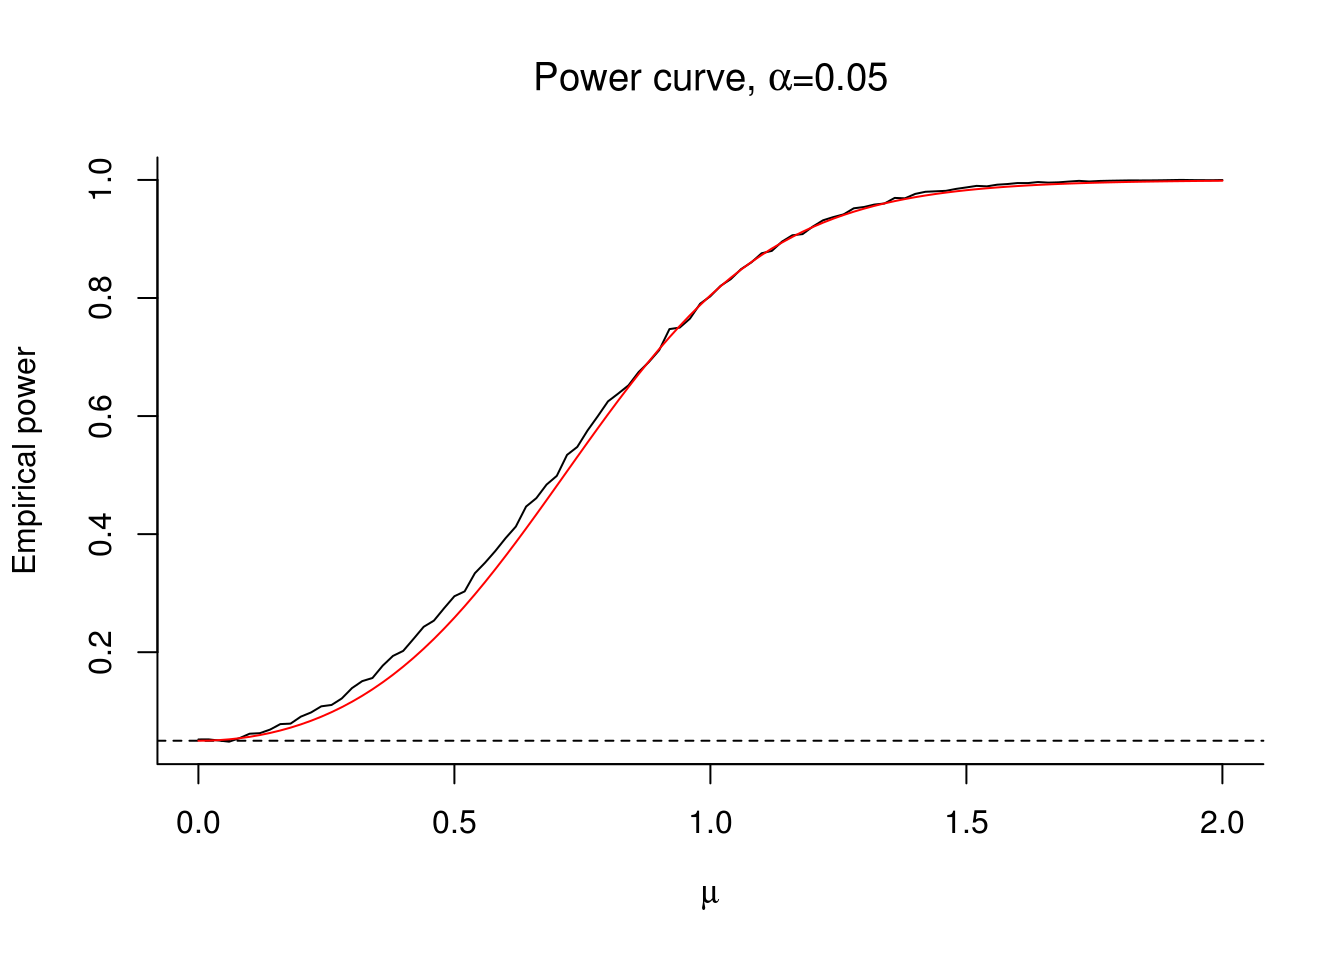
\includegraphics[width=0.7\linewidth]{LineaRModels_files/figure-latex/power-1} \end{center}

Under \(\mathrm{H}_0\), our test statistic \(T=\hat{\beta}_0/\mathrm{se}(\hat{\beta}_0)\) followed a \(\mathcal{T}(n-1)\) distribution and the cutoff value was \(\mathfrak{t}_{1-\alpha/2}\), so that under \(\mathrm{H}_0\), \(\Pr(|T| > \mathfrak{t}_{1-\alpha/2}) = \alpha\).

We can compute the power exactly as a function of \(\mu\) in this example: it is
\begin{align*}
\beta(\mu) &= 1-\Pr\left(\mathfrak{t}_{1-\alpha/2}  \leq T \leq \mathfrak{t}_{1-\alpha/2}; {\mathrm{H}_a}\right)
\\&=1-\Pr\left(\mathfrak{t}_{1-\alpha/2}  \leq \frac{\hat{\beta}_0-\mu+\mu}{\mathrm{se}(\hat{\beta}_0)} \leq \mathfrak{t}_{1-\alpha/2}; {\mathrm{H}_a}\right)
\\&=1-\Pr\left(\mathfrak{t}_{1-\alpha/2}+\frac{\mu}{\mathrm{se}(\hat{\beta}_0)}  \leq \frac{\hat{\beta}_0-\mu}{\mathrm{se}(\hat{\beta}_0)} \leq \mathfrak{t}_{1-\alpha/2}+\frac{\mu}{\mathrm{se}(\hat{\beta}_0)};{\mathrm{H}_a}\right).
\end{align*}

since now \(T^*=(\hat{\beta}_0-\mu)/\mathrm{se}(\hat{\beta}_0) \sim \mathcal{T}(n-1)\) under \(\mathrm{H}_a\). If we superimpose this curve as a function of \(\mu\), we see it matches the empirical power.

The power curve at \(\mu=0\) is 0.05, since the size of the test is \(\alpha= 0.05\) in this experiment. If we increase the size of the test, then power increases:

The probability of Type I error (falsely rejecting the null) is the size of the test, so increases with \(\alpha\). The lower the \(\alpha\), the higher the probability of Type 2 errors (not rejecting the null when the alternative is true) and the lower the power.

\begin{Shaded}
\begin{Highlighting}[]
\KeywordTok{plot}\NormalTok{(mu, pow,}
     \DataTypeTok{type =} \StringTok{"l"}\NormalTok{, }\DataTypeTok{xlab =} \KeywordTok{expression}\NormalTok{(mu), }
     \DataTypeTok{ylab =} \StringTok{"Power"}\NormalTok{, }
     \DataTypeTok{ylim =} \KeywordTok{c}\NormalTok{(}\DecValTok{0}\NormalTok{, }\DecValTok{1}\NormalTok{), }\DataTypeTok{bty =} \StringTok{"l"}\NormalTok{,}
     \DataTypeTok{main =} \StringTok{"Power curve"}\NormalTok{)}
\NormalTok{ alphav <-}\StringTok{ }\KeywordTok{c}\NormalTok{(}\FloatTok{0.05}\NormalTok{, }\FloatTok{0.001}\NormalTok{, }\FloatTok{0.01}\NormalTok{, }\FloatTok{0.1}\NormalTok{)}
\ControlFlowTok{for}\NormalTok{(alpha_ind }\ControlFlowTok{in} \DecValTok{2}\OperatorTok{:}\DecValTok{4}\NormalTok{)\{}
\NormalTok{  alpha <-}\StringTok{ }\NormalTok{alphav[alpha_ind]}
\NormalTok{  tquant <-}\StringTok{ }\KeywordTok{qt}\NormalTok{(}\DecValTok{1}\OperatorTok{-}\NormalTok{alpha}\OperatorTok{/}\DecValTok{2}\NormalTok{, }\DataTypeTok{df =}\NormalTok{ n }\OperatorTok{-}\StringTok{ }\DecValTok{1}\NormalTok{)}
\NormalTok{  pow <-}\StringTok{ }\DecValTok{1} \OperatorTok{-}\StringTok{ }\NormalTok{(}\KeywordTok{pt}\NormalTok{(tquant }\OperatorTok{+}\StringTok{ }\NormalTok{mu}\OperatorTok{*}\KeywordTok{sqrt}\NormalTok{(n), }\DataTypeTok{df =}\NormalTok{ n }\OperatorTok{-}\StringTok{ }\DecValTok{1}\NormalTok{) }\OperatorTok{-}\StringTok{ }
\StringTok{                   }\KeywordTok{pt}\NormalTok{(}\OperatorTok{-}\NormalTok{tquant }\OperatorTok{+}\StringTok{ }\NormalTok{mu}\OperatorTok{*}\KeywordTok{sqrt}\NormalTok{(n), }\DataTypeTok{df =}\NormalTok{ n }\OperatorTok{-}\StringTok{ }\DecValTok{1}\NormalTok{))}
\KeywordTok{lines}\NormalTok{(mu, pow, }\DataTypeTok{col =}\NormalTok{ alpha_ind)}
\NormalTok{\}}
\KeywordTok{legend}\NormalTok{(}\DataTypeTok{x =} \StringTok{"topleft"}\NormalTok{, }\DataTypeTok{legend =}\NormalTok{ alphav ,}\DataTypeTok{col =} \DecValTok{1}\OperatorTok{:}\DecValTok{4}\NormalTok{, }\DataTypeTok{bty =} \StringTok{"n"}\NormalTok{, }\DataTypeTok{lty =} \KeywordTok{rep}\NormalTok{(}\DecValTok{1}\NormalTok{,}\DecValTok{4}\NormalTok{))}
\end{Highlighting}
\end{Shaded}

\begin{center}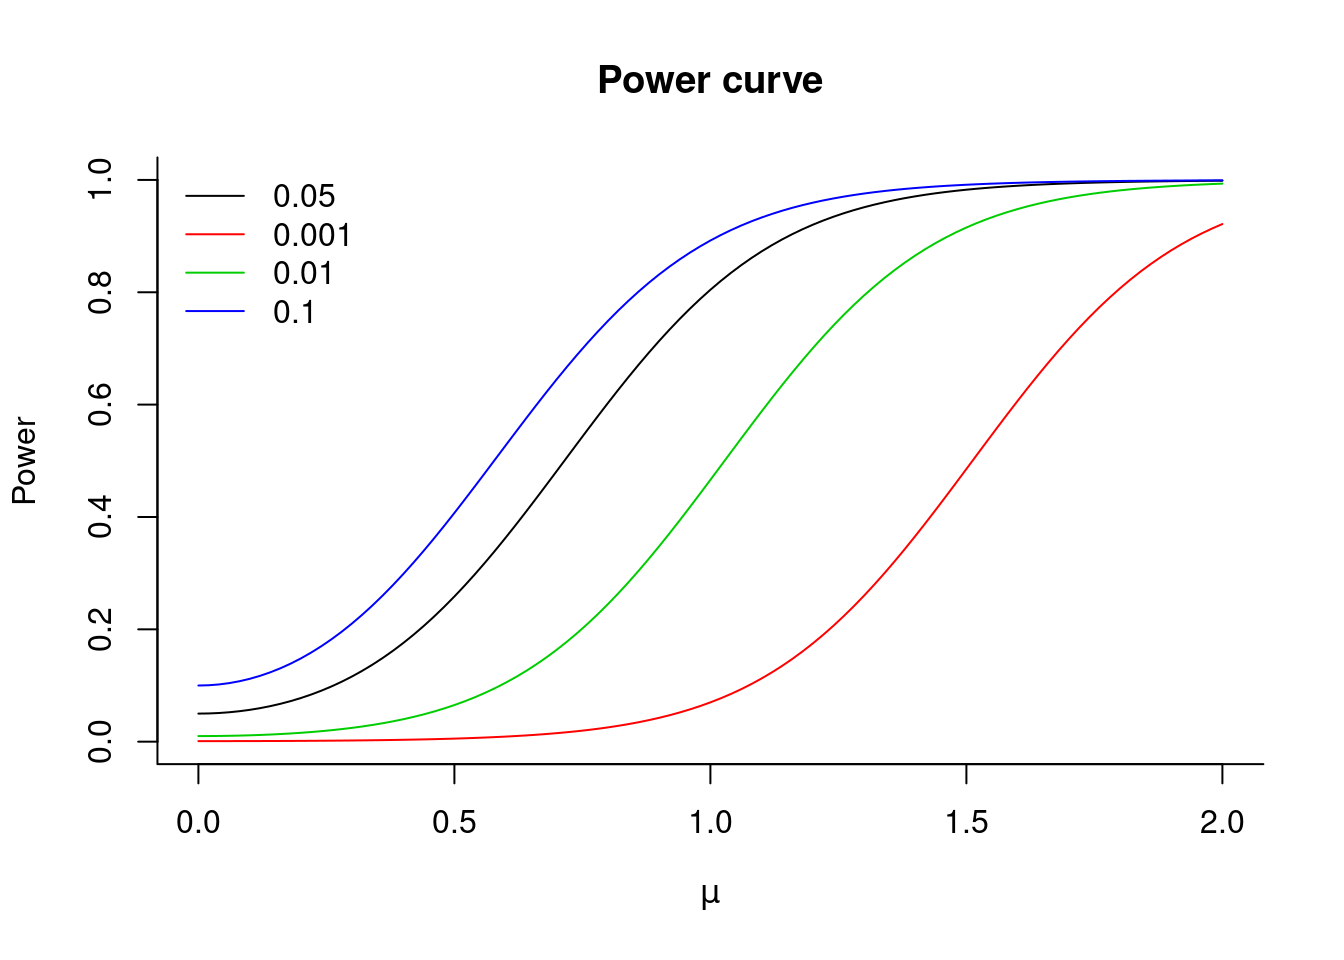
\includegraphics[width=0.7\linewidth]{LineaRModels_files/figure-latex/powermore-1} \end{center}

\hypertarget{model-selection}{%
\chapter{Model selection}\label{model-selection}}

Why perform model selection? Practitionners tend to prefer the use of a single model to model aggregation or averaging, since having a single model is easier to interpret. One guiding principle for choosing a single model is parsimony and interpretability: we want a model that is not overly complex and that does not overfit the data. This is most important if the goal of the analysis is prediction. Whenever possible, we will make comparisons between nested models.

My (personal) general strategy for model selection, given the tools covered in MATH 341, is the following:

\begin{enumerate}
\def\labelenumi{\arabic{enumi}.}
\tightlist
\item
  Start with a complex model (all additive terms, say). Look at the individual Wald tests for the marginal significance of the coefficients.
\item
  Try to simplify the full model using an \(F\) test, potentially dropping multiple terms at once. This preserves power (avoids the potential bias in the estimate of RSS in the denominator; cf.~\ref{biased-rss} and reduces the multiple testing problem that inflates Type I errors (reject the null more than \(\alpha\%\) of the time when you shouldn't).
\item
  Repeat; you can use \texttt{drop1} to further reduce the model.
\item
  Try adding interactions between variables, if any.
\item
  Compare the nested models using an information criterion such as AIC or BIC.
\item
  Select the best forward selection / backward elimination models and some additional ones (that have a nice interpretation, have low information criterion values, etc.) Compare them in terms of prediction and goodness-of-fit.
\end{enumerate}

Once you have a final model, you can interpret coefficients. Model selection \textbf{invalides} classical inference, so report coefficients and standard errors as is without overinterpreting the \(P\)-values from \texttt{summary}.

The best tool to assess the predictive power your model is the use of cross-validation. If there is no temporal structure, you can use e.g.~five-fold cross validation to find the best fitting model.

\hypertarget{example-price-of-diamonds}{%
\section{Example: Price of diamonds}\label{example-price-of-diamonds}}

This very large dataset contains the price in USD (rounded to nearest dollar) of \(n=53940\) diamonds. The explanatory variables include three ordinal factors: the quality of the \texttt{cut}, \texttt{color} and \texttt{clarity}. These are ranked from worst to best outcome. Five other variables contain the mensurements of the dimension of the diamond, rounded to the 0.01 mm. They are length \texttt{x}, width \texttt{y}, depth \texttt{z}, total depth percentage \texttt{depth} where \texttt{depth}\(=2\times z/(x + y)\), and \texttt{table}, a measure of the width of the top of the diamond. The last variable is the weight of the diamond, \texttt{carat}, rounded to the nearest 0.01.

\begin{Shaded}
\begin{Highlighting}[]
\CommentTok{#install.packages("ggplot2")}
\KeywordTok{library}\NormalTok{(ggplot2); }\KeywordTok{library}\NormalTok{(car)}
\KeywordTok{data}\NormalTok{(diamonds, }\DataTypeTok{package =} \StringTok{"ggplot2"}\NormalTok{)}
\KeywordTok{help}\NormalTok{(diamonds)}
\CommentTok{#Subsample because the dataset is very large}
\KeywordTok{set.seed}\NormalTok{(}\DecValTok{1234}\NormalTok{) }\CommentTok{#Fix RNG seed so as to make output reproducible}
\NormalTok{di <-}\StringTok{ }\NormalTok{diamonds[}\KeywordTok{sample.int}\NormalTok{(}\DataTypeTok{size =} \DecValTok{500}\NormalTok{, }\DataTypeTok{replace =} \OtherTok{FALSE}\NormalTok{, }\DataTypeTok{n =} \KeywordTok{nrow}\NormalTok{(diamonds)), ]}
\KeywordTok{attach}\NormalTok{(di)}
\end{Highlighting}
\end{Shaded}

\hypertarget{exploratory-data-analysis}{%
\subsection{Exploratory data analysis}\label{exploratory-data-analysis}}

We can look at some graphs of the data, including pair plots and some summary statistics. These are useful to spot outliers.

\begin{Shaded}
\begin{Highlighting}[]
\KeywordTok{str}\NormalTok{(di)}
\end{Highlighting}
\end{Shaded}

\begin{verbatim}
## Classes 'tbl_df', 'tbl' and 'data.frame':    500 obs. of  10 variables:
##  $ carat  : num  0.91 0.43 0.32 0.33 0.7 0.33 0.71 1.3 0.43 2.06 ...
##  $ cut    : Ord.factor w/ 5 levels "Fair"<"Good"<..: 5 4 5 5 2 5 4 2 4 5 ...
##  $ color  : Ord.factor w/ 7 levels "D"<"E"<"F"<"G"<..: 4 1 1 4 5 4 2 7 2 6 ...
##  $ clarity: Ord.factor w/ 8 levels "I1"<"SI2"<"SI1"<..: 2 3 4 2 3 7 4 4 2 4 ...
##  $ depth  : num  61.6 60.1 61.5 61.7 64.2 61.8 62.3 63.6 60.8 62.2 ...
##  $ table  : num  56 58 55 55 58 55 58 59 58 55 ...
##  $ price  : int  3985 830 808 463 1771 868 2823 5269 919 18779 ...
##  $ x      : num  6.24 4.89 4.43 4.46 5.59 4.42 5.71 6.9 4.88 8.15 ...
##  $ y      : num  6.22 4.93 4.45 4.48 5.62 4.45 5.66 6.87 4.86 8.19 ...
##  $ z      : num  3.84 2.95 2.73 2.76 3.6 2.74 3.54 4.38 2.96 5.08 ...
\end{verbatim}

\begin{Shaded}
\begin{Highlighting}[]
\KeywordTok{apply}\NormalTok{(di, }\DecValTok{2}\NormalTok{, range)}
\end{Highlighting}
\end{Shaded}

\begin{verbatim}
##      carat  cut         color clarity depth  table  price   x      y     
## [1,] "0.23" "Fair"      "D"   "I1"    "55.4" "53.0" "10076" "3.96" "3.99"
## [2,] "2.61" "Very Good" "J"   "VVS2"  "69.8" "67.0" " 9970" "8.85" "8.79"
##      z     
## [1,] "1.53"
## [2,] "5.60"
\end{verbatim}

\begin{Shaded}
\begin{Highlighting}[]
\KeywordTok{print}\NormalTok{(GGally}\OperatorTok{::}\KeywordTok{ggpairs}\NormalTok{(di[,}\OperatorTok{-}\NormalTok{(}\DecValTok{2}\OperatorTok{:}\DecValTok{4}\NormalTok{)], }\DataTypeTok{progress =} \OtherTok{FALSE}\NormalTok{))}
\end{Highlighting}
\end{Shaded}

\begin{center}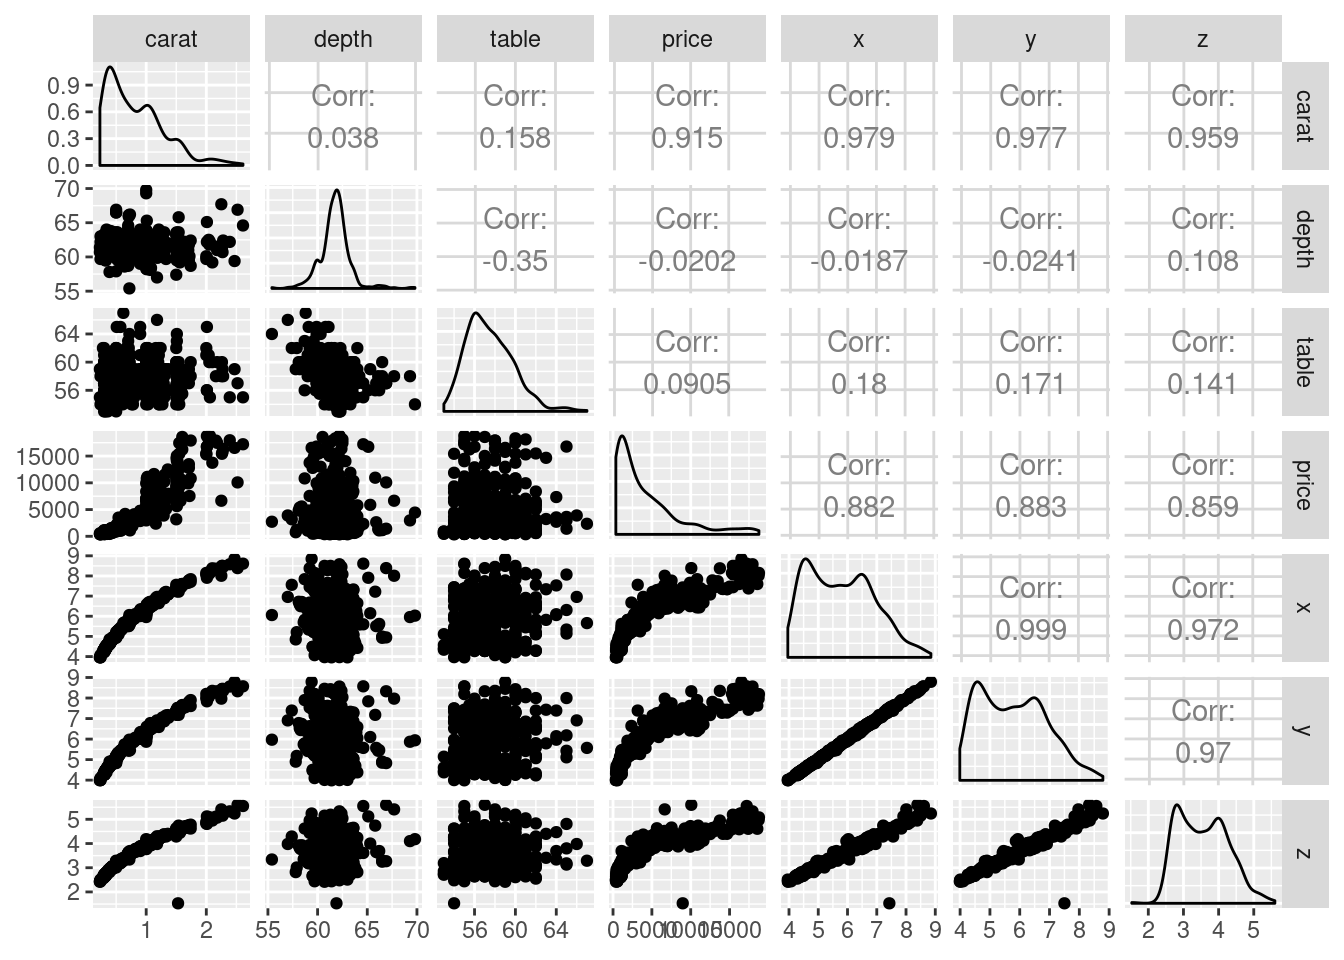
\includegraphics[width=0.7\linewidth]{LineaRModels_files/figure-latex/unnamed-chunk-47-1} \end{center}

\begin{Shaded}
\begin{Highlighting}[]
\KeywordTok{table}\NormalTok{(cut)}
\end{Highlighting}
\end{Shaded}

\begin{verbatim}
## cut
##      Fair      Good Very Good   Premium     Ideal 
##        16        46       100       123       215
\end{verbatim}

\begin{Shaded}
\begin{Highlighting}[]
\KeywordTok{table}\NormalTok{(clarity)}
\end{Highlighting}
\end{Shaded}

\begin{verbatim}
## clarity
##   I1  SI2  SI1  VS2  VS1 VVS2 VVS1   IF 
##    7   89  110  118   76   44   36   20
\end{verbatim}

\begin{Shaded}
\begin{Highlighting}[]
\KeywordTok{table}\NormalTok{(color)}
\end{Highlighting}
\end{Shaded}

\begin{verbatim}
## color
##   D   E   F   G   H   I   J 
##  57 100  77  89  95  52  30
\end{verbatim}

\begin{Shaded}
\begin{Highlighting}[]
\KeywordTok{graphics.off}\NormalTok{()}
\KeywordTok{plot}\NormalTok{(}\KeywordTok{density}\NormalTok{(carat, }\DataTypeTok{bw =} \FloatTok{0.02}\NormalTok{), }\DataTypeTok{main =} \StringTok{"Density estimate of carat"}\NormalTok{)}
\end{Highlighting}
\end{Shaded}

The most important variable is likely to be weight or width (which are strongly correlated). An explanatory data analysis reveals the relationship between \texttt{carat} and \texttt{price} to be non-linear. A logarithmic transformation of both the \texttt{price} and \texttt{carat} alleviates this and reveals the discretization of the measurements (most of the diamonds have a reported weight of 1 or 2 carats). The linear correlation between the variables \texttt{x}, \texttt{y} and \texttt{z} is close to unity (due to the regular cut of diamonds). This will potentially lead to collinearity, so the variables may not be jointly significative. There is (depending on the subset) a clearly visible outlier in \texttt{z} hat should be removed. There is no evidence of interactions between the categorical variables and the rest (not shown). Lastly, \texttt{depth} and \texttt{table} are apparently not linearly correlated with \texttt{price}.

\begin{Shaded}
\begin{Highlighting}[]
\KeywordTok{par}\NormalTok{(}\DataTypeTok{mfrow =} \KeywordTok{c}\NormalTok{(}\DecValTok{1}\NormalTok{, }\DecValTok{3}\NormalTok{), }\DataTypeTok{bty =} \StringTok{"l"}\NormalTok{)}
\KeywordTok{plot}\NormalTok{(}\DataTypeTok{x =}\NormalTok{ carat, }\DataTypeTok{y =}\NormalTok{ price, }\DataTypeTok{ylab =} \StringTok{"price (in USD)"}\NormalTok{, }\DataTypeTok{xlab =} \StringTok{"carat"}\NormalTok{)}
\KeywordTok{plot}\NormalTok{(carat, }\KeywordTok{log}\NormalTok{(price), }\DataTypeTok{ylab =} \StringTok{"log price (in USD)"}\NormalTok{, }\DataTypeTok{xlab =} \StringTok{"carat"}\NormalTok{)}
\KeywordTok{plot}\NormalTok{(carat, price, }\DataTypeTok{log=}\StringTok{"xy"}\NormalTok{, }\DataTypeTok{ylab =} \StringTok{"log price (in USD)"}\NormalTok{, }\DataTypeTok{xlab =} \StringTok{"log carat"}\NormalTok{)}
\end{Highlighting}
\end{Shaded}

\begin{center}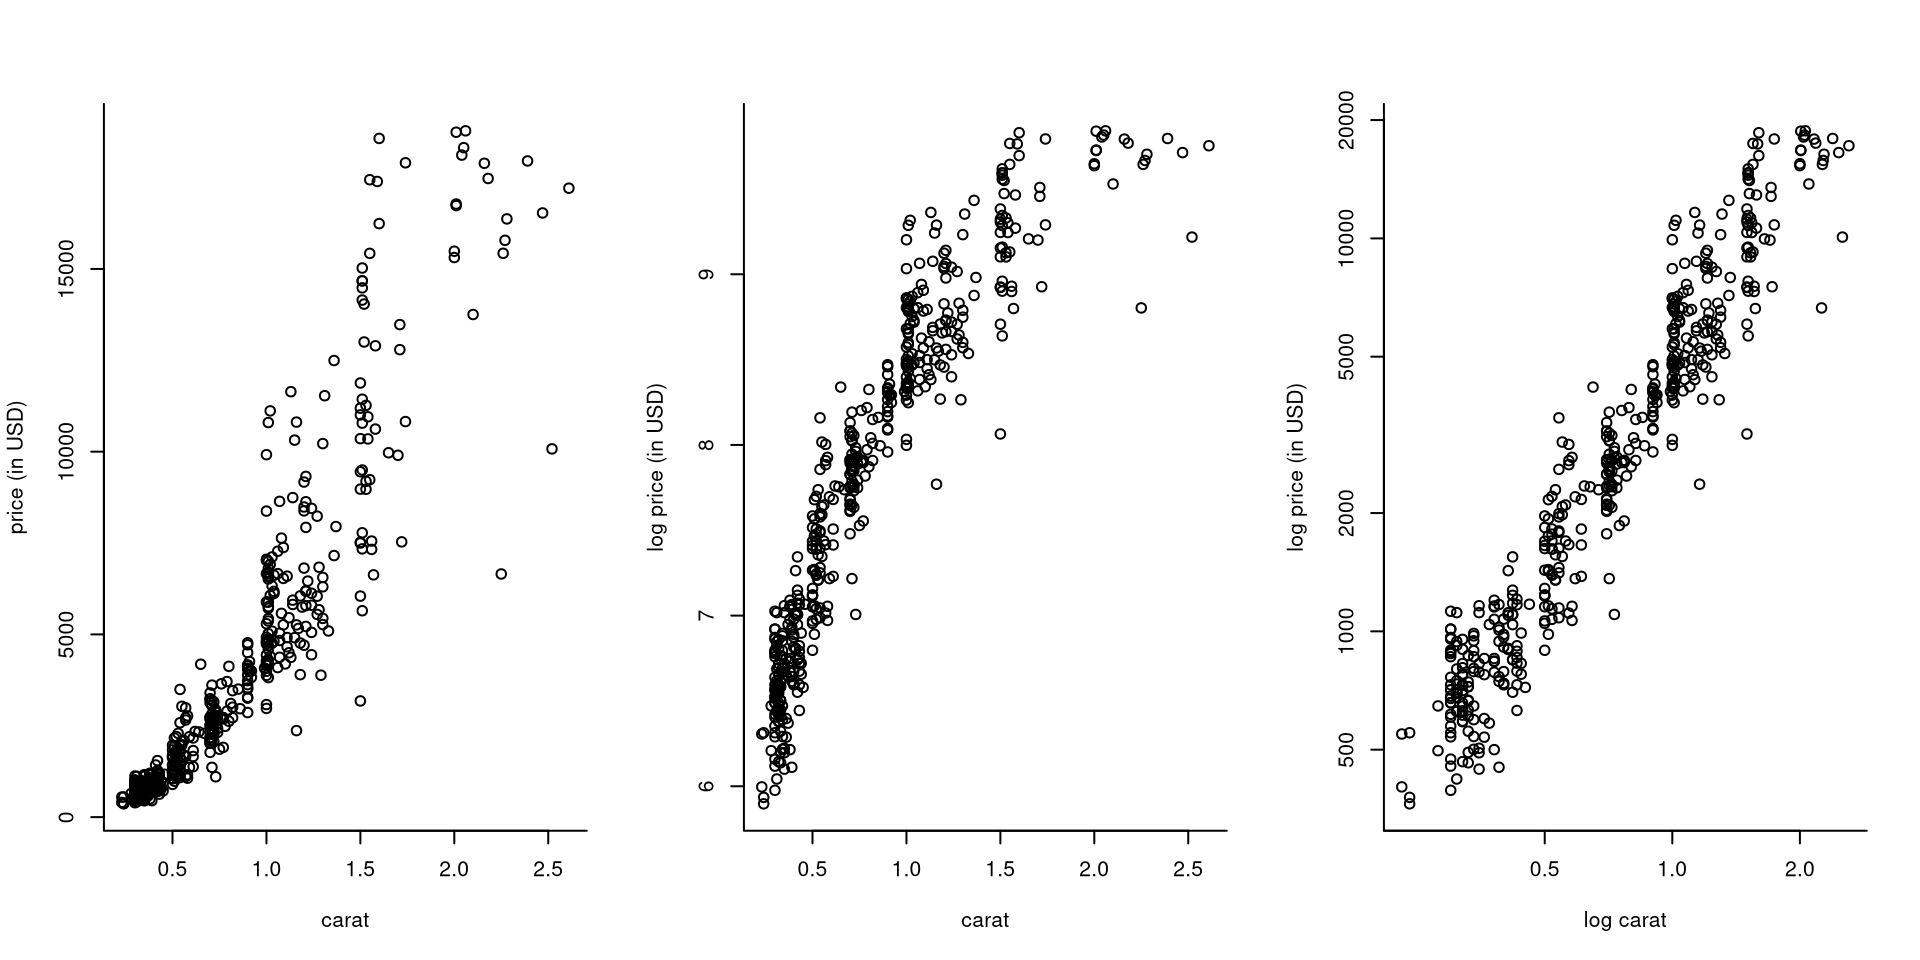
\includegraphics[width=0.7\linewidth]{LineaRModels_files/figure-latex/carat_plot-1} \end{center}

A careful explanatory data analysis with the full model reveals that, despite the fact \texttt{depth} is a transformed variable supposedly created from \texttt{x}, \texttt{y} and \texttt{z}, there are some outliers (\texttt{summary(lm(depth\ \textasciitilde{}\ -1\ +\ I(z/(x+y)),\ data\ =\ diamonds))}). The model is likely to predict poorly 1 carat and 2 carats diamonds, for which there is a lot of heterogeneity.

Sometimes, it helps to regroup the regressors to better identify patterns. This is most useful in situations where there is a lot of noise in the response (not the case here).

\begin{Shaded}
\begin{Highlighting}[]
\NormalTok{lcarat_cut <-}\StringTok{ }\KeywordTok{cut}\NormalTok{(}\KeywordTok{log}\NormalTok{(carat), }\DataTypeTok{breaks =} \KeywordTok{seq}\NormalTok{(}\OperatorTok{-}\FloatTok{1.5}\NormalTok{, }\DecValTok{1}\NormalTok{, }\DataTypeTok{by =} \FloatTok{0.25}\NormalTok{))}
\KeywordTok{boxplot}\NormalTok{(x }\OperatorTok{~}\StringTok{ }\NormalTok{lcarat_cut, }\DataTypeTok{col =} \StringTok{'grey'}\NormalTok{)}
\end{Highlighting}
\end{Shaded}

\begin{center}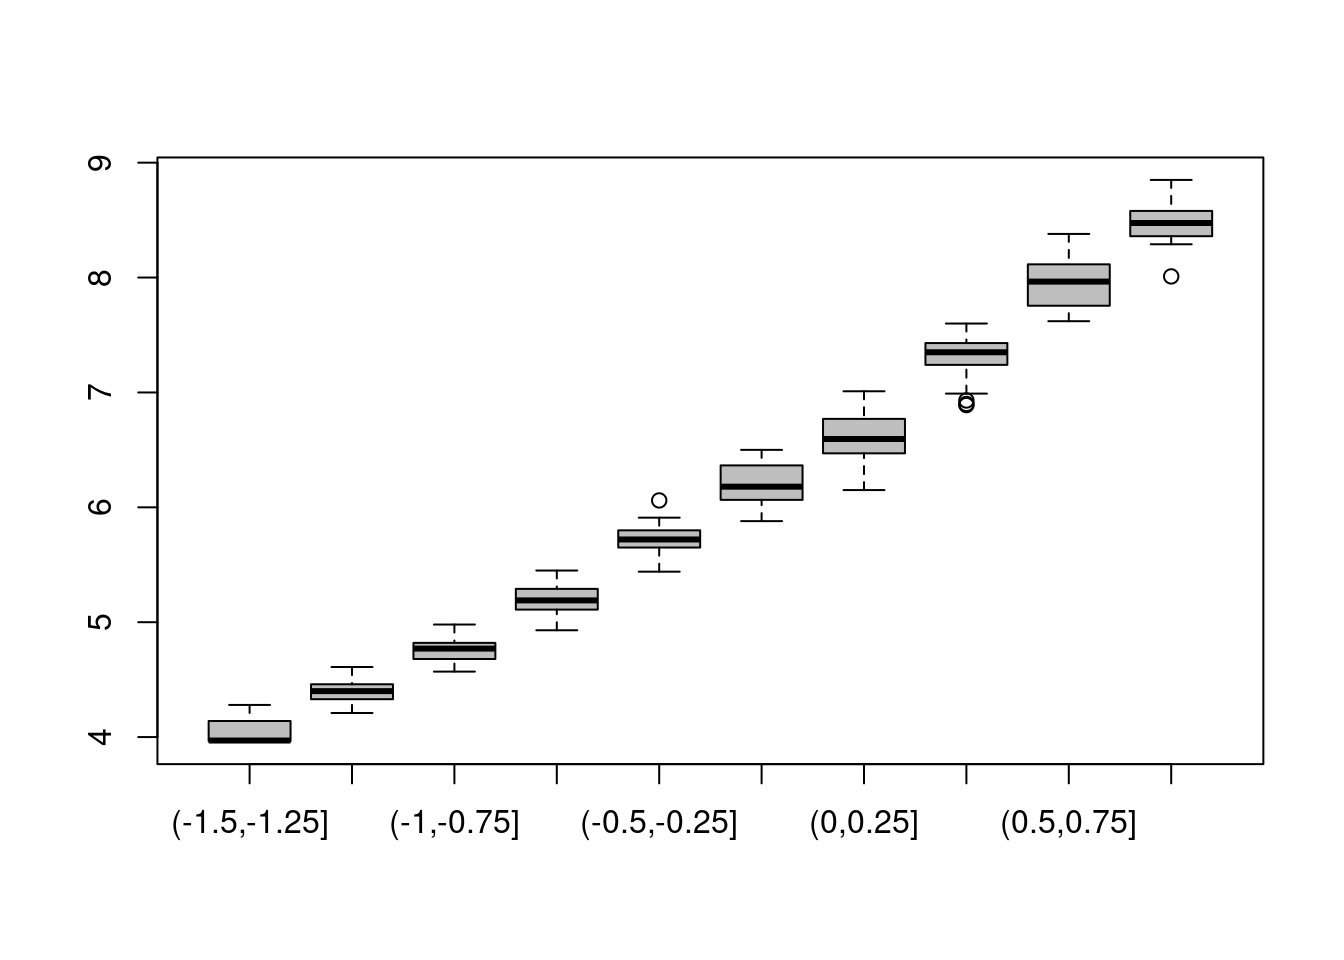
\includegraphics[width=0.7\linewidth]{LineaRModels_files/figure-latex/unnamed-chunk-48-1} \end{center}

\hypertarget{model-selection-1}{%
\subsection{Model selection}\label{model-selection-1}}

We will start with a model with all regressors but \texttt{y} and \texttt{z} (which we eliminate on grounds of multicollinearity).

\begin{Shaded}
\begin{Highlighting}[]
\CommentTok{#Small model}
\NormalTok{redu_mod <-}\StringTok{ }\KeywordTok{lm}\NormalTok{(}\KeywordTok{log}\NormalTok{(price) }\OperatorTok{~}\StringTok{ }\KeywordTok{log}\NormalTok{(carat))}
\CommentTok{#Unordered factors (so they are interpretable)}
\CommentTok{#Ordered factors use an orthogonal decomposition}
\NormalTok{cut <-}\StringTok{ }\KeywordTok{factor}\NormalTok{(cut, }\DataTypeTok{ordered =} \OtherTok{FALSE}\NormalTok{)}
\NormalTok{color <-}\StringTok{ }\KeywordTok{factor}\NormalTok{(color, }\DataTypeTok{ordered =} \OtherTok{FALSE}\NormalTok{)}
\NormalTok{clarity <-}\StringTok{ }\KeywordTok{factor}\NormalTok{(clarity, }\DataTypeTok{ordered =} \OtherTok{FALSE}\NormalTok{)}
\CommentTok{#Full additive model}
\NormalTok{full_mod <-}\StringTok{ }\KeywordTok{lm}\NormalTok{(}\KeywordTok{log}\NormalTok{(price) }\OperatorTok{~}\StringTok{ }\KeywordTok{log}\NormalTok{(carat) }\OperatorTok{+}\StringTok{ }\NormalTok{cut }\OperatorTok{+}\StringTok{ }\NormalTok{color }\OperatorTok{+}\StringTok{ }\NormalTok{clarity }\OperatorTok{+}\StringTok{ }\NormalTok{depth }\OperatorTok{+}\StringTok{ }\NormalTok{table }\OperatorTok{+}\StringTok{ }\NormalTok{x)}
\NormalTok{summ_full <-}\StringTok{ }\KeywordTok{summary}\NormalTok{(full_mod)}
\NormalTok{knitr}\OperatorTok{::}\KeywordTok{kable}\NormalTok{(}\KeywordTok{coef}\NormalTok{(summ_full), }\DataTypeTok{digits =} \DecValTok{3}\NormalTok{)}
\end{Highlighting}
\end{Shaded}

\begin{tabular}{l|r|r|r|r}
\hline
  & Estimate & Std. Error & t value & Pr(>|t|)\\
\hline
(Intercept) & 7.159 & 0.698 & 10.255 & 0.000\\
\hline
log(carat) & 1.651 & 0.101 & 16.283 & 0.000\\
\hline
cutGood & 0.118 & 0.040 & 2.964 & 0.003\\
\hline
cutVery Good & 0.114 & 0.040 & 2.878 & 0.004\\
\hline
cutPremium & 0.143 & 0.039 & 3.641 & 0.000\\
\hline
cutIdeal & 0.142 & 0.042 & 3.404 & 0.001\\
\hline
colorE & -0.056 & 0.021 & -2.604 & 0.009\\
\hline
colorF & -0.091 & 0.023 & -3.967 & 0.000\\
\hline
colorG & -0.161 & 0.022 & -7.233 & 0.000\\
\hline
colorH & -0.270 & 0.022 & -12.233 & 0.000\\
\hline
colorI & -0.400 & 0.026 & -15.568 & 0.000\\
\hline
colorJ & -0.547 & 0.030 & -18.422 & 0.000\\
\hline
claritySI2 & 0.659 & 0.053 & 12.388 & 0.000\\
\hline
claritySI1 & 0.807 & 0.053 & 15.180 & 0.000\\
\hline
clarityVS2 & 0.952 & 0.053 & 17.940 & 0.000\\
\hline
clarityVS1 & 1.035 & 0.054 & 19.192 & 0.000\\
\hline
clarityVVS2 & 1.144 & 0.056 & 20.457 & 0.000\\
\hline
clarityVVS1 & 1.224 & 0.057 & 21.461 & 0.000\\
\hline
clarityIF & 1.341 & 0.060 & 22.164 & 0.000\\
\hline
depth & 0.000 & 0.005 & 0.049 & 0.961\\
\hline
table & -0.007 & 0.004 & -1.634 & 0.103\\
\hline
x & 0.132 & 0.053 & 2.522 & 0.012\\
\hline
\end{tabular}

\begin{Shaded}
\begin{Highlighting}[]
\NormalTok{RSS_full <-}\StringTok{ }\NormalTok{summ_full}\OperatorTok{$}\NormalTok{sigma}\OperatorTok{^}\DecValTok{2} \OperatorTok{*}\StringTok{ }\NormalTok{summ_full}\OperatorTok{$}\NormalTok{df[}\DecValTok{2}\NormalTok{]}
\CommentTok{#RSS_full <- crossprod(resid(full_mod))[1]}
\end{Highlighting}
\end{Shaded}

The model fit is excellent. Unsurprisingly, all of \texttt{x}, \texttt{y} and \texttt{z} are not marginally significant if they are all included at once (output omitted), but \texttt{x} is if it is the only one included.

Recall that the \texttt{t\ value} column gives the Wald statistic \(t = \hat{\beta}_i/\mathrm{se}(\hat{\beta}_i)\), for the null hypothesis \(\beta_{i}=0\) against the two-sided alternative \(\beta_{i} \neq 0\). Under \(\mathscr{H}_0\), \(t \sim \mathcal{T}(n-p)\) and the \(P\)-value is \(2\times (1-\)\texttt{pt}\((t, n-p))\). It appears that we could get rid of \texttt{depth} and \texttt{table}, which contribute little overall. This is confirmed graphically using added-variable plots, which plots \(\mathbf{M}_{\mathbf{X}_{-j}}\boldsymbol{y}\) against \(\mathbf{M}_{\mathbf{X}_{-j}}\mathbf{x}_j\). This is the residual effect of \(\mathbf{x}_j\) after taking into account the effect of the other variables \(\mathbf{X}_{-j}\) on what remains of the response. If the variable was important, there would be a strong correlation in the variables and the slope would be non-zero. The last plots illustrates what you could see if there was residual structure (strong positive or negative correlation) or lack thereof.

\begin{Shaded}
\begin{Highlighting}[]
\KeywordTok{par}\NormalTok{(}\DataTypeTok{mfrow =} \KeywordTok{c}\NormalTok{(}\DecValTok{1}\NormalTok{, }\DecValTok{2}\NormalTok{))}
\NormalTok{car}\OperatorTok{::}\KeywordTok{avPlot}\NormalTok{(full_mod, }\DataTypeTok{variable =} \StringTok{"depth"}\NormalTok{, }\DataTypeTok{ellipse =} \OtherTok{TRUE}\NormalTok{)}
\CommentTok{#slope close to zero indicates lack of relationship}
\NormalTok{car}\OperatorTok{::}\KeywordTok{avPlot}\NormalTok{(full_mod, }\DataTypeTok{variable =} \StringTok{"log(carat)"}\NormalTok{, }\DataTypeTok{ellipse =} \OtherTok{TRUE}\NormalTok{)}
\end{Highlighting}
\end{Shaded}

\begin{center}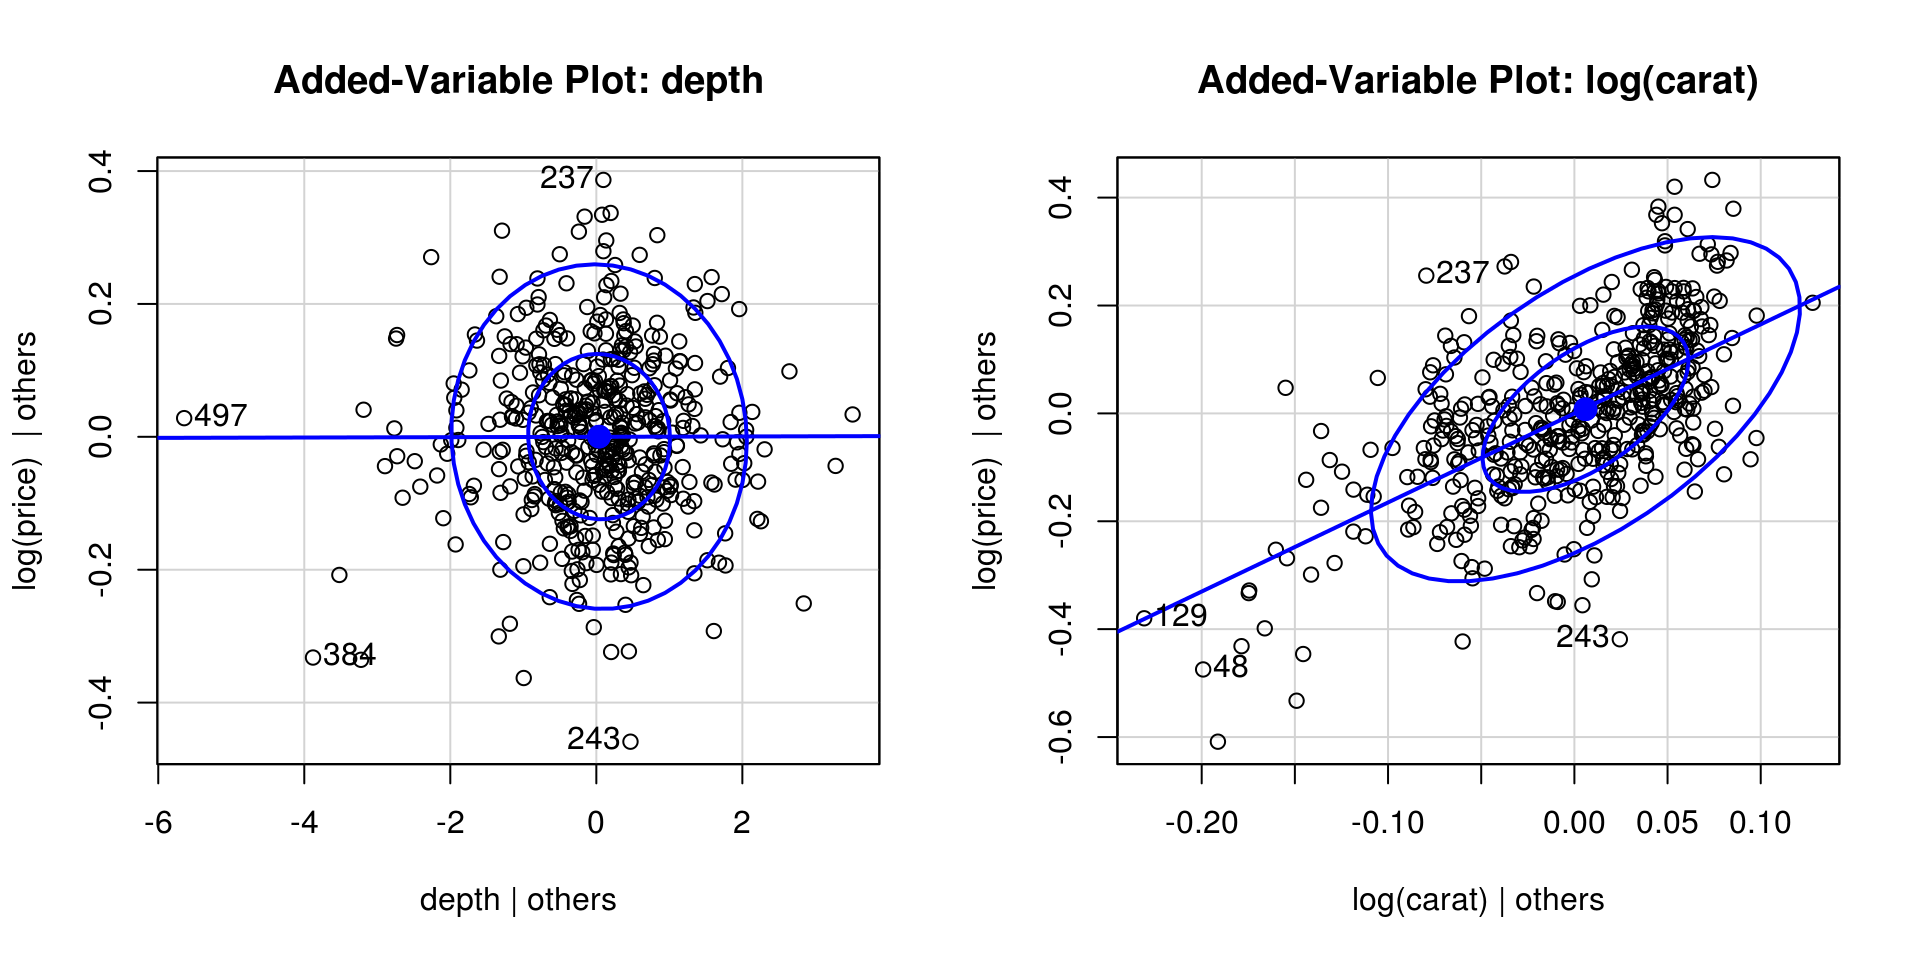
\includegraphics[width=0.7\linewidth]{LineaRModels_files/figure-latex/unnamed-chunk-49-1} \end{center}

Let us look at model simplifications.
We can obtain the \(F\) statistic for the null hypothesis \(\mathscr{H}_0: \beta_{\texttt{depth}} = \beta_{\texttt{table}}=0\) against the alternative \(\mathscr{H}_a: \{(\beta_{\texttt{depth}}, \beta_{\texttt{table}}) \in \mathbb{R}^2\}\) by running the \texttt{anova} command:

\begin{Shaded}
\begin{Highlighting}[]
\KeywordTok{anova}\NormalTok{(}\KeywordTok{lm}\NormalTok{(}\KeywordTok{log}\NormalTok{(price) }\OperatorTok{~}\StringTok{ }\KeywordTok{log}\NormalTok{(carat) }\OperatorTok{+}\StringTok{ }\NormalTok{cut }\OperatorTok{+}\StringTok{ }\NormalTok{color }\OperatorTok{+}\StringTok{ }\NormalTok{clarity }\OperatorTok{+}\StringTok{ }\NormalTok{x), full_mod)}
\end{Highlighting}
\end{Shaded}

\begin{verbatim}
## Analysis of Variance Table
## 
## Model 1: log(price) ~ log(carat) + cut + color + clarity + x
## Model 2: log(price) ~ log(carat) + cut + color + clarity + depth + table + 
##     x
##   Res.Df    RSS Df Sum of Sq      F Pr(>F)
## 1    480 7.8077                           
## 2    478 7.7503  2  0.057353 1.7686 0.1717
\end{verbatim}

The test statistic is of the form
\[F = \frac{(\mathrm{RSS}_a-\mathrm{RSS}_0)/2}{\mathrm{RSS}_0/478}\sim \mathcal{F}(2, 478)\]
and here \(F=\) 1.769; we fail to reject the null (\(P\)-value of 0.172). We have no evidence against the adequacy of the simpler model.

Since there is little difference between the reduced model RSS and that of the full additive model, we may employ either in subsequent ANOVA tests.
Let us try to drop one of the remaining variables.

\begin{Shaded}
\begin{Highlighting}[]
\KeywordTok{drop1}\NormalTok{(}\KeywordTok{lm}\NormalTok{(}\KeywordTok{log}\NormalTok{(price) }\OperatorTok{~}\StringTok{ }\KeywordTok{log}\NormalTok{(carat) }\OperatorTok{+}\StringTok{ }\NormalTok{cut }\OperatorTok{+}\StringTok{ }\NormalTok{color }\OperatorTok{+}\StringTok{ }\NormalTok{clarity }\OperatorTok{+}\StringTok{ }\NormalTok{x), }\DataTypeTok{test =} \StringTok{"F"}\NormalTok{)}
\end{Highlighting}
\end{Shaded}

\begin{verbatim}
## Single term deletions
## 
## Model:
## log(price) ~ log(carat) + cut + color + clarity + x
##            Df Sum of Sq     RSS     AIC  F value    Pr(>F)
## <none>                   7.8077 -2039.8                   
## log(carat)  1    5.7660 13.5737 -1765.2 354.4787 < 2.2e-16
## cut         4    0.4411  8.2488 -2020.3   6.7788 0.0000259
## color       6   10.1359 17.9436 -1635.7 103.8552 < 2.2e-16
## clarity     7   18.5675 26.3752 -1445.1 163.0697 < 2.2e-16
## x           1    0.0961  7.9038 -2035.6   5.9062   0.01545
\end{verbatim}

You could write the test statistics as before (with the difference in the degrees of freedom equal to the number of factor levels minus one if the variable is categorical). All the terms are statistically significant and we reject the null hypothesis of any of the tests at level \(\alpha = 5\%\). This step would mark the end of the backward elimination procedure. Note that you can (and may wish to) use the RSS from the full model \texttt{full\_mod} in the denominator of your \(F\)-tests to avoid biasing your results if retaining the null leads to a sharp decrease.

If your test statistic is small, you cannot conclude anything. This may be because the null hypothesis that the simpler model is adequate is true. It can also be due to a lack of power (you should reject, but there are not enough evidences against the null). If you proceed with the RSS from the null model, your test statistic will then be biased downward; recall section \ref{biased-rss}.

We could equally well have started with forward selection. All the variables lead to a decrease in RSS that is significant at level \(\alpha = 5\%\). We pick the most significant one and proceed.

\begin{Shaded}
\begin{Highlighting}[]
\NormalTok{add_step1 <-}\StringTok{ }\KeywordTok{add1}\NormalTok{(redu_mod, }\DataTypeTok{scope =} \KeywordTok{formula}\NormalTok{(full_mod), }\DataTypeTok{scale =}\NormalTok{ RSS_full, }\DataTypeTok{test =} \StringTok{"F"}\NormalTok{)}
\NormalTok{form <-}\StringTok{ }\KeywordTok{deparse}\NormalTok{(}\KeywordTok{formula}\NormalTok{(redu_mod))}
\ControlFlowTok{while}\NormalTok{(}\KeywordTok{length}\NormalTok{(}\KeywordTok{which}\NormalTok{(add_step1[,}\StringTok{"Pr(>F)"}\NormalTok{] }\OperatorTok{<}\StringTok{ }\FloatTok{0.05}\NormalTok{)) }\OperatorTok{>}\StringTok{ }\DecValTok{0}\NormalTok{)\{}
\NormalTok{  new_var <-}\StringTok{ }\KeywordTok{rownames}\NormalTok{(add_step1)[}\KeywordTok{which.max}\NormalTok{(add_step1[,}\StringTok{"F value"}\NormalTok{])]}
\NormalTok{  form <-}\StringTok{ }\KeywordTok{paste}\NormalTok{(form, new_var, }\DataTypeTok{sep =} \StringTok{" + "}\NormalTok{)}
\NormalTok{  add_step1 <-}\StringTok{ }\KeywordTok{add1}\NormalTok{(}\KeywordTok{update}\NormalTok{(redu_mod, }\DataTypeTok{formula =}\NormalTok{ form), }
                    \DataTypeTok{scope =} \KeywordTok{formula}\NormalTok{(full_mod), }\DataTypeTok{scale =}\NormalTok{ RSS_full, }\DataTypeTok{test =} \StringTok{"F"}\NormalTok{)}
\NormalTok{\}}
\end{Highlighting}
\end{Shaded}

The more we test using the ANOVA command, the more size distortion due to multiple testing (the type I error is inflated). A Bonferroni correction could alleviate this. Note that forward selection typically uses a biased estimate of the residual sum of square.

The variable that is the most correlated with \texttt{log(price)} is \texttt{clarity} and leads to a significant increase, so we would go for the bigger model since there is strong evidence that the model fit is better.

Both forward selection and backward elimination yielded the same model, with the three categorical variables and length. At this stage, we should try and include interactions.

\begin{Shaded}
\begin{Highlighting}[]
\KeywordTok{add1}\NormalTok{(}\KeywordTok{lm}\NormalTok{(}\DataTypeTok{formula =}\NormalTok{ form, }\DataTypeTok{data =}\NormalTok{ di),}
        \DataTypeTok{scope =}  \KeywordTok{as.formula}\NormalTok{(}\KeywordTok{paste}\NormalTok{(form, }\StringTok{"+ log(carat):color + log(carat):clarity + }
\StringTok{                                  log(carat):cut + color:cut + color:clarity + cut:clarity"}\NormalTok{, }\DataTypeTok{collapse =} \StringTok{""}\NormalTok{)),}
     \DataTypeTok{test =} \StringTok{"F"}\NormalTok{)}
\end{Highlighting}
\end{Shaded}

\begin{verbatim}
## Single term additions
## 
## Model:
## log(price) ~ log(carat) + clarity + color + x + table + cut
##                    Df Sum of Sq    RSS     AIC F value     Pr(>F)
## <none>                          7.7504 -2041.4                   
## log(carat):color    6   0.12893 7.6215 -2037.8  1.3336   0.240428
## log(carat):clarity  7   0.17840 7.5720 -2039.1  1.5886   0.136476
## log(carat):cut      4   0.39334 7.3570 -2059.5  6.3489 0.00005540
## color:cut          23   0.44771 7.3027 -2025.2  1.2155   0.225315
## clarity:color      37   1.22732 6.5231 -2053.6  2.2476 0.00006789
## clarity:cut        21   0.65138 7.0990 -2043.3  2.0012   0.005557
\end{verbatim}

The interaction between \texttt{log(carat)} and \texttt{cut} is significant at the 5\% level, idem for \texttt{clarity:color} and \texttt{clarity:cut}. Keep in mind that adding interactions leads to a large increase in the number of parameters; \texttt{clarity:color} would lead to an additional 37 parameters!

\hypertarget{information-criterion}{%
\subsection{Information criterion}\label{information-criterion}}

We have covered (old school) partial \(F\)-tests in the ANOVA section. Other widely (mis)used goodness-of-fit diagnostics are AIC and BIC. These information criterion are goodness-of-fit measures coupled with model complexity penalty. They are (under many hypothesis) estimates of the Kullback--Leibler divergence.

Akaike's An Information Criterion (AIC) is \(\mathrm{AIC}=-2\ell(\hat{\boldsymbol{\theta}}) + 2p\), while Schwartz's information criterion is \(\mathrm{BIC}=-2\ell(\hat{\boldsymbol{\theta}}) + p \log(n)\). The latter is more stringent and penalizes more heavily the complex models as more data becomes available.

Some general remarks if you use information criteria

\begin{enumerate}
\def\labelenumi{\arabic{enumi}.}
\tightlist
\item
  AIC and BIC \emph{must be} computed using maximum likelihood estimators. In a linear model, this means that the estimator of the variance is \(\hat{\sigma}^2=\mathrm{RSS}/n\) and not \(s^2\). Similarly, the ordinary least square estimator is equivalent to the MLE for \(\hat{\boldsymbol{\beta}}\) if \(\mathrm{Var}({\boldsymbol{\varepsilon}}) = \sigma^2 \mathbf{I}_n\). In \textbf{R}, you can use \texttt{BIC} and \texttt{AIC} commands on models obtained from \texttt{lm} to get those values.
\item
  Information criteria can be used to compare nested and non-nested models.
\item
  The models should include the \emph{same data} to be comparable.
\item
  If you are comparing different distributions, you need to include all the constants to make AIC values comparable.
\end{enumerate}

The function \texttt{step} allows you to do forward or backward model selection using one of the information criterion. If you use this procedure, make sure that the model returned makes sense (e.g., no interactions without main effects). You may wish to use BIC rather than AIC because the latter leads to more parsimonious models. It may be a good starting point for your model search.

\begin{Shaded}
\begin{Highlighting}[]
\NormalTok{BIC_search <-}\StringTok{ }\KeywordTok{formula}\NormalTok{(}\KeywordTok{step}\NormalTok{(full_mod, }\DataTypeTok{trace =} \DecValTok{0}\NormalTok{, }\DataTypeTok{k =} \KeywordTok{log}\NormalTok{(}\KeywordTok{nrow}\NormalTok{(di)))) }\CommentTok{#BIC}
\CommentTok{#Search within space of main effect-only models}
\NormalTok{BIC_mod <-}\StringTok{ }\KeywordTok{lm}\NormalTok{(BIC_search, }\DataTypeTok{data =}\NormalTok{ di) }
\NormalTok{final_mod <-}\StringTok{ }\KeywordTok{lm}\NormalTok{(}\KeywordTok{log}\NormalTok{(price) }\OperatorTok{~}\StringTok{ }\KeywordTok{log}\NormalTok{(carat) }\OperatorTok{+}\StringTok{ }\NormalTok{cut }\OperatorTok{+}\StringTok{ }\NormalTok{color }\OperatorTok{+}\StringTok{ }\NormalTok{clarity }\OperatorTok{+}\StringTok{ }
\StringTok{                  }\NormalTok{x }\OperatorTok{+}\StringTok{ }\NormalTok{table }\OperatorTok{+}\StringTok{ }\KeywordTok{log}\NormalTok{(carat)}\OperatorTok{:}\NormalTok{cut, }\DataTypeTok{data =}\NormalTok{ di)}
\CommentTok{#summary(final_mod)}
\end{Highlighting}
\end{Shaded}

A further simplification would consist in merging the factors levels, typically into low quality and high quality. This may not a good idea, because it will disproportionally affect the prediction of large diamonds worth a lot, and will negatively impact the predictive accuracy. To merge factors, use e.g.

\begin{Shaded}
\begin{Highlighting}[]
\NormalTok{newcut <-}\StringTok{ }\NormalTok{cut}
\KeywordTok{levels}\NormalTok{(newcut) <-}\StringTok{ }\KeywordTok{list}\NormalTok{(}\StringTok{"Fair-Good"}\NormalTok{ =}\StringTok{ }\KeywordTok{c}\NormalTok{(}\StringTok{"Fair"}\NormalTok{, }\StringTok{"Good"}\NormalTok{), }\StringTok{"High"}\NormalTok{ =}\StringTok{ }\KeywordTok{c}\NormalTok{(}\StringTok{"Very Good"}\NormalTok{, }\StringTok{"Premium"}\NormalTok{, }\StringTok{"Ideal"}\NormalTok{))}
\end{Highlighting}
\end{Shaded}

To export your table to \LaTeX, I recommend you use dedicated packages such as \texttt{texreg}, \texttt{stargazer} or \texttt{xtable}. You can easily export, using e.g.~the command \texttt{texreg::texreg(final\_mod,\ stars\ =\ 0,\ digits\ =\ 2,\ single.row\ =\ TRUE,\ booktabs\ =\ TRUE)}, to get what you want. The level of customization is important (so you could rename the columns). Please make sure the font size is adequate and you use the right amount of digits.

\hypertarget{cross-validation}{%
\subsection{Cross-validation}\label{cross-validation}}

Let us now compare the predictive performance of the model using cross-validation. The idea underlying cross-validation is simple: split the data, use a fraction (called training set) for model fit and the remaining observations (termed validation set) to check predictions.

The predicted residual error sum of squares (PRESS), denoted \(\mathrm{CV}\) in the course, is the result of leave-one-out cross validation. The \(i\)th observation is predicted using the \(n-1\) other observations for every \(i=1, \ldots, n\). That is, we do not use the observation both for estimation and prediction and thus the predicted residual error is a more accurate measure of prediction error. We can return the PRESS statistic using the residuals from \textbf{R}.

\begin{Shaded}
\begin{Highlighting}[]
\CommentTok{#Leave-one-out cross validation}
\NormalTok{PRESS <-}\StringTok{ }\ControlFlowTok{function}\NormalTok{(model)\{}\KeywordTok{crossprod}\NormalTok{(}\KeywordTok{rstandard}\NormalTok{(model, }\DataTypeTok{type =} \StringTok{"pred"}\NormalTok{))[}\DecValTok{1}\NormalTok{,}\DecValTok{1}\NormalTok{]\}}
\KeywordTok{round}\NormalTok{(}\KeywordTok{c}\NormalTok{(}\StringTok{"reduced model"}\NormalTok{ =}\StringTok{ }\KeywordTok{PRESS}\NormalTok{(redu_mod), }\CommentTok{#underfit?}
        \StringTok{"final model "}\NormalTok{ =}\StringTok{ }\KeywordTok{PRESS}\NormalTok{(final_mod),}
        \StringTok{"full model"}\NormalTok{ =}\StringTok{ }\KeywordTok{PRESS}\NormalTok{(full_mod)),}
  \DataTypeTok{digits =} \DecValTok{2}\NormalTok{) }\CommentTok{#overfitting}
\end{Highlighting}
\end{Shaded}

\begin{verbatim}
## reduced model  final model     full model 
##         38.58          8.29          8.61
\end{verbatim}

The cross-validated error estimate shows that we do significantly better with the final model than using simply the model with \texttt{log(carat)} and that the addition of \texttt{x} does not increase predictive accuracy. The full model has a larger prediction error, an indication that we may be overfitting.

Rather than use only one observation for validation and \(n-1\) for training, we can split more evenly: \(K\)-fold cross validation uses \(n-n/K\) observations for fitting and \(n/K\) for validation, providing a more realistic depiction of prediction. Unfortunately, the number of possible subsets of size \(\lfloor n/K\rfloor\) is very large and so one typically split the data into classes of equal size at random. The following function, which performs \(K\)-fold cross validation, can be used in your project. Since the result is random, it may be necessary to average over many replicates of the \(K\)-fold statistic provided that the calculation is not too computationally demanding. For large \(n\), this has less impact.

The smaller the prediction error, the better the model.

\begin{Shaded}
\begin{Highlighting}[]
\NormalTok{K <-}\StringTok{ }\DecValTok{10}
\CommentTok{#Manually perform cross fold validation}
\NormalTok{KfoldCV <-}\StringTok{ }\ControlFlowTok{function}\NormalTok{(fitted.mod, K, ...)\{}
\NormalTok{  data <-}\StringTok{ }\KeywordTok{model.matrix}\NormalTok{(fitted.mod) }\CommentTok{#design matrix}
\NormalTok{  y <-}\StringTok{ }\NormalTok{fitted.mod}\OperatorTok{$}\NormalTok{model[,}\DecValTok{1}\NormalTok{] }\CommentTok{#response}
\NormalTok{  n <-}\StringTok{ }\KeywordTok{nrow}\NormalTok{(data)}
  \CommentTok{#Shuffle the indices}
\NormalTok{  inds <-}\StringTok{ }\KeywordTok{sample.int}\NormalTok{(}\DataTypeTok{n =}\NormalTok{ n, }\DataTypeTok{size =}\NormalTok{ n, }\DataTypeTok{replace =} \OtherTok{FALSE}\NormalTok{)}
  \CommentTok{#Split into K groups of ~ equal size (from https://stackoverflow.com/a/16275428)}
\NormalTok{  form_group <-}\StringTok{ }\ControlFlowTok{function}\NormalTok{(x, n)\{ }\KeywordTok{split}\NormalTok{(x, }\KeywordTok{cut}\NormalTok{(}\KeywordTok{seq_along}\NormalTok{(x), n, }\DataTypeTok{labels =} \OtherTok{FALSE}\NormalTok{)) \}}
\NormalTok{  groups <-}\StringTok{ }\KeywordTok{form_group}\NormalTok{(inds, K)}
  \CommentTok{#Obtain prediction from K-folds}
\NormalTok{  preds <-}\StringTok{ }\KeywordTok{rep}\NormalTok{(}\OtherTok{NA}\NormalTok{, n)}
  \ControlFlowTok{for}\NormalTok{(j }\ControlFlowTok{in} \DecValTok{1}\OperatorTok{:}\NormalTok{K)\{}
\NormalTok{   preds[groups[[j]]] <-}\StringTok{ }\NormalTok{data[groups[[j]],] }\OperatorTok\StringTok{ }
\StringTok{                            }\KeywordTok{lm}\NormalTok{(y[}\OperatorTok{-}\NormalTok{groups[[j]]] }\OperatorTok{~}\StringTok{ }\DecValTok{-1} \OperatorTok{+}\StringTok{ }\NormalTok{data[}\OperatorTok{-}\NormalTok{groups[[j]],])}\OperatorTok{$}\NormalTok{coef}
\NormalTok{  \} }
  \CommentTok{#Compute prediction error}
  \KeywordTok{crossprod}\NormalTok{(preds }\OperatorTok{-}\StringTok{ }\NormalTok{y)[}\DecValTok{1}\NormalTok{,}\DecValTok{1}\NormalTok{]}
\NormalTok{\}}
\CommentTok{## Because splitting is random, get different answer}
\KeywordTok{round}\NormalTok{(}\KeywordTok{c}\NormalTok{(}\StringTok{"reduced model"}\NormalTok{ =}\StringTok{ }\KeywordTok{median}\NormalTok{(}\KeywordTok{replicate}\NormalTok{(}\KeywordTok{KfoldCV}\NormalTok{(}\DataTypeTok{fitted.mod =}\NormalTok{ redu_mod, }\DataTypeTok{K =}\NormalTok{ K), }\DataTypeTok{n =} \DecValTok{100}\NormalTok{)),}
        \StringTok{"final model "}\NormalTok{ =}\StringTok{ }\KeywordTok{median}\NormalTok{(}\KeywordTok{replicate}\NormalTok{(}\KeywordTok{KfoldCV}\NormalTok{(}\DataTypeTok{fitted.mod =}\NormalTok{ final_mod, }\DataTypeTok{K =}\NormalTok{ K), }\DataTypeTok{n =} \DecValTok{100}\NormalTok{)),}
        \StringTok{"additive forward"}\NormalTok{ =}\StringTok{ }\KeywordTok{median}\NormalTok{(}\KeywordTok{replicate}\NormalTok{(}\KeywordTok{KfoldCV}\NormalTok{(}\DataTypeTok{fitted.mod =}\NormalTok{ BIC_mod, }\DataTypeTok{K =}\NormalTok{ K), }\DataTypeTok{n =} \DecValTok{100}\NormalTok{))),}
        \DataTypeTok{digits =} \DecValTok{2}\NormalTok{)}
\end{Highlighting}
\end{Shaded}

\begin{verbatim}
##    reduced model     final model  additive forward 
##            38.60             8.34             8.74
\end{verbatim}

The conclusions are the same for \(10\)-fold cross validation as for leave-one-out cross validation, conforting our model choice. In general, we prefer the former.

\hypertarget{presentation-of-results}{%
\subsection{Presentation of results}\label{presentation-of-results}}

Having selected a model (say \texttt{final\_mod}), you should now present a table with the coefficients and standard errors, some goodness-of-fit measures (\(\mathrm{R}^2_c\), \(\mathrm{AIC}/\mathrm{BIC}, \mathrm{CV}\), \(K\)-fold cross-validation error). Explain your model (interpret the parameters), look at diagnostic plots and answer the questions.

\begin{Shaded}
\begin{Highlighting}[]
\KeywordTok{par}\NormalTok{(}\DataTypeTok{mfrow =} \KeywordTok{c}\NormalTok{(}\DecValTok{2}\NormalTok{, }\DecValTok{2}\NormalTok{), }\DataTypeTok{mar =} \KeywordTok{c}\NormalTok{(}\DecValTok{5}\NormalTok{, }\DecValTok{5}\NormalTok{, }\FloatTok{1.5}\NormalTok{, }\FloatTok{0.5}\NormalTok{))}
\NormalTok{bl <-}\StringTok{ }\NormalTok{scales}\OperatorTok{::}\KeywordTok{alpha}\NormalTok{(}\StringTok{"black"}\NormalTok{, }\FloatTok{0.5}\NormalTok{) }\CommentTok{#semi-transparent black}
\NormalTok{n <-}\StringTok{ }\KeywordTok{nrow}\NormalTok{(di)}
\CommentTok{#plot(final_mod)}

\CommentTok{#Student Q-Q plot}
\KeywordTok{qqPlot}\NormalTok{(final_mod, }\DataTypeTok{simulate =} \DecValTok{1999}\NormalTok{, }\DataTypeTok{envelope =} \OtherTok{TRUE}\NormalTok{,}
       \DataTypeTok{ylab =} \StringTok{"Externally studentized residuals"}\NormalTok{, }
       \DataTypeTok{xlab =} \StringTok{"Theoretical student quantiles"}\NormalTok{, }
       \DataTypeTok{pch =} \DecValTok{20}\NormalTok{, }\DataTypeTok{col =}\NormalTok{ bl)}
\end{Highlighting}
\end{Shaded}

\begin{verbatim}
## [1] 243 350
\end{verbatim}

\begin{Shaded}
\begin{Highlighting}[]
\CommentTok{#Residuals vs fitted values}
\KeywordTok{residualPlot}\NormalTok{(final_mod, }\DataTypeTok{type =} \StringTok{"rstudent"}\NormalTok{, }\DataTypeTok{quadratic =} \OtherTok{FALSE}\NormalTok{, }
             \DataTypeTok{pch =} \DecValTok{20}\NormalTok{, }\DataTypeTok{ylab =} \StringTok{"Externally studentized residuals"}\NormalTok{)}
\CommentTok{#Cook distance}
\KeywordTok{plot}\NormalTok{(}\KeywordTok{cooks.distance}\NormalTok{(final_mod), }\DataTypeTok{col =}\NormalTok{ bl, }\DataTypeTok{pch =} \DecValTok{20}\NormalTok{, }\DataTypeTok{ylab =} \StringTok{"Cook's distances"}\NormalTok{)}
\KeywordTok{abline}\NormalTok{(}\DataTypeTok{h =} \DecValTok{8}\OperatorTok{/}\NormalTok{(n}\DecValTok{-2}\OperatorTok{*}\KeywordTok{length}\NormalTok{(}\KeywordTok{coef}\NormalTok{(final_mod))), }\DataTypeTok{col =} \DecValTok{2}\NormalTok{)}
\KeywordTok{influencePlot}\NormalTok{(final_mod)}
\end{Highlighting}
\end{Shaded}

\begin{center}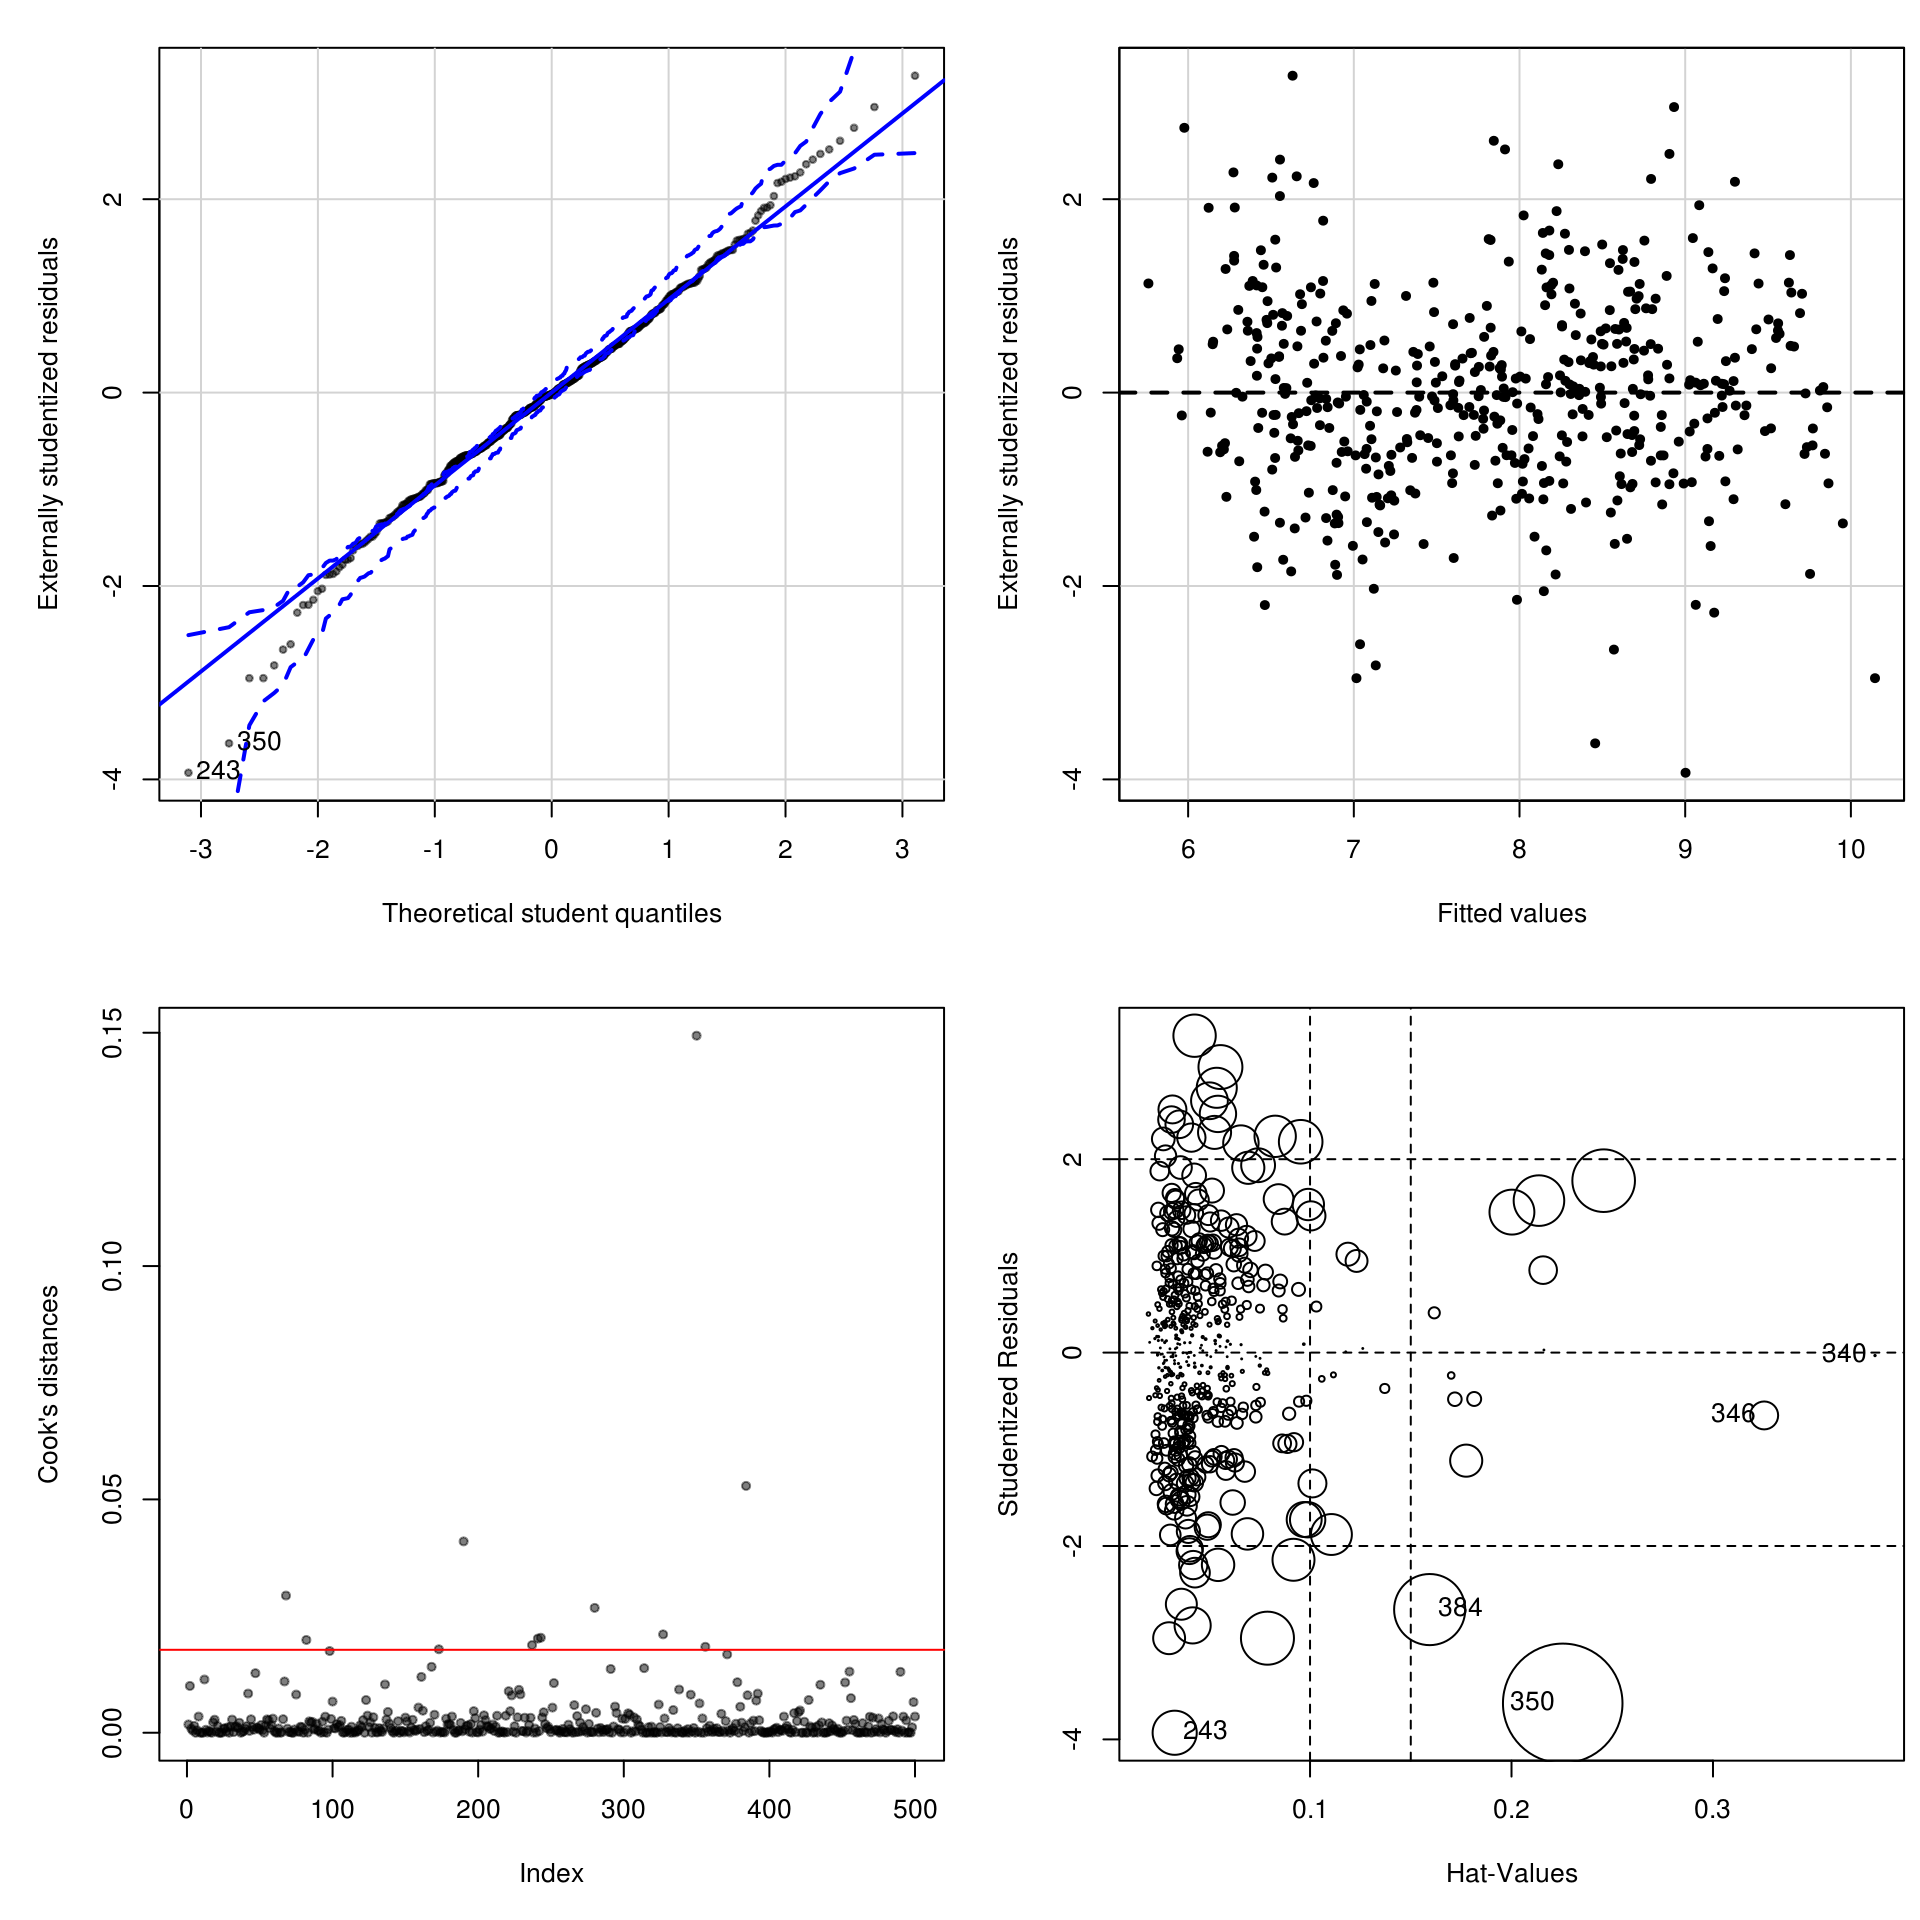
\includegraphics[width=0.7\linewidth]{LineaRModels_files/figure-latex/diagnosticsdiamonds-1} \end{center}

\begin{verbatim}
##         StudRes        Hat         CookD
## 243 -3.93155877 0.03281988 0.02036095303
## 340 -0.03069107 0.38041277 0.00002318201
## 346 -0.64996148 0.32541064 0.00816123471
## 350 -3.62756784 0.22541782 0.14936005917
## 384 -2.65776683 0.15938312 0.05289674514
\end{verbatim}

Many points have high leverage and large Cook's values. This means the slope could in principle largely be driven by those points
We get a very large residual (observation \texttt{350}, which is a very small diamond of high quality sold for almost double the value of a comparable one). A more careful analysis would be necessary to see the impact of these points on the coefficients and whether they matter (or not). For example, we could refit the model using the command \texttt{lm(final\_mod,\ subset\ =\ -350)}.

Diagnostics of heteroscedasticity are mostly useful when you have suspicions that different subgroups could have different variances (if you include factor variables) or if the data are time series, in which case you may wish to look at plots of the correlogram (\texttt{acf(resid(final\_mod))} and partial correlogram \texttt{pacf(resid(final\_mod))}). These are only useful for time ordered observations, i.e.~when the errors at time \(t\) depend on previous time periods \(\{t-1, \ldots\}\). The impact of serial dependence of the residuals is that the standard errors from OLS are too small and need to be inflated.

\hypertarget{model-selection-invalidates-p-values}{%
\section{Model selection invalidates P-values}\label{model-selection-invalidates-p-values}}

Variable selection invalidates the usual Student and Fisher tests. To see this,
we can generate a dataset \(\boldsymbol{y} = \boldsymbol{\varepsilon}\) and create an \(n \times p\) design matrix \(\mathbf{X}\) with random uncorrelated elements. We can assess
by means of simulation the size distortion (the difference between the nominal level and the type I error) of a \(t\) test for the hypothesis \(\beta_j=0\) after performing forward selection.

We illustrate the computations using two models: one in which the variables in the design matrix, \(\mathbf{X}\), are strongly correlated and another with independent input using BIC and Mallow's \(C_p\) as selection criterion. The size distortion is comparable.

\begin{verbatim}
## Uncorrelated variables, model selection using BIC
\end{verbatim}

\begin{verbatim}
##                   size
## model                 0.1   0.05   0.01
##   Lowest BIC model 0.1738 0.1076 0.0324
##   Correct model    0.1104 0.0562 0.0106
\end{verbatim}

\begin{center}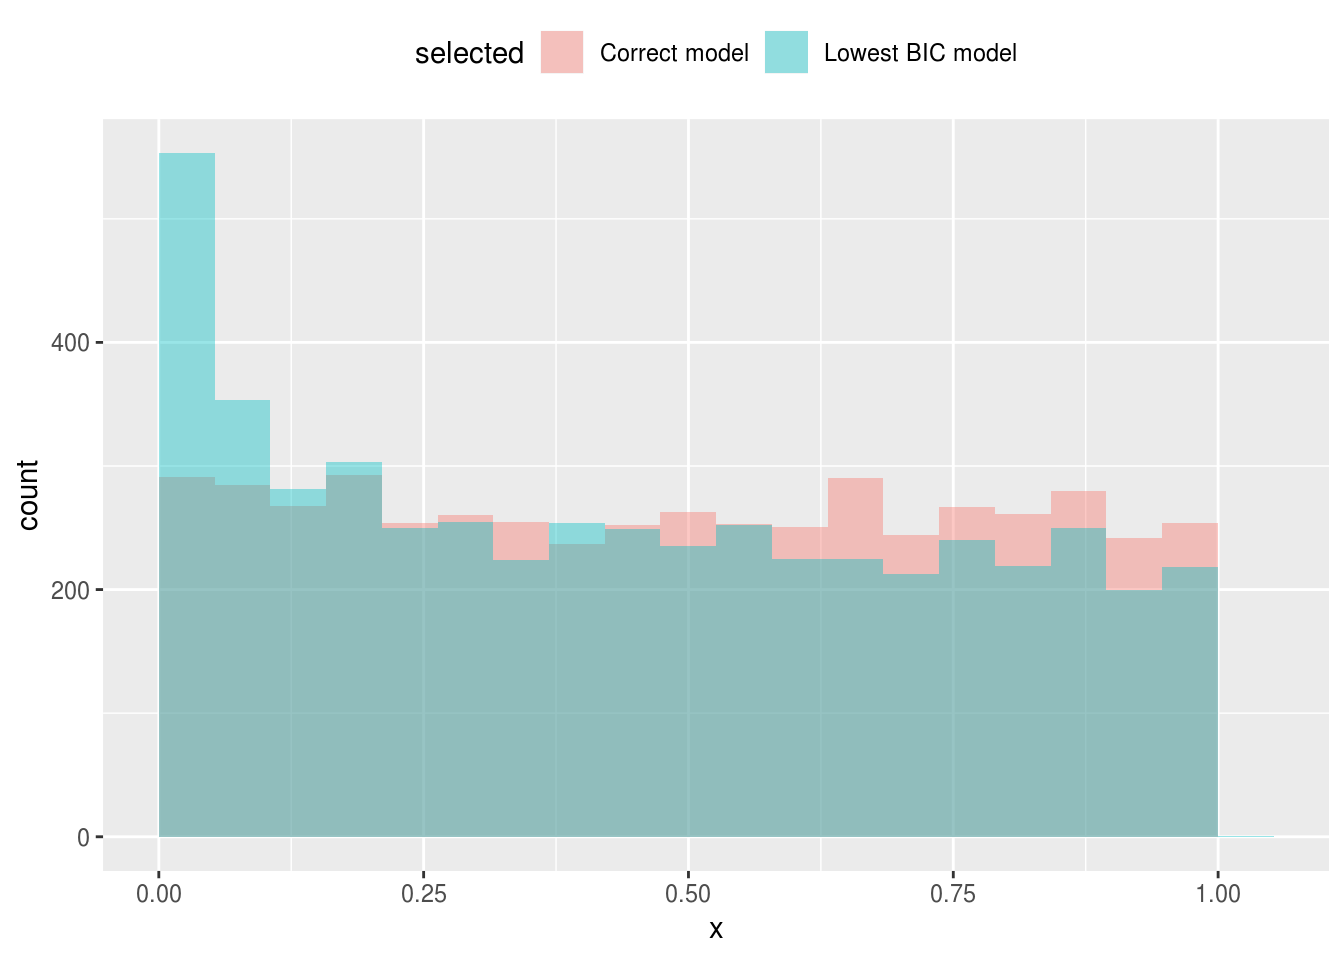
\includegraphics[width=0.7\linewidth]{LineaRModels_files/figure-latex/modelselectinvalid-1} \end{center}

\begin{verbatim}
## Correlated variables, model selection using BIC
\end{verbatim}

\begin{verbatim}
##                   size
## model                 0.1   0.05   0.01
##   Lowest BIC model 0.1846 0.1150 0.0344
##   Correct model    0.1018 0.0504 0.0110
\end{verbatim}

\begin{verbatim}
## Uncorrelated variables, model selection using Mallow's Cp
\end{verbatim}

\begin{verbatim}
##                  size
## model                0.1   0.05   0.01
##   Lowest Cp model 0.1844 0.1096 0.0318
##   Correct model   0.0978 0.0472 0.0088
\end{verbatim}

\begin{verbatim}
## Correlated variables, model selection using Mallow's Cp
\end{verbatim}

\begin{verbatim}
##                  size
## model                0.1   0.05   0.01
##   Lowest Cp model 0.1864 0.1114 0.0352
##   Correct model   0.1014 0.0514 0.0084
\end{verbatim}

\begin{center}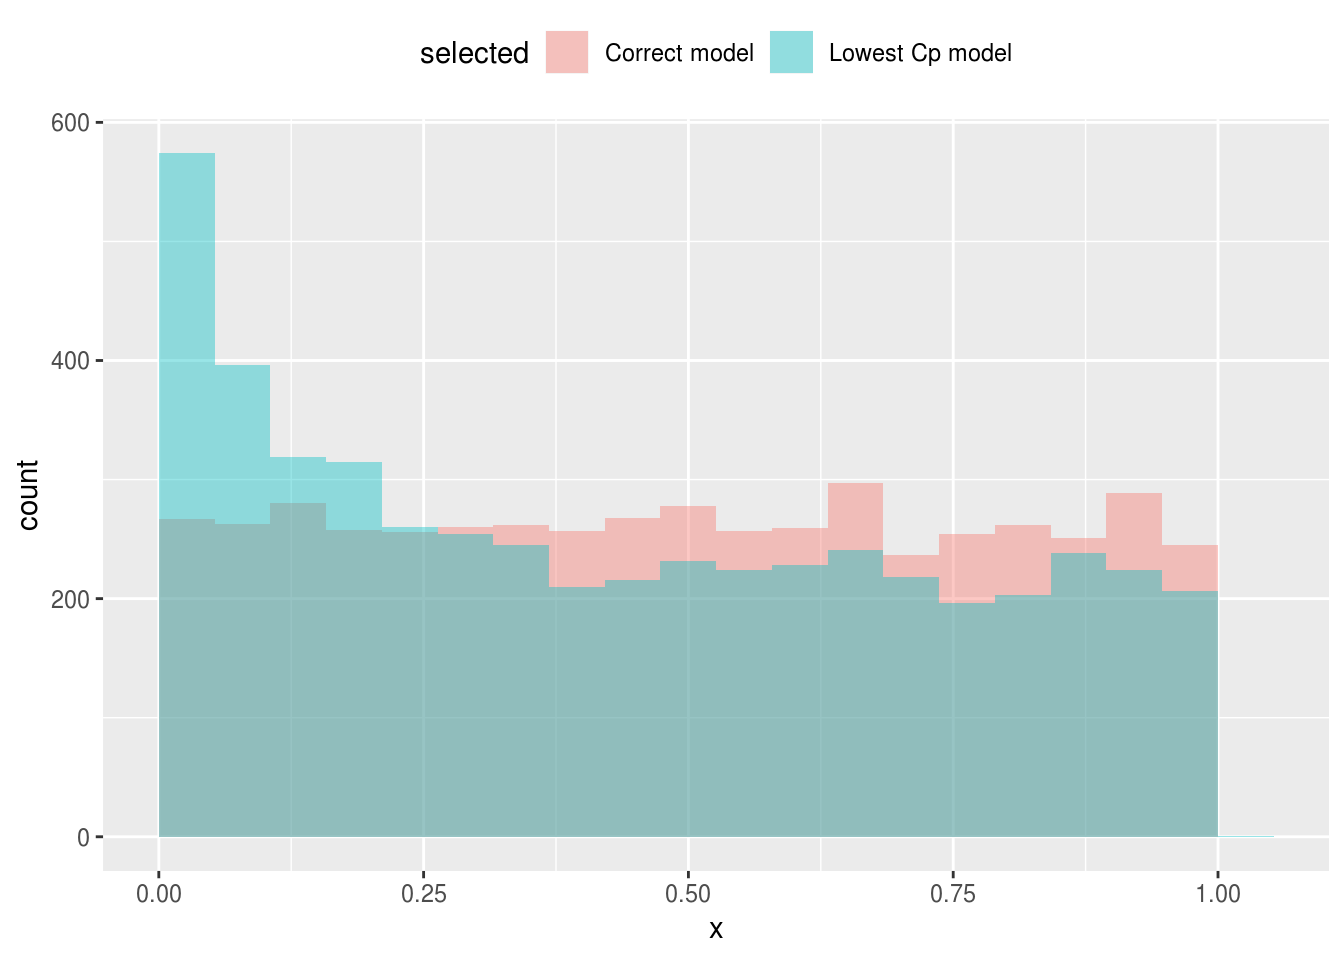
\includegraphics[width=0.7\linewidth]{LineaRModels_files/figure-latex/modelselectinvalid-2} \end{center}

Adding superfluous variables does not induce bias, but inflates the standard errors (leading to larger \(P\)-values). We observe on the contrary here smaller \(P\)-values. Recall that the \(P\)-values should be uniformly distributed under the null hypothesis (and they seemingly are when the true null model is fitted).

\hypertarget{penalized-regression-methods}{%
\chapter{Penalized regression methods}\label{penalized-regression-methods}}

There are two reasons one may go down the route of penalized regression models: one is to trade-off bias for reduced variance in the hope that doing so will improve the predictive accuracy of the model. The other is in cases where the number of covariates \(p\) is large and the matrix \(\mathbf{X}\) is close to being non-invertible.

Throughout, we will work with centered and standardized inputs. One reason for doing so is to make our inference invariant to affine transformations, much like for \(R^2_c\). We can consider a design matrix \([ \mathbf{1}_n \; \mathbf{X}]\) with rescaled columns so that \(\mathrm{Var}(\mathbf{X}_j)=1\) for \(j=1, \ldots, p\) and take \(\mathbf{Z} \equiv \mathbf{X} - \mathbf{1}_n \bar{\mathbf{X}}\), where \(\bar{\mathbf{X}}\) is the row vector of column means of \(\mathbf{X}\). This is the orthogonal decomposition \(\mathbf{H}_{\mathbf{1}_n} + \mathbf{H}_{\mathbf{M}_{\mathbf{1}_n}\mathbf{X}}\) and since the variables are orthogonal, the coefficient \(\beta_0\) corresponding to the intercept is \(\bar{\boldsymbol{y}}\).
Having scaled inputs \(\mathbf{Z}\) ensures that we penalize equally every covariate and that the model is invariant to change of units for the regressors.

The two methods briefly covered in the course are ridge regression and LASSO. The first one consists of imposing a \(l_2\) penalty on the coefficients, the second a \(l_1\) penalty. The advantage of the former is that the optimization problem is convex and differentiable and the solution can be found using an augmented linear regression. We will solely focus on ridge regression in the sequel.

Our objective function for ridge regression takes the form
\[Q(\beta_0, \boldsymbol{\gamma}) = (\boldsymbol{y} - \beta_0 \mathbf{1}_n -\mathbf{Z}\boldsymbol{\gamma})^\top(\boldsymbol{y} - \beta_0 \mathbf{1}_n -\mathbf{Z}\boldsymbol{\gamma}) + \lambda \|\boldsymbol{\gamma}\|^2_2. \]

\hypertarget{bias-and-variance-tradeoff}{%
\section{Bias and variance tradeoff}\label{bias-and-variance-tradeoff}}

As we increase the penalty \(\lambda\), the values of the ridge coefficients are shrunk towards zero. The case \(\lambda \to \infty\) gives \(\hat{\boldsymbol{\beta}}_{\mathrm{ridge}}=\boldsymbol{0}_p\), whereas we retrieve the OLS estimator \(\hat{\boldsymbol{\beta}}\) when \(\lambda=0\).

The mean squared error of the ridge estimator is
\begin{align*}
\mathrm{MSE}(\hat{\boldsymbol{\beta}}_{\mathrm{ridge}}^{\lambda}) &= \sigma^2 \mathrm{tr}\left\{(\mathbf{Z}^\top\mathbf{Z} + \lambda \mathbf{I}_p)^{-1}\mathbf{Z}^\top\mathbf{Z}(\mathbf{Z}^\top\mathbf{Z} + \lambda \mathbf{I}_p)^{-1}\right\} \\&\quad + \boldsymbol{\gamma}^\top \left\{ \mathbf{Z}^\top\mathbf{Z}(\mathbf{Z}^\top\mathbf{Z} + \lambda \mathbf{I}_p)^{-1} + \mathbf{I}_p \right\} \left\{ (\mathbf{Z}^\top\mathbf{Z} + \lambda \mathbf{I}_p)^{-1}\mathbf{Z}^\top\mathbf{Z} + \mathbf{I}_p \right\}\boldsymbol{\gamma}
\end{align*}

If we knew the true data generating mechanism (i.e.~the \(\boldsymbol{\gamma}\) vector and \(\sigma^2\)), we could compute exactly the mean squared error (MSE) of the model and find the optimal bias-variance tradeoff that minimizes MSE. This is illustrated below in an artificial example. As \(\lambda \to \infty\), the bias grows and dominates MSE.

\begin{Shaded}
\begin{Highlighting}[]
\CommentTok{# Function to compute MSE of ridge estimator}
\NormalTok{mse_ridge <-}\StringTok{ }\ControlFlowTok{function}\NormalTok{(gamma, lambda, Z, }\DataTypeTok{sigmasq =} \DecValTok{1}\NormalTok{)\{}
\NormalTok{  ZtZ <-}\StringTok{ }\KeywordTok{crossprod}\NormalTok{(Z)}
\NormalTok{  p <-}\StringTok{ }\KeywordTok{ncol}\NormalTok{(Z)}
\NormalTok{  W <-}\StringTok{ }\KeywordTok{solve}\NormalTok{(ZtZ }\OperatorTok{+}\StringTok{ }\NormalTok{lambda}\OperatorTok{*}\KeywordTok{diag}\NormalTok{(p))}
\NormalTok{  bias <-}\StringTok{ }\KeywordTok{c}\NormalTok{((W }\OperatorTok\StringTok{ }\NormalTok{ZtZ }\OperatorTok{-}\StringTok{ }\KeywordTok{diag}\NormalTok{(p)) }\OperatorTok\StringTok{ }\NormalTok{gamma)}
\NormalTok{  varia <-}\StringTok{ }\NormalTok{sigmasq }\OperatorTok{*}\StringTok{ }\KeywordTok{diag}\NormalTok{( }\KeywordTok{crossprod}\NormalTok{(Z }\OperatorTok\StringTok{ }\NormalTok{W))}
  \KeywordTok{list}\NormalTok{(}\DataTypeTok{bias =}\NormalTok{ bias, }\DataTypeTok{variance =}\NormalTok{ varia, }\DataTypeTok{mse =} \KeywordTok{sum}\NormalTok{(bias}\OperatorTok{^}\DecValTok{2} \OperatorTok{+}\StringTok{ }\NormalTok{varia))}
\NormalTok{\}}
\KeywordTok{set.seed}\NormalTok{(}\DecValTok{9876}\NormalTok{)}
\CommentTok{# Create fake data}
\NormalTok{Z <-}\StringTok{ }\KeywordTok{matrix}\NormalTok{(}\KeywordTok{rnorm}\NormalTok{(}\DataTypeTok{n =}\NormalTok{ 20L}\OperatorTok{*}\NormalTok{50L, }\DataTypeTok{mean =} \DecValTok{0}\NormalTok{, }\DataTypeTok{sd =} \DecValTok{1}\NormalTok{), }\DataTypeTok{ncol =}\NormalTok{ 20L)}
\CommentTok{# Center and renormalize Z}
\NormalTok{Z <-}\StringTok{ }\KeywordTok{apply}\NormalTok{(Z, }\DecValTok{2}\NormalTok{, scale)}
\CommentTok{# Create coefficient vector}
\NormalTok{gamma <-}\StringTok{ }\KeywordTok{c}\NormalTok{(}\KeywordTok{rep}\NormalTok{(}\DecValTok{0}\NormalTok{, 10L), }\KeywordTok{runif}\NormalTok{(10L))}

\CommentTok{# Create sequence of lambda and matrix to store results}
\NormalTok{nlam <-}\StringTok{ }\NormalTok{401L}
\NormalTok{lambda_seq <-}\StringTok{ }\KeywordTok{seq}\NormalTok{(}\DecValTok{0}\NormalTok{, }\DecValTok{100}\NormalTok{, }\DataTypeTok{length =}\NormalTok{ nlam)}
\NormalTok{mse <-}\StringTok{ }\KeywordTok{matrix}\NormalTok{(}\DecValTok{0}\NormalTok{, }\DataTypeTok{nrow =}\NormalTok{ nlam, }\DataTypeTok{ncol =} \DecValTok{3}\NormalTok{)}
\NormalTok{gammahat <-}\StringTok{ }\KeywordTok{matrix}\NormalTok{(}\DecValTok{0}\NormalTok{, }\DataTypeTok{nrow =}\NormalTok{ nlam, }\DataTypeTok{ncol =} \KeywordTok{ncol}\NormalTok{(Z))}
\ControlFlowTok{for}\NormalTok{(i }\ControlFlowTok{in} \DecValTok{1}\OperatorTok{:}\NormalTok{nlam)\{}
  \CommentTok{# evaluate bias + variance for each lambda}
\NormalTok{  mse_i <-}\StringTok{ }\KeywordTok{mse_ridge}\NormalTok{(}\DataTypeTok{gamma =}\NormalTok{ gamma, }\DataTypeTok{lambda =}\NormalTok{ lambda_seq[i], }\DataTypeTok{Z =}\NormalTok{ Z)}
\NormalTok{  gammahat[i,] <-}\StringTok{ }\NormalTok{gamma }\OperatorTok{+}\StringTok{ }\NormalTok{mse_i}\OperatorTok{$}\NormalTok{bias}
\NormalTok{  mse[i,}\DecValTok{1}\NormalTok{] <-}\StringTok{  }\KeywordTok{sum}\NormalTok{(mse_i}\OperatorTok{$}\NormalTok{bias}\OperatorTok{^}\DecValTok{2}\NormalTok{)}
\NormalTok{  mse[i,}\DecValTok{2}\NormalTok{] <-}\StringTok{  }\KeywordTok{sum}\NormalTok{(mse_i}\OperatorTok{$}\NormalTok{variance)}
\NormalTok{  mse[i,}\DecValTok{3}\NormalTok{] <-}\StringTok{ }\NormalTok{mse_i}\OperatorTok{$}\NormalTok{mse}
\NormalTok{\}}
\CommentTok{# Plot the results as a function of lambda}
\KeywordTok{matplot}\NormalTok{(lambda_seq, mse, }\DataTypeTok{type =} \StringTok{"l"}\NormalTok{, }\DataTypeTok{lty =} \DecValTok{1}\NormalTok{, }
        \DataTypeTok{bty =} \StringTok{"l"}\NormalTok{, }\DataTypeTok{xlab =} \KeywordTok{expression}\NormalTok{(lambda), }\DataTypeTok{col =} \DecValTok{3}\OperatorTok{:}\DecValTok{1}\NormalTok{, }
        \DataTypeTok{ylab =} \StringTok{"Mean squared error decomposition"}\NormalTok{)}
\KeywordTok{abline}\NormalTok{(}\DataTypeTok{h =}\NormalTok{ mse[}\DecValTok{1}\NormalTok{,}\DecValTok{3}\NormalTok{], }\DataTypeTok{lty =} \DecValTok{2}\NormalTok{)}
\KeywordTok{legend}\NormalTok{(}\DataTypeTok{x =} \StringTok{"topleft"}\NormalTok{, }\DataTypeTok{legend =} \KeywordTok{c}\NormalTok{(}\StringTok{"sq. bias"}\NormalTok{, }\StringTok{"variance"}\NormalTok{, }\StringTok{"mse"}\NormalTok{), }
       \DataTypeTok{col =} \DecValTok{3}\OperatorTok{:}\DecValTok{1}\NormalTok{, }\DataTypeTok{lty =} \DecValTok{1}\NormalTok{, }\DataTypeTok{bty =} \StringTok{"n"}\NormalTok{)}
\end{Highlighting}
\end{Shaded}

\begin{center}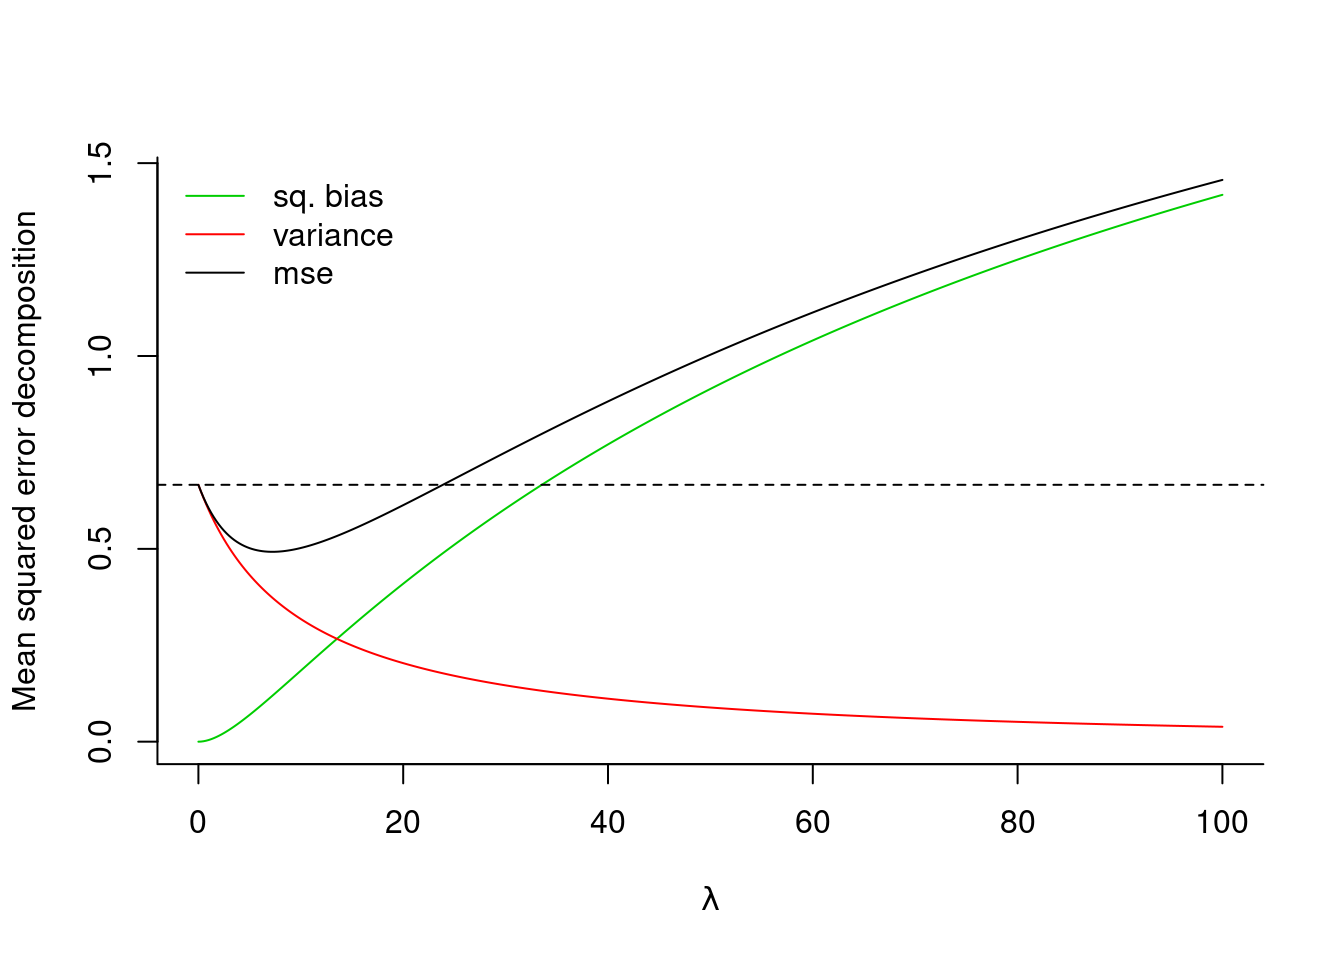
\includegraphics[width=0.7\linewidth]{LineaRModels_files/figure-latex/biasridge-1} \end{center}

\begin{Shaded}
\begin{Highlighting}[]
\CommentTok{# Compute the value of lambda that minimizes MSE}
\NormalTok{lambdaopt <-}\StringTok{ }\KeywordTok{optimize}\NormalTok{(}\DataTypeTok{f =} \ControlFlowTok{function}\NormalTok{(x)\{}
  \KeywordTok{mse_ridge}\NormalTok{(}\DataTypeTok{gamma =}\NormalTok{ gamma, }\DataTypeTok{lambda =}\NormalTok{ x, }\DataTypeTok{Z =}\NormalTok{ Z)}\OperatorTok{$}\NormalTok{mse}
\NormalTok{  \}, }\DataTypeTok{interval =} \KeywordTok{c}\NormalTok{(}\DecValTok{0}\NormalTok{, }\DecValTok{30}\NormalTok{))}\OperatorTok{$}\NormalTok{minimum}
\NormalTok{lambdaopt}
\end{Highlighting}
\end{Shaded}

\begin{verbatim}
## [1] 7.227898
\end{verbatim}

We can also look at the path of coefficient values \(\hat{\boldsymbol{\gamma}}_{\mathrm{ridge}}^{\lambda}\) as a function of \(\lambda\):

\begin{center}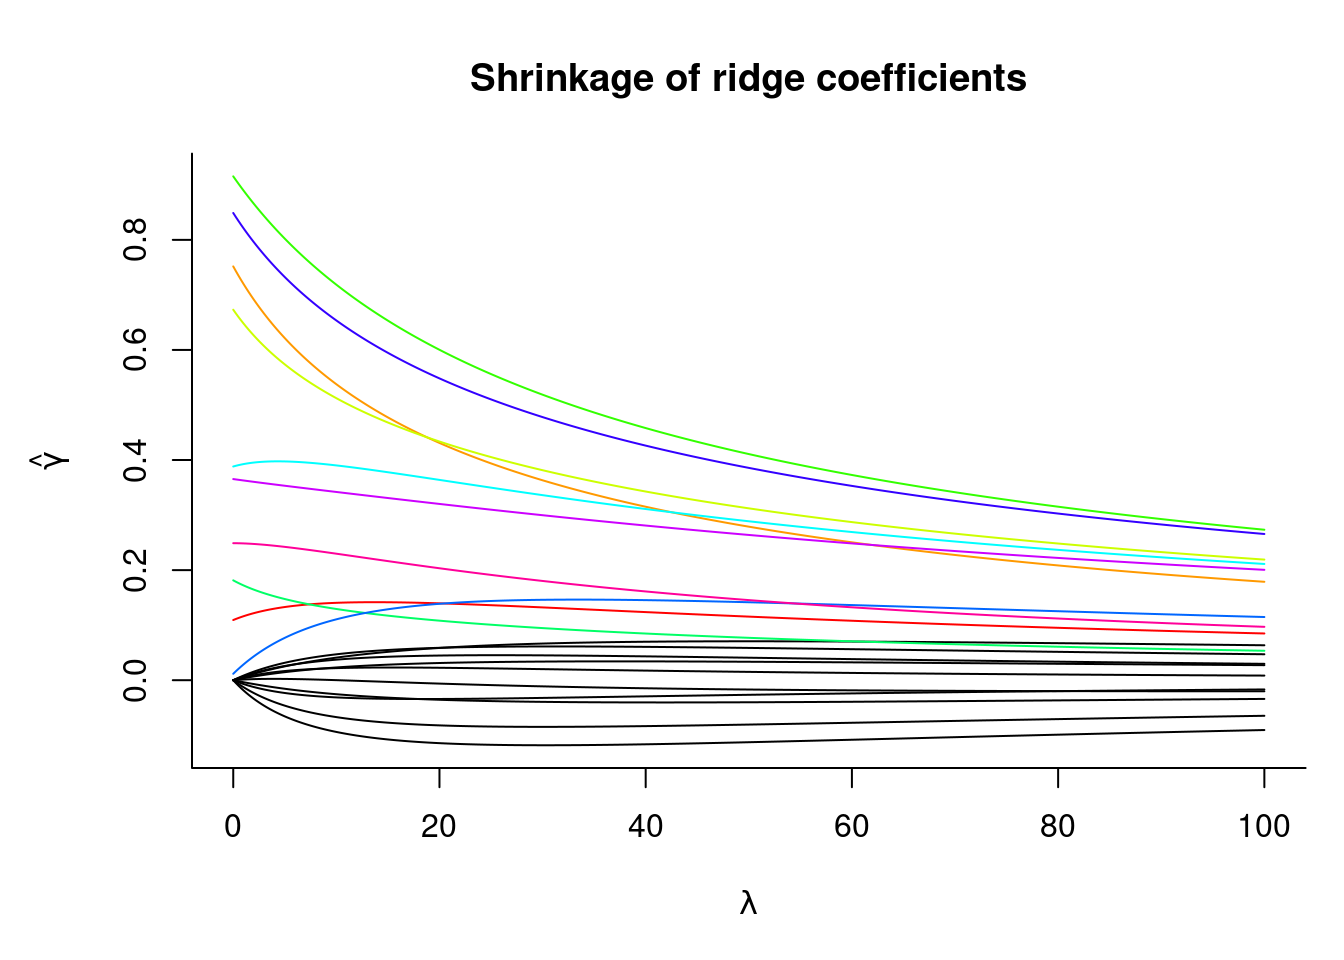
\includegraphics[width=0.7\linewidth]{LineaRModels_files/figure-latex/plotgammaridge-1} \end{center}

While the overall vector of coefficients are shrunk towards zero, the set of 10 first coefficients \(\boldsymbol{\gamma}\), which are exactly zero, stabilize around another value. Note that if we increase the penalty, from \(\lambda_1\) to \(\lambda_2\) with \(\lambda_1 < \lambda_2\), this \textbf{does not} necessarily imply that individual coefficient estimates decrease, i.e.~\(|\hat{\beta}_j (\lambda_1)| \nleq |\hat{\beta}_j(\lambda_2)|\) even if \(\lambda_1 < \lambda_2\).

The coefficients \(\hat{\boldsymbol{\gamma}}^\lambda\) can be computed using an augmented linear regression, with response \((\boldsymbol{y}, \mathbf{0}_p)\) and regressor \([\mathbf{Z}^\top,\; \lambda^{1/2} \mathbf{I}_p]\). Alternatively,
\[\hat{\boldsymbol{\gamma}}^\lambda = (\mathbf{Z}^\top\mathbf{Z} + \lambda \mathbf{I}_p)^{-1}\mathbf{Z}^\top\boldsymbol{y}.\]

We can also use the singular value decomposition of \(\mathbf{Z} = \mathbf{UDV}^\top\) to compute the coefficients\[\hat{\boldsymbol{\gamma}} = \sum_{j=1}^p \frac{d_j}{d_j^2+\lambda} \mathbf{u}_j^\top\boldsymbol{y} \mathbf{v}_j,\]
where \(\mathbf{u}_j\) and \(\mathbf{v}_j\) are the \(j\)th column of \(\mathbf{U}\) and \(\mathbf{V}\), respectively. This is most useful for cross-validation where we want to change the value of \(\lambda\) repeatedly, as the SVD of \(\mathbf{Z}\) won't change.

\begin{Shaded}
\begin{Highlighting}[]
\CommentTok{# Create response vector from model}
\NormalTok{y <-}\StringTok{ }\NormalTok{Z }\OperatorTok\StringTok{ }\NormalTok{gamma }\OperatorTok{+}\StringTok{ }\KeywordTok{rnorm}\NormalTok{(}\KeywordTok{nrow}\NormalTok{(Z))}
\CommentTok{# Compute ridge coefficients}
\NormalTok{ridge_lm_coef <-}\StringTok{ }\ControlFlowTok{function}\NormalTok{(y, Z, lambda)\{}
\NormalTok{ Z <-}\StringTok{ }\KeywordTok{scale}\NormalTok{(Z) }
 \KeywordTok{c}\NormalTok{(}\KeywordTok{solve}\NormalTok{(}\KeywordTok{crossprod}\NormalTok{(Z) }\OperatorTok{+}\StringTok{ }\NormalTok{lambda}\OperatorTok{*}\KeywordTok{diag}\NormalTok{(}\KeywordTok{ncol}\NormalTok{(Z))) }\OperatorTok\StringTok{ }\KeywordTok{crossprod}\NormalTok{(Z, y }\OperatorTok{-}\StringTok{ }\KeywordTok{mean}\NormalTok{(y)))}
\NormalTok{\}}
\NormalTok{lambda0 <-}\StringTok{ }\DecValTok{2}
\CommentTok{#Compare coefficients obtained from fitting using augmented regression}
\NormalTok{augmy <-}\StringTok{ }\KeywordTok{c}\NormalTok{(y }\OperatorTok{-}\StringTok{ }\KeywordTok{mean}\NormalTok{(y), }\KeywordTok{rep}\NormalTok{(}\DecValTok{0}\NormalTok{, }\KeywordTok{ncol}\NormalTok{(Z)))}
\NormalTok{augmZ <-}\StringTok{ }\KeywordTok{rbind}\NormalTok{(Z, }\KeywordTok{sqrt}\NormalTok{(lambda0)}\OperatorTok{*}\KeywordTok{diag}\NormalTok{(}\KeywordTok{ncol}\NormalTok{(Z)))}
\NormalTok{augmlm <-}\StringTok{ }\KeywordTok{lm}\NormalTok{(augmy }\OperatorTok{~}\StringTok{ }\DecValTok{-1} \OperatorTok{+}\StringTok{ }\NormalTok{augmZ)}
\KeywordTok{isTRUE}\NormalTok{(}\KeywordTok{all.equal}\NormalTok{(}\KeywordTok{as.vector}\NormalTok{(augmlm}\OperatorTok{$}\NormalTok{coef),}
      \KeywordTok{ridge_lm_coef}\NormalTok{(}\DataTypeTok{y =}\NormalTok{ y, }\DataTypeTok{Z =}\NormalTok{ Z, }\DataTypeTok{lambda =}\NormalTok{ lambda0)))}
\end{Highlighting}
\end{Shaded}

\begin{verbatim}
## [1] TRUE
\end{verbatim}

\hypertarget{cross-validation-1}{%
\section{Cross-validation}\label{cross-validation-1}}

Denote the ridge estimator \(\hat{\boldsymbol{\beta}}^\lambda\) for a given penalty parameter \(\lambda\).
The smoothing matrix, as given in the course notes, is \[\mathbf{S}_{\lambda} = \mathbf{Z}(\mathbf{Z}^\top\mathbf{Z} + \lambda \mathbf{I}_p)^{-1}\mathbf{Z}^\top;\] its trace is \(\mathrm{tr}({\mathbf{S}_{\lambda}}) = \sum_{j=1}^p d_j^2/(d_j^2+\lambda)\), where \(d_{j}\) is the \(j\)th singular value of \(\mathbf{Z}\). The smoothing matrix \(\mathbf{S}_{\lambda}\) is not a projection matrix; its eigenvalues lie in \((0,1)\).

Similar calculations than those used to derive the leave-one-out cross validation residual errors of the PRESS statistic lead to the formula
\[\mathrm{CV}_\lambda = \sum_{i=1}^n e_{-i}^2(\lambda) =  \sum_{i=1}^n (y_i - \bar{y}- \mathbf{z}_i \hat{\boldsymbol{\gamma}}_{-i}^{\lambda})^2 = \sum_{i=1}^n \frac{(y_i - \bar{y} -\mathbf{z}_i\hat{\boldsymbol{\gamma}}^\lambda)^2}{1-{\mathbf{S}_{\lambda}}_{ii}},\]
where \(\mathbf{z}_i\) is the \(i\)th row of \(\mathbf{Z}\).
Rather than compute \(\mathbf{S}_{\lambda}\) and its diagonal elements, one can resort to the convenient generalized cross-validation approximation
\[\mathrm{GCV}_\lambda = \sum_{i=1}^n \frac{(y_i - \bar{y} -\mathbf{z}_i\hat{\boldsymbol{\gamma}}^\lambda)^2}{1-\mathrm{tr}(\mathbf{S}_{\lambda})/n}\]
and the latter is readily computed.

\begin{Shaded}
\begin{Highlighting}[]
\NormalTok{nlam <-}\StringTok{ }\NormalTok{201L}
\NormalTok{lambda_seq <-}\StringTok{ }\KeywordTok{seq}\NormalTok{(}\DecValTok{0}\NormalTok{, }\DecValTok{20}\NormalTok{, }\DataTypeTok{length =}\NormalTok{ nlam)}
\NormalTok{svdZ <-}\StringTok{ }\KeywordTok{svd}\NormalTok{(Z)}
\NormalTok{n <-}\StringTok{ }\KeywordTok{nrow}\NormalTok{(Z); p <-}\StringTok{ }\KeywordTok{ncol}\NormalTok{(Z)}
\CommentTok{#Each column is u_j^Tyv_j}
\NormalTok{uyv <-}\StringTok{ }\KeywordTok{sapply}\NormalTok{(}\DecValTok{1}\OperatorTok{:}\NormalTok{p, }\ControlFlowTok{function}\NormalTok{(j)\{}\KeywordTok{t}\NormalTok{(svdZ}\OperatorTok{$}\NormalTok{u[,j]) }\OperatorTok\StringTok{ }\NormalTok{y }\OperatorTok\StringTok{ }\NormalTok{svdZ}\OperatorTok{$}\NormalTok{v[,j]\})}
\NormalTok{gcv <-}\StringTok{ }\KeywordTok{rep}\NormalTok{(}\DecValTok{0}\NormalTok{, nlam)}
\NormalTok{yc <-}\StringTok{ }\NormalTok{y }\OperatorTok{-}\StringTok{ }\KeywordTok{mean}\NormalTok{(y)}
\ControlFlowTok{for}\NormalTok{(i }\ControlFlowTok{in} \DecValTok{1}\OperatorTok{:}\NormalTok{nlam)\{}
  \CommentTok{# Compute GCV - trace of smoother + RSS}
\NormalTok{  traceS <-}\StringTok{ }\KeywordTok{sum}\NormalTok{(svdZ}\OperatorTok{$}\NormalTok{d}\OperatorTok{^}\DecValTok{2}\OperatorTok{/}\NormalTok{(svdZ}\OperatorTok{$}\NormalTok{d}\OperatorTok{^}\DecValTok{2}\OperatorTok{+}\NormalTok{lambda_seq[i]))}
\NormalTok{  gcv[i] <-}\StringTok{ }\KeywordTok{sum}\NormalTok{((yc }\OperatorTok{-}\StringTok{ }\NormalTok{Z }\OperatorTok\StringTok{ }\KeywordTok{colSums}\NormalTok{(}\KeywordTok{c}\NormalTok{(svdZ}\OperatorTok{$}\NormalTok{d}\OperatorTok{/}\NormalTok{(svdZ}\OperatorTok{$}\NormalTok{d}\OperatorTok{^}\DecValTok{2} \OperatorTok{+}\StringTok{ }\NormalTok{lambda_seq[i]))  }\OperatorTok{*}
\StringTok{                                      }\KeywordTok{t}\NormalTok{(uyv)))}\OperatorTok{^}\DecValTok{2}\NormalTok{)}\OperatorTok{/}\NormalTok{(}\DecValTok{1}\OperatorTok{-}\NormalTok{traceS}\OperatorTok{/}\NormalTok{n)}\OperatorTok{^}\DecValTok{2}
\NormalTok{\}}
\CommentTok{# Plot GCV curve against lambda}
\KeywordTok{plot}\NormalTok{(lambda_seq, gcv, }\DataTypeTok{type =} \StringTok{"l"}\NormalTok{, }\DataTypeTok{bty =} \StringTok{"l"}\NormalTok{,}
     \DataTypeTok{main =} \StringTok{"Generalized leave-one-out}\CharTok{\textbackslash{}n}\StringTok{cross validation for ridge regression"}\NormalTok{,}
     \DataTypeTok{ylab =} \KeywordTok{expression}\NormalTok{(GCV[lambda]), }\DataTypeTok{xlab =} \KeywordTok{expression}\NormalTok{(lambda))}
\KeywordTok{abline}\NormalTok{(}\DataTypeTok{v =}\NormalTok{ lambda_seq[}\KeywordTok{which.min}\NormalTok{(gcv)], }\DataTypeTok{col =} \DecValTok{2}\NormalTok{)}
\NormalTok{lambda_seq[}\KeywordTok{which.min}\NormalTok{(gcv)]}
\end{Highlighting}
\end{Shaded}

\begin{verbatim}
## [1] 13.5
\end{verbatim}

\begin{Shaded}
\begin{Highlighting}[]
\CommentTok{# Compare results with MASS}
\KeywordTok{library}\NormalTok{(MASS)}
\NormalTok{fit_ridge <-}\StringTok{ }\KeywordTok{lm.ridge}\NormalTok{(y }\OperatorTok{~}\StringTok{ }\NormalTok{Z, }\DataTypeTok{lambda =}\NormalTok{ lambda_seq)}
\CommentTok{# GCV returned by lm.ridge is divided by n^2}
\KeywordTok{lines}\NormalTok{(lambda_seq, fit_ridge}\OperatorTok{$}\NormalTok{GCV}\OperatorTok{*}\NormalTok{n}\OperatorTok{^}\DecValTok{2}\NormalTok{, }\DataTypeTok{lty =} \DecValTok{2}\NormalTok{, }\DataTypeTok{col =} \StringTok{"blue"}\NormalTok{)}
\end{Highlighting}
\end{Shaded}

\begin{center}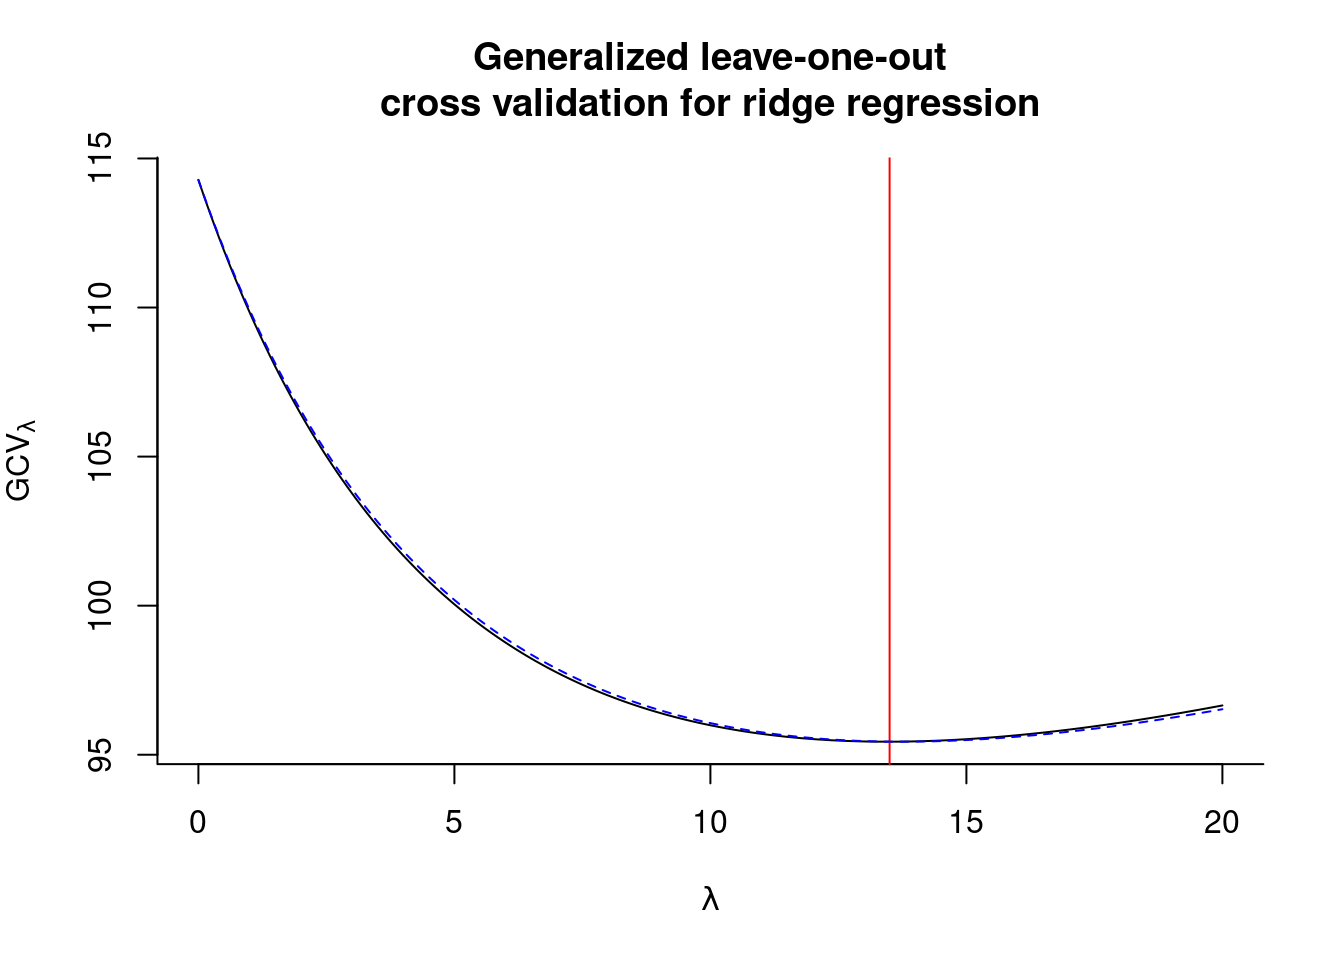
\includegraphics[width=0.7\linewidth]{LineaRModels_files/figure-latex/gcv_ridge-1} \end{center}

\begin{Shaded}
\begin{Highlighting}[]
\KeywordTok{select}\NormalTok{(fit_ridge)}
\end{Highlighting}
\end{Shaded}

\begin{verbatim}
## modified HKB estimator is 8.577316 
## modified L-W estimator is 7.881568 
## smallest value of GCV  at 13.7
\end{verbatim}

Note that in this case, the optimal value of \(\lambda\) found is higher than the theoretical optimum. In practice, we may prefer \(K\)-fold cross-validation to leave-one-out cross validation.

\hypertarget{splines}{%
\chapter{Splines}\label{splines}}

The following code provides functions to compute manually a cubic spline
and returns the penalty function. In \textbf{R}, one would rather use functions
that compute efficiently the generalized cross-validation criterion and return
the best smoothing or regression spline.

The package \texttt{splines} contains \texttt{bs} for cubic regression splines and \texttt{ns} for natural regression splines. Smoothing splines can be obtained by a call to \texttt{smooth.spline}.
The following illustrates a regression spline in which a number of knots (here roughly \(n/10\)) are chosen equispaced on the distribution scale, based on the quantiles of the covariate vector.

\begin{Shaded}
\begin{Highlighting}[]
\KeywordTok{library}\NormalTok{(splines)}
\KeywordTok{data}\NormalTok{(mcycle, }\DataTypeTok{package =} \StringTok{"MASS"}\NormalTok{)}
\CommentTok{# Center observations}
\NormalTok{x <-}\StringTok{ }\NormalTok{mcycle}\OperatorTok{$}\NormalTok{times}
\NormalTok{y <-}\StringTok{ }\NormalTok{mcycle}\OperatorTok{$}\NormalTok{accel }\OperatorTok{-}\StringTok{ }\KeywordTok{mean}\NormalTok{(mcycle}\OperatorTok{$}\NormalTok{accel)}
\NormalTok{n <-}\StringTok{ }\KeywordTok{length}\NormalTok{(x)}
\NormalTok{df <-}\StringTok{ }\KeywordTok{floor}\NormalTok{(n}\OperatorTok{/}\DecValTok{10}\NormalTok{)}
\CommentTok{# Compute number of knots}
\NormalTok{m <-}\StringTok{ }\NormalTok{df }\OperatorTok{+}\StringTok{ }\DecValTok{4}
\NormalTok{knots <-}\StringTok{  }\KeywordTok{quantile}\NormalTok{(x, }\DataTypeTok{prob =}\NormalTok{ (}\DecValTok{1}\OperatorTok{:}\NormalTok{m)}\OperatorTok{/}\NormalTok{(m}\OperatorTok{+}\DecValTok{1}\NormalTok{))}

\CommentTok{#With regression natural cubic spline, equispaced knots on quantile scale}
\KeywordTok{plot}\NormalTok{(y}\OperatorTok{~}\NormalTok{x, }\DataTypeTok{xlab =} \StringTok{"time after impact (in milliseconds)"}\NormalTok{, }\DataTypeTok{ylab =} \StringTok{"acceleration"}\NormalTok{,}
     \DataTypeTok{main =} \StringTok{"Simulated motorcycle accident"}\NormalTok{, }\DataTypeTok{bty =} \StringTok{"l"}\NormalTok{)}
\KeywordTok{lines}\NormalTok{(x, }\KeywordTok{fitted}\NormalTok{(}\KeywordTok{lm}\NormalTok{(y}\OperatorTok{~}\KeywordTok{ns}\NormalTok{(}\DataTypeTok{x =}\NormalTok{ x, }\DataTypeTok{knots =}\NormalTok{ knots))), }\DataTypeTok{col =} \StringTok{"red"}\NormalTok{)}
\CommentTok{#Smoothing spline, using GCV}
\NormalTok{spl <-}\StringTok{ }\KeywordTok{smooth.spline}\NormalTok{(}\DataTypeTok{x =}\NormalTok{ x, }\DataTypeTok{y =}\NormalTok{ y, }\DataTypeTok{cv =} \OtherTok{FALSE}\NormalTok{, }\DataTypeTok{all.knots =} \OtherTok{TRUE}\NormalTok{)}
\KeywordTok{lines}\NormalTok{(x, }\KeywordTok{fitted}\NormalTok{(spl), }\DataTypeTok{col =} \StringTok{"green"}\NormalTok{)}
\end{Highlighting}
\end{Shaded}

\begin{center}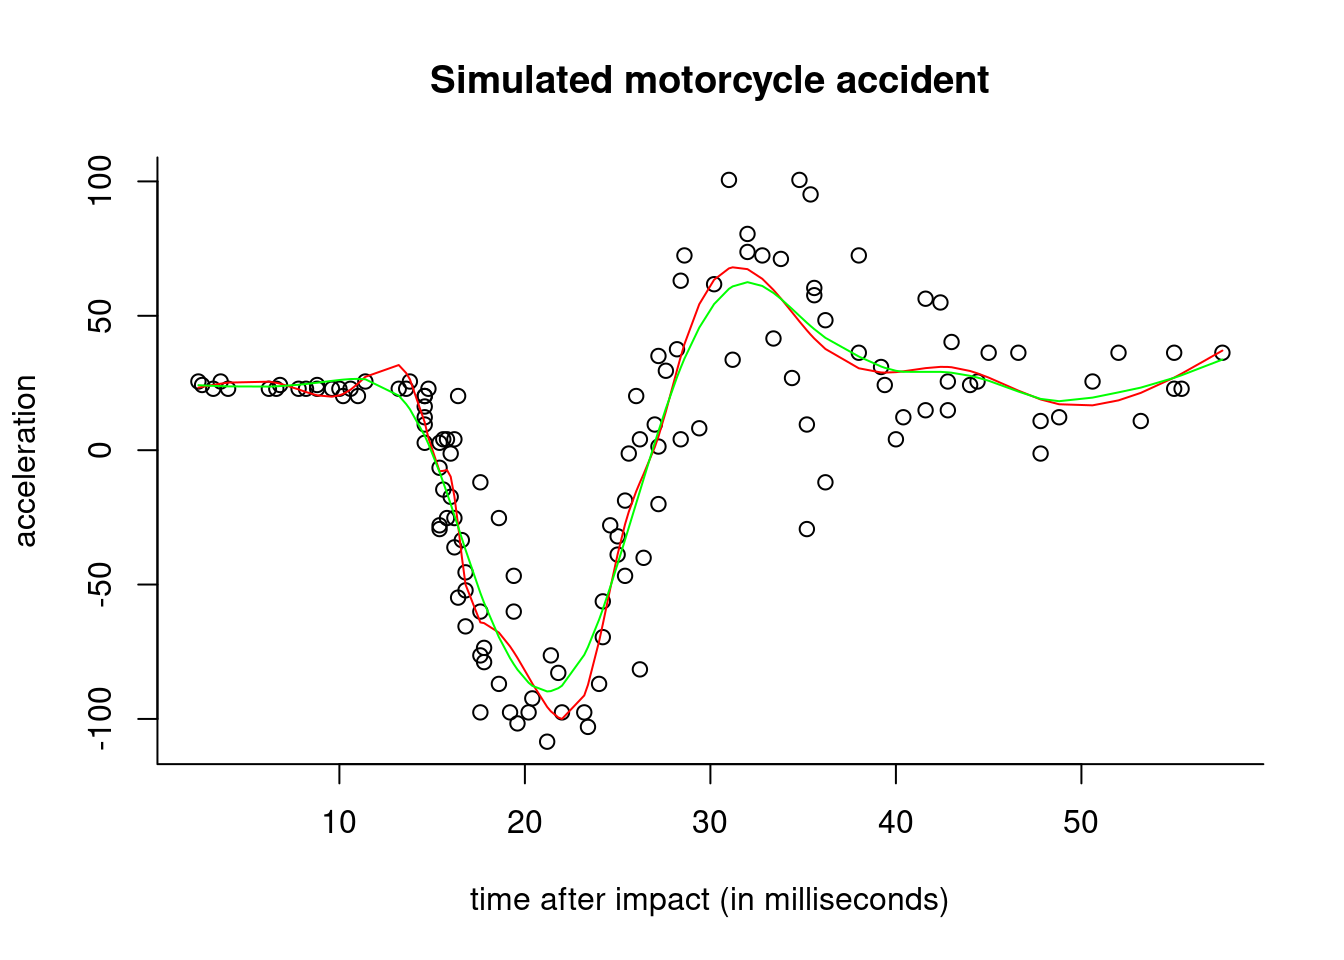
\includegraphics[width=0.7\linewidth]{LineaRModels_files/figure-latex/spline example-1} \end{center}

The fit from the regression spline differs from that of the smoothing spline. The former uses only 18 basis functions and therefore can be fitted using \texttt{lm}, whereas the smoothing spline uses 94 basis functions (this is lower than \(n\) because there are ties in the \texttt{x} vector).

Below is sample code to obtain the \(\mathbf{B}\) and \(\boldsymbol{\Omega}\) matrices, corresponding to the basis functions and the associated penalty.

\begin{Shaded}
\begin{Highlighting}[]
\CommentTok{# You need the fda package installed}
\CommentTok{# install.packages("fda")}
\CommentTok{# Function returns B and Omega matrices}
\NormalTok{smoothsplineb <-}\StringTok{ }\ControlFlowTok{function}\NormalTok{(x)\{}
  \KeywordTok{require}\NormalTok{(fda)}
\NormalTok{  breaks <-}\StringTok{ }\KeywordTok{sort}\NormalTok{(}\KeywordTok{unique}\NormalTok{(x))}
\NormalTok{  basisfd <-}\StringTok{ }\KeywordTok{create.bspline.basis}\NormalTok{(}\DataTypeTok{norder =} \DecValTok{4}\NormalTok{, }\DataTypeTok{breaks =}\NormalTok{ breaks)}
\NormalTok{  B <-}\StringTok{ }\KeywordTok{bsplineS}\NormalTok{(x, }\DataTypeTok{breaks =}\NormalTok{ breaks, }\DataTypeTok{norder =} \DecValTok{4}\NormalTok{, }\DataTypeTok{nderiv =} \DecValTok{0}\NormalTok{)}
\NormalTok{  penmat <-}\StringTok{ }\KeywordTok{bsplinepen}\NormalTok{(basisfd, }\DataTypeTok{Lfd =} \DecValTok{2}\NormalTok{)}
  \KeywordTok{list}\NormalTok{(}\DataTypeTok{basis =}\NormalTok{ B, }\DataTypeTok{penmat =}\NormalTok{ penmat)}
\NormalTok{\}}

\CommentTok{# Compute ridge regression coefficients manually}
\NormalTok{lmridge <-}\StringTok{ }\ControlFlowTok{function}\NormalTok{(y, X, }\DataTypeTok{O =} \KeywordTok{diag}\NormalTok{(}\KeywordTok{length}\NormalTok{(y)), lambda)\{ }
  \KeywordTok{as.vector}\NormalTok{(}\KeywordTok{solve}\NormalTok{(}\KeywordTok{crossprod}\NormalTok{(X) }\OperatorTok{+}\StringTok{ }\NormalTok{lambda}\OperatorTok{*}\NormalTok{O, }\KeywordTok{crossprod}\NormalTok{(X, y)))}
\NormalTok{\}}
\end{Highlighting}
\end{Shaded}

For the \texttt{mcycle} data, the following lines of code return those matrices.

\begin{Shaded}
\begin{Highlighting}[]
\NormalTok{smoothspline_mcycle <-}\StringTok{ }\KeywordTok{smoothsplineb}\NormalTok{(}\DataTypeTok{x =}\NormalTok{ x)}
\NormalTok{B <-}\StringTok{ }\NormalTok{smoothspline_mcycle}\OperatorTok{$}\NormalTok{basis}
\NormalTok{O <-}\StringTok{ }\NormalTok{smoothspline_mcycle}\OperatorTok{$}\NormalTok{penmat}
\end{Highlighting}
\end{Shaded}

\hypertarget{solutions-5}{%
\section{Solutions}\label{solutions-5}}

\hypertarget{exercise-12.4-smoothing-splines}{%
\subsection{Exercise 12.4 Smoothing splines}\label{exercise-12.4-smoothing-splines}}

\begin{Shaded}
\begin{Highlighting}[]
\CommentTok{# Evaluate GCV at a grid of lambda}
\NormalTok{lambdas <-}\StringTok{ }\KeywordTok{seq}\NormalTok{(}\FloatTok{0.1}\NormalTok{, }\DecValTok{40}\NormalTok{, }\DataTypeTok{length =}\NormalTok{ 250L)}
\CommentTok{# Container for GCV criterion}
\NormalTok{gcv <-}\StringTok{ }\KeywordTok{rep}\NormalTok{(}\DecValTok{0}\NormalTok{, }\KeywordTok{length}\NormalTok{(lambdas))  }
\CommentTok{# Loop over cases}
\ControlFlowTok{for}\NormalTok{(i }\ControlFlowTok{in} \DecValTok{1}\OperatorTok{:}\KeywordTok{length}\NormalTok{(lambdas))\{}
  \CommentTok{# Compute smoothing matrix}
\NormalTok{  Sm <-}\StringTok{ }\NormalTok{B }\OperatorTok\StringTok{ }\KeywordTok{solve}\NormalTok{(}\KeywordTok{crossprod}\NormalTok{(B) }\OperatorTok{+}\StringTok{ }\NormalTok{lambdas[i]}\OperatorTok{*}\NormalTok{O) }\OperatorTok\StringTok{ }\KeywordTok{t}\NormalTok{(B)}
  \CommentTok{# Compute ridge regression coefficients}
\NormalTok{  coefs <-}\StringTok{ }\KeywordTok{lmridge}\NormalTok{(}\DataTypeTok{y =}\NormalTok{ y, }\DataTypeTok{X =}\NormalTok{ B, }\DataTypeTok{O =}\NormalTok{ O, }\DataTypeTok{lambda =}\NormalTok{ lambdas[i])}
  \CommentTok{# Compute GCV criterion}
\NormalTok{  gcv[i] <-}\StringTok{ }\KeywordTok{c}\NormalTok{(}\KeywordTok{crossprod}\NormalTok{(y }\OperatorTok{-}\StringTok{ }\NormalTok{B }\OperatorTok\StringTok{ }\NormalTok{coefs)}\OperatorTok{/}\NormalTok{(}\DecValTok{1}\OperatorTok{-}\KeywordTok{mean}\NormalTok{(}\KeywordTok{diag}\NormalTok{(Sm))))}\OperatorTok{/}\KeywordTok{nrow}\NormalTok{(B)}
\NormalTok{\}}
\CommentTok{# Plot GCV}
\KeywordTok{plot}\NormalTok{(lambdas, gcv, }\DataTypeTok{type =} \StringTok{"l"}\NormalTok{, }\DataTypeTok{xlab =} \KeywordTok{expression}\NormalTok{(lambda), }
     \DataTypeTok{ylab =} \StringTok{"GCV criterion value"}\NormalTok{, }\DataTypeTok{main =} \StringTok{"Cross validation"}\NormalTok{)}
\KeywordTok{abline}\NormalTok{(}\DataTypeTok{v =}\NormalTok{ lambdas[}\KeywordTok{which.min}\NormalTok{(gcv)])}
\end{Highlighting}
\end{Shaded}

\begin{center}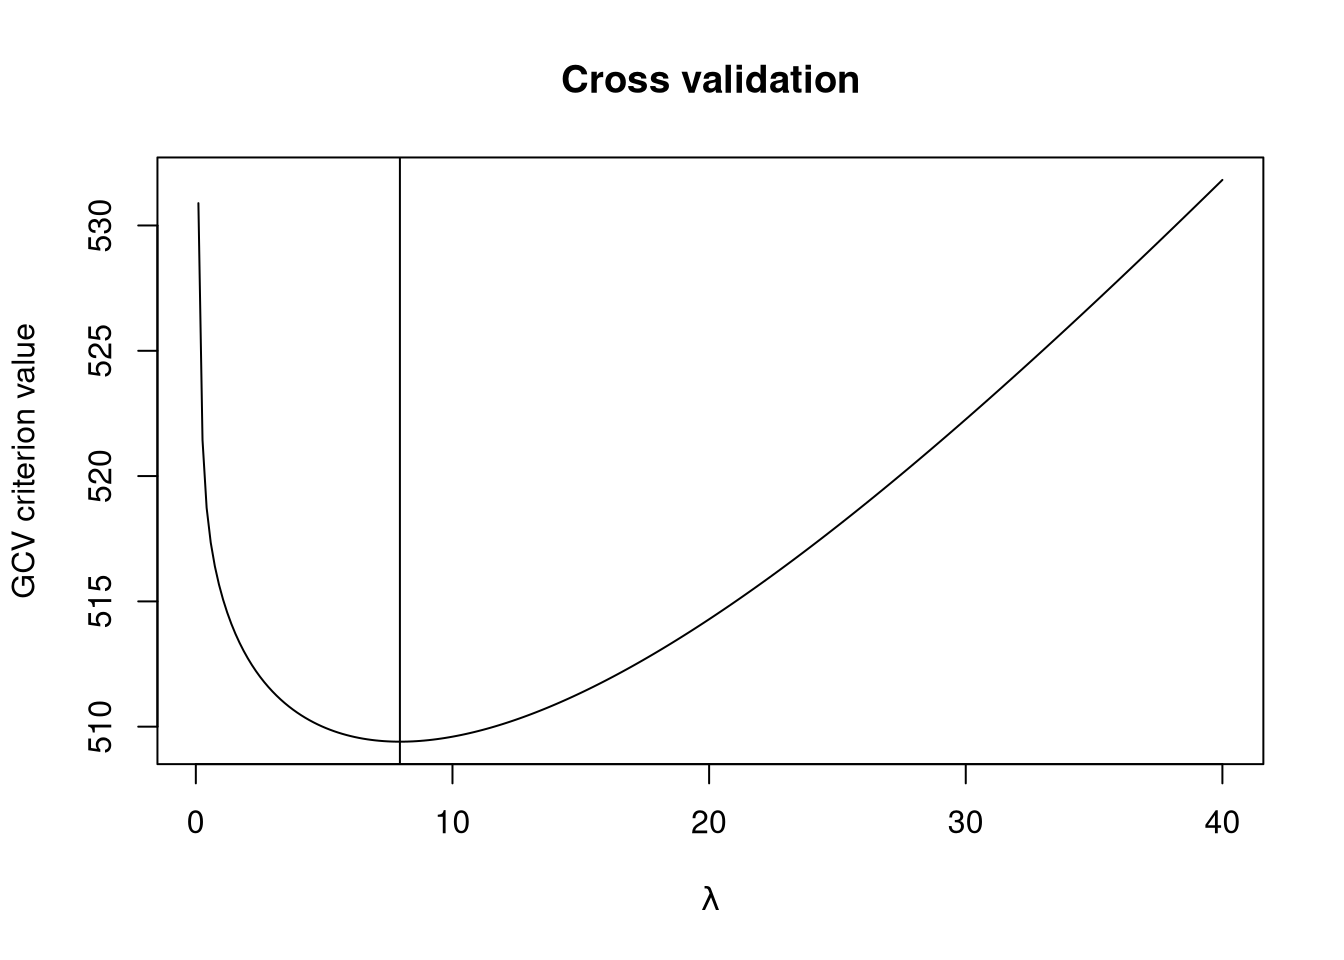
\includegraphics[width=0.7\linewidth]{LineaRModels_files/figure-latex/soln12_4-1} \end{center}

\begin{Shaded}
\begin{Highlighting}[]
\CommentTok{# Plot data}
\KeywordTok{plot}\NormalTok{(y }\OperatorTok{~}\StringTok{ }\NormalTok{x, }\DataTypeTok{xlab =} \StringTok{"time after impact (in milliseconds)"}\NormalTok{, }\DataTypeTok{ylab =} \StringTok{"centered acceleration"}\NormalTok{,}
     \DataTypeTok{main =} \StringTok{"Simulated motorcycle accident"}\NormalTok{, }\DataTypeTok{bty =} \StringTok{"l"}\NormalTok{)}
\CommentTok{# Undersmoothing}
\CommentTok{#lines(x, B %*% lmridge(y = y, X = B, O = O, lambda = 0.01), col = "green")}
\CommentTok{# Oversmoothing}
\CommentTok{#lines(x, B %*% lmridge(y = y, X = B, O = O, lambda = 500), col = "blue")}
\KeywordTok{lines}\NormalTok{(}\KeywordTok{predict}\NormalTok{(}\KeywordTok{smooth.spline}\NormalTok{(}\DataTypeTok{y =}\NormalTok{ y, }\DataTypeTok{x =}\NormalTok{ x, }\DataTypeTok{all.knots =} \OtherTok{TRUE}\NormalTok{)))}
\NormalTok{fitted_opt <-}\StringTok{ }\NormalTok{B }\OperatorTok\StringTok{ }\KeywordTok{lmridge}\NormalTok{(}\DataTypeTok{y =}\NormalTok{ y, }\DataTypeTok{X =}\NormalTok{ B, }\DataTypeTok{O =}\NormalTok{ O,}
                    \DataTypeTok{lambda =}\NormalTok{ lambdas[}\KeywordTok{which.min}\NormalTok{(gcv)])}
\KeywordTok{lines}\NormalTok{(x, fitted_opt , }\DataTypeTok{col =} \StringTok{"red"}\NormalTok{, }\DataTypeTok{lwd =} \DecValTok{2}\NormalTok{)}
\end{Highlighting}
\end{Shaded}

\begin{center}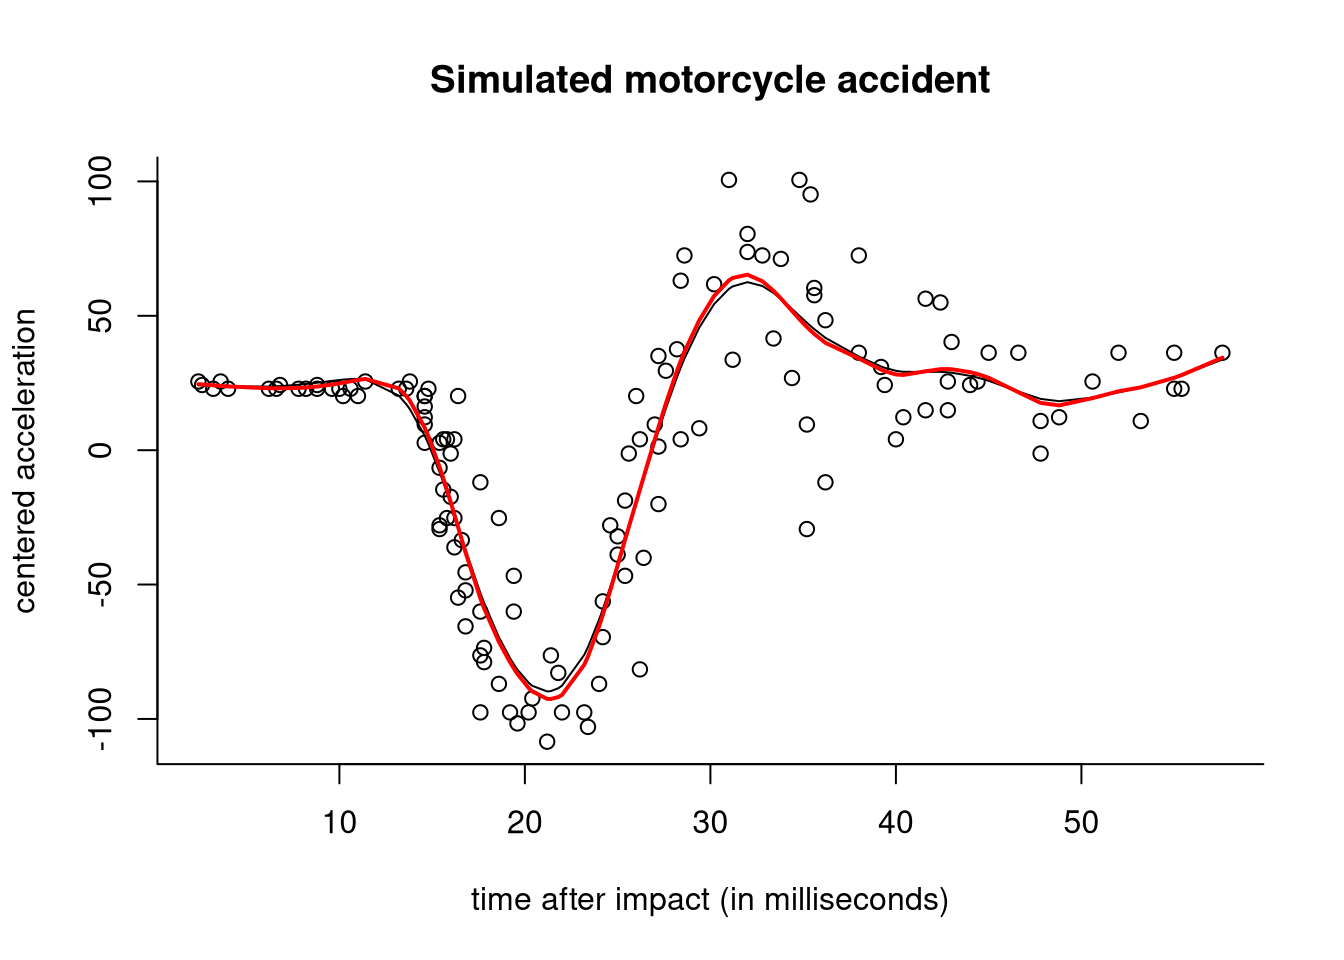
\includegraphics[width=0.7\linewidth]{LineaRModels_files/figure-latex/soln12_4-2} \end{center}

\hypertarget{generalized-linear-models}{%
\chapter{Generalized linear models}\label{generalized-linear-models}}

In class, we have covered basic of generalized linear models (GLM), including binary and binomial models with logistic link function and the Poisson regression model with log link. The unifying theory behind GLM will be covered in MATH 408. The goal of this tutorial is to give you additional examples on how to fit these models.

Outside of parameter estimation (which proceeds through Fisher scoring in R), we will look at analysis of deviance (a likelihood ratio test for testing whether coefficients are zero, resulting in a comparison between two nested models). We proceed with the latter in exactly the same way as for analysis of variance, modulo the fact that we use the \(\chi^2\) asymptotic distribution in place of the Fisher \(F\) distribution. Similarly, the \(P\)-values for the Wald tests are based on the asymptotic distribution of the test, which is Gaussian.

The specification of the GLM object in \textbf{R} is analogous to the one for an \texttt{lm} object.
We use \texttt{y\ \textasciitilde{}\ x} formula syntax to specify the mean relationship. If you have a binomial data, the response should be a two column matrix with integer elements \((k_i, n_i-k_i)\) specifying the number of successes and failures, respectively, for each case or cell.

The second difference between \texttt{lm} and \texttt{glm} is the presence of the argument \texttt{family} that allow you to specify the likelihood

\begin{itemize}
\tightlist
\item
  \texttt{family\ =\ gaussian()} gives back a linear model;
\item
  \texttt{family\ =\ binomial("logit")} gives you a binary or binomial regression with logistic link function;
\item
  \texttt{family\ =\ poisson()} gives you Poisson regression.
\end{itemize}

By default, empty parenthesis give the so-called canonical link function (identity for normal, logit for binomial and log for Poisson).

Let \(\ell\) denote the log-likelihood function for an \(n\) sample. The function \texttt{glm} uses Fisher scoring to obtain the maximum likelihood estimates, based on the recursion
\[ \boldsymbol{\beta}^{(t+1)} = \boldsymbol{\beta}^{(t)} + \mathcal{I}^{-1}_n(\boldsymbol{\beta}^{(t)}) \left. \frac{\partial \ell}{\partial \boldsymbol{\beta}} \right|_{\boldsymbol{\beta}=\boldsymbol{\beta}^{(t)} },\]
where the Fisher information
\[\mathcal{I}_n =\mathrm{E}\left(  \frac{\partial \ell}{\partial \boldsymbol{\beta}}\frac{\partial \ell}{\partial \boldsymbol{\beta}^\top}\right)\]
is estimated at the current value of \(\boldsymbol{\beta}^{(t)}\). The IRLS algorithm uses the observed information.

\hypertarget{diagnostics-for-bernoulli-data}{%
\section{Diagnostics for Bernoulli data}\label{diagnostics-for-bernoulli-data}}

This is the example presented in class. The response variable is a binary indicator of low birthweight.

\begin{Shaded}
\begin{Highlighting}[]
\KeywordTok{data}\NormalTok{(birthwt, }\DataTypeTok{package =} \StringTok{"MASS"}\NormalTok{)}
\CommentTok{# Preprocessing from MASS - give meaningful labels for factors}
\CommentTok{# See help for description of the data set}
\CommentTok{# Rewrite a new data frame with those variables}
\NormalTok{bwt <-}\StringTok{ }\KeywordTok{with}\NormalTok{(birthwt, \{}
\NormalTok{  race <-}\StringTok{ }\KeywordTok{factor}\NormalTok{(race, }\DataTypeTok{labels =} \KeywordTok{c}\NormalTok{(}\StringTok{"white"}\NormalTok{, }\StringTok{"black"}\NormalTok{, }\StringTok{"other"}\NormalTok{))}
\NormalTok{  ptd <-}\StringTok{ }\KeywordTok{factor}\NormalTok{(ptl }\OperatorTok{>}\StringTok{ }\DecValTok{0}\NormalTok{)}
\NormalTok{  ftv <-}\StringTok{ }\KeywordTok{factor}\NormalTok{(ftv) }
  \CommentTok{# Group number of visits to avoid categories with small counts}
  \KeywordTok{levels}\NormalTok{(ftv)[}\OperatorTok{-}\NormalTok{(}\DecValTok{1}\OperatorTok{:}\DecValTok{2}\NormalTok{)] <-}\StringTok{ "2+"}
  \KeywordTok{data.frame}\NormalTok{(}\DataTypeTok{low =} \KeywordTok{factor}\NormalTok{(low), age, lwt, race, }\DataTypeTok{smoke =}\NormalTok{ (smoke }\OperatorTok{>}\StringTok{ }\DecValTok{0}\NormalTok{),}
\NormalTok{             ptd, }\DataTypeTok{ht =}\NormalTok{ (ht }\OperatorTok{>}\StringTok{ }\DecValTok{0}\NormalTok{), }\DataTypeTok{ui =}\NormalTok{ (ui }\OperatorTok{>}\StringTok{ }\DecValTok{0}\NormalTok{), ftv)}
\NormalTok{  \})}

\NormalTok{lbw <-}\StringTok{ }\KeywordTok{glm}\NormalTok{(low }\OperatorTok{~}\StringTok{ }\NormalTok{., }\DataTypeTok{family =}\NormalTok{ binomial, }\DataTypeTok{data =}\NormalTok{ bwt)}
\CommentTok{# Can use summary just like for lm}
\KeywordTok{summary}\NormalTok{(lbw)}
\end{Highlighting}
\end{Shaded}

\begin{verbatim}
## 
## Call:
## glm(formula = low ~ ., family = binomial, data = bwt)
## 
## Deviance Residuals: 
##     Min       1Q   Median       3Q      Max  
## -1.7038  -0.8068  -0.5008   0.8835   2.2152  
## 
## Coefficients:
##             Estimate Std. Error z value Pr(>|z|)
## (Intercept)  0.82302    1.24471   0.661  0.50848
## age         -0.03723    0.03870  -0.962  0.33602
## lwt         -0.01565    0.00708  -2.211  0.02705
## raceblack    1.19241    0.53597   2.225  0.02609
## raceother    0.74069    0.46174   1.604  0.10869
## smokeTRUE    0.75553    0.42502   1.778  0.07546
## ptdTRUE      1.34376    0.48062   2.796  0.00518
## htTRUE       1.91317    0.72074   2.654  0.00794
## uiTRUE       0.68019    0.46434   1.465  0.14296
## ftv1        -0.43638    0.47939  -0.910  0.36268
## ftv2+        0.17901    0.45638   0.392  0.69488
## 
## (Dispersion parameter for binomial family taken to be 1)
## 
##     Null deviance: 234.67  on 188  degrees of freedom
## Residual deviance: 195.48  on 178  degrees of freedom
## AIC: 217.48
## 
## Number of Fisher Scoring iterations: 4
\end{verbatim}

The \texttt{summary} object returns the coefficients, standard errors and results for the Wald test that \(\beta_i=0\). Note that these will generally differ from the likelihood ratio test.
The code above illustrates how to fit the Bernoulli model. Since the data are binary, there is no need to give two columns as response. The following code produces diagnostics for the model as shown in class:

\begin{Shaded}
\begin{Highlighting}[]
\NormalTok{binmod <-}\StringTok{ }\KeywordTok{glm}\NormalTok{(}\DataTypeTok{formula =}\NormalTok{ low }\OperatorTok{~}\StringTok{ }\NormalTok{lwt }\OperatorTok{+}\StringTok{ }\NormalTok{race }\OperatorTok{+}\StringTok{ }\NormalTok{smoke }\OperatorTok{+}\StringTok{ }\NormalTok{ptd }\OperatorTok{+}\StringTok{ }\NormalTok{ht }\OperatorTok{+}\StringTok{ }\NormalTok{ui, }
           \DataTypeTok{family =} \KeywordTok{binomial}\NormalTok{(}\DataTypeTok{link =} \StringTok{"logit"}\NormalTok{), }\DataTypeTok{data =}\NormalTok{ bwt)}
\CommentTok{#Logit link function}
\NormalTok{logit <-}\StringTok{ }\ControlFlowTok{function}\NormalTok{(x)\{}\KeywordTok{log}\NormalTok{(x)}\OperatorTok{-}\KeywordTok{log}\NormalTok{(}\DecValTok{1}\OperatorTok{-}\NormalTok{x)\}}
\NormalTok{n <-}\StringTok{ }\KeywordTok{length}\NormalTok{(}\KeywordTok{fitted}\NormalTok{(binmod))}
\NormalTok{U1 <-}\StringTok{ }\KeywordTok{runif}\NormalTok{(n, }\DataTypeTok{min =} \DecValTok{0}\NormalTok{, }\DataTypeTok{max =} \KeywordTok{fitted}\NormalTok{(binmod))}
\NormalTok{U2 <-}\StringTok{ }\KeywordTok{runif}\NormalTok{(n, }\DataTypeTok{min =} \KeywordTok{fitted}\NormalTok{(binmod), }\DataTypeTok{max =} \DecValTok{1}\NormalTok{)}
\NormalTok{unires <-}\StringTok{ }\NormalTok{binmod}\OperatorTok{$}\NormalTok{y}\OperatorTok{*}\NormalTok{U1 }\OperatorTok{+}\StringTok{ }\NormalTok{U2}\OperatorTok{*}\NormalTok{(}\DecValTok{1}\OperatorTok{-}\NormalTok{binmod}\OperatorTok{$}\NormalTok{y)}
\KeywordTok{par}\NormalTok{(}\DataTypeTok{pty =} \StringTok{"s"}\NormalTok{, }\DataTypeTok{mfrow =} \KeywordTok{c}\NormalTok{(}\DecValTok{2}\NormalTok{, }\DecValTok{2}\NormalTok{), }\DataTypeTok{bty =} \StringTok{"l"}\NormalTok{, }\DataTypeTok{pch =} \DecValTok{20}\NormalTok{)}
\KeywordTok{plot}\NormalTok{(bwt}\OperatorTok{$}\NormalTok{lwt, unires, }\DataTypeTok{ylab =} \StringTok{"uniform residuals"}\NormalTok{,}
     \DataTypeTok{xlab =} \StringTok{"mother's weight (in pounds)"}\NormalTok{)}
\KeywordTok{plot}\NormalTok{(}\KeywordTok{logit}\NormalTok{(}\KeywordTok{fitted}\NormalTok{(binmod)), unires, }\DataTypeTok{ylab =} \StringTok{"uniform residuals"}\NormalTok{,}
     \DataTypeTok{xlab =} \StringTok{"logit(p)"}\NormalTok{)}
\KeywordTok{hist}\NormalTok{(unires, }\DataTypeTok{probability =} \OtherTok{TRUE}\NormalTok{, }\DataTypeTok{main =} \StringTok{""}\NormalTok{, }\DataTypeTok{xlab =} \StringTok{"uniform residuals"}\NormalTok{)}

\CommentTok{# Quantile - quantile plot}
\KeywordTok{plot}\NormalTok{(}\DataTypeTok{x =} \KeywordTok{rank}\NormalTok{(unires)}\OperatorTok{/}\NormalTok{(n }\OperatorTok{+}\StringTok{ }\DecValTok{1}\NormalTok{), }\DataTypeTok{y =}\NormalTok{ unires, }
     \DataTypeTok{xlab =} \StringTok{"Theoretical quantiles"}\NormalTok{, }\DataTypeTok{ylab =} \StringTok{"Observed quantiles"}\NormalTok{, }
     \DataTypeTok{xlim =} \KeywordTok{c}\NormalTok{(}\DecValTok{0}\NormalTok{, }\DecValTok{1}\NormalTok{), }\DataTypeTok{ylim =} \KeywordTok{c}\NormalTok{(}\DecValTok{0}\NormalTok{, }\DecValTok{1}\NormalTok{), }\DataTypeTok{cex =} \FloatTok{0.5}\NormalTok{)}
\KeywordTok{abline}\NormalTok{(}\DataTypeTok{a =} \DecValTok{0}\NormalTok{, }\DataTypeTok{b =} \DecValTok{1}\NormalTok{)}
\CommentTok{# Simulated confidence bands, based on quantiles of the uniform distribution}
\NormalTok{pconfint <-}\StringTok{ }\KeywordTok{apply}\NormalTok{(}\KeywordTok{apply}\NormalTok{(}\KeywordTok{matrix}\NormalTok{(}\KeywordTok{runif}\NormalTok{(}\DecValTok{10000} \OperatorTok{*}\StringTok{ }\NormalTok{n), }\DataTypeTok{nrow =}\NormalTok{ n), }\DecValTok{2}\NormalTok{, sort), }\DecValTok{1}\NormalTok{, quantile, }\DataTypeTok{probs =} \KeywordTok{c}\NormalTok{(}\FloatTok{0.025}\NormalTok{, }\FloatTok{0.975}\NormalTok{))}
\KeywordTok{lines}\NormalTok{((}\DecValTok{1}\OperatorTok{:}\NormalTok{n)}\OperatorTok{/}\NormalTok{(n}\OperatorTok{+}\DecValTok{1}\NormalTok{), pconfint[}\DecValTok{1}\NormalTok{,], }\DataTypeTok{lty =} \DecValTok{2}\NormalTok{, }\DataTypeTok{col =} \DecValTok{2}\NormalTok{)}
\KeywordTok{lines}\NormalTok{((}\DecValTok{1}\OperatorTok{:}\NormalTok{n)}\OperatorTok{/}\NormalTok{(n}\OperatorTok{+}\DecValTok{1}\NormalTok{), pconfint[}\DecValTok{2}\NormalTok{,], }\DataTypeTok{lty =} \DecValTok{2}\NormalTok{, }\DataTypeTok{col =} \DecValTok{2}\NormalTok{)}
\end{Highlighting}
\end{Shaded}

\begin{center}\includegraphics[width=0.7\linewidth]{LineaRModels_files/figure-latex/glmdiag-1} \end{center}

\hypertarget{poisson-model-for-contingency-table}{%
\section{Poisson model for contingency table}\label{poisson-model-for-contingency-table}}

We analyze a \(4 \times 3\) contingency table containing information about tumour type.
The first factor is cancer \texttt{type}, with levels

\begin{enumerate}
\def\labelenumi{\arabic{enumi}.}
\tightlist
\item
  Hutchinson's melanotic freckle,
\item
  Superficial spreading melanoma,
\item
  Nodular
\item
  for Indeterminate type
\end{enumerate}

The second variable, \texttt{site}, is one of
1. Head and Neck,
2. Trunk,
3. Extremities

The data are count, hence we proceed with the analysis using a Poisson likelihood. This ressembles ANOVA models with factors.

\begin{Shaded}
\begin{Highlighting}[]
\CommentTok{# Create dataset}
\NormalTok{site <-}\StringTok{ }\KeywordTok{gl}\NormalTok{(}\DataTypeTok{n =} \DecValTok{3}\NormalTok{, }\DataTypeTok{k =} \DecValTok{1}\NormalTok{, }\DataTypeTok{length =} \DecValTok{12}\NormalTok{) }
\CommentTok{# gl generates levels of a factor}
\NormalTok{tumor <-}\StringTok{ }\KeywordTok{gl}\NormalTok{(}\DataTypeTok{n =} \DecValTok{4}\NormalTok{, }\DataTypeTok{k =} \DecValTok{3}\NormalTok{) }\CommentTok{#each 3}
\NormalTok{cases <-}\StringTok{ }\KeywordTok{c}\NormalTok{(}\DecValTok{22}\NormalTok{, }\DecValTok{2}\NormalTok{, }\DecValTok{10}\NormalTok{, }\DecValTok{16}\NormalTok{, }\DecValTok{54}\NormalTok{, }\DecValTok{115}\NormalTok{, }\DecValTok{19}\NormalTok{, }\DecValTok{33}\NormalTok{, }\DecValTok{73}\NormalTok{, }\DecValTok{11}\NormalTok{, }\DecValTok{17}\NormalTok{, }\DecValTok{28}\NormalTok{)}
\NormalTok{cancer <-}\StringTok{ }\KeywordTok{data.frame}\NormalTok{(tumor, site, cases)}
\CommentTok{# Four cases - no effect, main interaction only, additive}
\NormalTok{cancer.m0 <-}\StringTok{ }\KeywordTok{glm}\NormalTok{(cases }\OperatorTok{~}\StringTok{ }\DecValTok{1}\NormalTok{, }\DataTypeTok{family =}\NormalTok{ poisson, }\DataTypeTok{data =}\NormalTok{ cancer)}
\NormalTok{cancer.m1 <-}\StringTok{ }\KeywordTok{glm}\NormalTok{(cases }\OperatorTok{~}\StringTok{ }\NormalTok{tumor, }\DataTypeTok{family =}\NormalTok{ poisson, }\DataTypeTok{data =}\NormalTok{ cancer)}
\NormalTok{cancer.m2 <-}\StringTok{ }\KeywordTok{glm}\NormalTok{(cases }\OperatorTok{~}\StringTok{ }\NormalTok{site, }\DataTypeTok{family =}\NormalTok{ poisson, }\DataTypeTok{data =}\NormalTok{ cancer)}
\NormalTok{cancer.m3 <-}\StringTok{ }\KeywordTok{glm}\NormalTok{(cases }\OperatorTok{~}\StringTok{ }\NormalTok{tumor }\OperatorTok{+}\StringTok{ }\NormalTok{site, }\DataTypeTok{family =}\NormalTok{ poisson, }\DataTypeTok{data =}\NormalTok{ cancer)}
\CommentTok{# Saturated model}
\NormalTok{cancer.m4 <-}\StringTok{ }\KeywordTok{glm}\NormalTok{(cases }\OperatorTok{~}\StringTok{ }\NormalTok{tumor }\OperatorTok{*}\StringTok{ }\NormalTok{site, }\DataTypeTok{family =}\NormalTok{ poisson, }\DataTypeTok{data =}\NormalTok{ cancer)}
\CommentTok{# Analysis of deviance}
\CommentTok{# Same syntax as for GLM}
\KeywordTok{drop1}\NormalTok{(cancer.m4)}
\end{Highlighting}
\end{Shaded}

\begin{verbatim}
## Single term deletions
## 
## Model:
## cases ~ tumor * site
##            Df Deviance     AIC
## <none>           0.000  83.111
## tumor:site  6   51.795 122.906
\end{verbatim}

\begin{Shaded}
\begin{Highlighting}[]
\KeywordTok{anova}\NormalTok{(cancer.m3, cancer.m4, }\DataTypeTok{test =} \StringTok{"Chisq"}\NormalTok{)}
\end{Highlighting}
\end{Shaded}

\begin{verbatim}
## Analysis of Deviance Table
## 
## Model 1: cases ~ tumor + site
## Model 2: cases ~ tumor * site
##   Resid. Df Resid. Dev Df Deviance      Pr(>Chi)
## 1         6     51.795                          
## 2         0      0.000  6   51.795 0.00000000205
\end{verbatim}

\begin{Shaded}
\begin{Highlighting}[]
\CommentTok{# anova(cancer.m4) returns three tests, }
\CommentTok{# but only the comparison with additive model is justified}
\KeywordTok{summary}\NormalTok{(cancer.m4)}
\end{Highlighting}
\end{Shaded}

\begin{verbatim}
## 
## Call:
## glm(formula = cases ~ tumor * site, family = poisson, data = cancer)
## 
## Deviance Residuals: 
##  [1]  0  0  0  0  0  0  0  0  0  0  0  0
## 
## Coefficients:
##              Estimate Std. Error z value    Pr(>|z|)
## (Intercept)    3.0910     0.2132  14.498     < 2e-16
## tumor2        -0.3185     0.3286  -0.969    0.332432
## tumor3        -0.1466     0.3132  -0.468    0.639712
## tumor4        -0.6931     0.3693  -1.877    0.060511
## site2         -2.3979     0.7385  -3.247    0.001167
## site3         -0.7885     0.3814  -2.067    0.038701
## tumor2:site2   3.6143     0.7915   4.566 0.000004962
## tumor3:site2   2.9500     0.7927   3.721    0.000198
## tumor4:site2   2.8332     0.8338   3.398    0.000679
## tumor2:site3   2.7608     0.4655   5.931 0.000000003
## tumor3:site3   2.1345     0.4602   4.638 0.000003516
## tumor4:site3   1.7228     0.5216   3.303    0.000957
## 
## (Dispersion parameter for poisson family taken to be 1)
## 
##     Null deviance: 2.9520e+02  on 11  degrees of freedom
## Residual deviance: 7.9936e-15  on  0  degrees of freedom
## AIC: 83.111
## 
## Number of Fisher Scoring iterations: 3
\end{verbatim}

\begin{Shaded}
\begin{Highlighting}[]
\CommentTok{# Alternatively, compute manually}
\DecValTok{1} \OperatorTok{-}\StringTok{ }\KeywordTok{pchisq}\NormalTok{(}\KeywordTok{deviance}\NormalTok{(cancer.m3), }\DataTypeTok{df =}\NormalTok{ cancer.m3}\OperatorTok{$}\NormalTok{df.residual)}
\end{Highlighting}
\end{Shaded}

\begin{verbatim}
## [1] 0.000000002050453
\end{verbatim}

The likelihood ratio test to check whether the interaction is significative is soundly rejected, hence we would keep the saturated model. For such a model, the fitted values correspond to the observed counts.

This is an example where the hypothesis of equal mean and variance does not seem to hold. Handling the overdispersion is beyond the scope of this course.

\hypertarget{solutions-6}{%
\section{Solutions}\label{solutions-6}}

\hypertarget{exercise-13.3---two-way-contingency-tables}{%
\subsection{Exercise 13.3 - Two-way contingency tables}\label{exercise-13.3---two-way-contingency-tables}}

\begin{Shaded}
\begin{Highlighting}[]
\NormalTok{cancer <-}\StringTok{ }\KeywordTok{read.table}\NormalTok{(}\StringTok{"https://lbelzile.bitbucket.io/math341/cancer.dat"}\NormalTok{, }\DataTypeTok{header =} \OtherTok{TRUE}\NormalTok{)}
\KeywordTok{print}\NormalTok{(cancer)}
\end{Highlighting}
\end{Shaded}

\begin{verbatim}
##      age malignant yes no
## 1    <50       yes  26  9
## 2    <50        no  68  7
## 3    <50       yes  25  4
## 4    <50        no   9  3
## 5  50-69       yes  20  9
## 6  50-69        no  46  9
## 7  50-69       yes  18 11
## 8  50-69        no   5  2
## 9    70+       yes   1  2
## 10   70+        no   6  3
## 11   70+       yes   5  1
## 12   70+        no   1  0
## 13   <50       yes  11  6
## 14   <50        no  24  7
## 15   <50       yes   4  6
## 16   <50        no   0  0
## 17 50-69       yes  18  8
## 18 50-69        no  58 20
## 19 50-69       yes  10  3
## 20 50-69        no   3  2
## 21   70+       yes  15  9
## 22   70+        no  26 18
## 23   70+       yes   1  3
## 24   70+        no   1  0
## 25   <50       yes  16 16
## 26   <50        no  20  7
## 27   <50       yes   8  3
## 28   <50        no   1  0
## 29 50-69       yes  27 14
## 30 50-69        no  39 12
## 31 50-69       yes  10  3
## 32 50-69        no   4  0
## 33   70+       yes  12  3
## 34   70+        no  11  7
## 35   70+       yes   4  3
## 36   70+        no   1  0
\end{verbatim}

\begin{Shaded}
\begin{Highlighting}[]
\CommentTok{# Some categories have small counts, so asymptotic result may be a bit off}

\NormalTok{cancer.m0 <-}\StringTok{ }\KeywordTok{glm}\NormalTok{(}\KeywordTok{cbind}\NormalTok{(yes, no) }\OperatorTok{~}\StringTok{ }\DecValTok{1}\NormalTok{, }\DataTypeTok{family =} \StringTok{"binomial"}\NormalTok{, }\DataTypeTok{data =}\NormalTok{ cancer)}
\NormalTok{cancer.m1 <-}\StringTok{ }\KeywordTok{glm}\NormalTok{(}\KeywordTok{cbind}\NormalTok{(yes, no) }\OperatorTok{~}\StringTok{ }\NormalTok{age, }\DataTypeTok{family =} \StringTok{"binomial"}\NormalTok{, }\DataTypeTok{data =}\NormalTok{ cancer)}
\NormalTok{cancer.m2 <-}\StringTok{ }\KeywordTok{glm}\NormalTok{(}\KeywordTok{cbind}\NormalTok{(yes, no) }\OperatorTok{~}\StringTok{ }\NormalTok{malignant, }\DataTypeTok{family =} \StringTok{"binomial"}\NormalTok{, }\DataTypeTok{data =}\NormalTok{ cancer)}
\NormalTok{cancer.m3 <-}\StringTok{ }\KeywordTok{glm}\NormalTok{(}\KeywordTok{cbind}\NormalTok{(yes, no) }\OperatorTok{~}\StringTok{ }\NormalTok{age }\OperatorTok{+}\StringTok{ }\NormalTok{malignant, }\DataTypeTok{family =} \StringTok{"binomial"}\NormalTok{, }\DataTypeTok{data =}\NormalTok{ cancer)}
\NormalTok{cancer.m4 <-}\StringTok{ }\KeywordTok{glm}\NormalTok{(}\KeywordTok{cbind}\NormalTok{(yes, no) }\OperatorTok{~}\StringTok{ }\NormalTok{age }\OperatorTok{*}\StringTok{ }\NormalTok{malignant, }\DataTypeTok{family =} \StringTok{"binomial"}\NormalTok{, }\DataTypeTok{data =}\NormalTok{ cancer)}
\KeywordTok{library}\NormalTok{(xtable)}
\NormalTok{devtab <-}\StringTok{ }\KeywordTok{data.frame}\NormalTok{(}\StringTok{"model"}\NormalTok{ =}\StringTok{ }\KeywordTok{c}\NormalTok{(}\StringTok{"M0"}\NormalTok{,}\StringTok{"M1"}\NormalTok{,}\StringTok{"M2"}\NormalTok{,}\StringTok{"M3"}\NormalTok{), }
                     \StringTok{"deviance"}\NormalTok{ =}\StringTok{ }\KeywordTok{round}\NormalTok{(}\KeywordTok{c}\NormalTok{(}\KeywordTok{deviance}\NormalTok{(cancer.m0), }\KeywordTok{deviance}\NormalTok{(cancer.m1), }
                                          \KeywordTok{deviance}\NormalTok{(cancer.m2), }\KeywordTok{deviance}\NormalTok{(cancer.m3)), }\DecValTok{2}\NormalTok{),}
      \StringTok{"p"}\NormalTok{ =}\StringTok{ }\KeywordTok{c}\NormalTok{(}\KeywordTok{length}\NormalTok{(}\KeywordTok{coef}\NormalTok{(cancer.m0)),}\KeywordTok{length}\NormalTok{(}\KeywordTok{coef}\NormalTok{(cancer.m1)),}
              \KeywordTok{length}\NormalTok{(}\KeywordTok{coef}\NormalTok{(cancer.m2)),}\KeywordTok{length}\NormalTok{(}\KeywordTok{coef}\NormalTok{(cancer.m3))))}

\NormalTok{devtab}
\end{Highlighting}
\end{Shaded}

\begin{verbatim}
##   model deviance p
## 1    M0    57.59 1
## 2    M1    50.44 3
## 3    M2    48.59 2
## 4    M3    41.06 4
\end{verbatim}

Now that we have calculated the deviance of every model, we can perform an analysis of deviance and check
whether the final model obtained by backward elimination is adequate by comparing its \(P\)-value under the null.
Some counts in the age category \texttt{70+} are very low, hence the asymptotic result can be a bit off. We assess this through a small simulation study in which we resample observations from the fitted model.

\begin{Shaded}
\begin{Highlighting}[]
\CommentTok{# Saturated model vs additive model}
 \DecValTok{1}\OperatorTok{-}\StringTok{ }\KeywordTok{pchisq}\NormalTok{(}\KeywordTok{deviance}\NormalTok{(cancer.m3), }\DataTypeTok{df =} \KeywordTok{nrow}\NormalTok{(cancer) }\OperatorTok{-}\StringTok{ }\KeywordTok{length}\NormalTok{(cancer.m3}\OperatorTok{$}\NormalTok{coef))}
\end{Highlighting}
\end{Shaded}

\begin{verbatim}
## [1] 0.7811038
\end{verbatim}

\begin{Shaded}
\begin{Highlighting}[]
\CommentTok{# p-value of 0.78, fail to reject null that additive model is adequate}
\CommentTok{# Try further simplification}
\KeywordTok{drop1}\NormalTok{(cancer.m3, }\DataTypeTok{test =} \StringTok{"Chisq"}\NormalTok{)}
\end{Highlighting}
\end{Shaded}

\begin{verbatim}
## Single term deletions
## 
## Model:
## cbind(yes, no) ~ age + malignant
##           Df Deviance    AIC    LRT Pr(>Chi)
## <none>         0.4941 30.433                
## age        2   5.9552 31.894 5.4611  0.06518
## malignant  1   6.6412 34.580 6.1471  0.01316
\end{verbatim}

\begin{Shaded}
\begin{Highlighting}[]
\CommentTok{# Fail to reject null that model with only "malignant" is adequate simplification}
 \DecValTok{1}\OperatorTok{-}\StringTok{ }\KeywordTok{pchisq}\NormalTok{(}\DecValTok{2}\OperatorTok{*}\NormalTok{(}\KeywordTok{c}\NormalTok{(}\KeywordTok{logLik}\NormalTok{(cancer.m3) }\OperatorTok{-}\StringTok{ }\KeywordTok{logLik}\NormalTok{(cancer.m2))), }\DataTypeTok{df =}\NormalTok{ (}\KeywordTok{length}\NormalTok{(cancer.m3}\OperatorTok{$}\NormalTok{coef) }\OperatorTok{-}\StringTok{ }\KeywordTok{length}\NormalTok{(cancer.m2}\OperatorTok{$}\NormalTok{coef)))}
\end{Highlighting}
\end{Shaded}

\begin{verbatim}
## [1] 0.06518224
\end{verbatim}

\begin{Shaded}
\begin{Highlighting}[]
 \DecValTok{1}\OperatorTok{-}\StringTok{ }\KeywordTok{pchisq}\NormalTok{(}\DecValTok{2}\OperatorTok{*}\NormalTok{(}\KeywordTok{c}\NormalTok{(}\KeywordTok{logLik}\NormalTok{(cancer.m3) }\OperatorTok{-}\StringTok{ }\KeywordTok{logLik}\NormalTok{(cancer.m1))), }\DataTypeTok{df =}\NormalTok{ (}\KeywordTok{length}\NormalTok{(cancer.m3}\OperatorTok{$}\NormalTok{coef) }\OperatorTok{-}\StringTok{ }\KeywordTok{length}\NormalTok{(cancer.m1}\OperatorTok{$}\NormalTok{coef)))}
\end{Highlighting}
\end{Shaded}

\begin{verbatim}
## [1] 0.01316278
\end{verbatim}

\begin{Shaded}
\begin{Highlighting}[]
\KeywordTok{drop1}\NormalTok{(cancer.m2, }\DataTypeTok{test =} \StringTok{"Chisq"}\NormalTok{)}
\end{Highlighting}
\end{Shaded}

\begin{verbatim}
## Single term deletions
## 
## Model:
## cbind(yes, no) ~ malignant
##           Df Deviance    AIC    LRT Pr(>Chi)
## <none>         5.9552 31.894                
## malignant  1  12.6558 36.595 6.7006 0.009638
\end{verbatim}

\begin{Shaded}
\begin{Highlighting}[]
\CommentTok{# Reject null that model with only intercept is adequate}

\CommentTok{# If Model is adequate, Deviance approx JK-p }
\KeywordTok{deviance}\NormalTok{(cancer.m2)}
\end{Highlighting}
\end{Shaded}

\begin{verbatim}
## [1] 5.955231
\end{verbatim}

\begin{Shaded}
\begin{Highlighting}[]
\CommentTok{# Is this result vary large? Investigate via simulation study}
\CommentTok{# Canonical link functions for binomial}
\NormalTok{logit <-}\StringTok{ }\ControlFlowTok{function}\NormalTok{(x)\{}\KeywordTok{log}\NormalTok{(x) }\OperatorTok{-}\StringTok{ }\KeywordTok{log}\NormalTok{(}\DecValTok{1}\OperatorTok{-}\NormalTok{x)\}}
\CommentTok{# Inverse link function (logistic in course notes)}
\NormalTok{expit <-}\StringTok{ }\ControlFlowTok{function}\NormalTok{(x)\{ }\DecValTok{1}\OperatorTok{/}\NormalTok{(}\DecValTok{1}\OperatorTok{+}\StringTok{ }\KeywordTok{exp}\NormalTok{(}\OperatorTok{-}\NormalTok{x))\}}
\CommentTok{# Get predicted probability}
\NormalTok{probc <-}\StringTok{ }\KeywordTok{expit}\NormalTok{(}\KeywordTok{predict}\NormalTok{(cancer.m2))}
\CommentTok{# Need to condition on total count - fixed for binomial model}
\NormalTok{nr <-}\StringTok{ }\KeywordTok{rowSums}\NormalTok{(cancer[,}\KeywordTok{c}\NormalTok{(}\StringTok{"yes"}\NormalTok{,}\StringTok{"no"}\NormalTok{)])}
\CommentTok{# Simulate new datasets from the model, compute their deviance}
\NormalTok{simudev <-}\StringTok{ }\KeywordTok{rep}\NormalTok{(}\DecValTok{0}\NormalTok{, }\FloatTok{1e3}\NormalTok{L)}
\ControlFlowTok{for}\NormalTok{(i }\ControlFlowTok{in} \DecValTok{1}\OperatorTok{:}\KeywordTok{length}\NormalTok{(simudev))\{}
\NormalTok{  newyes <-}\StringTok{ }\KeywordTok{sapply}\NormalTok{(}\DecValTok{1}\OperatorTok{:}\DecValTok{6}\NormalTok{, }\ControlFlowTok{function}\NormalTok{(j)\{}\KeywordTok{rbinom}\NormalTok{(}\DataTypeTok{n =} \DecValTok{1}\NormalTok{, }\DataTypeTok{size =}\NormalTok{ nr[j], }\DataTypeTok{prob =}\NormalTok{ probc[j])\})}
\NormalTok{  newcancer <-}\StringTok{ }\KeywordTok{data.frame}\NormalTok{(}\DataTypeTok{malignant =}\NormalTok{ cancer}\OperatorTok{$}\NormalTok{malignant, }\DataTypeTok{yes =}\NormalTok{ newyes, }\DataTypeTok{no =}\NormalTok{ nr }\OperatorTok{-}\StringTok{ }\NormalTok{newyes)}
\NormalTok{  simudev[i] <-}\StringTok{ }\KeywordTok{deviance}\NormalTok{(}\KeywordTok{glm}\NormalTok{( }\KeywordTok{cbind}\NormalTok{(yes, no) }\OperatorTok{~}\StringTok{ }\NormalTok{malignant, }\DataTypeTok{family =} \StringTok{"binomial"}\NormalTok{, }\DataTypeTok{data =}\NormalTok{ newcancer))}
\NormalTok{\}}
\CommentTok{# Distribution of deviance from simulated model, conditional on row total}
\KeywordTok{hist}\NormalTok{(simudev, }\DataTypeTok{main =} \StringTok{"Deviance of simulated models"}\NormalTok{, }\DataTypeTok{xlab =} \StringTok{"Deviance"}\NormalTok{, }\DataTypeTok{probability =} \OtherTok{TRUE}\NormalTok{, }\DataTypeTok{ylim =} \KeywordTok{c}\NormalTok{(}\DecValTok{0}\NormalTok{, }\FloatTok{0.2}\NormalTok{), }\DataTypeTok{breaks =} \DecValTok{20}\NormalTok{)}
\CommentTok{# Line corresponding to deviance of }
\KeywordTok{abline}\NormalTok{(}\DataTypeTok{v =} \KeywordTok{deviance}\NormalTok{(cancer.m2), }\DataTypeTok{lty =} \DecValTok{2}\NormalTok{)}
\CommentTok{# Null distribution}
\KeywordTok{curve}\NormalTok{(}\KeywordTok{dchisq}\NormalTok{(x, }\DataTypeTok{df =} \DecValTok{4}\NormalTok{), }\DataTypeTok{col =} \DecValTok{2}\NormalTok{, }\DataTypeTok{add =} \OtherTok{TRUE}\NormalTok{)}
\end{Highlighting}
\end{Shaded}

\begin{center}\includegraphics[width=0.7\linewidth]{LineaRModels_files/figure-latex/glmcancer2-1} \end{center}

\begin{Shaded}
\begin{Highlighting}[]
\CommentTok{# P-value from simulation}
\KeywordTok{sum}\NormalTok{(}\KeywordTok{I}\NormalTok{(}\KeywordTok{deviance}\NormalTok{(cancer.m2) }\OperatorTok{<}\StringTok{ }\NormalTok{simudev)) }\OperatorTok{/}\StringTok{ }\KeywordTok{length}\NormalTok{(simudev)}
\end{Highlighting}
\end{Shaded}

\begin{verbatim}
## [1] 0.27
\end{verbatim}

\begin{Shaded}
\begin{Highlighting}[]
\CommentTok{# P-value with asymptotic distribution}
\DecValTok{1}\OperatorTok{-}\KeywordTok{pchisq}\NormalTok{(}\KeywordTok{deviance}\NormalTok{(cancer.m2), }\DataTypeTok{df =}\NormalTok{ (}\KeywordTok{nrow}\NormalTok{(cancer) }\OperatorTok{-}\StringTok{ }\KeywordTok{length}\NormalTok{(}\KeywordTok{coef}\NormalTok{(cancer.m2))))}
\end{Highlighting}
\end{Shaded}

\begin{verbatim}
## [1] 0.2025167
\end{verbatim}

\begin{Shaded}
\begin{Highlighting}[]
\CommentTok{# About 4% difference between the two}
\end{Highlighting}
\end{Shaded}

\hypertarget{exercise-13.5---equivalence-of-binomial-and-poisson-models}{%
\subsection{Exercise 13.5 - Equivalence of binomial and Poisson models}\label{exercise-13.5---equivalence-of-binomial-and-poisson-models}}

We can fit the model using the Poisson generalized linear model with an offset term for \texttt{log(pop)}, since the latter is fixed. We cannot make direct comparisons because the population size in each category are different. If \(X \sim \mathcal{B}(m_i, \pi_i)\), the Poisson approximation is \(X \sim \mathcal{P}(\lambda_i)\) with \(\lambda_i \approx m_i\pi_i\). Taking logarithms, we get \(\log(\lambda_i) = \log(m_i) + \log(\pi_i)\). The term \(\log(m_i)\) is an offset with known coefficient of 1.

\begin{Shaded}
\begin{Highlighting}[]
\NormalTok{smoking <-}\StringTok{ }\KeywordTok{read.table}\NormalTok{(}\StringTok{"https://lbelzile.bitbucket.io/math341/smoking.dat"}\NormalTok{, }\DataTypeTok{header =} \OtherTok{TRUE}\NormalTok{)}
\NormalTok{smoking.p.m0 <-}\StringTok{ }\KeywordTok{glm}\NormalTok{(dead }\OperatorTok{~}\StringTok{ }\KeywordTok{offset}\NormalTok{(}\KeywordTok{log}\NormalTok{(pop)), }\DataTypeTok{family =}\NormalTok{ poisson, }\DataTypeTok{data =}\NormalTok{ smoking)}
\NormalTok{smoking.p.m1 <-}\StringTok{ }\KeywordTok{glm}\NormalTok{(dead }\OperatorTok{~}\StringTok{ }\KeywordTok{offset}\NormalTok{(}\KeywordTok{log}\NormalTok{(pop)) }\OperatorTok{+}\StringTok{ }\NormalTok{smoke, }\DataTypeTok{family =}\NormalTok{ poisson, }\DataTypeTok{data =}\NormalTok{ smoking)}
\NormalTok{smoking.p.m2 <-}\StringTok{ }\KeywordTok{glm}\NormalTok{(dead }\OperatorTok{~}\StringTok{ }\KeywordTok{offset}\NormalTok{(}\KeywordTok{log}\NormalTok{(pop)) }\OperatorTok{+}\StringTok{ }\NormalTok{age, }\DataTypeTok{family =}\NormalTok{ poisson, }\DataTypeTok{data =}\NormalTok{ smoking)}
\NormalTok{smoking.p.m3 <-}\StringTok{ }\KeywordTok{glm}\NormalTok{(dead }\OperatorTok{~}\StringTok{ }\KeywordTok{offset}\NormalTok{(}\KeywordTok{log}\NormalTok{(pop)) }\OperatorTok{+}\StringTok{ }\NormalTok{smoke }\OperatorTok{+}\StringTok{ }\NormalTok{age, }\DataTypeTok{family =}\NormalTok{ poisson, }\DataTypeTok{data =}\NormalTok{ smoking)}
\CommentTok{#Define quantities}
\NormalTok{n <-}\StringTok{ }\KeywordTok{nrow}\NormalTok{(smoking)}
\NormalTok{p0 <-}\StringTok{ }\KeywordTok{length}\NormalTok{(}\KeywordTok{coef}\NormalTok{(smoking.p.m0)); D0p <-}\StringTok{ }\KeywordTok{deviance}\NormalTok{(smoking.p.m0)}
\NormalTok{p1 <-}\StringTok{ }\KeywordTok{length}\NormalTok{(}\KeywordTok{coef}\NormalTok{(smoking.p.m1)); D1p <-}\StringTok{ }\KeywordTok{deviance}\NormalTok{(smoking.p.m1)}
\NormalTok{p2 <-}\StringTok{ }\KeywordTok{length}\NormalTok{(}\KeywordTok{coef}\NormalTok{(smoking.p.m2)); D2p <-}\StringTok{ }\KeywordTok{deviance}\NormalTok{(smoking.p.m2)}
\NormalTok{p3 <-}\StringTok{ }\KeywordTok{length}\NormalTok{(}\KeywordTok{coef}\NormalTok{(smoking.p.m3)); D3p <-}\StringTok{ }\KeywordTok{deviance}\NormalTok{(smoking.p.m3)}

\CommentTok{#Analysis of deviance}
\DecValTok{1} \OperatorTok{-}\StringTok{ }\KeywordTok{pchisq}\NormalTok{(D3p, }\DataTypeTok{df =}\NormalTok{ n }\OperatorTok{-}\StringTok{ }\NormalTok{p3) }\CommentTok{# Interaction not stat. significative}
\end{Highlighting}
\end{Shaded}

\begin{verbatim}
## [1] 0.609872
\end{verbatim}

\begin{Shaded}
\begin{Highlighting}[]
\DecValTok{1} \OperatorTok{-}\StringTok{ }\KeywordTok{pchisq}\NormalTok{(D2p }\OperatorTok{-}\StringTok{ }\NormalTok{D3p, }\DataTypeTok{df =}\NormalTok{ p3 }\OperatorTok{-}\StringTok{ }\NormalTok{p2) }\CommentTok{# smoke significative}
\end{Highlighting}
\end{Shaded}

\begin{verbatim}
## [1] 0
\end{verbatim}

\begin{Shaded}
\begin{Highlighting}[]
\DecValTok{1} \OperatorTok{-}\StringTok{ }\KeywordTok{pchisq}\NormalTok{(D1p }\OperatorTok{-}\StringTok{ }\NormalTok{D3p, }\DataTypeTok{df =}\NormalTok{ p3 }\OperatorTok{-}\StringTok{ }\NormalTok{p1) }\CommentTok{# age significative}
\end{Highlighting}
\end{Shaded}

\begin{verbatim}
## [1] 0
\end{verbatim}

\begin{Shaded}
\begin{Highlighting}[]
\CommentTok{#If Model is correct, D3 approx chisq(n - p3)}
\KeywordTok{summary}\NormalTok{(smoking.p.m3)}
\end{Highlighting}
\end{Shaded}

\begin{verbatim}
## 
## Call:
## glm(formula = dead ~ offset(log(pop)) + smoke + age, family = poisson, 
##     data = smoking)
## 
## Deviance Residuals: 
##      Min        1Q    Median        3Q       Max  
## -2.06055  -0.54773   0.06431   0.29963   1.48348  
## 
## Coefficients:
##                     Estimate Std. Error z value         Pr(>|z|)
## (Intercept)         -3.63222    0.06783 -53.552          < 2e-16
## smokecigarretteOnly  0.36915    0.03791   9.737          < 2e-16
## smokecigarrettePlus  0.17015    0.03643   4.671 0.00000300158567
## smokeno             -0.04781    0.04699  -1.017            0.309
## age45-49             0.55388    0.07999   6.924 0.00000000000438
## age50-54             0.98039    0.07682  12.762          < 2e-16
## age55-59             1.37946    0.06526  21.138          < 2e-16
## age60-64             1.65423    0.06257  26.439          < 2e-16
## age65-69             1.99817    0.06279  31.824          < 2e-16
## age70-74             2.27141    0.06435  35.296          < 2e-16
## age75-79             2.55858    0.06778  37.746          < 2e-16
## age80+               2.84692    0.07242  39.310          < 2e-16
## 
## (Dispersion parameter for poisson family taken to be 1)
## 
##     Null deviance: 4055.984  on 35  degrees of freedom
## Residual deviance:   21.487  on 24  degrees of freedom
## AIC: 285.51
## 
## Number of Fisher Scoring iterations: 4
\end{verbatim}

\begin{Shaded}
\begin{Highlighting}[]
\CommentTok{#Same with binomial model}
\NormalTok{smoking.b.m0 <-}\StringTok{ }\KeywordTok{glm}\NormalTok{(}\KeywordTok{cbind}\NormalTok{(dead, pop }\OperatorTok{-}\StringTok{ }\NormalTok{dead) }\OperatorTok{~}\StringTok{ }\DecValTok{1}\NormalTok{, }\DataTypeTok{family =}\NormalTok{ binomial, }\DataTypeTok{data =}\NormalTok{ smoking)}
\NormalTok{smoking.b.m1 <-}\StringTok{ }\KeywordTok{glm}\NormalTok{(}\KeywordTok{cbind}\NormalTok{(dead, pop }\OperatorTok{-}\StringTok{ }\NormalTok{dead) }\OperatorTok{~}\StringTok{ }\NormalTok{smoke, }\DataTypeTok{family =}\NormalTok{ binomial, }\DataTypeTok{data =}\NormalTok{ smoking)}
\NormalTok{smoking.b.m2 <-}\StringTok{ }\KeywordTok{glm}\NormalTok{(}\KeywordTok{cbind}\NormalTok{(dead, pop }\OperatorTok{-}\StringTok{ }\NormalTok{dead) }\OperatorTok{~}\StringTok{ }\NormalTok{age, }\DataTypeTok{family =}\NormalTok{ binomial, }\DataTypeTok{data =}\NormalTok{ smoking)}
\NormalTok{smoking.b.m3 <-}\StringTok{ }\KeywordTok{glm}\NormalTok{(}\KeywordTok{cbind}\NormalTok{(dead, pop }\OperatorTok{-}\StringTok{ }\NormalTok{dead) }\OperatorTok{~}\StringTok{ }\NormalTok{smoke }\OperatorTok{+}\StringTok{ }\NormalTok{age, }\DataTypeTok{family =}\NormalTok{ binomial, }\DataTypeTok{data =}\NormalTok{ smoking)}
\CommentTok{#Define quantities}
\NormalTok{n <-}\StringTok{ }\KeywordTok{nrow}\NormalTok{(smoking)}
\NormalTok{D0b <-}\StringTok{ }\KeywordTok{deviance}\NormalTok{(smoking.b.m0)}
\NormalTok{D1b <-}\StringTok{ }\KeywordTok{deviance}\NormalTok{(smoking.b.m1)}
\NormalTok{D2b <-}\StringTok{ }\KeywordTok{deviance}\NormalTok{(smoking.b.m2)}
\NormalTok{D3b <-}\StringTok{ }\KeywordTok{deviance}\NormalTok{(smoking.b.m3)}

\DecValTok{1} \OperatorTok{-}\StringTok{ }\KeywordTok{pchisq}\NormalTok{(D3b, }\DataTypeTok{df =}\NormalTok{ n }\OperatorTok{-}\StringTok{ }\NormalTok{p3) }\CommentTok{# Interaction not stat. significative}
\end{Highlighting}
\end{Shaded}

\begin{verbatim}
## [1] 0.5530777
\end{verbatim}

\begin{Shaded}
\begin{Highlighting}[]
\DecValTok{1} \OperatorTok{-}\StringTok{ }\KeywordTok{pchisq}\NormalTok{(D2b }\OperatorTok{-}\StringTok{ }\NormalTok{D3b, }\DataTypeTok{df =}\NormalTok{ p3 }\OperatorTok{-}\StringTok{ }\NormalTok{p2) }\CommentTok{# smoking group significative}
\end{Highlighting}
\end{Shaded}

\begin{verbatim}
## [1] 0
\end{verbatim}

\begin{Shaded}
\begin{Highlighting}[]
\DecValTok{1} \OperatorTok{-}\StringTok{ }\KeywordTok{pchisq}\NormalTok{(D1b }\OperatorTok{-}\StringTok{ }\NormalTok{D3b, }\DataTypeTok{df =}\NormalTok{ p3 }\OperatorTok{-}\StringTok{ }\NormalTok{p1) }\CommentTok{# age group significative}
\end{Highlighting}
\end{Shaded}

\begin{verbatim}
## [1] 0
\end{verbatim}

\begin{Shaded}
\begin{Highlighting}[]
\CommentTok{#If Model is correct, D3 approx n - p3}
\KeywordTok{summary}\NormalTok{(smoking.b.m3)}
\end{Highlighting}
\end{Shaded}

\begin{verbatim}
## 
## Call:
## glm(formula = cbind(dead, pop - dead) ~ smoke + age, family = binomial, 
##     data = smoking)
## 
## Deviance Residuals: 
##      Min        1Q    Median        3Q       Max  
## -1.79861  -0.61857   0.03789   0.45630   1.84921  
## 
## Coefficients:
##                     Estimate Std. Error z value         Pr(>|z|)
## (Intercept)         -3.69508    0.07224 -51.152          < 2e-16
## smokecigarretteOnly  0.50308    0.04494  11.194          < 2e-16
## smokecigarrettePlus  0.24727    0.04307   5.740 0.00000000944146
## smokeno             -0.04696    0.05479  -0.857            0.391
## age45-49             0.58001    0.08191   7.081 0.00000000000143
## age50-54             1.03983    0.07921  13.128          < 2e-16
## age55-59             1.49243    0.06718  22.216          < 2e-16
## age60-64             1.82007    0.06438  28.270          < 2e-16
## age65-69             2.25585    0.06511  34.647          < 2e-16
## age70-74             2.63304    0.06785  38.808          < 2e-16
## age75-79             3.07094    0.07423  41.368          < 2e-16
## age80+               3.56348    0.08433  42.259          < 2e-16
## 
## (Dispersion parameter for binomial family taken to be 1)
## 
##     Null deviance: 4917.031  on 35  degrees of freedom
## Residual deviance:   22.439  on 24  degrees of freedom
## AIC: 277.38
## 
## Number of Fisher Scoring iterations: 4
\end{verbatim}

\begin{Shaded}
\begin{Highlighting}[]
\CommentTok{# Output deviance table}
\NormalTok{devtab <-}\StringTok{ }\KeywordTok{data.frame}\NormalTok{(}\StringTok{"model"}\NormalTok{ =}\StringTok{ }\KeywordTok{c}\NormalTok{(}\StringTok{"M0"}\NormalTok{,}\StringTok{"M1"}\NormalTok{,}\StringTok{"M2"}\NormalTok{,}\StringTok{"M3"}\NormalTok{), }
                     \StringTok{"deviance binom."}\NormalTok{ =}\StringTok{ }\KeywordTok{round}\NormalTok{(}\KeywordTok{c}\NormalTok{(D0p, D1p, D2p, D3p), }\DecValTok{2}\NormalTok{),}
                     \StringTok{"deviance Poisson"}\NormalTok{ =}\StringTok{ }\KeywordTok{round}\NormalTok{(}\KeywordTok{c}\NormalTok{(D0b, D1b, D2b, D3b), }\DecValTok{2}\NormalTok{),}
                     \StringTok{"p"}\NormalTok{ =}\StringTok{ }\KeywordTok{c}\NormalTok{(p0, p1, p2, p3))}
\KeywordTok{print}\NormalTok{(devtab)}
\end{Highlighting}
\end{Shaded}

\begin{verbatim}
##   model deviance.binom. deviance.Poisson  p
## 1    M0         4055.98          4917.03  1
## 2    M1         3910.70          4740.34  4
## 3    M2          191.72           247.94  9
## 4    M3           21.49            22.44 12
\end{verbatim}

\begin{Shaded}
\begin{Highlighting}[]
\CommentTok{#To export to LaTeX}
\CommentTok{#xtab <- xtable(devtab, caption = "Analysis of deviance for the \textbackslash{}\textbackslash{}texttt\{smoking\} data set")}
\CommentTok{#print(xtab, booktabs = TRUE, sanitize.text.function = identity, include.rownames = FALSE, )}

\CommentTok{# Compare fitted probabilities}
\KeywordTok{par}\NormalTok{(}\DataTypeTok{mar =} \KeywordTok{c}\NormalTok{(}\DecValTok{6}\NormalTok{,}\DecValTok{6}\NormalTok{,}\DecValTok{3}\NormalTok{,}\DecValTok{3}\NormalTok{))}
\KeywordTok{plot}\NormalTok{(}\KeywordTok{fitted}\NormalTok{(smoking.b.m3), }\KeywordTok{fitted}\NormalTok{(smoking.b.m3) }\OperatorTok{-}\StringTok{ }\KeywordTok{fitted}\NormalTok{(smoking.p.m3)}\OperatorTok{/}\NormalTok{smoking}\OperatorTok{$}\NormalTok{pop,}
     \DataTypeTok{xlab =} \StringTok{"Fitted probability of death}\CharTok{\textbackslash{}n}\StringTok{ from logistic model"}\NormalTok{,}
     \DataTypeTok{ylab =} \StringTok{"Difference in fitted probability of death }\CharTok{\textbackslash{}n}\StringTok{between Poisson and logistic models"}\NormalTok{,}
     \DataTypeTok{main =} \StringTok{"Smoking cancer dataset"}\NormalTok{, }\DataTypeTok{bty =} \StringTok{"l"}\NormalTok{)}
\end{Highlighting}
\end{Shaded}

\begin{center}\includegraphics[width=0.7\linewidth]{LineaRModels_files/figure-latex/smokingglm-1} \end{center}

\begin{Shaded}
\begin{Highlighting}[]
\CommentTok{#Differ most for last categories in which the Poisson approximation is dubious}
\end{Highlighting}
\end{Shaded}

\bibliography{book.bib,packages.bib}


\end{document}
